\documentclass[a4paper,12pt]{article}[abntex2]
\bibliographystyle{abntex2-alf}


% Definições de layout e formatação
\usepackage[a4paper, left=3.0cm, top=3.0cm, bottom=2.0cm, right=2.0cm]{geometry} % Personalização das margens do documento
\usepackage{setspace} % Controle do espaçamento entre linhas
\onehalfspacing % Espaçamento entre linhas de 1,5
\usepackage{indentfirst} % Indentação do primeiro parágrafo das seções
\usepackage{newtxtext} % Substitui a fonte padrão pela Times Roman
\usepackage{titlesec} % Personalização dos títulos de seções
\usepackage{ragged2e} % Melhor controle de justificação do texto
\usepackage[portuguese]{babel} % Adaptação para o português (nomes e hifenização)
\usepackage{amsmath}

% Pacotes de cabeçalho, rodapé e títulos
\usepackage{fancyhdr} % Customização de cabeçalhos e rodapés
\setlength{\headheight}{14.49998pt} % Altura do cabeçalho
\pagestyle{fancy}
\fancyhf{} % Limpa cabeçalho e rodapé
\rhead{\thepage} % Página no canto direito do cabeçalho

% Pacotes para tabelas
\usepackage{booktabs} % Melhora a qualidade das tabelas
\usepackage{tabularx} % Permite tabelas com larguras de colunas ajustáveis
\usepackage{float} % Melhor controle sobre o posicionamento de figuras e tabelas

% Pacotes para gráficos e imagens
\usepackage{graphicx} % Suporte para inclusão de imagens

\usepackage[utf8]{inputenc}
\usepackage{listingsutf8}

\lstset{
    language=R,                      
    basicstyle=\ttfamily\scalefont{1.0},
    keywordstyle=\color{blue},       
    stringstyle=\color{red},         
    commentstyle=\color{green},      
    numbers=left,                    
    numberstyle=\tiny\color{gray},   
    stepnumber=1,                    
    numbersep=5pt,                   
    backgroundcolor=\color{lightgray!10}, 
    frame=single,                    
    breaklines=true,                 
    captionpos=b,                    
    keepspaces=true,                 
    showspaces=false,                
    showstringspaces=false,          
    showtabs=false,                  
    tabsize=2,
     literate={á}{{\'a}}1
             {é}{{\'e}}1
             {í}{{\'i}}1
             {ó}{{\'o}}1
             {ú}{{\'u}}1
             {Ú}{{\'U}}1
             {â}{{\^a}}1
             {ê}{{\^e}}1
             {î}{{\^i}}1
             {ô}{{\^o}}1
             {û}{{\^u}}1
             {ã}{{\~a}}1
             {õ}{{\~o}}1
             {ç}{{\c{c}}}1,
}


% Pacotes para unidades e formatação numérica
\usepackage{siunitx} % Tipografia de unidades do Sistema Internacional e formatação de números
\sisetup{
  output-decimal-marker = {,},
  inter-unit-product = \ensuremath{{}\cdot{}},
  per-mode = symbol
}
\DeclareSIUnit{\real}{R\$}
\newcommand{\real}[1]{R\$#1}

% Pacotes para hiperlinks e referências
\usepackage{hyperref} % Suporte a hiperlinks
\usepackage{footnotehyper} % Notas de rodapé clicáveis em combinação com hyperref
\hypersetup{
    colorlinks=true,
    linkcolor=black,
    filecolor=magenta,      
    urlcolor=cyan,
    citecolor=black,        
    pdfborder={0 0 0},
}
\makeatletter
\def\@pdfborder{0 0 0} % Remove a borda dos links
\def\@pdfborderstyle{/S/U/W 1} % Estilo da borda dos links
\makeatother

% Pacotes para texto e outros
\usepackage{lipsum} % Geração de texto dummy 'Lorem Ipsum'
\usepackage[normalem]{ulem} % Permite o uso de diferentes tipos de sublinhados sem alterar o \emph{}

\begin{document}

\begin{titlepage}
    \centering
    \vspace*{1cm}
    \Large\textbf{INSPER – INSTITUTO DE ENSINO E PESQUISA}\\
    \Large ECONOMIA\\
    \vspace{1.5cm}
    \Large\textbf{Caderno}\\
    \textbf{Macroeconomia de Curto Prazo}\\
    \vspace{1.5cm}
    Prof. Artur Parente  \\
    Prof. Auxiliar  Pedro Quirino Lopes\\
    \vfill
    \normalsize
    Hicham Munir Tayfour, \href{mailto:hichamt@al.insper.edu.br}{hichamt@al.insper.edu.br}\\

    \vfill
    São Paulo\\
    Fevereiro/2025
\end{titlepage}

\newpage
\tableofcontents
\thispagestyle{empty} % Esse comando remove a numeração de pagina da tabela de conteúdo

\newpage 
\listoffigures
\thispagestyle{empty} % Esse comando remove a numeração de pagina da tabela de figura

\newpage
\setcounter{page}{1} % Inicia a contagem de páginas a partir desta página
\justify
\onehalfspacing


\section{\textbf{Produto, Desemprego e Inflação}}
\subsection{\textbf{Questões fundamentais}} \begin{itemize}
\item Como são determinados os níveis de produção e emprego? Por que razão elas flutuam?

\item Por que existe inflação? Sob que condições ela se torna um problema econômico a ser combatido?

\item Como política macroeconômica afeta a inflação e o (des)emprego?

\item Como o comércio internacional, os mercados financeiros internacionais e taxa de câmbio afetam o emprego e a inflação?

\end{itemize}

\subsection{\textbf{Produto, desemprego e inflação}}

Produto Potencial($y_e$): Nível de atividade econômica natural associado a um nível de produção e trabalho de equilíbrio(pleno emprego)\begin{itemize}
    \item Pleno emprego é o nível de emprego consistente com o equilíbrio no mercado de trabalho. É um nível de produção e emprego em que os preços estão estáveis (se em crescimento, a uma taxa constante, ou seja, sem aceleração) ($\Delta \pi$ = 0). O produto potencial não é observável, mas pode ser estimado.
    \item O Pleno emprego expressa as condições de oferta que proporcionam a disponibilidade de insumos (capital, trabalho, tecnologia, energia, ambiente institucional/legal etc.) natural  para  equilibrar  a  satisfação  das  empresas  e  trabalhadores  quanto  à remuneração. 
    \item $y_e=f(E_e, K, tecnologia,energia,leis,etc)$ onde \textbf{E} é o nível de emprego da economia, que no caso do produto de pleno emprego, é o próprio pelo emprego ($E=E_e$) e K é o estoque de capital
\end{itemize}

Produto Efetivo($y_t$): Nível de atividade econômica que \textbf{efetivamente} se concretizou em uma economia. O produto efetivo é determinada pela Demanda Agregada pela Produção Interna ($y^d$). As condições de demanda por bens locais que refletem as intenções de gasto dos setores privado e público dos ambientes interno e externo. $y_t=f(E_t, K, tecnologia,energia,leis,etc)$

\textbf{NAIRU}(\textit{Non Accelerating Inflation Rate of Unemployment}). O Hiato do Produto é a diferença entre os produtos Efetivos e Potencial ($y_t - y_e$), expressando a distância entre a capacidade produtiva de uma economia e o que efetivamente foi produzido. Assim, se tivermos: \begin{itemize}
    \item Hiato $>$ 0: Economia mais aquecida $y>y_e \rightarrow E>E_e$
    \item Hiato = 0: Produto Natural, Pleno Emprego $y=y_e \rightarrow E=E_e$
    \item Hiato $<$ 0: Economia desaquecida $y<y_e \rightarrow E<E_e$
\end{itemize}

Apresenta-se o modelo de 3 equações, que visa a estabilização macroeconômica a partir da observação dos níveis de produto, emprego, inflação e câmbio. Por hora, abordaremos a matéria partido de uma economia fechada. O modelo propõem equações para a análise dos desequilíbrios e condições das políticas macroeconômicas. \begin{itemize}
    \item \textbf{Função IS} $\rightarrow$ Define o produto de equilíbrio ($y_t=y^d=c(y-t)+I(A,r)+g$). Isso não necessariamente requer que ele se dê no ponto de produto de pleno emprego($y_e$).
    \item \textbf{Curva de Phillips (PC)} $\rightarrow$ Relaciona a dinâmica inflacionária ao hiato do produto ($y_t-y_e$) e as expectativas inflacionárias($\pi_t^e$),$\pi=h(y-y_e);y_e=f(E_e,K,etc)$
    \item \textbf{Regra Monetária(MR)}$\rightarrow$ Representa o comportamento do Banco Central de modo a sanar os desequilíbrios que aparecem de forma a trazer o produto para ser o próximo de seu nível potencial, focando em controlar o nível inflacionário e zerar o hiato do produto. Estipula a função de reação do Banco Central para perseguir um meta de inflação. Esta equação informa como o Banco Central deve fixar a taxa de juros(que vai ser o instrumento que baliza a demanda agregada) em função dos desequilíbrios correntes (inflação($\pi_t - \pi^T$) e desvio do produto em relação ao nível potencial ($y_t-y_e$)),$i \ em \ função\  de \ \pi-\pi^T \ e \ y-y_e  $. GUia a ação do banco central para atingir o equilíbrio interno.
\end{itemize}
 
 Com isso, temos arcabouço nos permitirá responder a três indagações crucias: \begin{enumerate}
     \item Como são determinadas os níveis \textit{correntes} de produção e emprego ?
     \item Como é determinado o nível de emprego da economia no qual a inflação permanece estável, o assim chamado nível de emprego de \textit{equilíbrio} de médio prazo?
     \item Como e por que a economia transita da posição corrente para o nível de emprego de \textit{equilíbrio} de médio prazo e que fatores influenciam a velocidade e a trajetória desse processo de ajuste?  
 \end{enumerate}

\subsection{\textbf{Entendimentos Fundamentais}}
Demanda agregada ($y^d$=demanda pela produção doméstica). $y_t=y^d=c(y_t-t)+I(r,A)+g$, sendo : \begin{itemize}
    \item c: demanda pelo consumo
    \item $y_t-t$: renda disponível
    \item t: tributos
    \item r: taxa real de juros
    \item A: variável exógena que une as perspectivas de produtividade/lucratividade futura
    \item g: gastos do governo
\end{itemize}

\subsection{\textbf{Suposições Fundamentais}}
\subsubsection{\textbf{Demanda Agregada: demanda global por bens e serviços locais}}
\begin{itemize}
    \item Demanda por bens de consumo 
    \item Demanda por bens de investimento
    \item Demanda proveniente dos gastos do governo 
    \item Demanda proveniente do exterior, atendida pelas exportações
\end{itemize}

\subsubsection{\textbf{Oferta Agregada consiste dos elementos e fatores que geram a produção}}
\begin{itemize}
    \item Disponibilidade e oferta de fatores de produção, como trabalho e capital
    \item A tecnologia através da qual os insumos capital e trabalho são transformadas em produto
    \item A maneira através da qual as rendas(salários e lucros) que os trabalhadores e empresas recebem são determinadas
\end{itemize}

\subsection{\textbf{Horizontes Temporais}}
\subsubsection{\textbf{Curto Prazo}}
\begin{itemize}
    \item Equilíbrio de Curto Prazo está atrelado ao equilíbrio no mercado de bens
    \item Demanda agregada determinando o nível de produto e emprego no curto prazo
    \item $\Delta y^d =\Delta y_t =\Delta E_t$
    \item Inflação é relativamente rígida
    \item Ajuste nas quantidades
\end{itemize}

\subsubsection{\textbf{Médio Prazo}}
\begin{itemize}
    \item Equilíbrio de Médio Prazo está atrelado ao equilíbrio no mercado de trabalho
    \item Associado  ao  produto  retornando  para  o  nível  potencial  e  o  nível  de  emprego retornando para o nível de pleno de emprego.
    \item Produto e emprego correntes determinando a variação na inflação de preço($\Delta\pi$) e e inflação de salários ($\Delta(\frac{\Delta W}{W})$)
    \item Lembrando que W é o salário nominal (nominal Wage)
    \item Preços + salários se ajustam face aos desequilíbrios nas qunatidades $E,y$
    \item Em equilíbrio, $E=E_e$, $y=y_e$, a inflação permanece constante($\Delta \pi=0$) de médio prazo
\end{itemize}

Note que Equilíbrio interno é diferente de equilíbrio de médio prazo (equilíbrio do mercado de trabalho), pois enquanto o equilíbrio interno requer que se convirja ao produto de pleno emprego e a inflação convirja à meta, no equilíbrio de mercado de trabalho/de médio prazo não necessariamente a inflação estará convergindo à meta inflacionária. 

\subsection{\textbf{Inflação e Política Monetária}}

Considere uma economia inicialmente em equilíbrio interno:\begin{itemize}
    \item $\pi_t=\pi^T>0\rightarrow\frac{\Delta W}{W}\rightarrow\frac{\Delta P}{P}\rightarrow\frac{\Delta W}{P}=0$
    \item Partindo disso, ocorre um choque de demanda positivo: $\Delta y^d>0$\begin{enumerate}
        \item Com essa alta em demanda, em um segundo momento, o nível de produção irá crescer, assim como a oferta de empregos. No curto prazo, se reestabelece o equilíbrio no mercado de bens, mas gerando um desequilíbrio no mercado de trabalho.  
    \end{enumerate}
    \item Na transição do curto para o médio prazo: \begin{enumerate}
        \item O nível de emprego estar mais alto do que aquele de pleno emprego ($E_e$) faz com que o poder de barganha dos trabalhadores se torne maior: $\Delta (\frac{\Delta W}{W})>\pi_{t-1}$
        \item Esse maior poder de barganha dos trabalhadores gera uma pressão de custos para as empresas, já que os trabalhadores passam a demandar maiores salários pela mão de obra. Com isso, a pressão de custos acaba sendo repassada pelas empresas aos preços de seus produtos. 
        \item Nesse movimento, a variação dos preços acaba acelerando a inflação, ocasionando, então, um desequilíbrio interno.
    \end{enumerate}
    \item Como o Banco Central neutraliza esse choque positivo de demanda? \begin{enumerate}
        \item O Banco Central precisará elevar a taxa nominal de juros ($\uparrow i$) a tal nível que a demanda agregada seja reduzida ($\downarrow y^d$) e, por consequência, criar um efeito inverso ao observado pelo choque, com uma contração dos níveis de produto e emprego (que contraem a aceleração do salário nominal e da inflação). 
        \begin{figure}[H]
            \centering
            \caption{Juros real ao longo do tempo }
            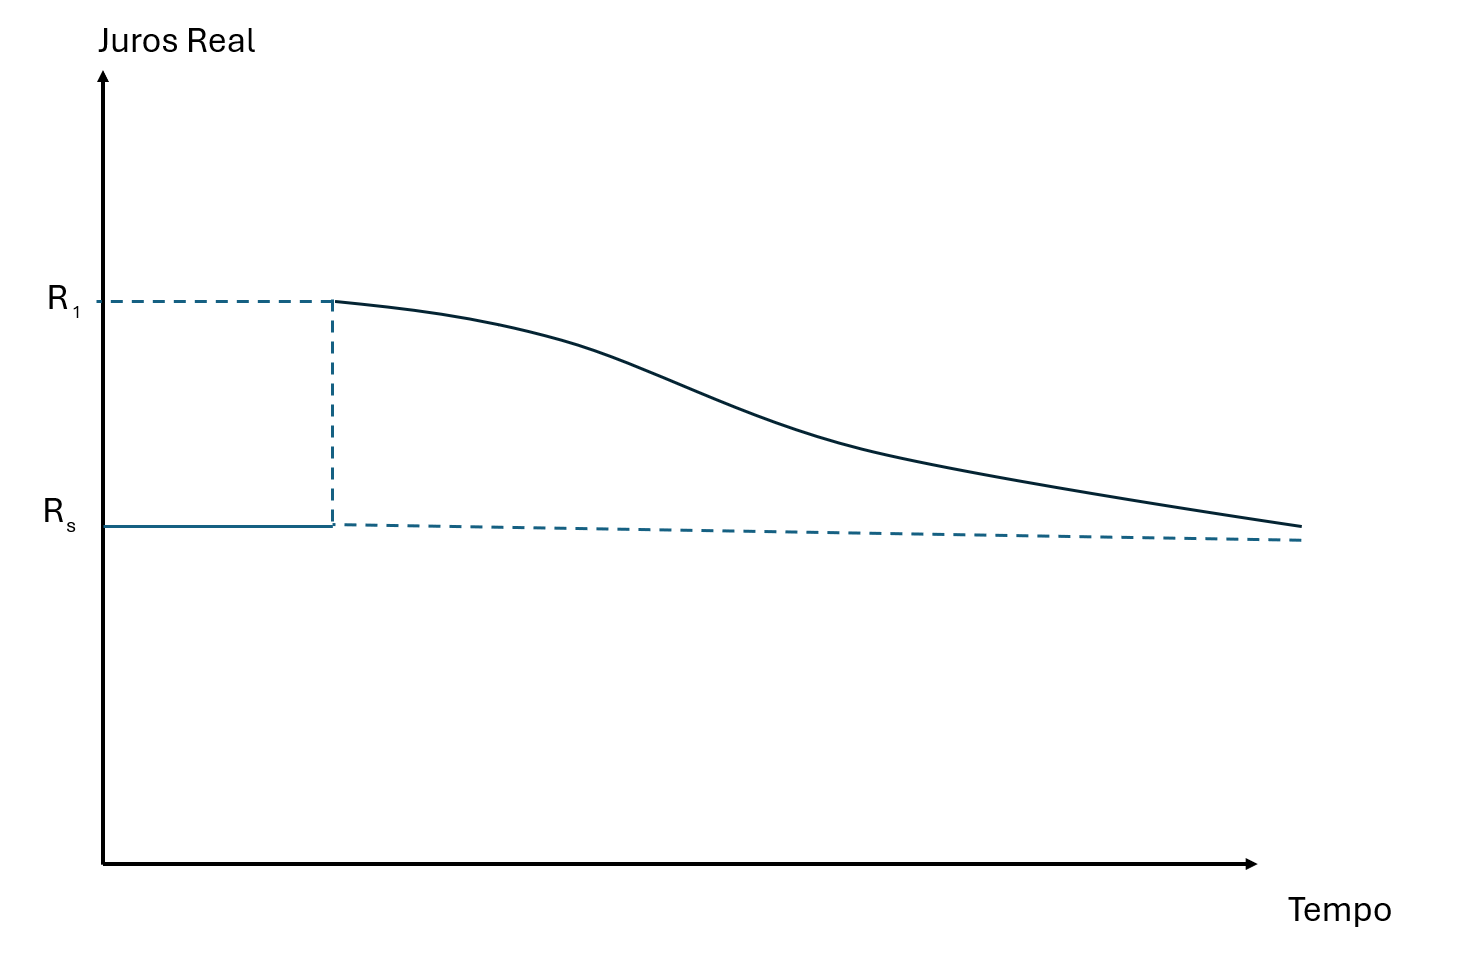
\includegraphics[width=0.7\linewidth]{Imagens/a2i2.png}
        \end{figure}
    \end{enumerate}
    \item  E se tiver um choque positivo de demanda por emprego ($\uparrow E^d$) dado o exemplo de imigrantes?\begin{enumerate}
        \item Um choque positivo de emprego ocasiona, dependendo da qualificação dessa população, um choque de produtividade, incrementando o produto (choque de oferta) ou um choque de desemprego. 
    \end{enumerate}
\end{itemize}

\begin{figure}[H]
    \centering
    \caption{Esquema de Ação do Banco Central frente a desequilíbrios inflacionários}
    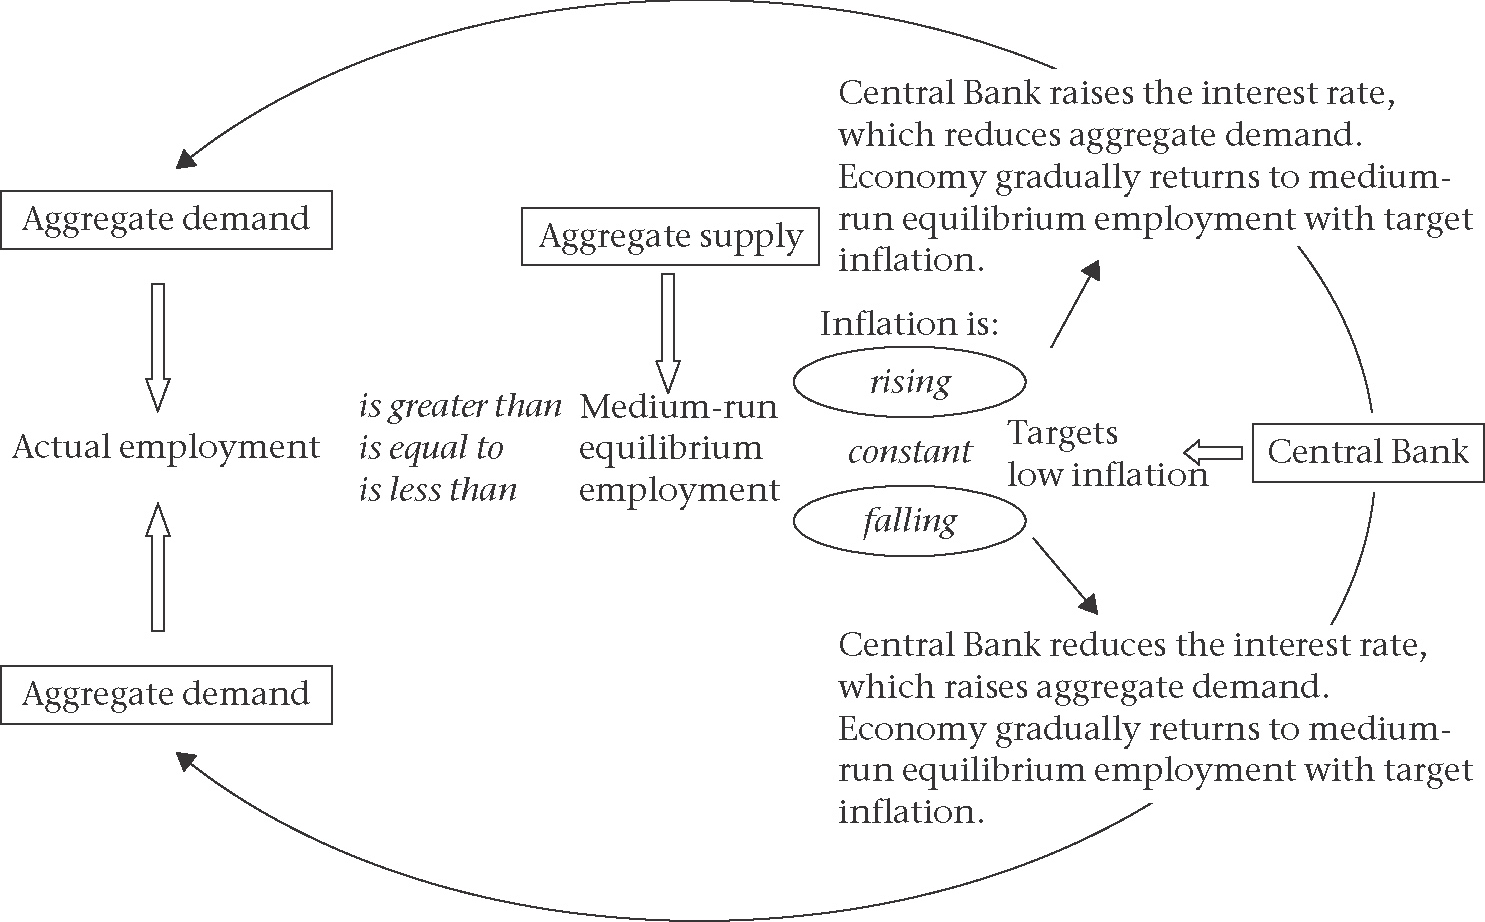
\includegraphics[width=0.7\linewidth]{Imagens/a1i1.png}
\end{figure}

Estabilidade inflacionária$\rightarrow$ hiato do produto é igual a zero. \textbf{Cuidado}, pois o mercado de trabalho pode estar em equilíbrio, mas não se ter estabilidade inflacionária. Isso pois é possível se colocar o mercado de trabalho em equilíbrio a um nível inflacionário acima ou abaixo do nível consistente com as metas inflacionárias. 

\subsection{\textbf{Síntese}}
Antecipando alguns resultados fundamentais:\begin{enumerate}
    \item No curto prazo, os níveis de emprego e produção são determinados pelo nível de demanda agregada da economia
    \item Há uma única taxa de desemprego de equilíbrio no médio prazo consistente com a estabilidade inflacionária \begin{enumerate}
        \item a essa taxa de desemprego a remuneração real dos trabalhadores é aquela que compatibiliza as demandas dos trabalhadores e as demandas das empresas
        \item remuneração real dos trabalhadores = remuneração que as firmas topam pagar
        \item características estruturais e institucionais determinam a taxa de desemprego de equilíbrio
    \end{enumerate}
    \item Em geral há desemprego involuntário: existem trabalhadores dispostos a trabalhar ao nível salarial corrente mas que não estão empregados - em especial sob condições de concorrência imperfeita.
    \item Se o nível de demanda agregada gera uma taxa de desemprego abaixo da taxa de equilíbrio de médio prazo, a inflação tenderá a subir; se a taxa de desemprego exceder a taxa de equilíbrio de médio prazo, a inflação tenderá a cair.
    \item Se os formuladores de políticas perseguem uma meta de inflação, a economia tenderá a retornar ao nível de desemprego de equilíbrio depois de um choque inesperado sobre a demanda agregada; a velocidade de transição para o equilíbrio depende do funcionamento dos mercados e de traços institucionais.
\end{enumerate}

\newpage
\section{\textbf{Demanda, oferta, flutuações}}
\subsection{\textbf{Revisão IS-LM}}
A estrutura do modelo é dada por três equações:\begin{itemize}
    \item Função IS $\Rightarrow$ \textbf{IS}
    \item Curva de Phillips $\Rightarrow$ \textbf{PC}
    \item Regra Monetária $\Rightarrow$ MR \begin{itemize}
        \item A regra monetária é uma função de reação do BC, resultante das preferências assoaciadas ao \textit{trade-off} entre inflação e desemprego
    \end{itemize}
\end{itemize}

\subsection{\textbf{Equilíbrio no Mercado de Bens: Demanda Agregada e IS}}
\textbf{IS}$\rightarrow$descreve o equilíbrio no mercado de bens, sendo determinada pela igualdade entre os níveis de  oferta de  produto e  demanda  por  produto  no  curto  prazo. Assim,  define-se  os elementos que  compõem  essa  curva  por  serem os mesmos  que  compõem a  equação da demanda agregada por bens e serviços: $y^d=c(y,t,riqueza)+I(r,A)+g$\begin{itemize}
    \item \textbf{1º OBS} Impactos marginais em c:\begin{enumerate}
        \item y $\rightarrow$ \textbf{+}
        \item t $\rightarrow$ \textbf{-}
        \item riqueza $\rightarrow$ \textbf{+}
    \end{enumerate} 
    \item \textbf{2º OBS} Impactos marginais em I:\begin{enumerate}
        \item r $\rightarrow$ \textbf{-}
        \item A $\rightarrow$ \textbf{+}
    \end{enumerate} 
\end{itemize}

Função IS, equação:
$$y=y^d=c_0+c_y(1-t_y)y+A-ar+g$$
Note \begin{itemize}
    \item $I = A-ar$, sendo $a$ = sensibilidade à taxa real de juros
    \item Depende de um componente exógeno, refletindo as intenções de gasto tanto do setor público como do setor público como do setor privado
    \item Depende inversamente da taxa real de juros, através dos componentes de gasto sensíveis a elas(consumo e investimento): $-ar$
    \item equilíbrio no mercado de bens, dada pela igualdade entre demanda e produção 
    \item demanda = gasto real  em bens e serviços = $y^D$
    \item equilíbrio requer igualdade entre gasto  de bens e serviços e oferta real $y^D=y$ define a curva IS 
\end{itemize}

\subsection{\textbf{Demanda Total}}
A demanda total é composta pela absorção doméstica da produção local, gasto do setor privado em consumo e investimentos e pelos gastos do governo $\rightarrow y^D=c(y,t,riqueza)+I(r,A)+g$ 

\subsection{\textbf{Consumo}}
A função consumo $c =c (y,t,riqueza) =c_0+c_y(y-t)$ é composta por: \begin{itemize}
    \item $c_0$ é o componente autônomo do consumo que depende de fatores como riqueza
    \item $c_y$ é a proporção da renda corrente que é consumida e satisfaz $0<c_y<1$, além disso ela é a propensão marginal a consumir(da renda) $\frac{\partial}{\partial y}c$ 
    \item onde $(1-t_y)y$ é chamada de renda disponível e $1-c_y=s_y$ é chamada de propensão marginal a poupar
    \item como a tributação satisfaz $t=t_yy$, segue que o consumo $c = c_0+c_y(y-t)=c_0+c_y(y-t_yy)=c_0+c_y(1-t_y)y$
\end{itemize}

\subsection{\textbf{Investimento}}
A função investimento $I=I(r,A)=A-ar$ depende de variáveis(potencialmente exógenas) como produtividade, expectativas, "\textit{animal spirits}", sintetizadas pelo parâmetro A.\begin{itemize}
    \item depende  negativamente do custo de capital, definido pela taxa real de juros, $r$
    \item o parâmetro $a$ mede a sensibilidade da função investimento à taxa real de juros
\end{itemize}

\subsection{\textbf{Demanda Agregada}}
A economia fechada inicialmente: a soma dos componentes domésticos da demanda é uma função linear
$$
y^D=c_0+c_y(y-t)+I(r,A)+g \rightarrow c_0+c_y(1-t_y)y+A-ar+g
$$

\subsection{\textbf{Equilíbrio no Mercado de Bens}}
O equilíbrio no mercado de bens, dado pela igualdade entre demanda e oferta, deifine a curva \textbf{IS}. Demanda $=$ gasto real  em bens e serviços $=y^D$. O equilíbrio requer igualdade entre oferta real e gasto  em bens e gasto  em bens e serviços.
\begin{align*}
    y &= y^D \\
    y &= c_0 + c_y (1 - t_y)y + A - ar + g \\
    y[1 - c_y(1 - t_y)] &= c_0 + A + g - ar \\
    y &= \frac{c_0 + A + g}{1 - c_y(1 - t_y)} - \frac{a}{1 - c_y(1 - t_y)}r \\
    y &= \frac{c_0 + A + g}{s_y + c_y t_y} - \frac{a}{s_y + c_y t_y}r
\end{align*}
Temos que a propensão marginal a poupar $s_y=1-c_y$ e $\frac{1}{s_y+c_yt_y}=\frac{1}{1-c_y(1-t_y)}$ é o multiplicador do gasto autônomo. \begin{itemize}
    \item $\uparrow t_y$, resulta em um menor multiplicador
    \item $1=c_y+s_y$, sendo $s_y$ a proporção marginal a consumir
    \item Assim, $\uparrow s_y$resulta em um menor multiplicador
    \item $(c_o+A+g-ar)$ : para uma dada taxa de juros são os componentes exógenos de demanda
    \item Observe que o multiplicador é afetado pelos "vazamentos" de demanda associados à poupança à tributação. O multiplicador captura o efeito de retoralimentação entre renda disponível e demanda. Se te mais renda indo para o governo(receitas fiscais), ou seja, \(\uparrow t_y\), sobre menos renda para o consumo. 
    \item Podemos representar o multiplicador da seguinte forma também: 
    \[
    \frac{1}{1-c_y(1-t_y)}=\frac{1}{1-(1-s_y)(1-t_y)}=\frac{1}{1-1+t_y+s_y-s_yt_y}=\frac{1}{t_y+s_y(1-t_y)}
    \]
\end{itemize}

\textbf{IS} estabelece o nível de investimento associado a uma dada taxa de juros e consequentemente o produto de equilíbrio. Somando-se ao investimento o gasto autônomo em consumo e a demanda do governo e multiplicando-se o resultado pelo multiplicador $\frac{1}{s_y+c_yt_y}$ obtém-se o produto de equilíbrio. poupança e tributação representam “vazamentos" no processo de transformação da renda em gastos. Inclinação negativa resulta de um maior nível de investimento e consequentemente do produto estar associado a uma taxa de juros mais baixa: equação da \textbf{IS} no plano [$r,y$]

\begin{align*}
    r &= \frac{c_0 + A + g_0}{a} - \frac{(1 - c_y(1 - t_y))}{a}y \\
    \frac{dr}{dy}\bigg|_{IS} &= \frac{-(1 - c_y(1 - t_y))}{a} < 0
\end{align*}

\begin{figure}[H]
    \centering
    \caption{Função e Deslocamento da Curva IS}
    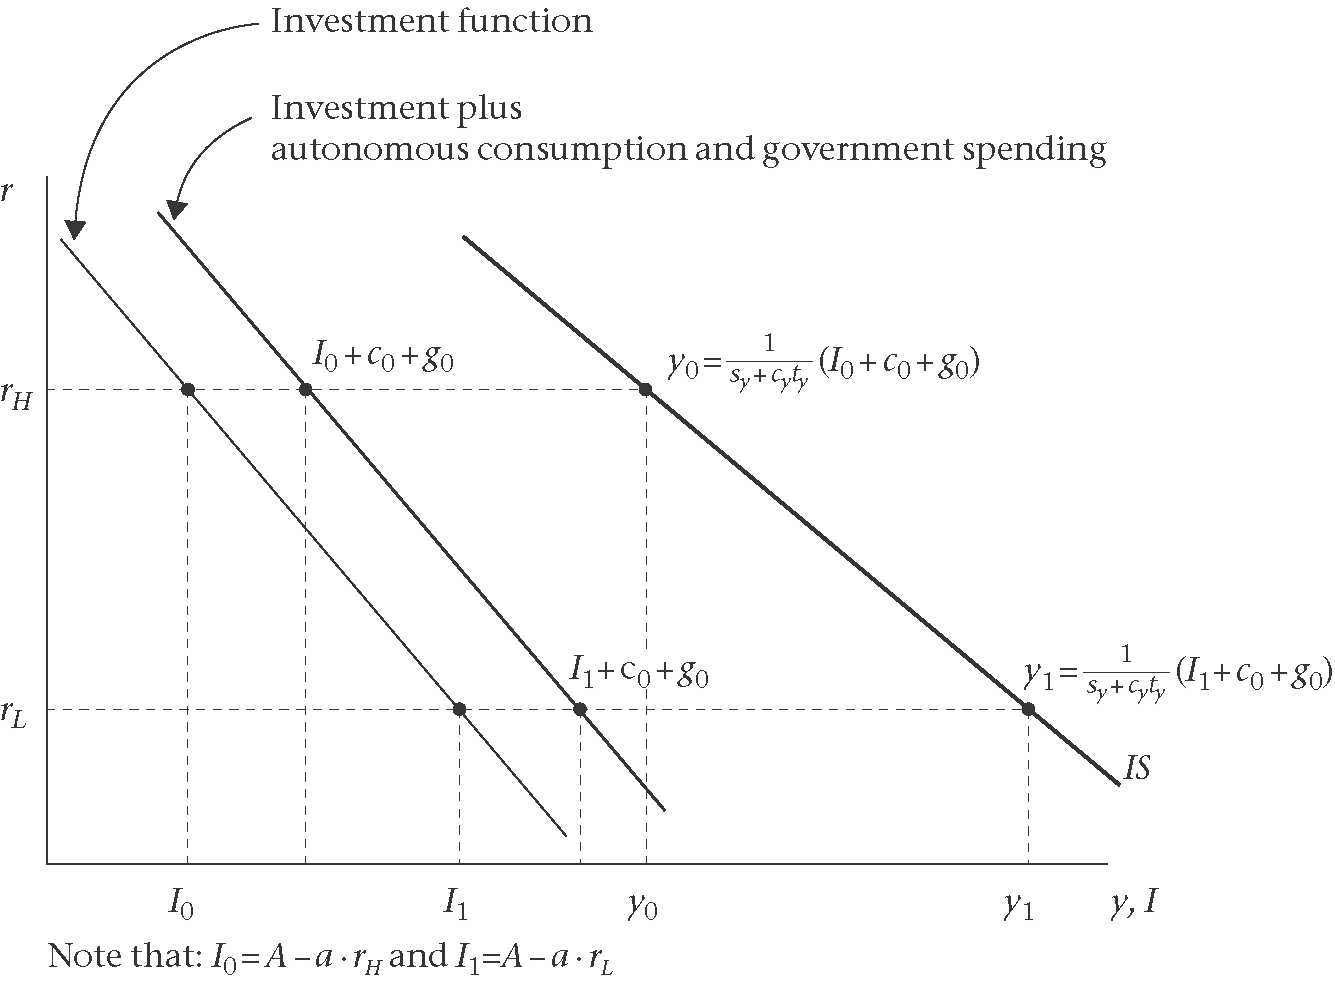
\includegraphics[width=0.75\linewidth]{Imagens/a2i1.png}
\end{figure}



O multiplicador afeta a inclinação\begin{itemize}
    \item maior $c_y$ leva a um maior multiplicador tornando a curva menos inclinada(mais horizontal)
    $$
    \frac{d^2r}{dydc_y}\bigg|_{IS}=\frac{1-t_y}{a}>0
    $$
\end{itemize}

Elasticidade do investimento com relação a $r$ afeta a inclinação\begin{itemize}
        \item quanto maior a sensibilidade de $I$ a $r$, menos inclinada a curva(mais horizontal)
        $$
        \frac{d^2r}{dyda}\bigg|_{IS}=\frac{(1-c_y(1-t_y))}{a^2}>0
        $$
    \end{itemize} 

Um incremento na propensão marginal a consumir(\(\uparrow c_y\)) torna a curva da função IS mais horizontal. Racional: O aumento na propensão marginal a consumir ocasiona um aumento em renda disponível  \((y − t)\),  ocasionando,  via  mudança  do  multiplicador  (maior),  um  maior  efeito marginal na demanda agregada quando se tem uma variação na taxa real de juros.
\begin{figure}[H]
    \centering
    \caption{Deslocamento da IS dado aumento do consumo marginal}
    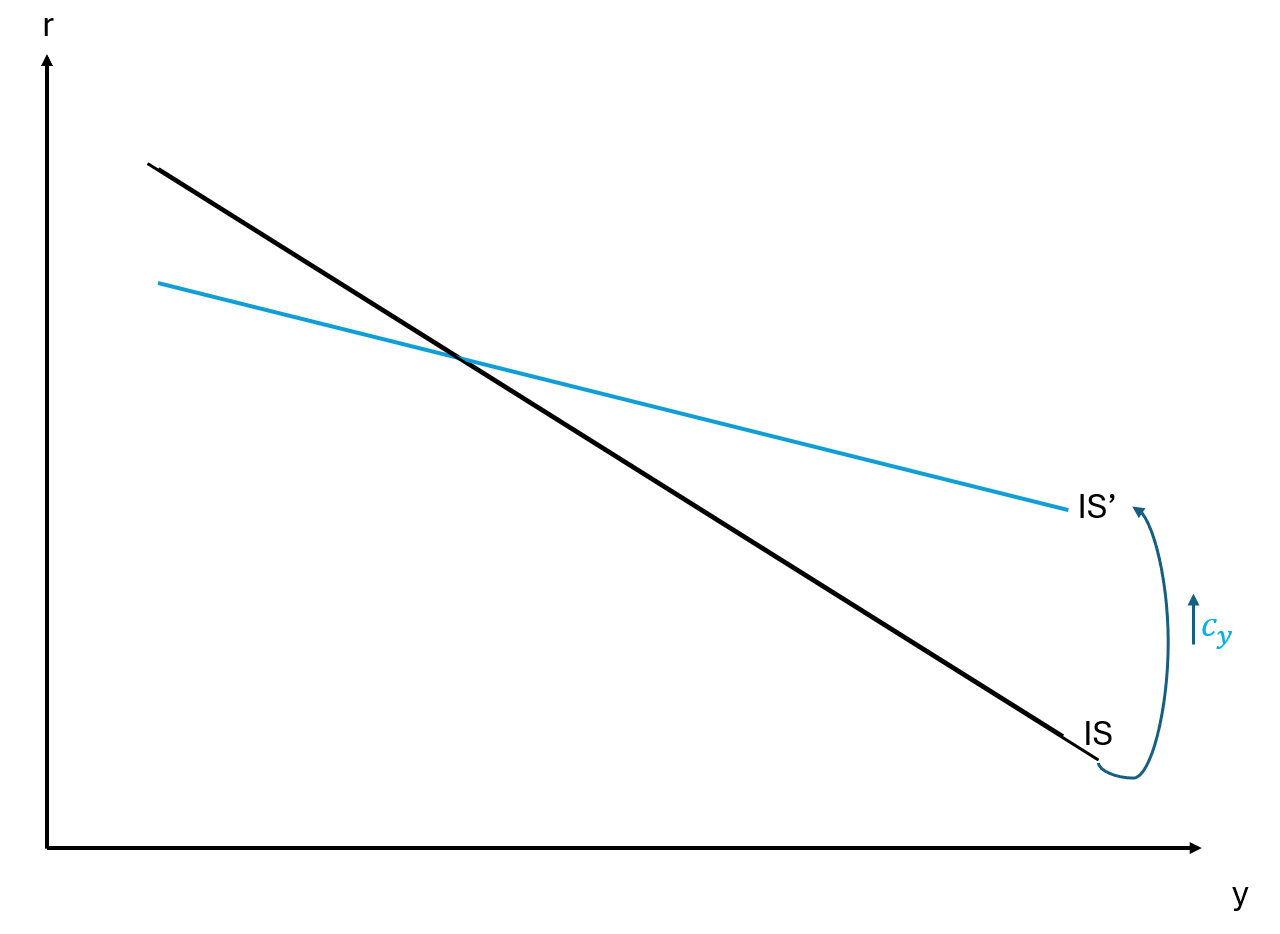
\includegraphics[width=0.7\linewidth]{Imagens/a2i4.png}
\end{figure}

Pelo mesmo canal da renda disponível, alterações positivas na propensão marginal a tributar faz com que a curva da função IS se torne mais verticalmente inclinada . 

\begin{figure}[H]
    \centering
    \caption{Deslocamento da IS dado aumento do tributação marginal}
    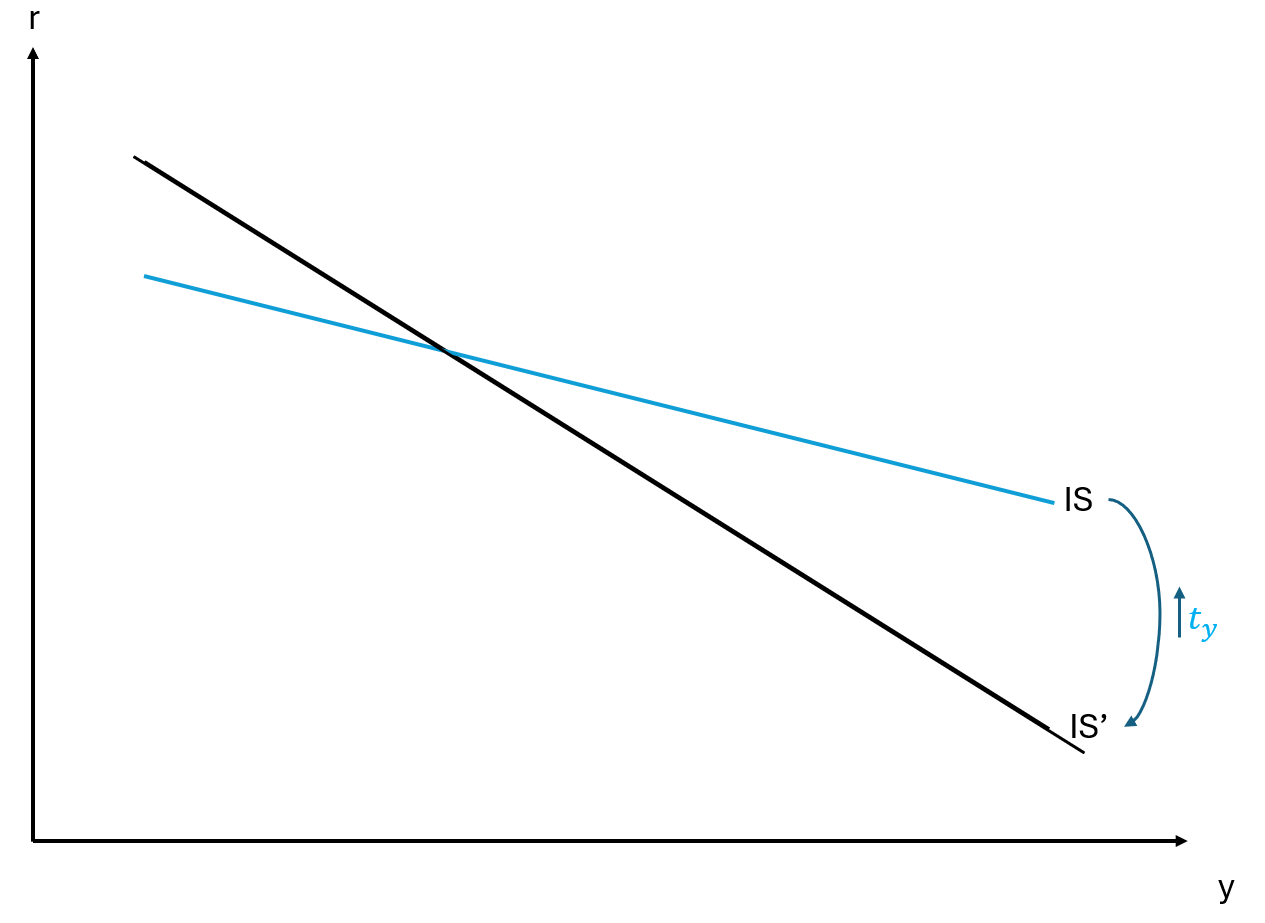
\includegraphics[width=0.75\linewidth]{Imagens/a2i5.png}
\end{figure}

Mudanças no gasto autônomo privado ou público, $c_0$ e $g_0$, deslocam \textbf{IS}. Menor $t_y$ eleva o multiplicador e torna a \textbf{IS} mais horizontal $\Rightarrow$ deslocamento da curva para a direita. Maior $g_0$ desloca a curva para a direita pela magnitude do incremento no gasto autônomo vezes o multiplicador: $\Delta g \times \frac{1}{s_y+c_yt_y}$

\subsection{\textbf{Ajuste das Quantidades}}
Duas dimensões do ajuste de quantidade no curto prazo:\begin{itemize}
    \item o processo multiplicador
    \item variações nos estoques
\end{itemize}

Equilíbrio de curto prazo é atingido através das variações das quantidades mediadas pelo processo multiplicar

No primeiro \textit{round} $\Delta c=c_y\Delta y$; mas esse choque reduz adicionalmente a demanda (e o produto) deprimindo o consumo ainda mais. No segundo \textit{round} $\Delta c=c_y(c_y\Delta y)=c_y^2\Delta y$. No terceiro \textit{round}$\Delta c=c_y(c_y(c_y\Delta y))=c_y^3\Delta y$. Ainda sim sucessivamente. O impacto cumulativo 
\begin{align*}
    \Delta y &= \Delta I + c_y \Delta I + c_y^2 \Delta I + c_y^3 \Delta I + \dots \\
             &= (1 + c_y + c_y^2 + c_y^3 + \dots)\Delta I \\
             &= \frac{1}{1 - c_y} \Delta I
\end{align*}

\textbf{1ª interação (queda inicial em investimento):}

\[
y^d = c(y) + I \quad \leftarrow \text{choque: } \Delta I < 0
\]
\[
\downarrow y = \downarrow y^d = c_y \cdot y + \downarrow I
\]

\textbf{2ª interação:}
\[
\Delta y_1 = c_y \cdot \Delta y_0 + \Delta I
\]

A variação inicial da renda afeta a renda novamente.

\textbf{3ª interação:}
\[
\Delta y^c = c_y \cdot \Delta y + c_y^2 \cdot \Delta y + \Delta I
\]

"c" de impacto cumulativo.

\textbf{nª interação:}

\begin{enumerate}
    \item[(a)] 
    \[
    \Delta y^c = c_y \Delta y + c_y^2 \Delta y + \dots + c_y^{n-1} \Delta y + \Delta I
    \]
    \item[(b)] Levando em consideração que \( \Delta I = \Delta y \) nesse contexto, tem-se que:
    \[
    c_y \Delta y^c = \Delta I (c_y + c_y^2 + c_y^3 + \dots + c_y^n)
    \]
\end{enumerate}

Assim, subtraindo "(a)" de "(b)", obtém-se:
\[
\Delta y^c - c_y \Delta y^c = \Delta I [1 - c_y^n]
\]
\[
\Delta y^c [1 - c_y] = \Delta I [1 - c_y^n]
\]
\[
\Delta y^c = \Delta I \cdot \frac{1 - c_y^n}{1 - c_y}
\]
\[
\lim_{n \to \infty} \Delta y^c = \frac{\Delta I}{1 - c_y} * \lim_{n \to \infty} \left[1 - c_y^n\right]
\]

Note que:
\[
\lim_{n \to \infty} c_y^n = 0
\]

Assim, fica:
\[
\Delta y^c = \frac{\Delta I}{1 - c_y}
\]

Conclui-se, portanto, que o produto/renda varia como um múltiplo do choque exógeno.
\begin{figure}[H]
    \centering
    \caption{Deslocamento da IS dado aumento do Investimento e Efeito do multiplicador}
    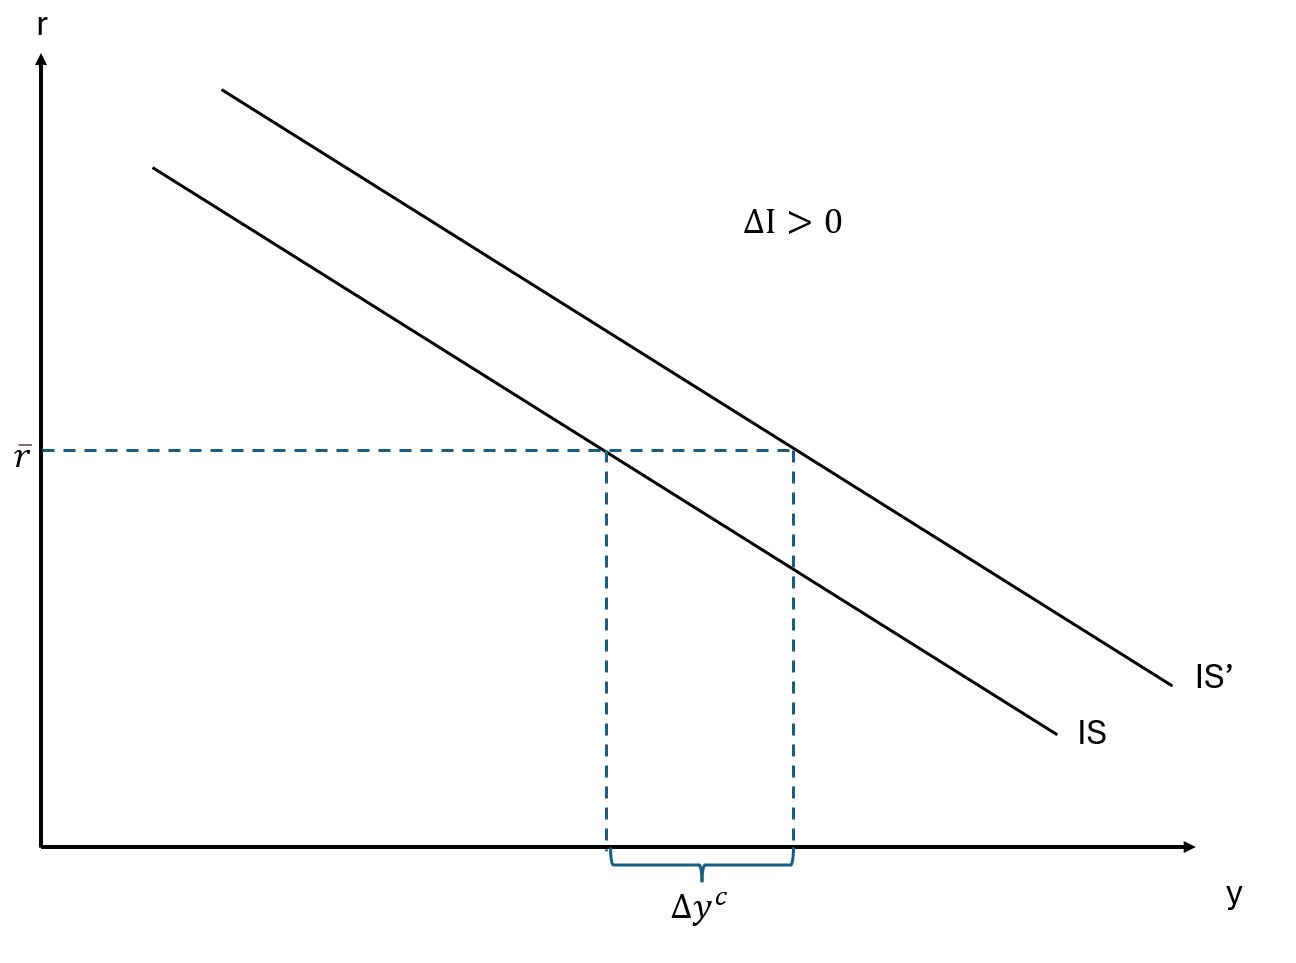
\includegraphics[width=0.7\linewidth]{Imagens/a2i6.png}
\end{figure}

A ideia por trás dessas interações é a de que o choque em uma variável exógena (investimento) iniciou um processo de diminuição na demanda por bens e serviços e renda, que gera uma diminuição no consumo, o que diminui o nível de atividade e, consequentemente diminui novamente a demanda por bens e serviços e renda. Assim, cria-se um ciclo infinito e cumulativo de diminuição da demanda por bens e serviços e da renda. 

A contração do produto é um múltiplo do choque original. O produto se contraí até gerar um nível de poupança igual ao menor nível de investimento. Ajuste via estoques: \begin{itemize}
    \item $y>y^d$ 
    \item $y<y^D$
\end{itemize}

Abaixo e à esquerda de \textbf{IS} há excessso de demanda no mercado de bens pois, à taxa de juros $r_1$ o gasto é $y_1>y_x \Rightarrow$ estoques caem e produto cresce até atingir \textbf{IS}. Acima e à direita de \textbf{IS} há excesso de oferta no mercado de bens pois, à taxa de juros $r_1$ o gasto é $y_1<y_z \Rightarrow$ estoques aumentam e produto diminui até atingir \textbf{IS}

\begin{figure}[H]
    \centering    
    \caption{Desequilíbrios na IS}
    
\includegraphics[width=0.75\linewidth]{Imagens/a2i3.png}
\end{figure}

\subsection{\textbf{Mercado Monetário e LM}}

\textbf{LM}: escreve o equilíbrio no mercado monetário a partir de uma igualdade entre a demanda por liquidez e oferta de moeda, enquanto preconiza um controle de um agregado monetário (seja via \(M \ ou \ \frac{\Delta M}{M}\))

Demanda por moeda é uma demanda por liquidez $\frac{M^D}{P}=L(y,i)$ sendo $i$ a taxa nominal de juros. $L$ expressa em termos reais, uma quantidade de poder de compra sob a forma líquida: \begin{itemize}
    \item $L$ é expressa em termos reais, uma quantidade poder de poder de compra sob a forma líquida: a demanda nominal por moeda é proporcional ao preços $M^D=P \times L(y,i)$(sendo essa a representação da função LM)
    \item$L$ é crescente na renda, $\frac{\partial L}{\partial y}>0$, refletindo a demanda por moeda para transações. $L$ é decrescente com uma maior taxa de juros, $\frac{\partial L}{\partial i}<0$, refletindo o custo de oportunidade de reter moeda, o rendimento a que se renuncia por manter um ativo cujo retorno nominal é nulo. 
\end{itemize}

Sendo \(M^d\)   a demanda nominal por moeda. E \(L(y, i)\) é a demanda real por liquidez. Assim, a demanda  real por liquidez se traduz por ser a demanda  real por poder de compra dos consumidores, investidores e empresas sobre a forma líquida. 

É observável que variações em renda/produção causam efeitos marginais positivos na demanda real por liquidez; enquanto variações na taxa nominal de juros causam efeitos marginais negativos na demanda real por liquidez. 

Alocação da riqueza financeira: para facilitar, são dados dois caminhos, a Moeda e os Títulos. A Moeda não rende juros, mas é líquida, enquanto os Títulos rendem juros, mas não podem ser trocados. Assim, quanto maior a taxa de juros, maior o custo de oportunidade de se reter a moeda (taxa de juros) e, por consequência, a demanda real por liquidez é deprimida.  

É possível expressar a demanda por moeda como uma função linear da renda e da taxa de juros:
$$
\frac{M^D}{P}=\underbrace{l-l_ii}_\text{Demanda por Ativo} + \underbrace{\frac{1}{v_T}y}_\text{Demanda para Transações}
$$

\begin{itemize}
    \item $l$: parâmetro de demanda por liquidez autônoma
    \item $l_i$: sensibilidade da demanda real por liquidez à taxa nominal de juros
    \item $V_T$: velocidade de circulação da moeda
    \item $l - l_ii$: demanda por ativos (bens que rendem juros) $\quad \rightarrow \quad$ parte sensível à taxa nominal de juros.
    \item $\frac{1}{V_T} \cdot y$: demanda por liquidez para transações (ex.: pagar o Insper, consumo) $\quad \rightarrow \quad$ parte sensível à renda.
    \item $M^d$ Demanda Nominal por Moeda
    \item $\frac{M^D}{P}$ Demanda Real por Liquidez
\end{itemize}


\textbf{Por  que  estudar  a LM,  se  futuramente  utilizaremos  a  regra  monetária  para  analisar  os mercados? }

\textbf{Resposta}: Porque existem duas formas diferentes de se abordar a implementação de uma política monetária: uma que observa o controle dos estoques monetários e outra que observa o controle sobre a taxa de juros. A função LM captura de forma mais sintética e clara o controle da quantidade de moeda em circulação e as relações entre demanda por liquidez e oferta de moeda. \begin{itemize}
    \item A LM ainda descreve o eq. no mercado monetário, mesmo quando se tenha um contexto em que o Banco Central opera uma regra de juros (fixar). 
    \item Nos cenários em que se tem uma armadilha de liquidez, a LM se mostra ser mais bem equipada como ferramenta de análise do que a MR, por exemplo. 
    \item A LM ainda é usada na análise das economias abertas, pois captura melhor como ferramenta  de  estudo  as  expectativas  sobre  a  taxa  de  câmbio  que  impactam  a determinação da taxa de câmbio corrente. Até poderia, via PDJ, analisar economias abertas  usando  regras  de  juros  (MR),  mas  vale  apontar  que  estas  não  levam  em consideração as expectativas sobre a taxa de câmbio. 
\end{itemize}

Sendo $M^d$ a demanda nominal por moeda. E $L(y,i)$ é a demanda real por liquidez. Assim, a demanda  real  por  liquidez  se  traduz  por  ser  a  demanda  real  por  poder  de  compra  dos consumidores, investidores e empresas sobre a forma líquida. 

É observável que variações em renda/produção causam efeitos marginais positivos na demanda real por liquidez; enquanto variações na taxa nominal de juros causam efeitos marginais negativos na demanda real por liquidez. 
Alocação da riqueza financeira: para facilitar, são dados dois caminhos, a Moeda e os Títulos. A Moeda não rende juros, mas é líquida, enquanto os Títulos rendem juros, mas não podem ser trocados. Assim, quanto maior a taxa de juros, maior o custo de oportunidade de se reter a moeda (taxa de juros) e, por consequência, a demanda real por liquidez é deprimida.  

\textbf{MR} $\rightarrow$ Apresenta um  direcionamento um pouco diferente  daquele  apresentado pela  LM, evidenciando as relações que determinam o controle que Banco Central faz sobre a taxa de juros nominal (i). A MR traz uma perspectiva que inclui a taxa de juros como um termo endógeno.

Como é calculada a velocidade de circulação da moeda ($v_T$)? Suponha $(l - l_i \cdot i) = 0$, ou seja, a demanda real por liquidez sendo 100\% igual à demanda por transações:
\[
\frac{M^d}{P} = \frac{y}{v_T} \quad \rightarrow \quad M^d \cdot v_T = P \cdot y\rightarrow v_T=\frac{P \cdot y}{M^D} (\text{"giro/tempo''})
\]

\begin{itemize}
    \item \textbf{APARECE A TEORIA QUANTITATIVA DA MOEDA}
    \item Essa equação torna evidente o Produto Nominal da Economia, que é $P \cdot y$: o preço da cesta multiplicado pelo tamanho da cesta.
\end{itemize}

Quanto maior a taxa de juros, maior o custo de oportunidade de reter a moeda. Assim, títulos passam a se tornar cada vez mais atrativos.

Quando a taxa de juros é 10\%. Um título com valor de face de \$100 e cupom de 10\%. A cada ano eu recebo \$10 do cupom. Se a taxa de juros subir para 20\%, para que o título renda 20\% do cupom, o seu valor de negociação terá de ser mais baixo. Perceba que independente das mudanças da taxa de juros, o valor de face sempre será o mesmo, o que pode mudar é o valor de negociação. Assim, o preço de venda negociado do título de 10\% terá de ser mais baixo, gerando perdas de capital. O termo $(l - l_i \cdot i)$ então representa a parte da demanda real por liquidez que se protege dessas perdas de capital provenientes de um potencial aumento na taxa de juros (Por que irei comprar um título hoje se acredito que a taxa de juros irá subir amanhã?).

A função LM, portanto, é aquela que expressa o equilíbrio no mercado monetário:
\[
\frac{M^s}{P} = \frac{M^d}{P} = L(y, i)
\]

\begin{itemize}
    \item Sendo $\frac{M^s}{P}$ oferta real de moeda (controlado pelo BACEN)
\end{itemize}

LM descreve as combinações de taxa de juros e produto($i,y$) consistentes com o equilíbrio no mercado monetário ($M^s(\text{instrumento de política monetária e geralmente definido pelo BC}) = M^d$).

\textbf{A diferença entre a demanda por moeda para transações e a demanda por moeda como ativo é a seguinte:}

A demanda por moeda para transações é a demanda para compras e vendas diárias. Inclui transações de consumidores para bens necessários como arroz, leite, óleo, vegetais, remédios, etc., e transações diárias de empresas e do governo. A demanda por moeda para essas transações é a demanda por transações. Essa demanda é indiferente à taxa de juros prevalecente no mercado ou a quaisquer mudanças nas taxas de juros. Contudo, essa demanda muda com uma variação na renda ou no PIB.

A demanda por moeda como ativo é a demanda para adquirir ativos como títulos, ações, ações preferenciais, debêntures, ouro e outros. O dinheiro necessário para adquirir esses ativos é a demanda por moeda como ativo. É uma forma de manter riqueza. A demanda por moeda como ativo é inversamente afetada pelas mudanças na taxa de juros.

A demanda total por moeda é igual à soma da demanda por transações e da demanda por moeda como ativo. Qualquer mudança na demanda por transações ou na demanda por moeda como ativo altera a demanda total por moeda. A demanda por transações é representada por uma linha vertical, indicando indiferença a mudanças na taxa de juros. Em contraste, a demanda por moeda como ativo é representada por uma curva descendente, indicando sua correlação negativa com as taxas de juros.

Como resultado, a demanda total apresenta inclinação descendente. Quando a taxa de juros muda, a demanda total também muda devido à variação na demanda por moeda como ativo. Da mesma forma, quando o PIB e outros determinantes mudam, a demanda total por moeda muda devido à variação na demanda por transações.

A curva LM é positivamente inclinada porque para maiores níveis de renda, para que o equilíbrio no mercado monetário seja encontrado, é necessário que o custo de oportunidade de se reter moeda (taxa de juros) seja maior.

\begin{figure}[H]
    \centering    
    \caption{Desequilíbrios na LM}
    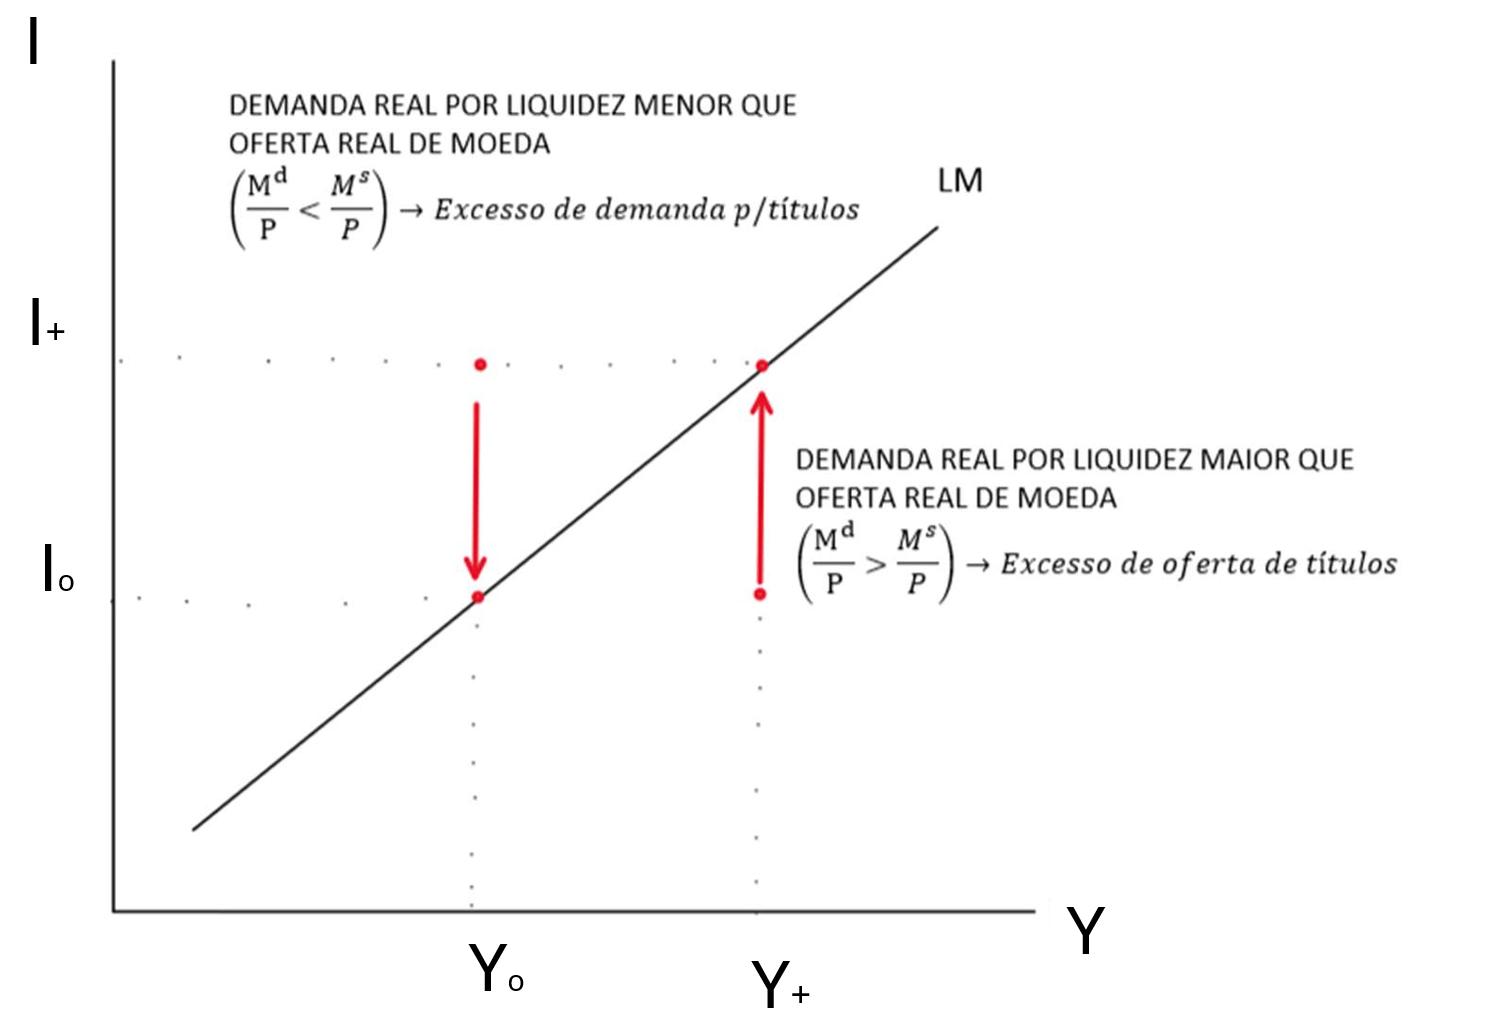
\includegraphics[width=0.75\linewidth]{Imagens/a3i1.png}
\end{figure}

\subsection{\textbf{Equilíbrio}}

Inicialmente assume-se que o Banco Central controla a oferta monetária.

Mais à frente veremos o funcionamento de uma regra monetária baseada na manipulação da taxa de juros.

A curva \textbf{LM} representa as combinações de taxa de juros e produto (ou renda) que equilibram o mercado monetário com igualdade entre demanda e oferta de moeda:
\[
\frac{M^S}{P} = \frac{M^D}{P} = L(y, i)
\]

Equação da \textbf{LM} no plano $[i, y]$:
\[
i = \frac{1}{l_i} \left[ l - \frac{M^S}{P} + \frac{1}{v_T}y \right]
\]

\[
\frac{\partial i}{\partial y}\bigg|_{LM} = \frac{1}{l_i v_T} > 0
\]

\[
i = \frac{1}{l_i} \left[ l - \frac{\uparrow M^S}{P} + \frac{1}{v_T}y \right]
\]
\begin{figure}[H]
    \centering
    \caption{Deslocamento da LM dado variações nas variáveis}
    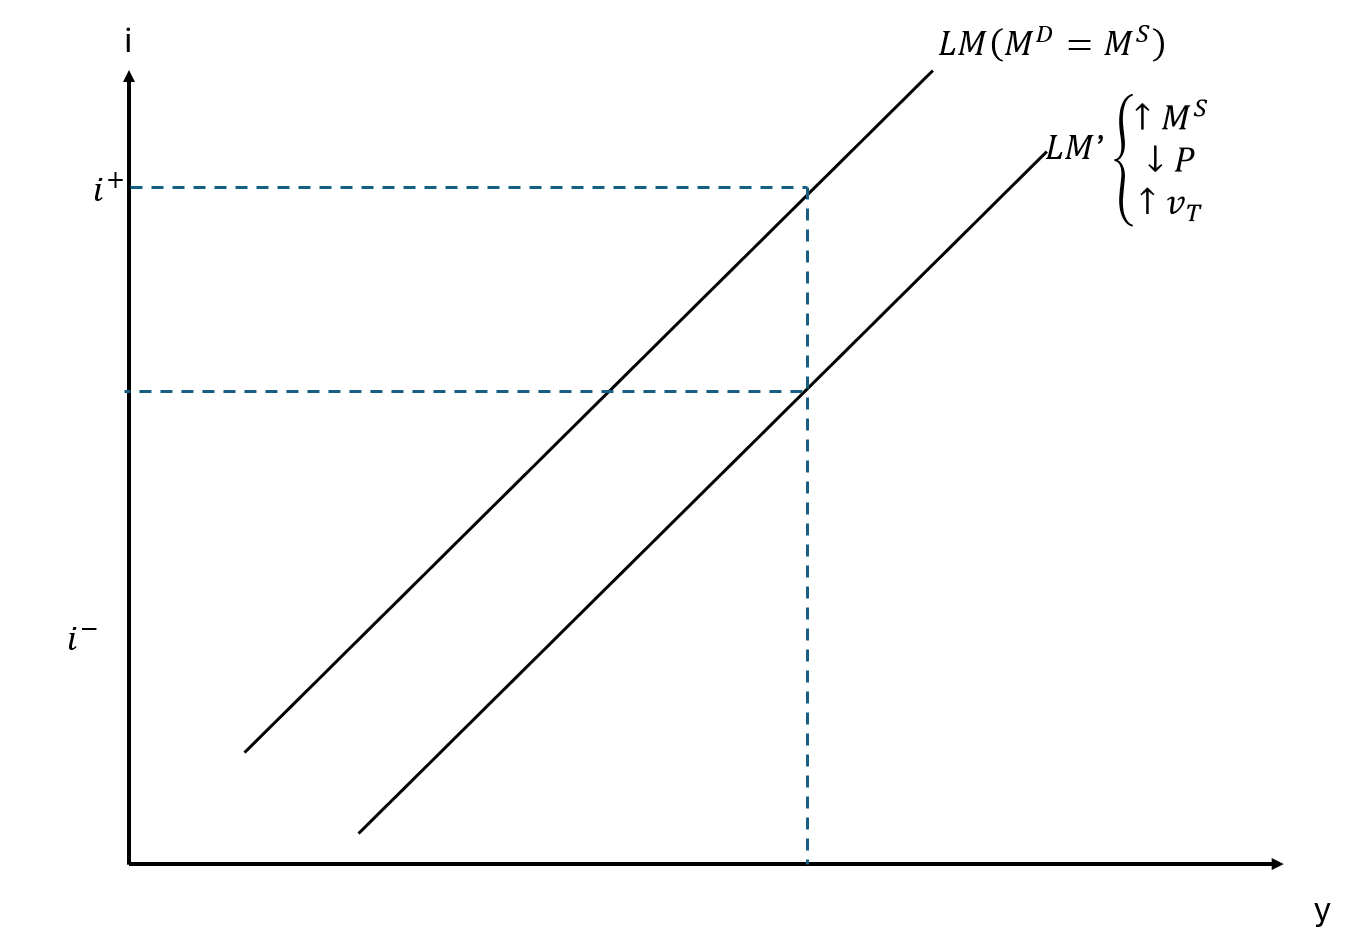
\includegraphics[width=0.75\linewidth]{Imagens/a3i4.png}
\end{figure}

A curva \textbf{LM} tem inclinação positiva: quando $y$ é baixo a demanda por moeda para transações também é baixa; mas como a oferta nominal é fixa, a demanda por moeda como ativo (ou especulativa) deve ser alta, o que requer uma baixa taxa de juros para produzir a igualdade entre oferta e demanda a velocidade de circulação $v_T$ é o número de unidades de renda que uma unidade de moeda (mantida para fins de transação) consegue adquirir.

\begin{figure}[H]
    \centering
    \caption{Deslocamentos e Desequilíbrios da LM}
    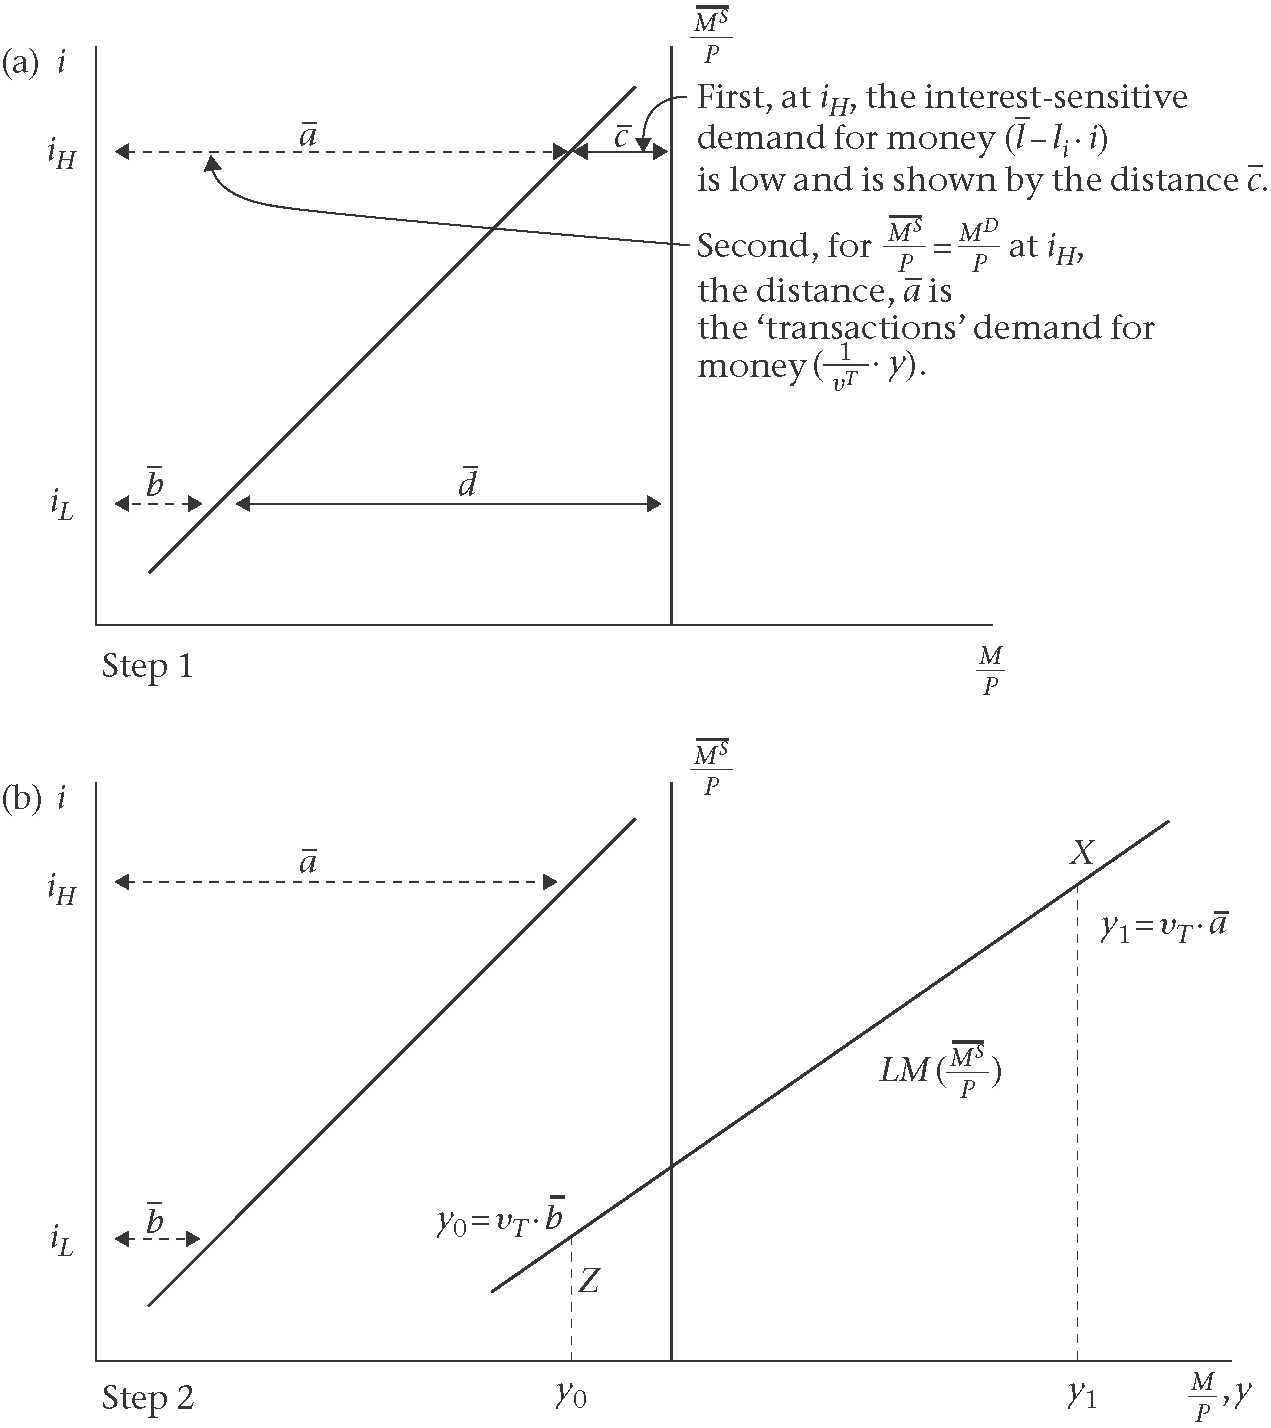
\includegraphics[width=0.75\linewidth]{Imagens/a3i2.png}
\end{figure}

\begin{itemize}
    \item Um aumento na velocidade de circulação $v_T$, refletindo inovações financeiras, por exemplo, leva a uma rotação da \textbf{LM}, tornando-a mais horizontal.
    
    \item Um aumento na sensibilidade da demanda por moeda (como ativo) à taxa de juros $l_i$ torna a curva \textbf{LM} mais horizontal.
    
    \item Um aumento na oferta nominal de moeda desloca a curva \textbf{LM} para a direita, pois requer uma maior demanda por moeda para absorver a oferta excedente: a queda na taxa de juros conjugada ao maior nível de renda eleva a demanda ao nível da oferta um aumento no nível de preços desloca a curva \textbf{LM} para a esquerda, pois, dada a taxa de juros, o menor montante de liquidez real disponível sustenta um menor volume de transações reais.
\end{itemize}

Ajuste de carteira e o equilíbrio no mercado monetário: o que acontece quando oferta e demanda divergem?

Acima e à esquerda de \textbf{LM} há excesso de oferta de moeda no mercado monetário ao nível de renda $y_0$ a taxa de juros $i > i_1$:\begin{itemize}
    \item excesso de oferta de moeda é canalizado para o mercado de títulos: demanda por títulos cresce, aumento seu preço e reduzindo seu rendimento, provocando uma queda na taxa de juros até atingir \textbf{LM}.
\end{itemize}

Abaixo e à direita de \textbf{LM} há excesso de demanda por moeda no mercado monetário ao nível de renda $y_0$ a taxa de juros $i < i_1$:\begin{itemize}
    \item excesso de demanda por moeda é canalizado para o mercado de títulos: oferta de títulos cresce, diminuindo seu preço e aumentando seu rendimento, provocando uma elevação na taxa de juros até atingir \textbf{LM}.
\end{itemize}

\begin{figure}[H]
    \centering  
    \caption{Desequilíbrios da LM}
    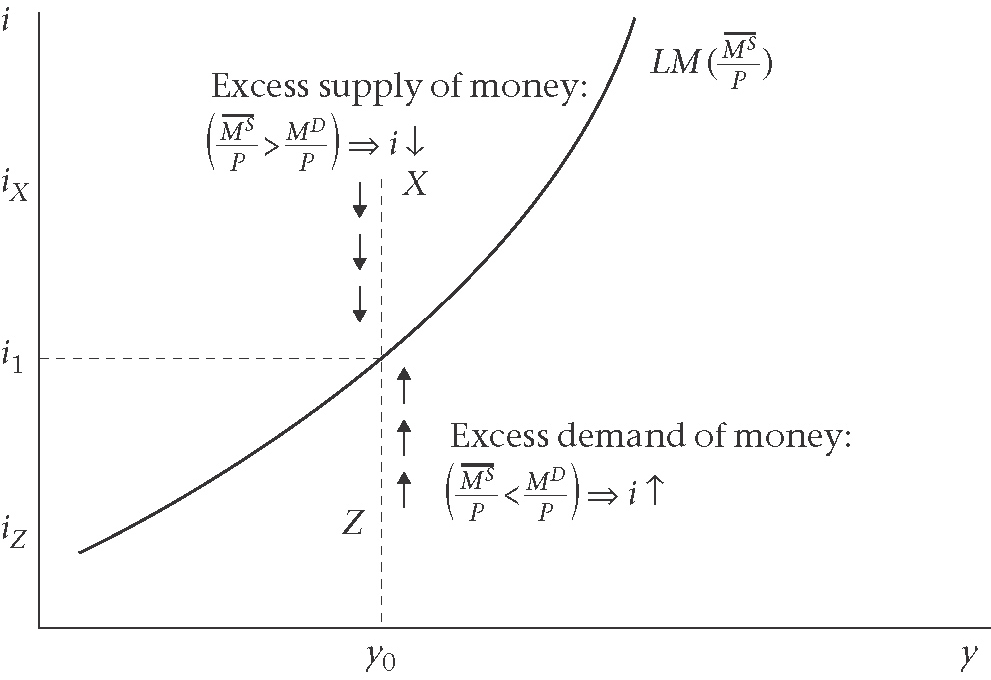
\includegraphics[width=0.7\linewidth]{Imagens/a3i3.png}
\end{figure}

\subsection{\textbf{Integrando os mercados: IS + LM}}
Para se observar as duas curvas que expressam os equilíbrios de produto e taxa de juros para os mercados de bens/serviços (IS) e monetário (LM), molda-se a equação da curva LM para que esta contorne o fator inflacionário e passe a se medir em juros reais, para ficar igual às medidas da IS. Note que originalmente a curva LM se mede em juros nominais. 

\begin{figure}[H]
    \centering
    \caption{IS+LM e pontos de desequilíbrios}
    
\includegraphics[width=0.7\linewidth]{Imagens/a4i1.png}
\end{figure}

Ao combinar os mercados monetários e de bens é possível determinar os valores de equilíbrio no curto da taxa de juros e do produto, para um dado nível de preços. Para isso é necessário uma ponto que conecte a taxa de juros nominal da curva \textbf{LM} à taxa de juros real da curva \textbf{IS}. 

A taxa real de juros $r$ é definida em termo de bens. A taxa nominal de juros $i$ é dinida em termos monetários. A equação de Fisher decompõe a taxa real de juros, $1+r_t=\frac{1+i_t}{1+\pi_t^e}$, com a expectativa de inflação definida por $\pi_t^e=\frac{P_{t+1}^e-P_t}{P_t}$.\begin{itemize}
    \item (1 + $i$) = Fator bruto de juros nominais 
    \item (1 + $r$) = Fator bruto de juros reais 
    \item (1 + $\pi^e$) = Fator bruto de correção inflacionária 
    \item $r=\frac{1+i-\pi^e-1}{1+\pi^e}$\begin{itemize}
        \item $r^e \approx i_t-\pi_t^e$, se $i$ e $\pi^e$ forem pequenos
        \item $r^e$ pode ser obtida; $i$ é observável; $\pi^e$ pode ser estimada/projetada
    \end{itemize}
\end{itemize}

Se os valores da taxa real de juros, da expectativa de inflação e consequentemente da taxa nominal de juros são baixos, vale a aproximação $r_t\approx i_t-\pi_t^e$.

A única variável que pode ser de fato observada é a taxa nominal de juros. A taxa real realizada(ou \textit{ex post}) pode ser calculada a partir da inflação medida. A taxa real esperada (ou \textit{ex ante}) pode ser estimada a partir de um modelo de projeção de inflação.

Vamos supor inicialmente que $\pi^e=\pi=0$, $r=i$, interseção define o equilíbrio macro de longo prazo. \begin{itemize}
    \item Produto e juros de equilíbrio no mercado de bens e monetário. Desequilíbrios no mercado de ativos são eliminados rapidamente$\rightarrow$ ajuste é veloz e se materializa através da mudança no preço dos títulos nos mercados financeiros.
    \item Desequilíbrios no mercado de bens são eliminados mais lentamente$\rightarrow$ ajuste é mais lento pois requer alteração da produção e do emprego.
\end{itemize}

\begin{figure}[H]
    \centering
    \caption{Resolvendo os desequilíbrios na IS-LM}
    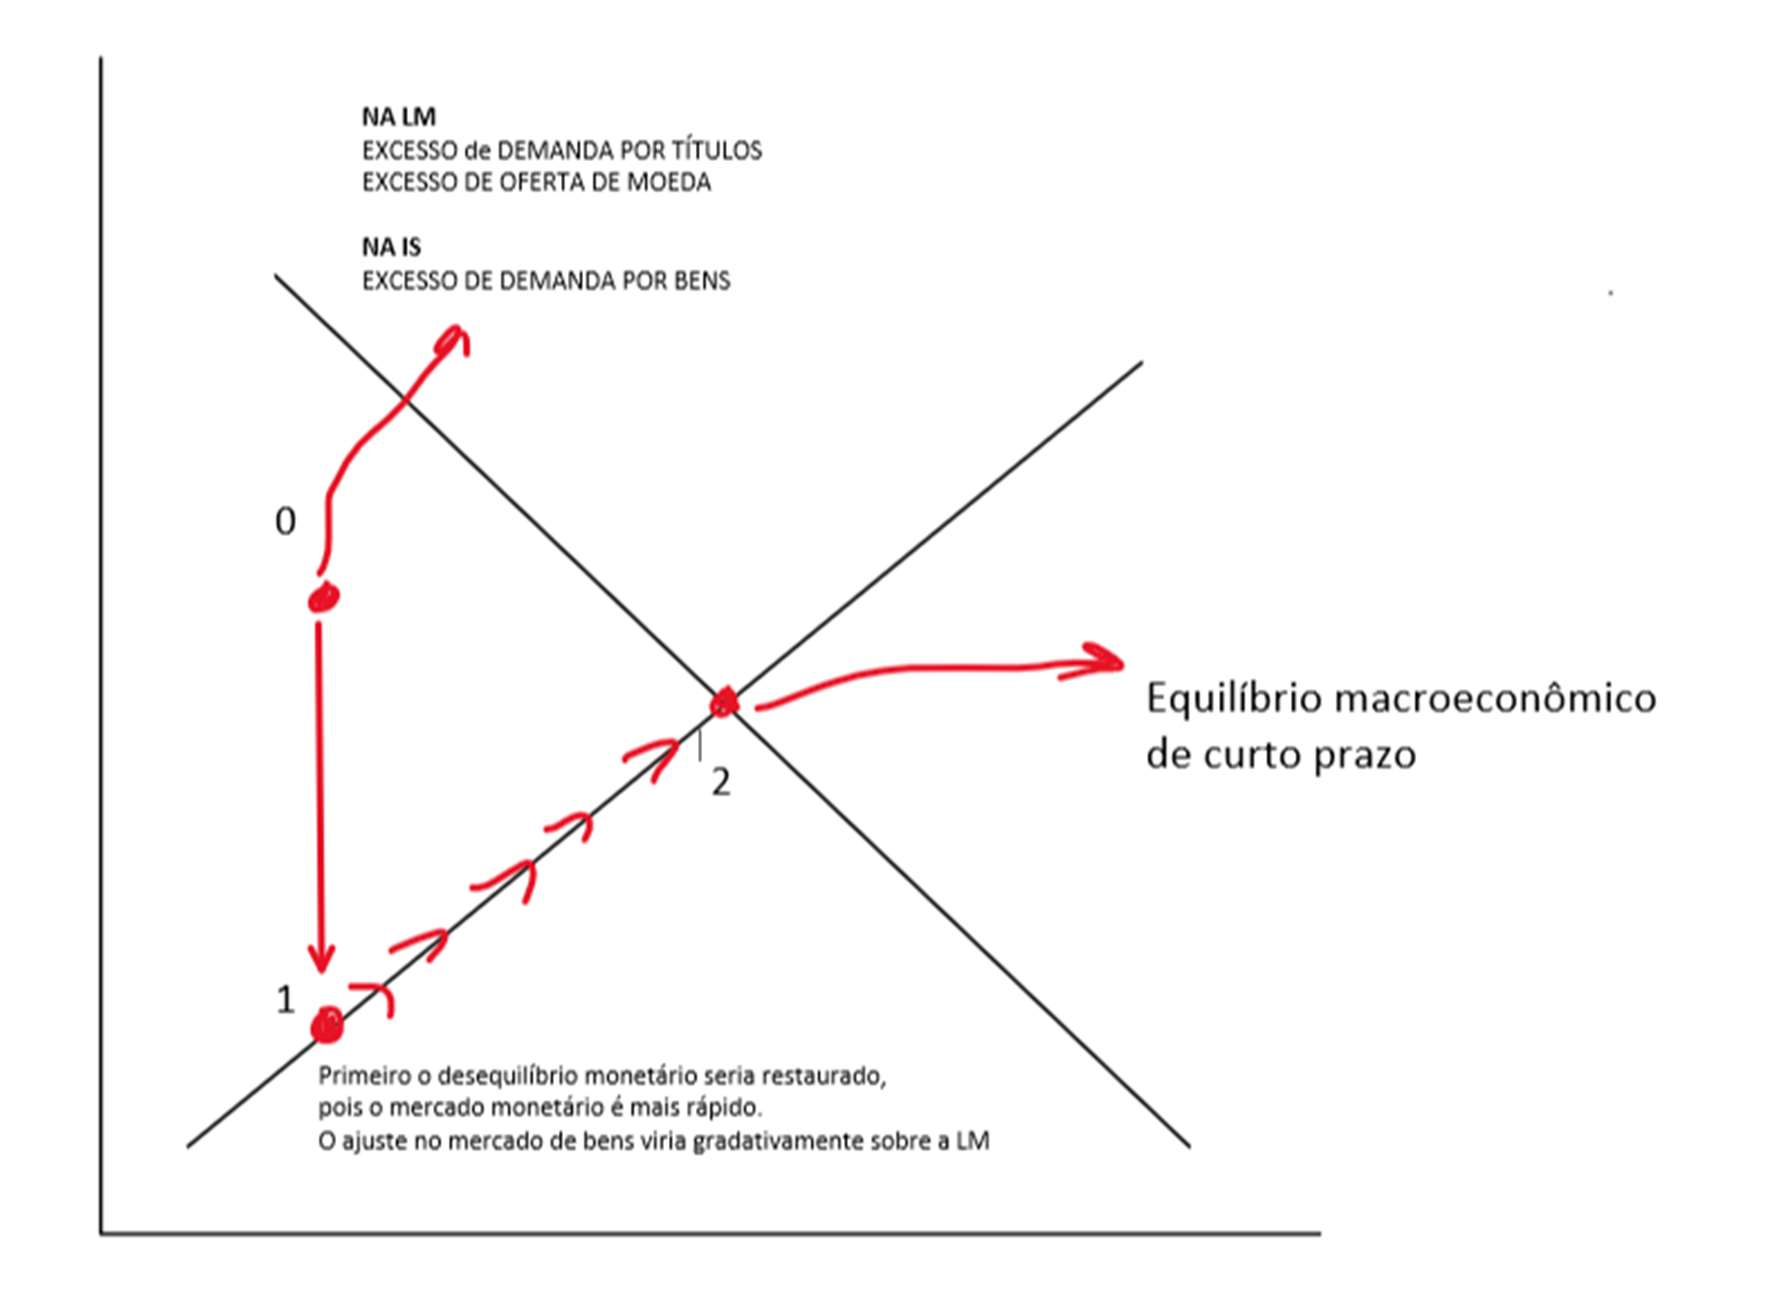
\includegraphics[width=0.7\linewidth]{Imagens/a4i2.png}
\end{figure}

\subsection{\textbf{Choques de Políticas}}
\textbf{Fiscal expansionista }\begin{itemize}
    \item $\Delta g>0$
    \item $\Delta t<0$
    \item $\Delta(g-t)>0$
    \item \textbf{Efeito deslocamento (crowding-out)}: Ocorre quando o governo aumenta os gastos públicos no intuito de expandir a economia, mas o efeito é anulado graças à elevação das taxas de juros e diminuição dos investimentos advindos do setor privado. A existência desse efeito é explicada a partir de uma diminuição dos fatores de consumo em uma economia. Ou seja, o crowding out acontece porque estes fatores de consumo são suscetíveis às taxas de juros quando há aumento das despesas do Estado. Assim, como o Estado passa a concorrer com as entidades privadas que também se financiam por meio dos mercados monetários, se tem o aumento das taxas de juros, devido ao aumento da busca por fundos. Por outro lado, o aumento da taxa de juros leva à diminuição do consumo privado e dos investimentos, visto que o financiamento se torna mais caro para as empresas. Neste contexto temos o crowding out, que provoca a redução do investimento e de outros componentes de despesa agregada que são influenciadas pelas taxas de juros. \textbf{Crowding-out}\begin{itemize}
        \item Situação macroeconômica que advém de gastos deficitários do governo. Ou seja, o governo gasta mais do que o necessário, sendo obrigado a emprestar o restante para cobrir o déficit
        \item Assim, as taxas de juros tendem a aumentar e isso acaba diminuindo os investimentos corporativos. Para levantar fundos, o governo vai emitir títulos que vão atrair a maioria dos poupadores de títulos privados.
        \item Desta forma, as instituições privadas sofrem uma redução no seu acesso às economias da economia.
    \end{itemize}
    \begin{figure}[H]
        \caption{Expansão fiscal e efeitos na IS-LM}
        \centering
        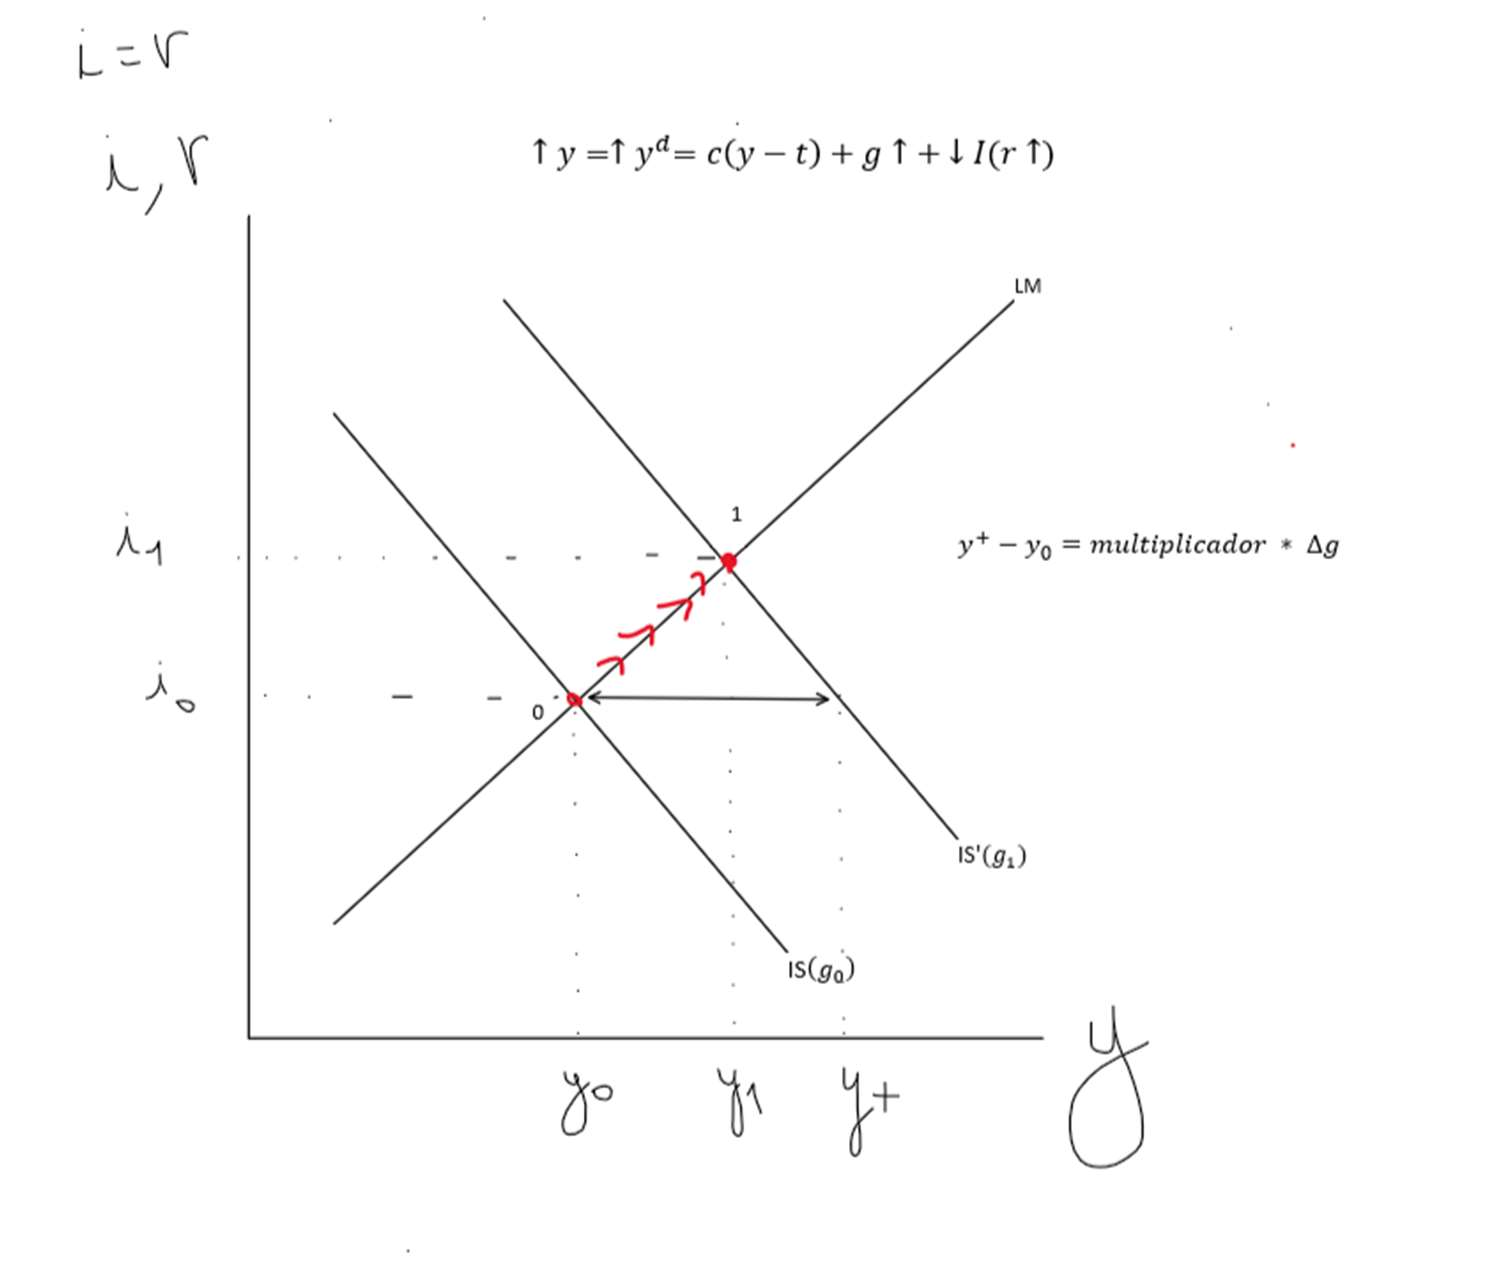
\includegraphics[width=0.7\linewidth]{Imagens/a4i3.png}
    \end{figure}
    \begin{figure}[H]
        \centering
        \caption{Expansão fiscal e efeitos na IS-LM}
        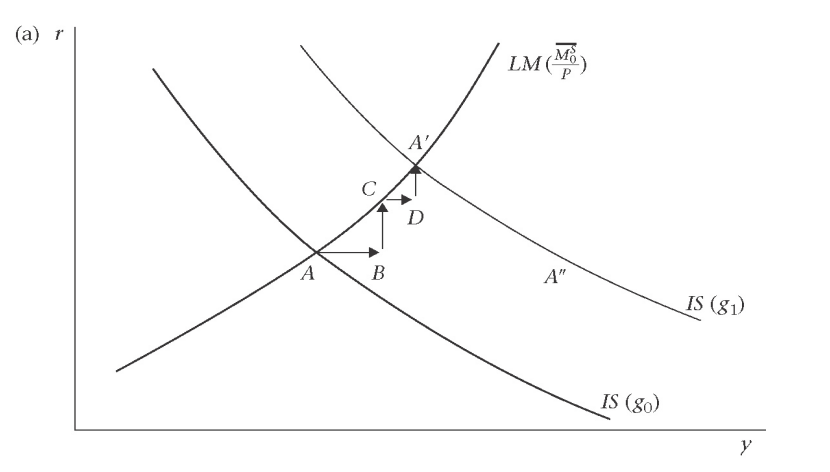
\includegraphics[width=0.7\linewidth]{Imagens/a4i7.png}
    \end{figure}
\end{itemize}

\textbf{Monetária expansionista }\begin{itemize}
    \item $\Delta M^s>0$
    \item Em um aumento da oferta monetária, o BACEN compra títulos, o que, por consequência afeta o equilíbrio no mercado de título, que torna a afetar taxa nominal de juros ($\downarrow i$) conforme os preços dos títulos sobem. $\frac{\uparrow M^s}{p}=l-l_i(\downarrow i)+\frac{y}{v_T}$
    \item  Dessa  forma,  a  diminuição  da  taxa  de  juros  impacta  gradativamente  a  demanda  por investimentos privados, que acelera a economia, estimulando a demanda e produto.$\downarrow r\rightarrow \uparrow I\rightarrow\uparrow y^d\rightarrow\uparrow y$
    \begin{figure}[H]
        \centering
        \caption{Expansão Monetária e efeitos na IS-LM}
        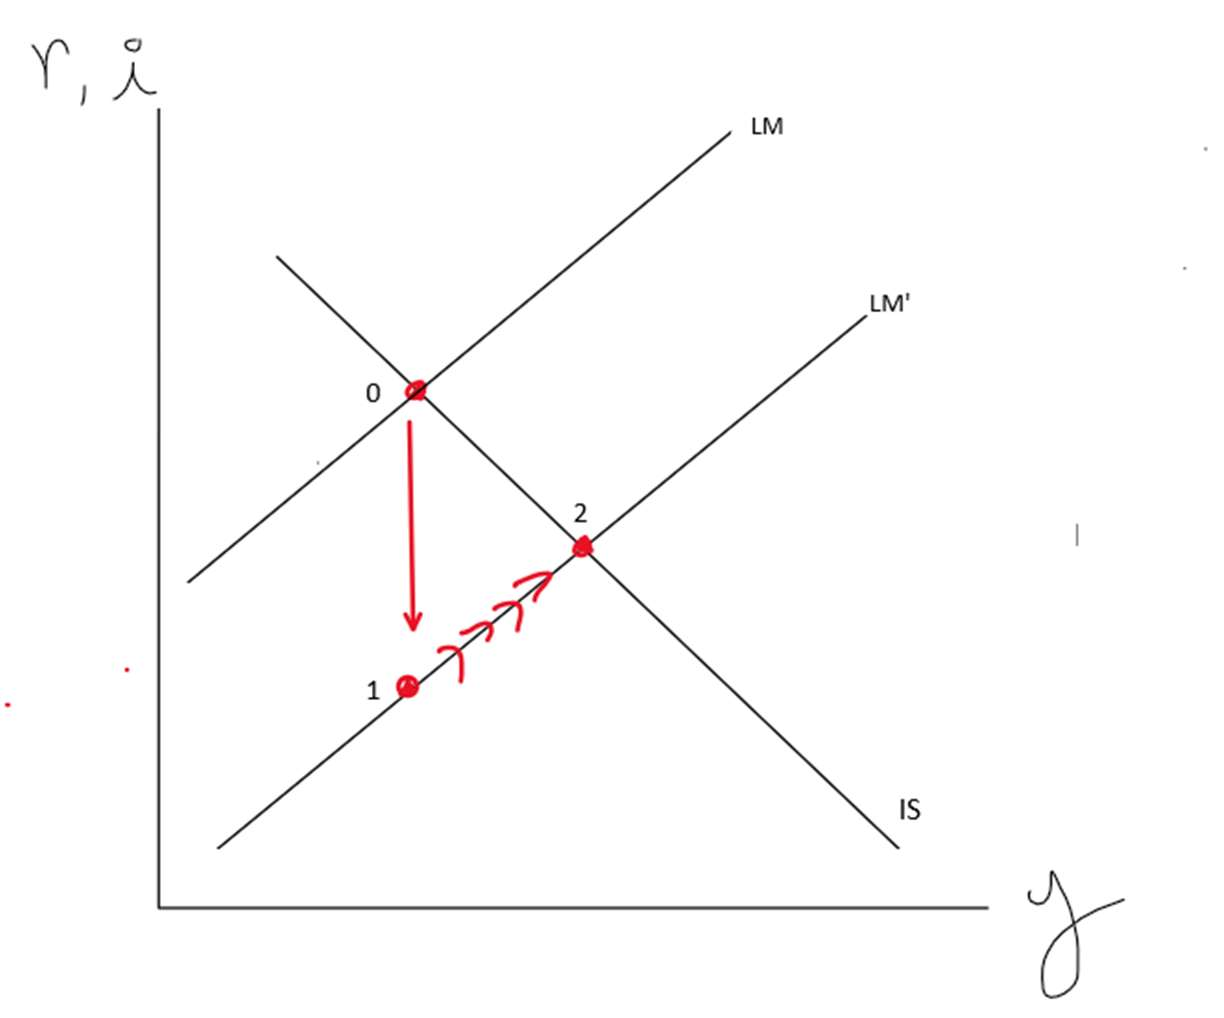
\includegraphics[width=0.7\linewidth]{Imagens/a4i4.png}
    \end{figure}
    \begin{figure}[H]
        \centering
        \caption{Expansão Monetária e efeitos na IS-LM}
        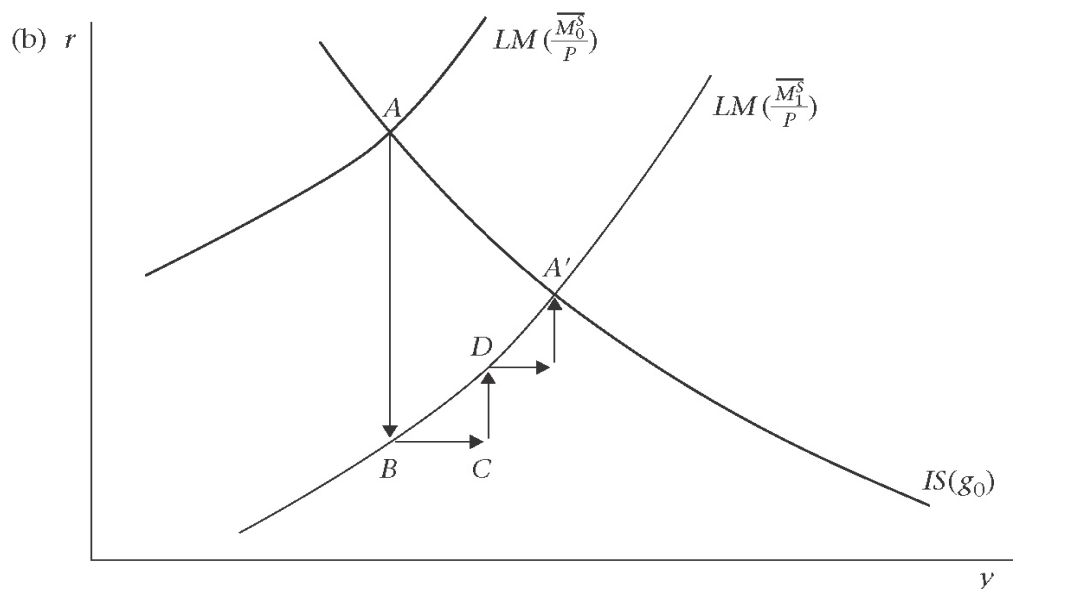
\includegraphics[width=0.7\linewidth]{Imagens/a4i8.png}
    \end{figure}
\end{itemize}

\subsection{\textbf{Armadilha da Liquidez}}
Considere um choque negativo de demanda que cause uma grande recessão, ou mesmo depressão:
\( \downarrow\downarrow y^d \to \downarrow\downarrow y < y_e \to \textit{deflação} \)

Nesse contexto, a política mais tradicional para se estabilizar o produto é a realização de uma política monetária expansionista, partindo de uma compra de títulos que contrai a taxa de juros nominal:
\( \uparrow M^S \to \downarrow i \to \downarrow r, \quad \text{na restrição de que } i \geq 0. \)

Assim, nasce o cenário de \textbf{Armadilha de Liquidez}: quando a taxa nominal de juros está muito próxima de zero, ou literalmente igual a zero, e o consumo e produção estiverem em grande recessão. Assim, nesse contexto:
\( i = 0 \to r = 0 - \pi, \quad \uparrow r = \downarrow \pi, \)
retroalimentação da deflação. A crescente taxa \textbf{REAL} de juros contribui para a contração adicional do produto, estimulando a deflação.

É evidente que uma taxa de juros muito baixa não significa que existem poucos títulos em circulação no mercado. Em um cenário de incerteza como uma depressão, existe uma percepção de risco que pode tornar mais atraente manter ativos facilmente liquidados, que garantem menor risco, do que manter o dinheiro na conta corrente nos bancos, dada a possibilidade de que esses bancos possam quebrar.

Como a taxa nominal de juros é zero, moeda e títulos se tornam substitutos muito próximos, tornando as \textbf{políticas monetárias convencionais inefetivas}. Isso, pois a injeção de liquidez a partir da compra de títulos não afetaria os preços dos mesmos, uma vez que a moeda seria retida na sua forma líquida, não alterando a taxa nominal de juros e, portanto, sendo inefetiva em aproximar o produto contraído ao produto de pleno emprego.

\begin{figure}[H]
    \centering
    \caption{Representação da LM Horizontal devido a Armadilha da Liquidez}
    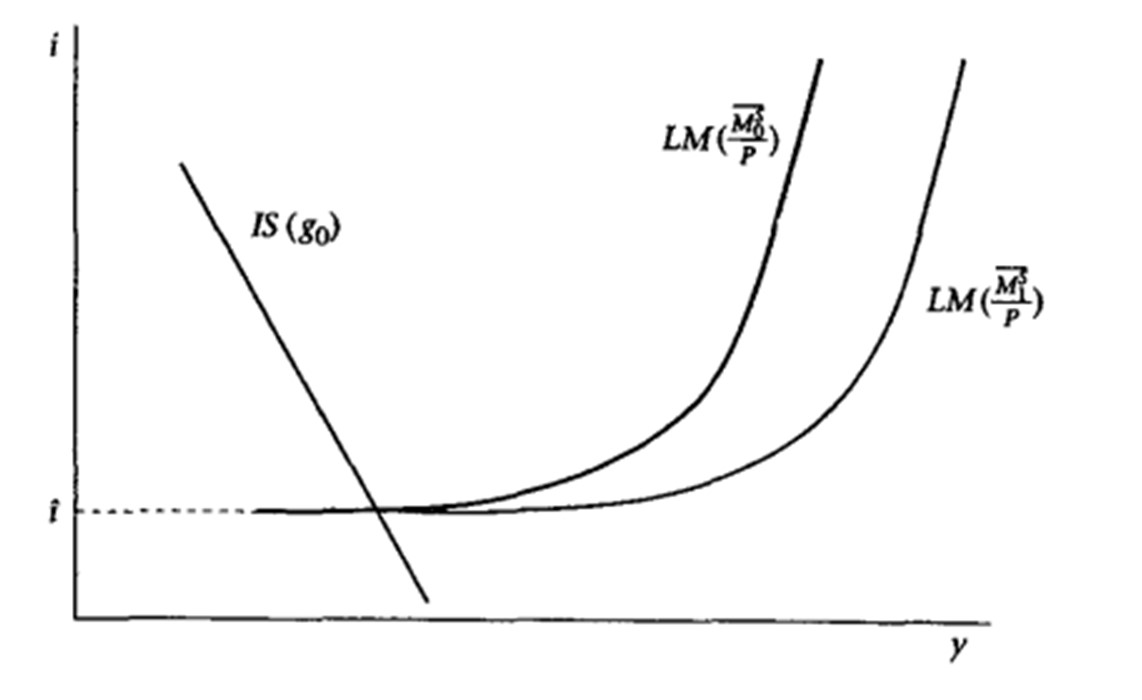
\includegraphics[width=0.7\linewidth]{Imagens/a4i5.png}
\end{figure}

\subsubsection{\textbf{Soluções para sair dessa situação}}
\textbf{Política Fiscal}:Realizar uma política fiscal pode, se realizada de forma bem planejada, contribuir para se aproximar o nível de produto até então contraído ao nível de produto de pleno emprego desejado. Observe que, em uma armadilha de liquidez, o crowding- out não existirá. 
\begin{figure}[H]
    \centering
    \caption{Representação da LM Horizontal devido a Armadilha da Liquidez com solução de expansão fiscal}
    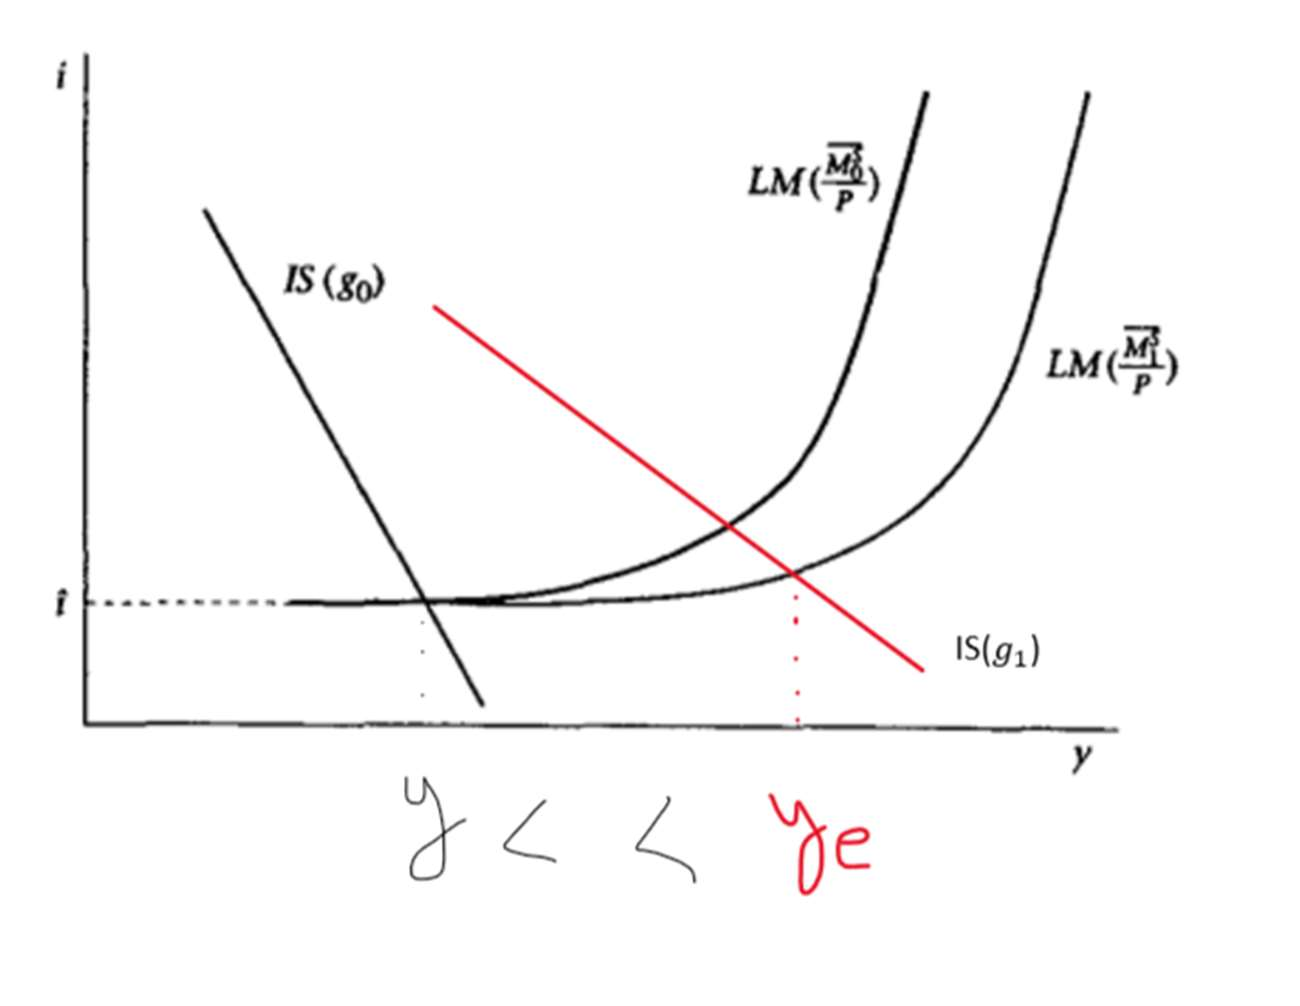
\includegraphics[width=0.7\linewidth]{Imagens/a4i6.png}
\end{figure}

\textbf{Política monetária não convencional}:Quando realizada uma política monetária NÃO CONVENCIONAL, como o BACEN buscar atuar sobre a inflação esperada, elevando-a, pode-se sim obter efeitos no produto, apesar do contexto de armadilha de liquidez. Injetando liquidez abundante e se comprometendo a não a contrair quando a inflação subir pode ter efeito na relação de $r=-\pi$ vista na armadilha de liquidez, com o efeito de $\uparrow \pi \rightarrow \downarrow r \rightarrow \uparrow y^d \rightarrow \uparrow y$

\subsection{\textbf{Oferta agregada: mercado competitivo}}
A função de produção relaciona o volume de emprego $E$ ao nível de produto y através de \(y=f(E:emprego,\underbrace{K:capital, tecnologia, energia,etc}_{cte})\) a função de produção \(f(\cdot)\). Toma tecnologia e o estoque de capital como dados no curto médio prazo. Além disso, apresenta retornos decrescente(quanto maior o nível de emprego, maior a produção mas a taxas decrescentes).


\begin{itemize}
    \item \textbf{Oferta:} A função de produção é dada por:
    \[
    y = f(E, \text{capital, tecnologia, etc.})
    \]
    onde $E$ representa o emprego.

    \item \textbf{Fluxo de Produção:}
    \[
    y = \underbrace{\lambda}_{produtividade} E^{\theta}, \quad 0 < \theta < 1
    \]

    \item \textbf{Retornos Decrescentes:} As condições para retornos decrescentes são:
    \[
    \frac{\partial f}{\partial E}=\underbrace{\lambda\theta E^{\theta-1}}_{\text{produtividade marginal do trabalho}} > 0, \quad \frac{\partial^2 f}{\partial E^2}=\lambda\theta(\theta -1) E^{\theta-2} < 0
    \]
    \begin{figure}[H]
        \centering
        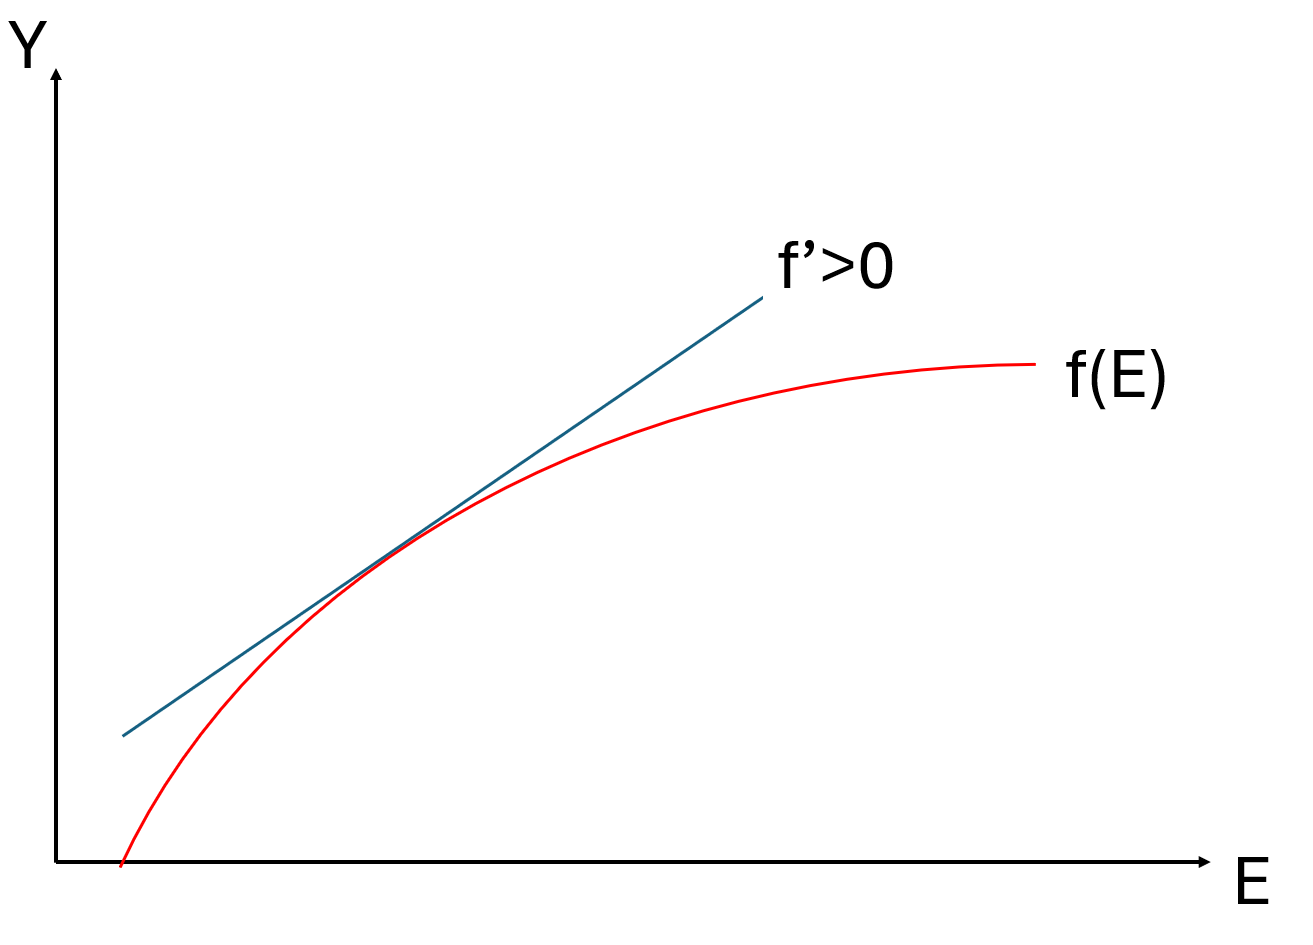
\includegraphics[width=0.7\linewidth]{Imagens/a5i2.png}
    \end{figure}

    \begin{figure}[H]
        \centering
        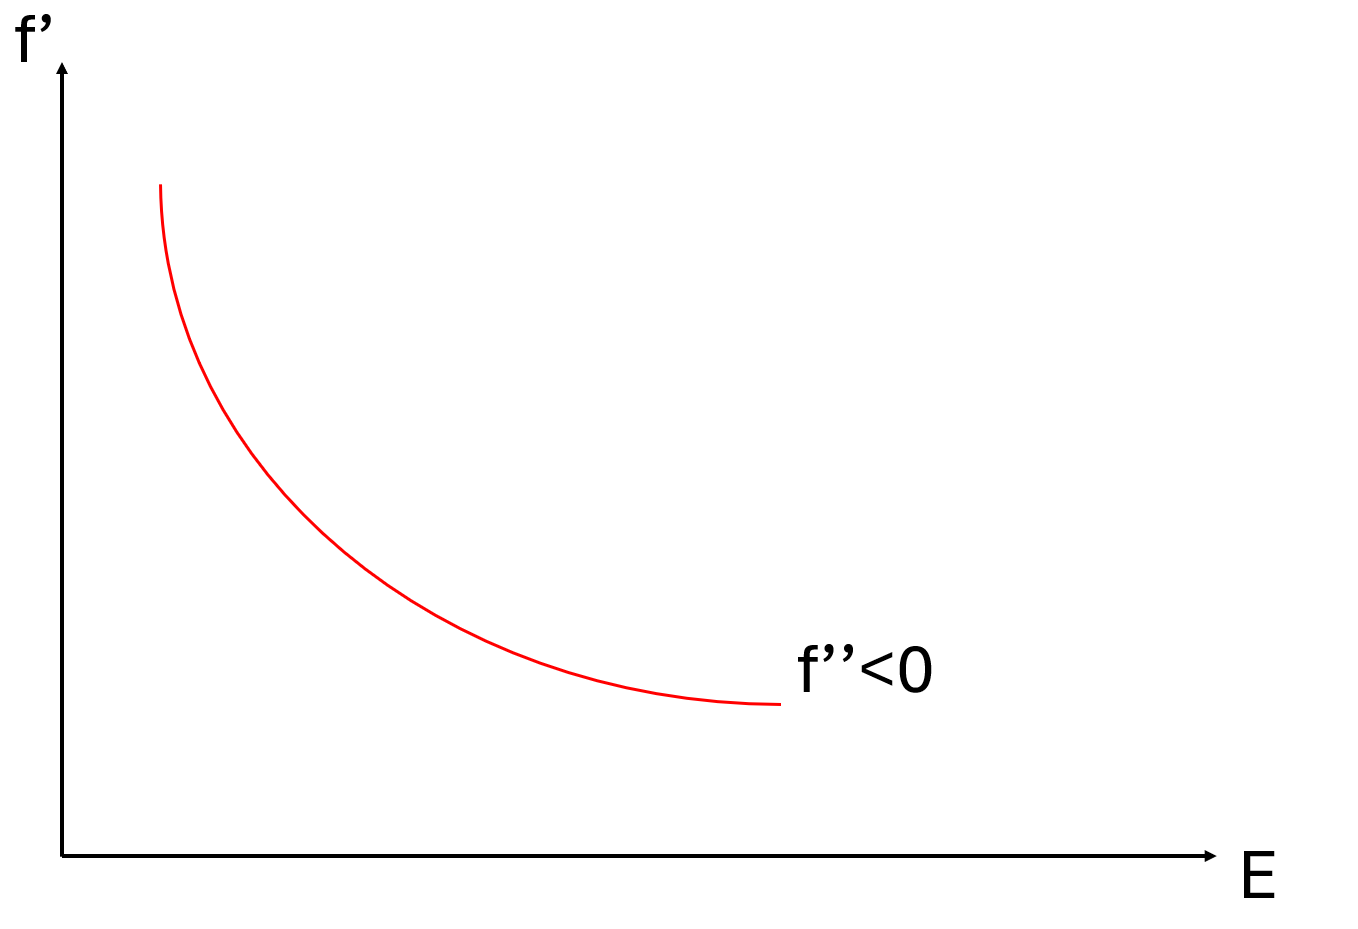
\includegraphics[width=0.7\linewidth]{Imagens/a5i3.png}
    \end{figure}
    
\end{itemize}

Podemos definir que a função de produção possuí retornos constantes de escala, sendo assim \(\theta =1\), senda definida por :
\[
y=\lambda E
\]

\[
\frac{\partial f}{\partial E}=\underbrace{\lambda E}_{\text{produtividade marginal do trabalho}} =\frac{y}{E}, \quad \frac{\partial^2 f}{\partial E^2}=0
\]

\begin{figure}[H]
    \centering
    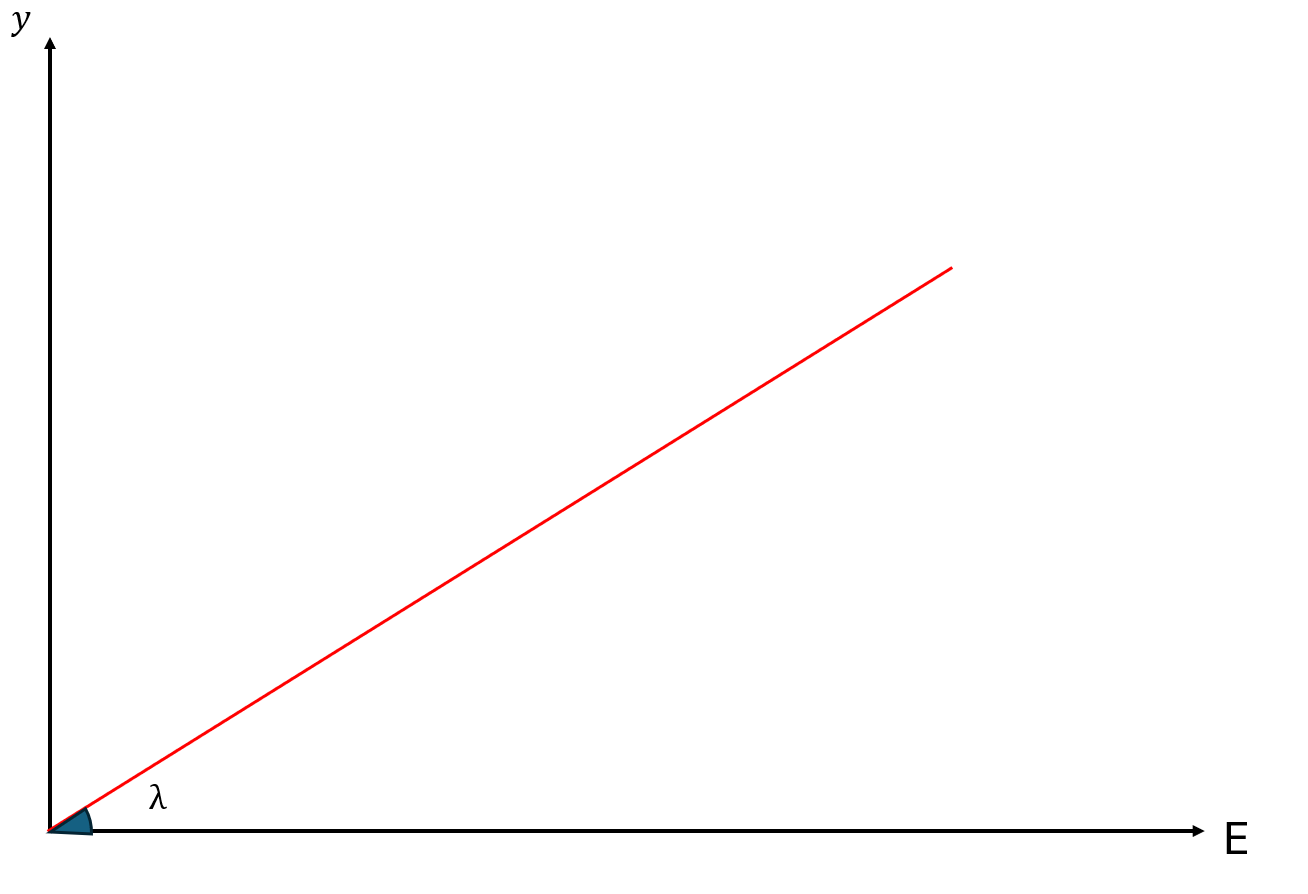
\includegraphics[width=0.7\linewidth]{Imagens/a5i10.png}
\end{figure}

\begin{figure}[H]
    \centering
    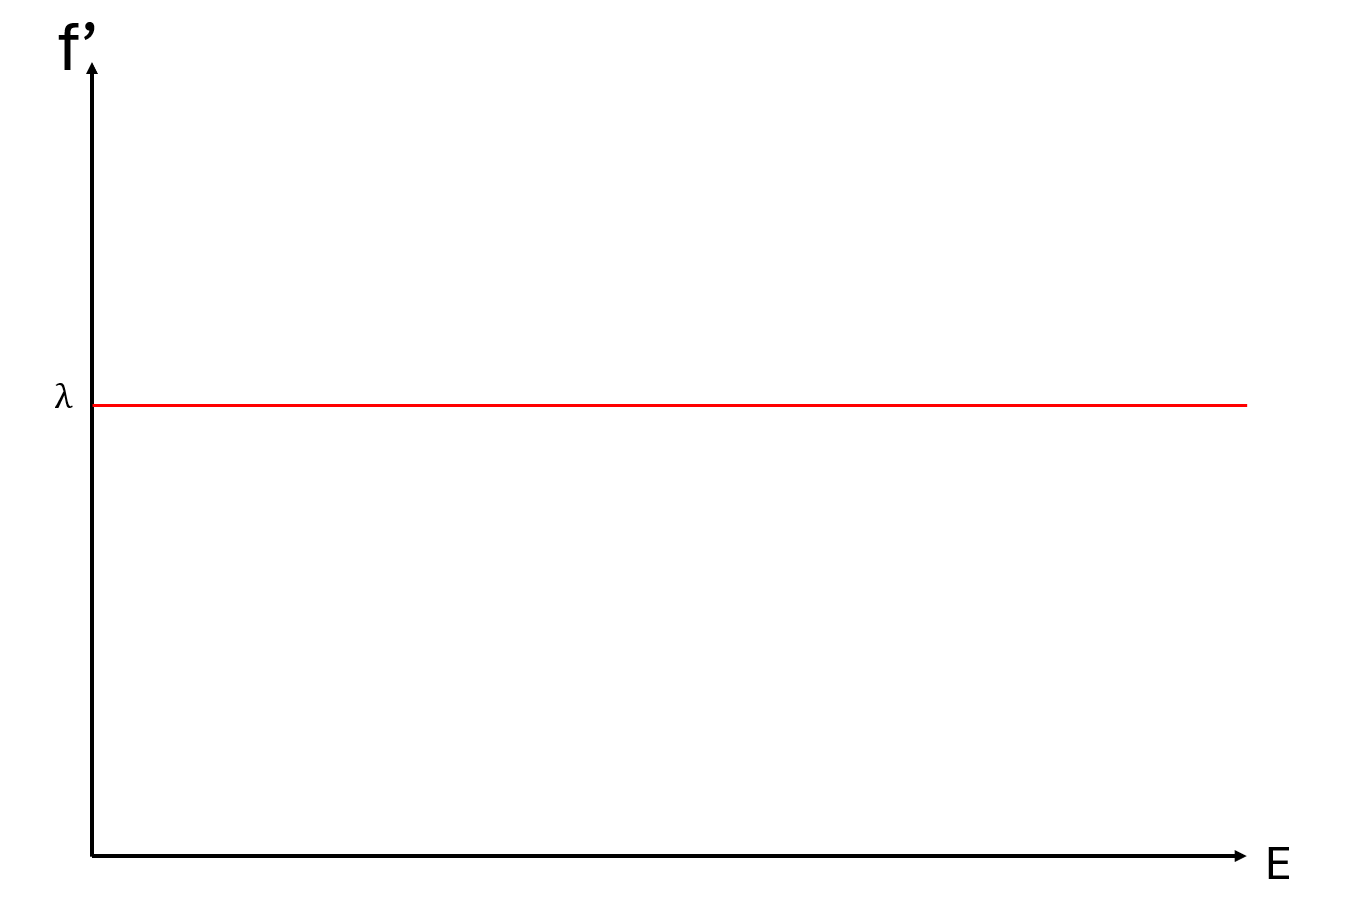
\includegraphics[width=0.7\linewidth]{Imagens/a5i11.png}
\end{figure}

A função de demanda por trabalho\(E^D\), ela resulta da decisão de maximização de lucros pelas empresas. Além disso, reflete a escolha ótima de emprego do trabalho para cada nível do salário real e por fim ela é uma função decrescente do salário real, refletindo a produtividade marginal decrescente.

A função de oferta de trabalho, $E^S$, ela resulta da decisão de maximização de utilidade individual. Além disso, ela reflete a escolha ótima de tempo entre lazer e trabalho para cada nível do salário real, por fim ela é uma função decrescente do salário real. Empresas e a população são tomadores de preços e salários, tendendo ao nível de salários reais de \textit{Market Clearing}.

Antes de tudo, definimos a função de lucros de uma empresa:
\[
Lucro = P\cdot y-W\cdot E=P\cdot f(E)-W\cdot E
\]

Derivando lucro em relação a variações em emprego:
\[
\max_{E} \ Lucro=P \cdot f'(E) - W=0
\]

Perceba que: \begin{itemize}
    \item \(P \cdot f'(E)\) é a receita marginal dessa empresa (\(R_{mg}\))
    \item W é o custo marginal dessa empresa (\(C_{mg}\))
\end{itemize}

Assim, tem-se que a produtividade marginal do trabalhador será \(f'(E)\) e que o preço se dá por \(P=\frac{W}{f'(E)}\). Portanto, salário real será dado por \(\frac{W}{p}=f'(E^d)\), sendo que \(E^d\)(função de produtividade marginal do trabalho) é a curva de demanda por trabalhado que expressa os níveis de reais de salário demandado para cada nível de emprego.

\begin{figure}[H]
    \centering
    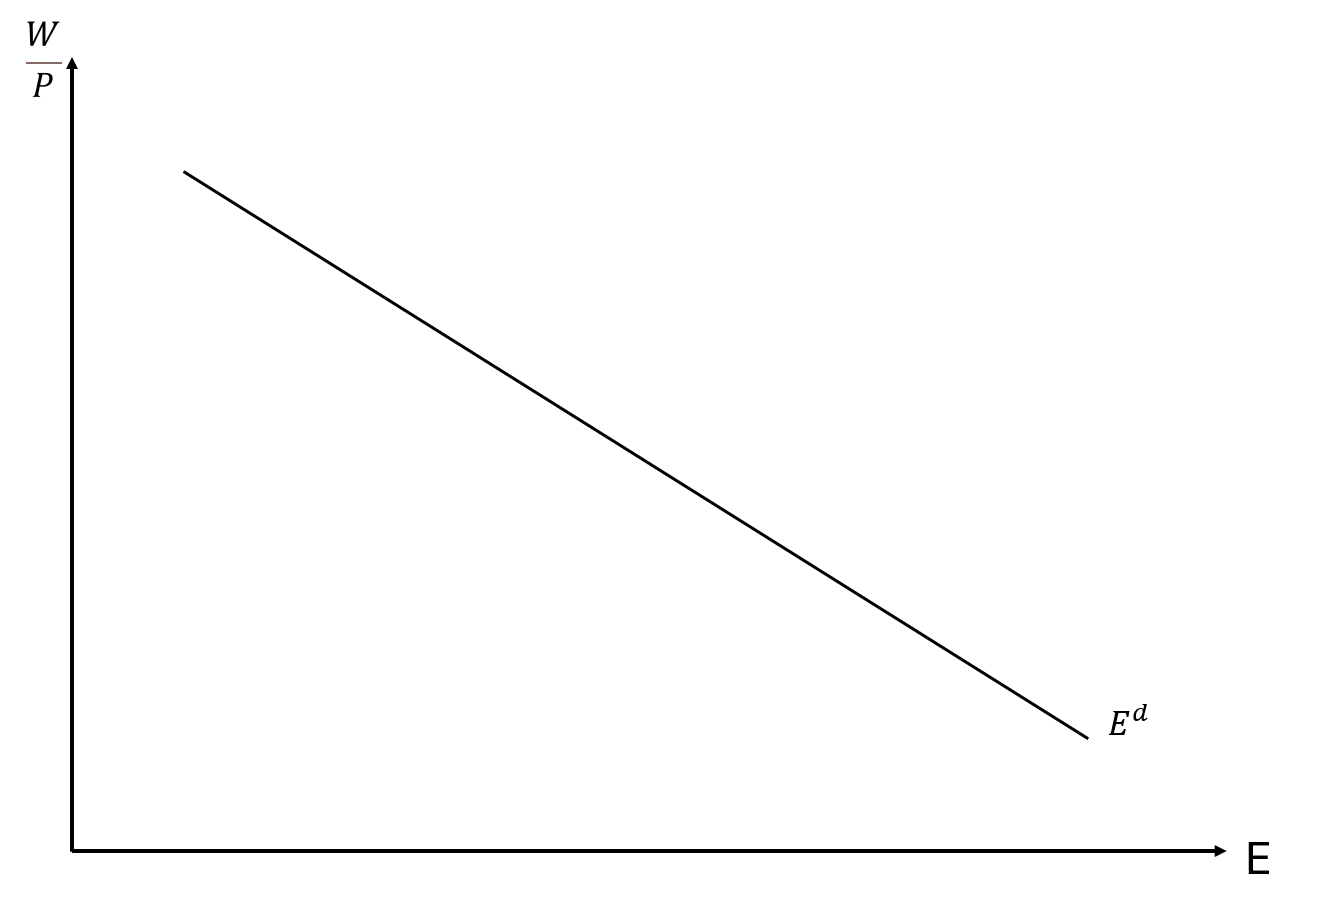
\includegraphics[width=0.7\linewidth]{Imagens/a5i4.png}
\end{figure}

\begin{figure}[H]
    \centering
    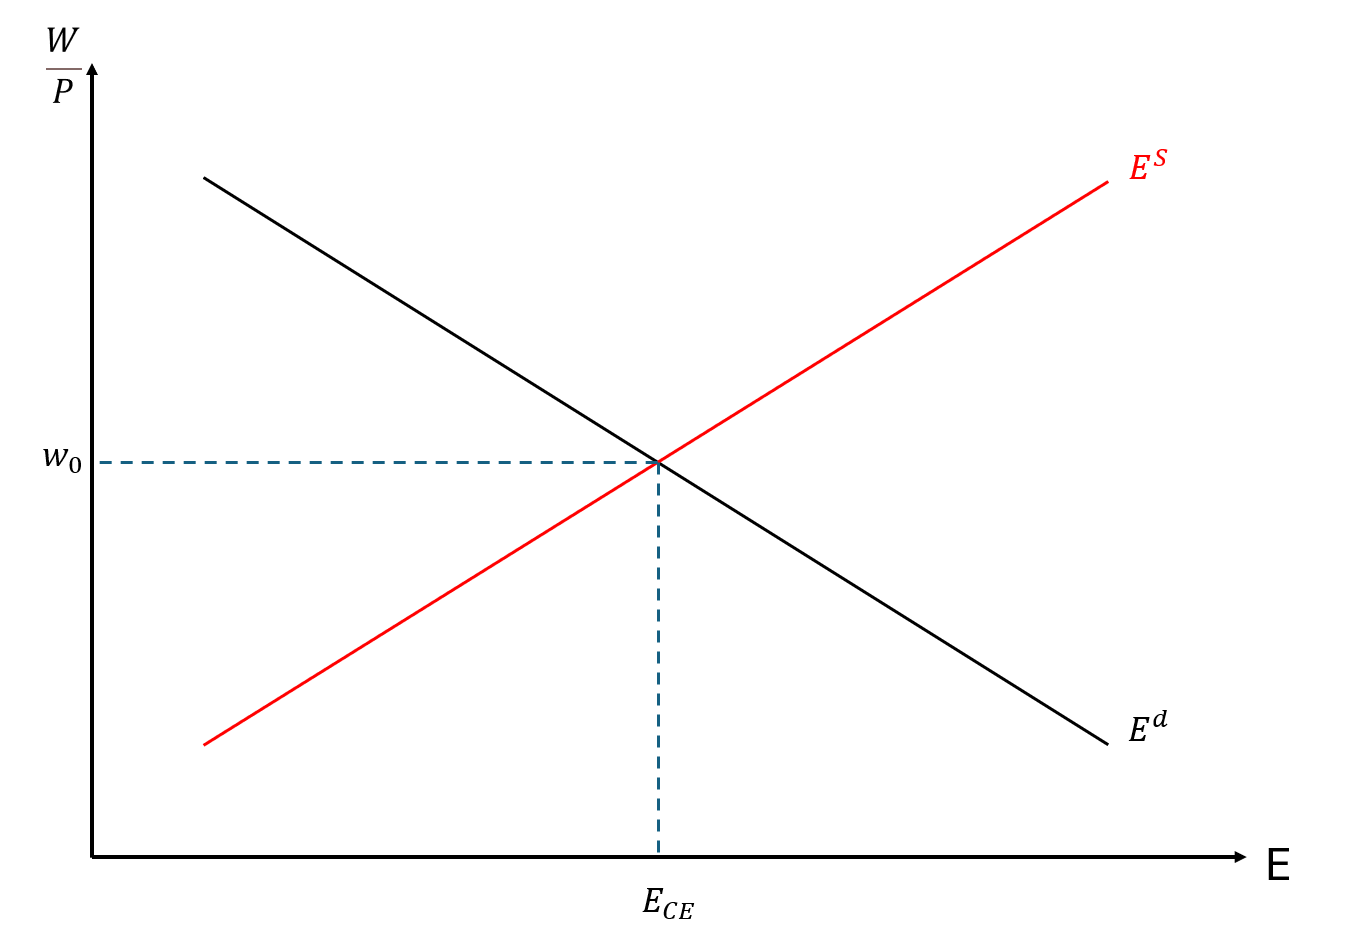
\includegraphics[width=0.7\linewidth]{Imagens/a5i5.png}
\end{figure}

\begin{figure}[H]
    \centering
    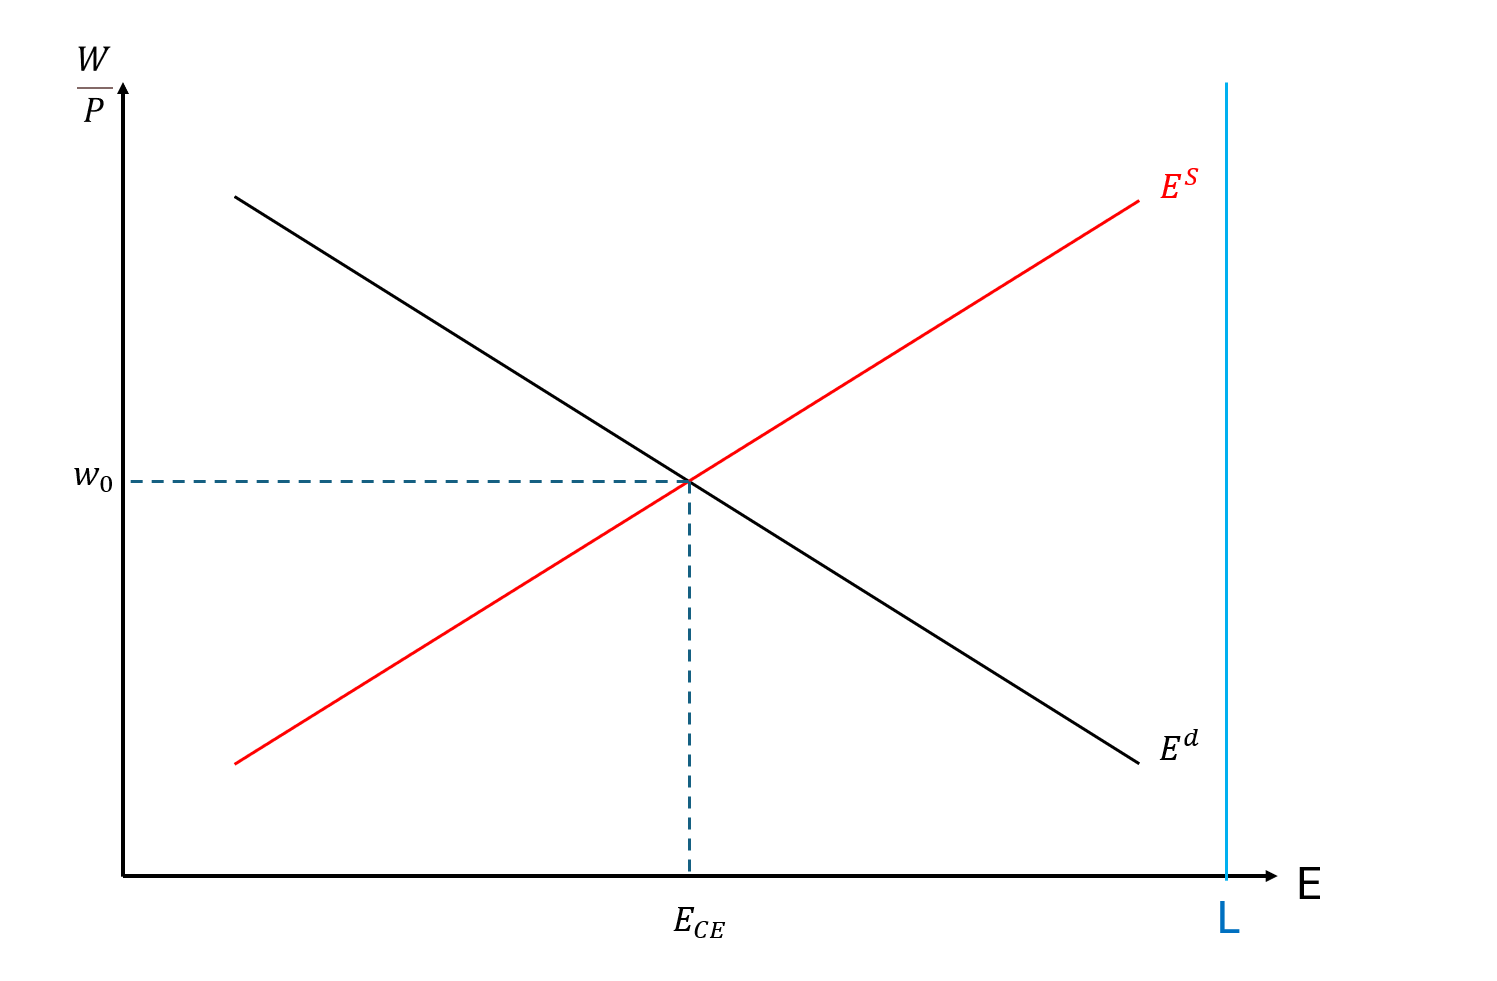
\includegraphics[width=0.7\linewidth]{Imagens/a5i6.png}
\end{figure}

Onde \(E^S\)(reflete o custo de oportunidade da renúncia ao lazer para maior consumo) é a \textbf{oferta de empregos em um mercado competitivo perfeito}. \(E_{CE}\) é o \textbf{nível de emprego no equilíbrio competitivo perfeito}. \(L\) é o \textbf{tamanho da força de trabalho disponível nesse economia}(\(L=E_{CE}+U_{CE}\)). \(U_{CE}\) é o \textbf{nível de desemprego no equilíbrio competitivo perfeito}.

Com mercados competitivos, oferta e demanda se encontravam, estabelecendo o salário real \(w_0\) e o nível de emprego \(E_{CE}\) associados ao equilíbrio competitivo.

\begin{figure}[H]
    \centering
    \caption{Representação do Mercado de Trabalho}
    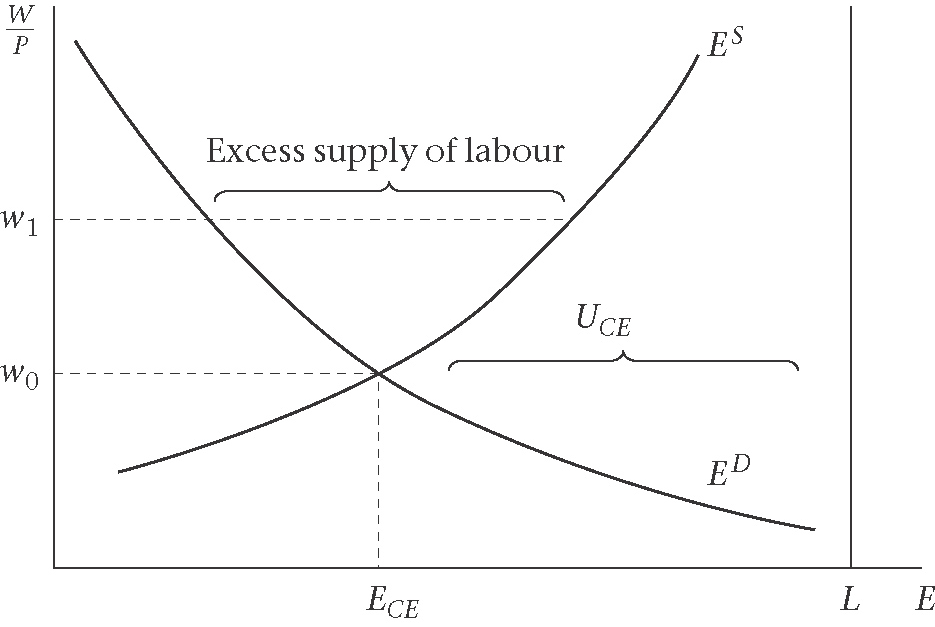
\includegraphics[width=0.7\linewidth]{Imagens/a5i1.png}
\end{figure}

\[
\frac{W}{P}=\lambda\theta E^{\theta-1}=f'(E)\rightarrow (\frac{1}{\lambda\theta}\frac{W}{P})^{\frac{1}{\theta-1}}=E^d
\]

Observações importantes:\begin{itemize}
    \item Num mercado de trabalho competitivo qualquer descompasso entre oferta e demanda é eliminado por alterações no salário.
    \item Eventual desemprego é voluntário: ao salário real corrente, trabalhadores preferem desfrutar de lazer ou procurar emprego ao fluxo de renda obtido através do trabalho.
    \item A força de trabalho máxima que poderia ser ofertado é a soma dos empregos e dos desempregado \(L=E_{CE}+U_{CE}\).
    \item Uma taxa de desemprego \(U_{CE}/L>0\) reflete decisões individuais ótimas e não representam uma diminuição de do bem-estar.
\end{itemize}

Se eventualmente houver algum nível de oferta de trabalhadores em excesso (\(E^d<E^S\)), é evidente como se os salários que até estavam em \(w^+\) ficaram exagerados para toda essa oferta de trabalhadores que estariam dispostos a trabalhar por menos. Assim, o excesso tornaria os salários ofertados gradualmente mais baixos, até que, com o tempo, se retorne ao nível de emprego de equilíbrio competitivo perfeito.
\begin{figure}[H]
    \centering
    \caption{Desiquilíbrios no mercado de trabalho.}
    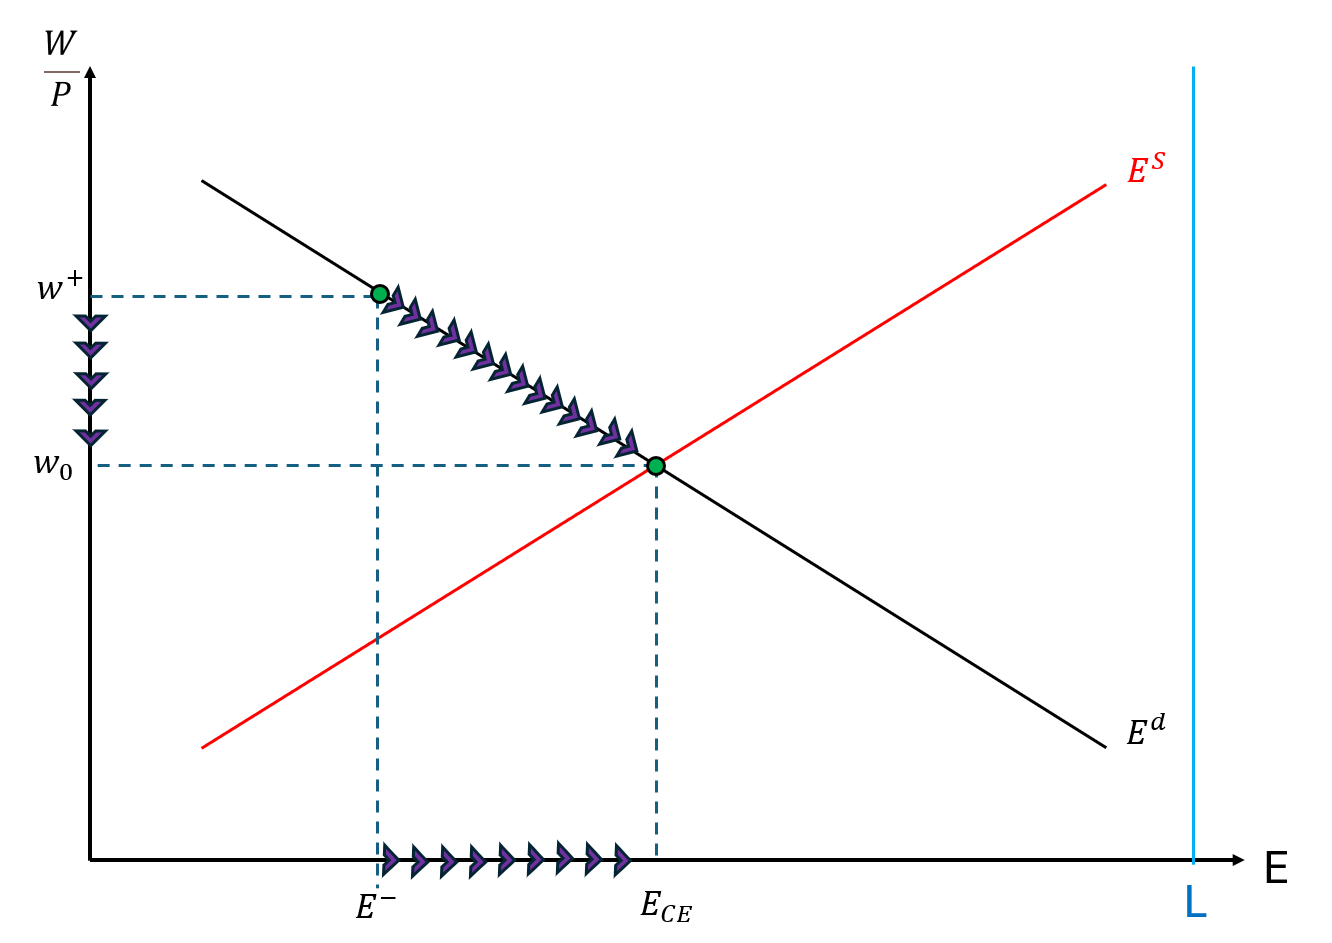
\includegraphics[width=0.7\linewidth]{Imagens/a5i7.png}
\end{figure}

\subsection{\textbf{Oferta agregada: concorrência imperfeita}}

Paradigma do mercado competitivo não é muito realista: trabalho, em geral, não é competitivo e vendido em mercados spot:\begin{itemize}
    \item há negociações coletivas e sindicatos
    \item há contratos e regulações
    \item há necessidade de motivar os trabalhadores para empregarem o nível eficiente de esforço
\end{itemize}

Empresas operando sob concorrência imperfeita no mercado de produtos estabelecem uma margem sobre os custos para determinar o preço final dos bens. O salário real depende de decisões de salários e preços de toda economia. 

\subsection{\textbf{Salários}}
Sob concorrência imperfeito e com imperfeições no mercado de trabalho: \begin{itemize}
    \item a oferta de emprego é a menor do que sob condições competitivas
    \item o salário demandado é maior do que sob condições competitivas
    \item há \textit{mark-up} sobre salário do equilíbrio competitivo
\end{itemize}

A curva de oferta de trabalho ou demanda por salários com poder de mercado, \textbf{WS}(\textit{wage-setters}), segue \(W=P^e\cdot b(E)\), com a função \(b(E) \ \  ;\  b'(E)>0\) crescente em \(E\) refletindo tanto o poder de barganha dos trabalhadores como o pagamento de salários-eficiência pelas empresas(lembrando que \(E^S\) é a oferta de trabalho sobre concorrência perfeita).

\begin{figure}[H]
    \centering
    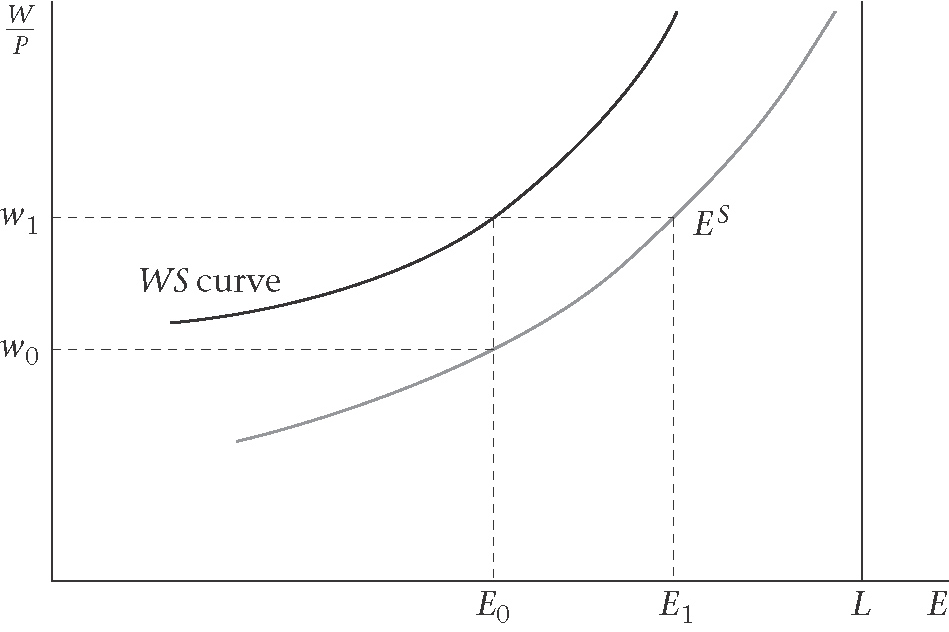
\includegraphics[width=0.7\linewidth]{Imagens/a5i8.png}
\end{figure}

Apesar de negociarem salários nominais trabalhadores se preocuparem com a remuneração real esperada: portanto, a fixação do salário real segue \(w^{WS}\equiv \frac{W}{P}=b(E)\), quando o nível de preços esperado e efetivo são idênticos.

Sendo, \(W\) o salário nominal negociado pelos fixadores de salário(\textit{wage-setters}; \(P^e\)), o nível de preços esperado; e \(b(E)\) é a função que expressa o poder de barganha dos trabalhadores\((b'(E))>0\). Assim, quando \(P^e=P\), é possível definir a função WS:
\[
w^{WS}=(\frac{W}{P})^{WS}=b(E)
\]

\begin{figure}[H]
    \centering
    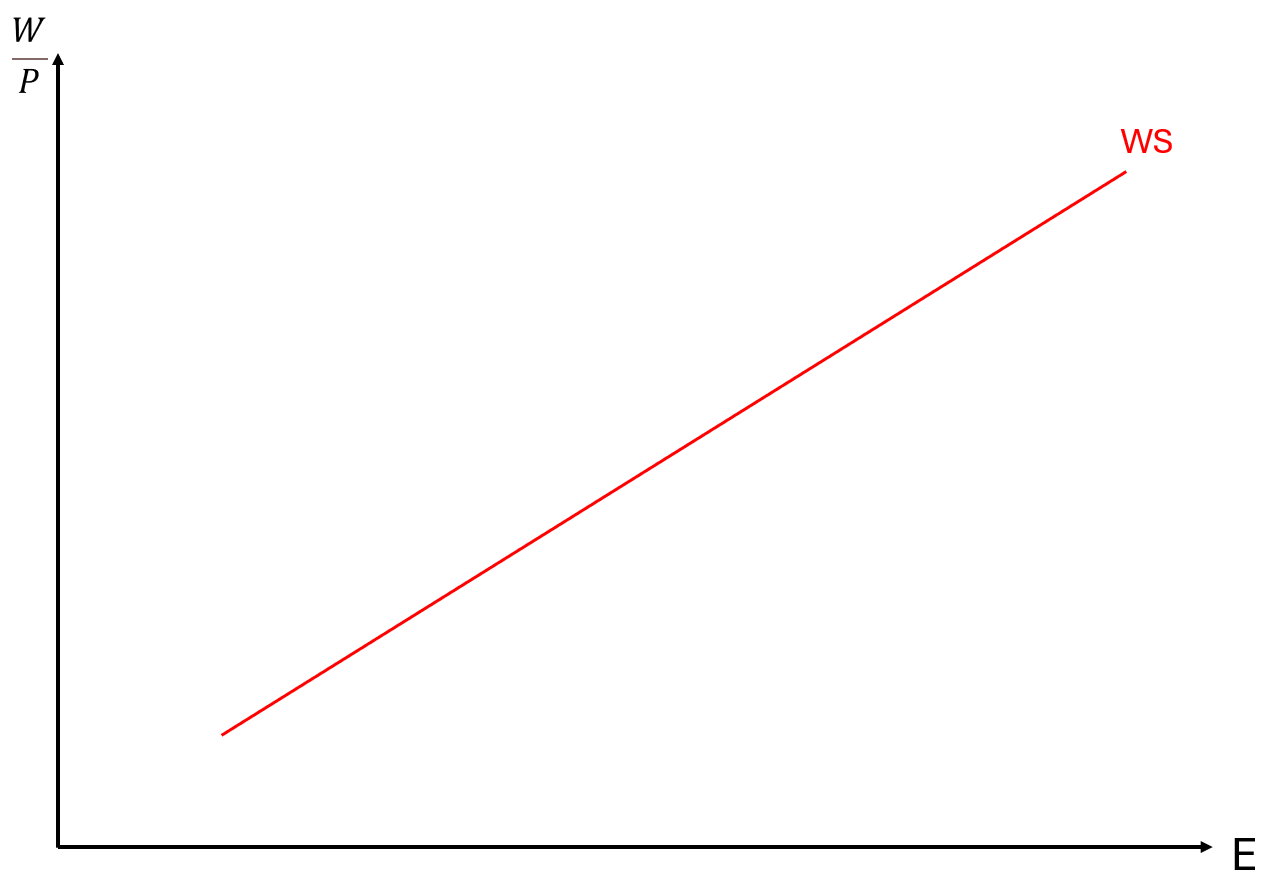
\includegraphics[width=0.7\linewidth]{Imagens/a5i9.png}
\end{figure}

\subsection{\textbf{Preços}}
Sob concorrência perfeita o preço reflete o custo marginal, custo marginal = receita marginal = P:
\[
P=MC=\frac{W}{MPL}\rightarrow\frac{W}{P}=MPL
\]

A remuneração do trabalho reflete sua produtividade marginal, a formação de preços sob concorrência monopolística: custo marginal = receita marginal < P

Como as empresas se comportam no processo de fixação de preços e escolha do nível de emprego para encontrar a maximização dos lucros em um mercado competitivo imperfeito? 

\textbf{Elasticidade preço da demanda}  \(\rightarrow\)É a sensibilidade da quantidade demandada por bens e serviços a oscilações nos preços. Define-se por: 

\[
\epsilon=-\frac{\frac{dy}{y}}{\frac{dP}{P}}
\]

Observe que a seguinte função de demanda:
\[
y=P^{-\epsilon} \rightarrow log(y)=-\epsilon\cdot log(P) \rightarrow \frac{1}{y}dy=-\epsilon \cdot \frac{1}{P}dP \rightarrow -\epsilon=\frac{\frac{dy}{y}}{\frac{dP}{P}}
\]

Foi assim que se encontrou a relação da elasticidade constante partindo da relação entre produto e preço acima. Agora, observe como se opera a equação para que se possa avaliar a função de maximização do lucro: 
\[ y = P^{-\varepsilon} \Rightarrow y^{\frac{1}{\varepsilon}} = f(E)^{\frac{1}{\varepsilon}} = P \]
(elevaram-se ambos os lados a \( \left(-\frac{1}{\varepsilon} \right) \)).

Agora substituindo na função de maximização dos lucros da firma:

\[
\max lucro_{(E)} = P \cdot y - W \cdot E
\]
\[
y^{\frac{1}{\varepsilon}} = \frac{\varepsilon}{\varepsilon} y^{\varepsilon} - W \cdot E
\]
\[
\max lucro_{(E)} = f(E)^{\frac{\varepsilon -1}{\varepsilon}} - W \cdot E
\]

Em seguida, deriva-se a função agora atrelada à elasticidade preço da demanda:
\[
\frac{\varepsilon - 1}{\varepsilon} \cdot f(E)^{\left(\frac{\varepsilon - 1}{\varepsilon}\right)} \cdot f'(E) - W= 0
\]
\[
\frac{\varepsilon - 1}{\varepsilon} \cdot f(E)^{\frac{1}{\varepsilon}} \cdot f'(E) = W
\]
\[
\underbrace{\left(\frac{\varepsilon - 1}{\varepsilon} \right) \cdot P \cdot f'(E)}_\text{Receita marginal} = \underbrace{W}_\text{Custo marginal}
\]

Note que \(\frac{\epsilon}{\epsilon-1}<1\), já que \(1<\epsilon<\infty\)

\(P^{PS}\) é o nível de preços que satisfaz as empresas(fixadoras de preços=\textit{picre-setters}):
\[
P^{PS}=\frac{\epsilon}{\epsilon-1}\cdot f'(E)=\frac{\epsilon}{\epsilon-1}\cdot MPL \rightarrow MPL>\frac{W}{P}
\]
\begin{figure}[H]
    \centering
    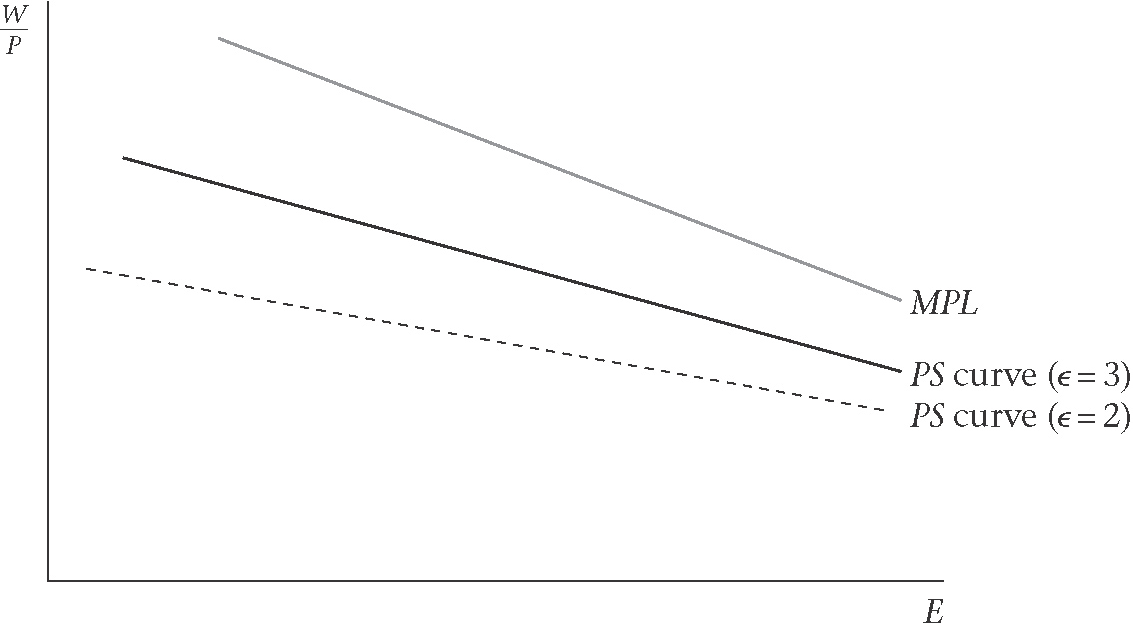
\includegraphics[width=0.7\linewidth]{Imagens/a5i12.png}
\end{figure}

A curva PS será horizontal quando:\begin{itemize}
    \item A produtividade marginal do trabalho (\textbf{MPL}) for constante.
    \item produtividade marginal do trabalho for decrescente mas a margem for contra-cíclica
    \item e as empresas fixam seus preços baseando-se no custo médio ao longo dos ciclos
\end{itemize}

A PS horizontal será uma simplificação conveniente:\begin{itemize}
    \item as empresas fixam seus preços ao longo do ciclo
    \item alinhado com a hipótese de rigidez de preços
    \item mudanças nos preços decorrem de e só ocorrem com mudanças nos custos/salários
\end{itemize}

A fixação de preços se dá através de uma margem (\textit{mark-up}) $\hat{\mu}$ sobre o custo do trabalho por unidade de produto

\[
P = (1 + \hat{\mu}) \times \frac{W \times E}{y}
\]

\[
= (1 + \hat{\mu}) \times \frac{W}{\left(\frac{y}{E}\right)}
\]

\[
= (1 + \hat{\mu}) \times \frac{W}{\lambda}
\]

O custo do trabalho por unidade de produto equivale à razão entre salário \( W \) e produtividade \( \lambda \).

Definindo 

\[
\mu = \frac{\hat{\mu}}{1 + \hat{\mu}} \Rightarrow 1 + \hat{\mu} = \frac{1}{1 - \mu}
\]

resulta a equação de formação de preço:

\[
P = \left(\frac{1}{1 - \mu}\right) \times \frac{W}{\lambda}
\]

que implica uma distribuição do produto por unidade de trabalho:

\[
\underbrace{\frac{y}{E}}_\text{Produto por Trabalhador} = \underbrace{\lambda}_\text{produtividade} = \underbrace{\mu \lambda}_\text{lucro por trabalhador} + \underbrace{\frac{W}{P}}_\text{salário por trabalhador}
\]


Dada a produtividade, o \textit{mark-up} e o salário nominal, resulta o salário real que as firmas topam pagar:

\[
w^{PS} = (\frac{W}{P})^{PS} = \lambda (1 - \mu)
\]

Sendo assim, a curva de PS ilustra o processo de formação de preços a partir do salário real

\begin{figure}[H]
    \centering
    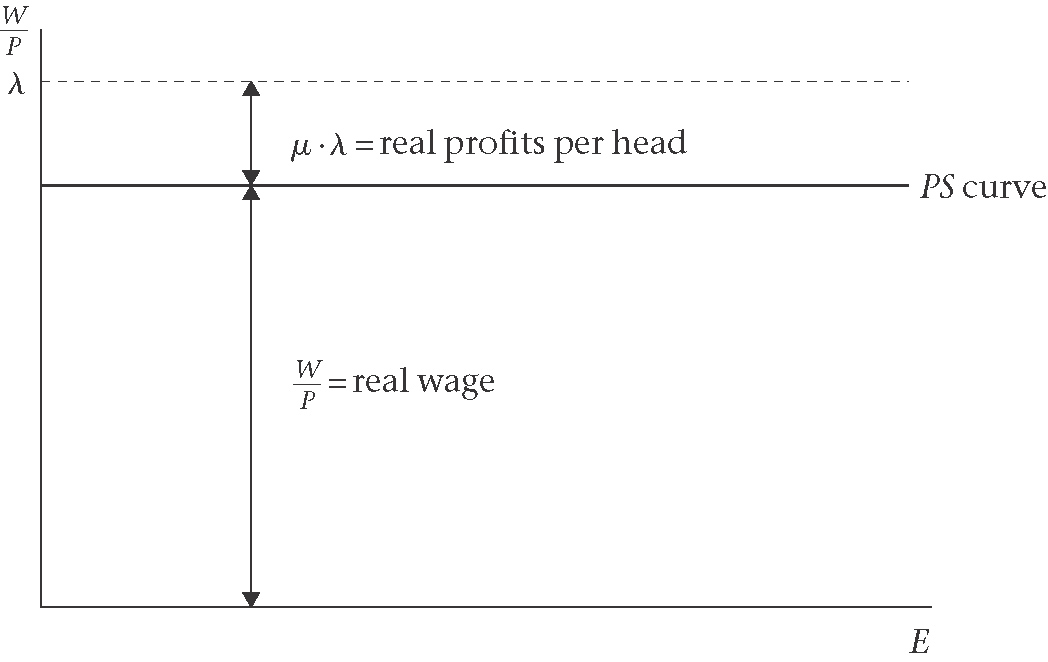
\includegraphics[width=0.7\linewidth]{Imagens/a5i13.png}
\end{figure}


\subsection{\textbf{Equilíbrio no Mercado de Trabalho}}
Equilíbrio do mercado de trabalho no médio prazo se dá pelo encontro das funções WS e PS. 

A curva de oferta de trabalho, \( WS \), cresce com o salário real. A curva \( PS \) é horizontal ou decresce com o salário real.

O equilíbrio ocorre quando as duas curvas se cruzam:

\[
b(E) = w^{WS} = w^{PS} = \lambda (1 - \mu)
\]

\[
b(E) = \lambda (1 - \mu)
\]

Define implicitamente o nível de emprego de equilíbrio de pleno emprego \( E_{ICE} \ \ ; \ \ y_e=f(E_{ICE}) \) e a taxa de desemprego \( U_{ICE} / L \) sob concorrência imperfeita.
O salário real está sempre sobre \( PS \), pois os preços são determinados logo após o salário nominal. 

Os trabalhadores estão em \( WS \) sob a suposição de que \( P = P^e \).Se \( P > P^e \), trabalhadores estarão em \( PS \) com \( E > E_{ICE} \) : ponto \( A' \).Se \( P < P^e \), trabalhadores estarão em \( PS \) com \( E < E_{ICE} \).

\subsubsection{\textbf{Qual é o timing para o ajuste de negociação de salários e preços? }}\begin{enumerate}
    \item Salário Nominal é acordado primeiro\(\rightarrow W^{WS}=P\cdot b(E)\)
    \item Dado \(W^{WS}\), empresas determinam os preços, depois do reajuste dos salários \(P^{PS}=\frac{1}{1-\mu}\cdot \frac{W^{WS}}{\mu}\), dado que há um repasse da variação nos custos ao preço final.
    \item Volume de produto e emprego são determinados pela demanda \(\rightarrow y^d\rightarrow y \rightarrow E\)
    \item Processo se repete
\end{enumerate}

Captura dois fatos estilizados: empresas são repassadoras de custos \(\rightarrow\) Desfrutam de uma vantagem comparativa 

\textbf{O que acontece quando \(y^d\)}?\begin{itemize}
    \item Inicialmente \(\pi=\pi^T \ ; \ y=y_e \ ; \ E=E_{ICE} \ ; \ \frac{\Delta W^{WS}}{W^{WS}}=\frac{\Delta P^{PS}}{W^{PS}}=\pi^T\), salário real constante.
    \item Um choque positivo de demanda\((\Delta y^d>0)\) ocasiona um crescimento no nível de produto\((y>y_e)\), o que se traduz em um desequilíbrio do mercado de trabalho, ao requerer maior volume de trabalhadores contratados\((E>E_{ICE})\). Em um primeiro momento, as empresas estão pagando o mesmo salário para um maior volume de produção. Isso gera um desequilíbrio entre o quanto as empresas estão ofertando de salários e a demanda de salários. 
    \item Assim, com maior demanda por trabalhadores, ocorre um crescimento no poder de barganha dos trabalhadores, que se traduz em um crescimento no nível de salários. Com o crescimento dos salários, após as empresas repassarem os então maiores custos aos preços, que crescem, aumenta-se a inflação\((\frac{\Delta W^{WS}}{W^{WS}}>\pi^T \ ; \ \frac{\Delta P^{PS}}{P^{PS}}>\pi^T)\). 
    \[
    \uparrow y^d \rightarrow \uparrow y \rightarrow \uparrow E =
    \]
    
    \[
    = \uparrow W^{WS} = P^e * \uparrow b(E) \rightarrow \uparrow \frac{\Delta W}{W} =
    \]
    
    \[
    = \uparrow P^{PS} = \frac{1}{1 - \mu} * \uparrow \frac{W}{\lambda} \rightarrow \uparrow \frac{\Delta P}{P}
    \]

    \begin{figure}[H]
    \centering
    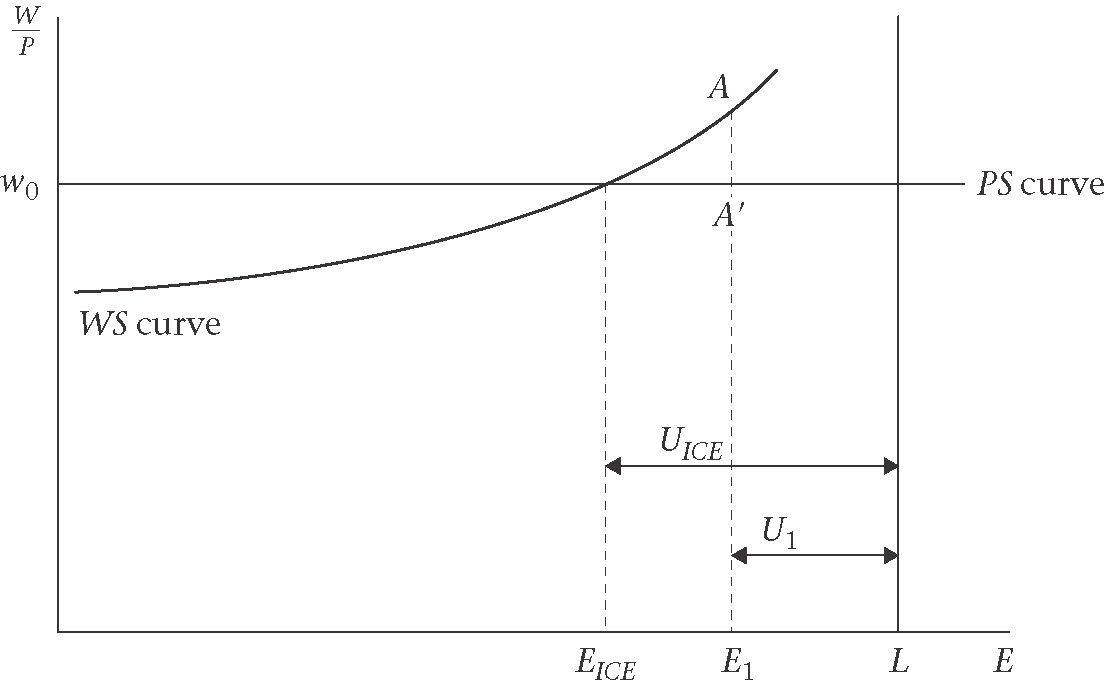
\includegraphics[width=0.7\linewidth]{Imagens/a7i1.png}
    \end{figure}

\end{itemize}

\begin{figure}[H]
    \centering
    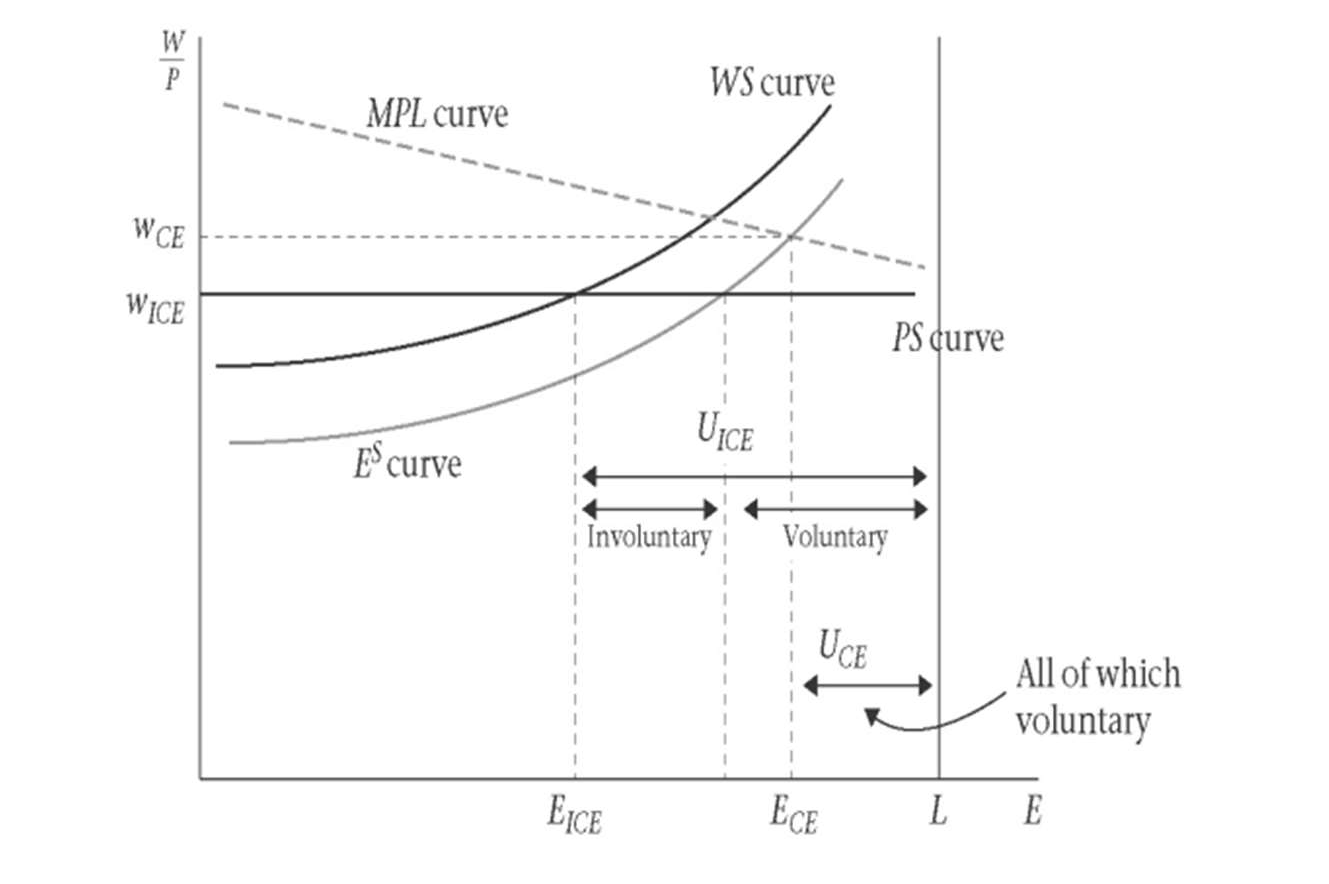
\includegraphics[width=0.7\linewidth]{Imagens/a7i2.png}
\end{figure}

Superposição das curvas \( w^{PS} \) e \( w^{WS} \), e oferta (\( E^S \)) e demanda por trabalho (\( MPL \)) permite distinguir desemprego de equilíbrio sob concorrência imperfeita e sob concorrência perfeita.

\begin{itemize}
    \item imperfeição reduz oferta de trabalho e torna \( WS > E^S \) para qualquer dado nível de emprego.
    \item imperfeição reduz oferta de produto e torna \( PS < MPL \) para qualquer dado nível de emprego.
    \item imperfeição gera desemprego involuntário.
    \item oferta de trabalho com \( w_{ICE} \) excede emprego de equilíbrio \( E_{ICE} \).
\end{itemize}

\textbf{Choques}

\begin{itemize}
    \item Menor \( b \) reduz poder de barganha dos trabalhadores, desloca \( w^{WS} \) para baixo: menor salário e maior emprego.
    \item Menor \( \mu \) reduz poder de mercado das empresas, desloca \( w^{PS} \) para cima: maior salário e maior emprego.
\end{itemize}

\newpage
\section{\textbf{Inflação, Phillips e Regras}}
\subsection{\textbf{Inflação}}
Uma medida do ritmo de crescimento dos preços. Inflação é medida como o aumento proporcional do nível de preços entre dois momentos:

\[
\pi_t = \frac{P_t - P_{t-1}}{P_{t-1}}
\]

Inflação baixa é uma conquista relativamente recente no Brasil/América Latina.

Países desenvolvidos conviveram com inflação elevada nos anos 70, mas estabilizaram suas economias nos anos 80.

Alguns custos da inflação elevada:
\begin{itemize}
    \item tende a ser volátil
    \item gera incerteza
    \item solapa a capacidade do sistema de preços de fornecer informações e guiar a alocação de recursos
    \item estabilizá-la e diminuí-la tem custos: desemprego
\end{itemize}

A  inflação  é  um  fenômeno  perene  na  história  mundial,  especialmente  na  história  latino-americana. 

\textbf{Quais são os aspectos negativos de uma inflação elevada?}\begin{itemize}
    \item Quando alta, é dificilmente regulada. Ou seja, tende a ser mais volátil quanto maior é o seu valor. Grande volatilidade pode ser traduzida como algo que gera maiores teores de incerteza  na  economia.  Em  geral,  a  incerteza  se  traduz  em  menor  eficiência  nas transações da economia, além de algo que impacta o lado microeconômico de se solapar a capacidade do sistema de preços de fornecer informações e guiar a alocação de  recursos.  As  mudanças  de  preços  como  algo  que  é  dificilmente  discernido  de mudanças dos preços relativos nos mercados é algo que também contribui para a ineficiência gerada pela inflação estar alta.
    \item É evidente, também, que existem custos para estabilizar e diminuir a inflação, sendo o principal: \textbf{a geração de desemprego}. 
\end{itemize}

\subsection{\textbf{Curva de Phillips com Inércia (PC)}}
Descreve  a  dinâmica  da  inflação  perante  os  níveis  de  produto  e desemprego. 

Inflação, segundo a Curva de Phillips, depende de: \begin{itemize}
    \item inflação corrente: \(\pi_t\)
    \item inflação passada: \(\pi_{t-1}\)
    \item hiato do produto: \(y_t-y_e\)\begin{itemize}
        \item \(y_t\): depende da demanda agregada \(y^d\)
        \item \(y_e\): depende das condições de oferta explicadas no mercado de trabalho
    \end{itemize}
\end{itemize}

\textbf{ O que justifica a inflação passada ser relevante para explicar a inflação corrente?}\begin{itemize}
    \item A dependência de \(\pi_t\) em relação a \(\pi_{t-1}\)decorre da incorporação de \textbf{INÉRCIA} ao processo inflacionário. Na física, inércia segue a ideia de uma força que continua se manifestando quando o movimento é interrompido. De forma análoga, a economia se usa desse termo para explicar que mesmo que seja aplicada uma força de sentido contrário (choques contracionistas de demanda agregada, reduzindo o emprego e o nível de atividade) à tendência de crescer a inflação, essa inflação apresentará uma resistência inercial a esses movimentos contracionistas. 
\end{itemize}

\textbf{Razões para existir inércia inflacionária:}\begin{itemize}
    \item Sob a \(WS \ ,\ W^{WS}=P^e\cdot b(E)\), é evidente que as negociações dos dissídios (acordo que acontece entre empresa e funcionários para o reajuste percentual do salário com base na inflação) ao longo de um horizonte de 1 ano, por exemplo, com salários justapostos, geram inércia no processo inflacionário. 
    \item Além disso, os mecanismos de indexação dos salários nos contratos como o trabalho, aluguel etc. também podem contribuir para a inércia da inflação. 
    \item Existe também a influência das expectativas inflacionárias como algo que se estabelece sob retrospectiva(olham para o passado, expectativas adaptativas),  ou  seja,  que  se  definem  a  partir  dos  níveis  inflacionários  já  observados, contribuindo também, consequentemente, à inércia inflacionária. 
\end{itemize}

\textbf{Mecanismos de formação de expectativas adaptativas inflacionárias com correção de erros:}
\[
\pi_t^e=\pi_{t-1}^e+a\cdot \underbrace{(\pi_{t-1}-\pi_{t-1}^e)}_\text{erro de previsão}
\]

Sendo cada uma dessas variáveis:\begin{itemize}
    \item $\pi_t^e$: inflação esperada em $t$
    \item $\pi_{t-1}^e$: inflação esperada em $t-1$
    \item $\pi_{t-1}$: inflação efetiva em $t-1$
    \item $a \to 0 \leq a \leq 1$: Intensidade da correção do erro\begin{itemize}
        \item se \(a=1\), temos uma correção integral : \(\pi_t^e=\pi_{t-1}\)
    \end{itemize}
    \item $(\pi_{t-1} - \pi_{t-1}^e)$: \textit{Erro de previsão}
\end{itemize}

Assim, com intensidade $a = 0$ $\rightarrow$ não há correção de erro, tendo-se expectativas estáticas, ou seja, não se aprende nada com o erro de previsão de um período atrás para a determinação das expectativas sobre a inflação corrente.

Com intensidade $0 < a < 1$ $\rightarrow$ há algum aprendizado com o erro de previsão sobre a inflação de um período atrás para a determinação das expectativas sobre a inflação corrente.

\[
\pi_t^e = a \cdot \pi_{t-1} + (1 - a) \cdot \pi_{t-1}^e
\]

Com intensidade $a = 1$ $\rightarrow$ Há correção integral dos erros de previsão aprendidos com a previsão realizada na inflação de um período atrás para a determinação das expectativas sobre a inflação corrente.

\[
\pi_t^e = \pi_{t-1} = \pi^I
\]

Inicialmente, vamos assumir que expectativas acerca da evolução futura dos preços não são incorporadas nas negociações salariais.

Mais à frente, incorporaremos elementos prospectivos(olham para o futuro, expectativas racionais), com expectativas acerca das realizações futuras dos preços.

Para enfatizar o papel da inércia, o componente adaptativo é denotado $\pi^I = \pi_{t-1}$, envolvendo um único período da inflação passada.

A curva de Phillips, ao incorporar ao componente de inércia, toma a forma:

\[
\pi_t = \underbrace{\pi^I}_\text{inércia inflacionária} + \alpha (y_t - y_e)
\]

Ou seja,

\[
\underbrace{\pi_t}_{\text{inflação corrente}} = 
\underbrace{\pi_{t-1}}_{\text{inflação passada}} + 
\underbrace{\alpha}_{\text{Sensibilidade da inflação ao hiato}}
\underbrace{(\underbrace{y_t}_\text{Choques de Demanda} - \underbrace{y_e}_\text{Choques de Oferta})}_{\text{hiato do produto}}
\]


Assim, \textbf{assumindo que haja 100\% de aprendizado com os erros de previsão obtidos ($\alpha = 1$)}, tem-se, portanto, que: $\pi^I = \pi_{t-1}$, tornando a PC:

\[
\pi_t = \pi_{t-1} + \alpha \cdot (y_t - y_e)
\]

\[
\Delta \pi_t = \alpha \cdot (y_t - y_e)
\]


\textbf{Exemplo:}

Suponha que $\pi_{t-1} = 4\%$, $y_{t-1} - y_e = 0$, $\alpha = 1$ e considere um choque de demanda, que eleva o emprego, produto e, portanto, a um hiato positivo de $y_t - y_e = 2\%$.

\begin{enumerate}
    \item Deduz-se que o ritmo de crescimento dos salários será: 
    \[
    \left( \frac{\Delta W}{W} \right)_t = 4\% + 2\% = \pi_t = 6\%
    \]
    
    \item Se o choque perdurar, se terá que:
    \[
    \left( \frac{\Delta W}{W} \right)_{t+1} = 6\% + 2\% = 8\%
    \]

    \item Enquanto o hiato se mantiver positivo, e o choque perdurar por $n$ períodos, os salários continuarão a elevar o seu ritmo de crescimento.
\end{enumerate}

\textbf{Observação}: Observe que embora tenhamos utilizado o hiato do produto como parâmetro para avaliar o impacto do nível de atividade à inflação, mas se poderia muito bem observar essas relações sobre outro escopo, como o exemplo da utilização do impacto dado à relação entre o nível de emprego corrente e o nível de emprego no equilíbrio no mercado competitivo imperfeito. A Lei de Okun é um exemplo de escopo diferente que se possa ser utilizado, estabelecendo uma relação empírica entre o crescimento da demanda e do produto e a redução do desemprego (ou aumento do emprego). 

Vale notar que \(\Delta \pi\)será maior, igual ou menor que 0 conforme \(y-y_e\)  é maior, igual ou menor que 0.

Observe que o deslocamento da PC ocorre quando há uma alteração do componente de inércia inflacionária. Como visto, esse componente tem a característica de criar uma resistência a mudanças inflacionárias, sendo influente para a determinação da inflação corrente. Assim, a inércia inflacionária é estruturada, dentre outras coisas, pelos ajustes salariais em relação à inflação  garantidos por contratos. O deslocamento da PC, quando ocorre um choque inflacionário derivado de uma mudança no nível de produto para além de seu nível natural, dependerá do quão longevos esses contratos são, de tal forma a se alterar para um período a frente, após serem feitos os ajustes, podendo variar entre períodos trimestrais, semestrais a anuais dependendo do país e longevidade dos contratos nessa dada economia. Por exemplo: \begin{itemize}
    \item Se a inércia em um primeiro momento for de 4\%, a inflação corrente no nível de produto de equilíbrio for 4\% e, porventura, houver um choque no nível de produto para algo além  do  nível  de  pleno  emprego.  Em  um  primeiro  momento  haverá  apenas  uma movimentação ao longo da mesma Curva de Phillips \(PC(\pi^I=4\%)\) com a variação do produto. A partir do momento que os ajustes salariais ocorrem, a PC altera o seu componente  inercial  para,  por  exemplo,  6\%,  deslocando-se  para  a  esquerda \(PC(\pi^I=6\%)\)
\end{itemize}

Uma outra maneira de pensar a Curva de Phillips seria olhando para a sua equação que inclui as expectativas inflacionárias: 
\[
\pi_t=\pi_t^E+\alpha(y_t-y_e)
\]

Sendo que há uma participação ponderada entre o quanto as expectativas são \textbf{Prospectivas} (peso à meta para a formação das expectativas) ou \textbf{Retrospectivas} (peso ao componente de inércia/inflação passada para a formação das expectativas) \(\gamma\):
\[
\pi_t=\underbrace{(1-\gamma)\cdot\pi_t^e}_\text{prospectiva}+\underbrace{\gamma\cdot\pi_{t-1}}_\text{retrospectiva}+\alpha(y_t-y_e)
\]
Com \(\gamma=1\), PC é puramente retrospectiva. Com \(\gamma = 0\), PC é  puramente prospectivas ("expectativas racionais").

É evidente, pelo comportamento da PC, a \textbf{Crítica de Lucas}. Essa crítica trazia a ideia de que um governo que tente se usar do \textit{trade-off} entre inflação e desemprego com o objetivo de manter o desemprego abaixo do ERU, eventualmente se leva a perder credibilidade no mercado e, mais para  um  médio/longo  prazo,  acaba  perdendo  eficácia  de  suas  políticas  monetárias  que objetivem  sistematicamente  regular  o  produto  para  encontrar  algum  nível  desejado  de desemprego  e  inflação.  Os  wage-setters  e  price-setters  podem  suspeitar  das  mudanças inflacionárias como sendo algo feito deliberadamente pelo governo, não alterando os seus padrões de oferta e, portanto, não alterando o nível de produto para mudanças inflacionárias. Essa crítica evidencia como, no longo prazo, sob um contexto de inflação persistentemente acelerada, se materializa uma Curva de Phillips Vertical (VPC) sob o produto potencial. 

Observe que existem alguns outros fatores que podem ocasionar essa mudança de inclinação da PC no médio/longo prazo. Dentre estas, por exemplo, seria um cenário de alta inflação. Sob esse contexto, os reajustes salariais passariam a ser mais frequentes, de forma trimestral ou bimestral,  o  que  tenderia  a  nulificar  os  efeitos  das  políticas  monetárias  que,  de  forma persistente, intencionam a acelerar a inflação. Isso porque os salários seriam ajustados já compreendendo a falta de credibilidade do Banco Central para com as suas metas inflacionárias. 

A interseção de \( PS \) com \( WS \) define equilíbrio no mercado de trabalho.

Formadores de preços e salários satisfeitos com suas remunerações e custos, sintetizados no nível do salário real de equilíbrio.

A inflação é constante no nível de desemprego de equilíbrio.

O preço é determinado por uma margem (constante) sobre o custo do trabalho por unidade do produto:

\[
P = (1 + \bar{\mu}) \times \frac{W}{\lambda}
\]

Portanto, a variação dos preços reflete a variação do custo do trabalho por unidade do produto:

\[
\frac{\Delta P}{P} = \frac{\Delta W}{W} - \frac{\Delta \lambda}{\lambda}
\]

Ou seja, a diferença entre o crescimento dos salários e da produtividade.

Se \(\lambda\) for constante, então \(\frac{\Delta \lambda}{\lambda} = 0\), logo:

\[
\frac{\Delta P}{P} = \frac{\Delta W}{W}
\]

Como desvios do nível de emprego de equilíbrio afetam a inflação?

Apesar de negociarem salários nominais, os trabalhadores se preocupam com a remuneração real esperada:

\[
W_t^{WS} = P_t^e b(E_t)
\]

A evolução dos salários nominais depende da inflação passada e do eventual desvio do emprego em relação à taxa de equilíbrio/natural.

Supondo que em \( t-1 \) a economia se encontrava em equilíbrio, com \( E = E_{ICE} \) e \( P^e = P_{t-1} \), vale a relação:

\[
W_{t-1} = P_{t-1} b(E_{ICE})
\]

Portanto, a evolução do salário nominal segue:

\[
\frac{W_t^{WS}}{W_{t-1}} = \frac{P_t^e}{P_{t-1}} \times \frac{b(E_t)}{b(E_{ICE})}
\]

Tomando logaritmos:

\[
\ln \left( \frac{W_t^{WS}}{W_{t-1}} \right) = \ln \left( \frac{P_t^e}{P_{t-1}} \right) + \ln \left( \frac{b(E_t)}{b(E_{ICE})} \right)
\]

\[
\ln \left( 1 + \frac{\Delta W_t^{WS}}{W_{t-1}} \right) = \ln \left( 1 + \frac{\Delta P_t^e}{P_{t-1}} \right) + \ln \left( \frac{b(E_t)}{b(E_{ICE})} \right)
\]

\[
\frac{\Delta W_t^{WS}}{W_{t-1}} = \pi_t^e + \ln \left( \frac{b(E_t)}{b(E_{ICE})} \right)
\]

Na presença de inércia/expectativas adaptativas, a expectativa de inflação:

\[
\pi_t^e = \pi_{t-1}
\]

Desvios do emprego em relação ao nível de equilíbrio estão relacionados a desvios do produto em relação ao nível de equilíbrio.

O poder de barganha relativo está relacionado ao hiato do produto através de:

\[
\ln \left( \frac{b(E_t)}{b(E_{ICE})} \right) = \alpha (y_t - y_e)
\]

Logo, o reajuste de salários segue:

\[
\frac{\Delta W_t^{WS}}{W_{t-1}} = \pi_{t-1} + \alpha (y_t - y_e)
\]

Se o hiato do produto (ou emprego) é não nulo:

\[
E_t \neq E_{ICE} \Rightarrow y_t \neq y_e \Rightarrow \left( \frac{\Delta W}{W} \right)_t \neq \left( \frac{\Delta P}{P} \right)_{t-1}
\]

\textbf{Cronologia dos eventos:}

Choque de demanda \(\Rightarrow\) alteração no produto e emprego \(\Rightarrow\) reajuste de salários \(\Rightarrow\) reajuste de preços imediato.

Resulta, portanto, a curva de Phillips:

\[
\pi_t = \left( \frac{\Delta P_t}{P_{t-1}} \right) = \left( \frac{\Delta W_t^{WS}}{W_{t-1}} \right) = \pi_{t-1} + \alpha (y_t - y_e)
\]

\begin{figure}[H]
    \centering
    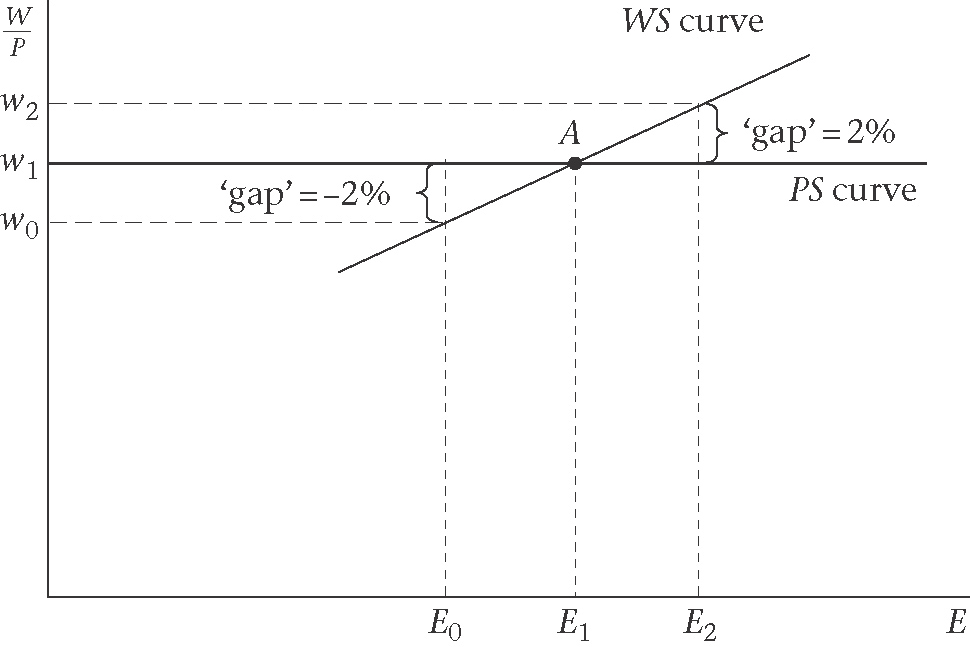
\includegraphics[width=0.7\linewidth]{Imagens/a9i1.png}
\end{figure}

\textbf{Exemplo}

Suponha que \(\pi_{t-1} = 4\%\), \(y_t - y_e = 0\), \(\alpha = 1\) e considere um choque de demanda, que eleva o emprego, o produto e, portanto, gera um hiato positivo de \(y_t - y_e = 2\%\).

\begin{enumerate}
    \item Deduz-se que o ritmo de crescimento dos salários será:
    \[
    \frac{\Delta w}{w_t} = 4\% + 2\% = \pi_t = 6\%
    \]
    
    \item Se o choque perdurar, se terá que:
    \[
    \frac{\Delta w}{w_{t+1}} = 6\% + 2\% = 8\%
    \]

    \item Enquanto o hiato se mantiver positivo, e o choque perdurar por \(n\) períodos, os salários continuarão a elevar o seu ritmo de crescimento.
\end{enumerate}

\textbf{Adendo}

Observe que, embora tenhamos utilizado o hiato do produto como parâmetro para avaliar o impacto do nível de atividade sobre a inflação, poderíamos, igualmente, analisar essas relações sob outro escopo. 

Por exemplo, poderíamos observar o impacto na relação entre o nível de emprego corrente e o nível de emprego de equilíbrio em um mercado competitivo imperfeito. 

A \textbf{Lei de Okun} é um exemplo de abordagem alternativa, estabelecendo uma relação empírica entre o crescimento da demanda e do produto e a redução do desemprego (ou aumento do emprego).

\textbf{Voltando...}

A \textbf{Curva de Phillips} é caracterizada por três parâmetros principais:

\begin{itemize}
    \item \(\pi_t - \pi_{t-1}\) define a altura da Curva de Phillips.
    \item A sensibilidade de \(\Delta \pi\) ao hiato do produto (\(\alpha\)) define a inclinação da Curva de Phillips.
    \item O produto potencial \(y_e\).
    \item Componente de inércia: \(\pi_e = \pi_{t-1}\).
\end{itemize}


\begin{table}[H]
    \centering
    \caption{Dinâmica Inflacionária}
    \begin{tabular}{|c|c|c|c|c|c|}
        \hline
        Período & Emprego & Inflação -1 & Hiato & Inflação de Salários & Inflação de Preços \\
        \hline
        0 & \(E_1\) & 4 & 0 & 4 & 4 \\
        \hline
        \multicolumn{6}{c}{\textbf{Inflação constante}} \\
        \hline
        1 & \(E_1\) & 4 & 0 & 4 & 4 \\
        2 & \(E_1\) & 4 & 0 & 4 & 4 \\
        3 & \(E_1\) & 4 & 0 & 4 & 4 \\
        \hline
        \multicolumn{6}{c}{\textbf{Inflação crescente}} \\
        \hline
        1 & \(E_2\) & 4 & 2 & 6 & 6 \\
        2 & \(E_2\) & 6 & 2 & 8 & 8 \\
        3 & \(E_2\) & 8 & 2 & 10 & 10 \\
        \hline
        \multicolumn{6}{c}{\textbf{Inflação declinante}} \\
        \hline
        1 & \(E_0\) & 4 & -2 & 2 & 2 \\
        2 & \(E_0\) & 2 & -2 & 0 & 0 \\
        3 & \(E_0\) & 0 & -2 & -2 & -2 \\
        \hline
    \end{tabular}
\end{table}

Equilíbrio no mercado de trabalho e a curva de Phillips: relacionada a \( WS \) e \( PS \).

\textbf{Lei de Okun}: relação empírica entre crescimento da demanda e do produto e redução do desemprego ou (aumento do emprego).

Permite associar o nível de emprego no gráfico superior ao nível de produto no gráfico inferior.

\( E \) (ou desemprego) e \( y \) não guardam uma relação de proporcionalidade estritamente unitária.

É possível observar \( \Delta y > 0 \) com \( \Delta E = 0 \) na saída de uma recessão \(\rightarrow\) retenção de trabalhadores sem demissão pode ser eficiente.

É possível observar \( \Delta y > 0 \), \( \Delta E > 0 \) e \( \Delta U = 0 \) na saída de uma recessão \(\rightarrow\) maior participação na força de trabalho em momentos de expansão econômica.


\begin{figure}[H]
    \centering
    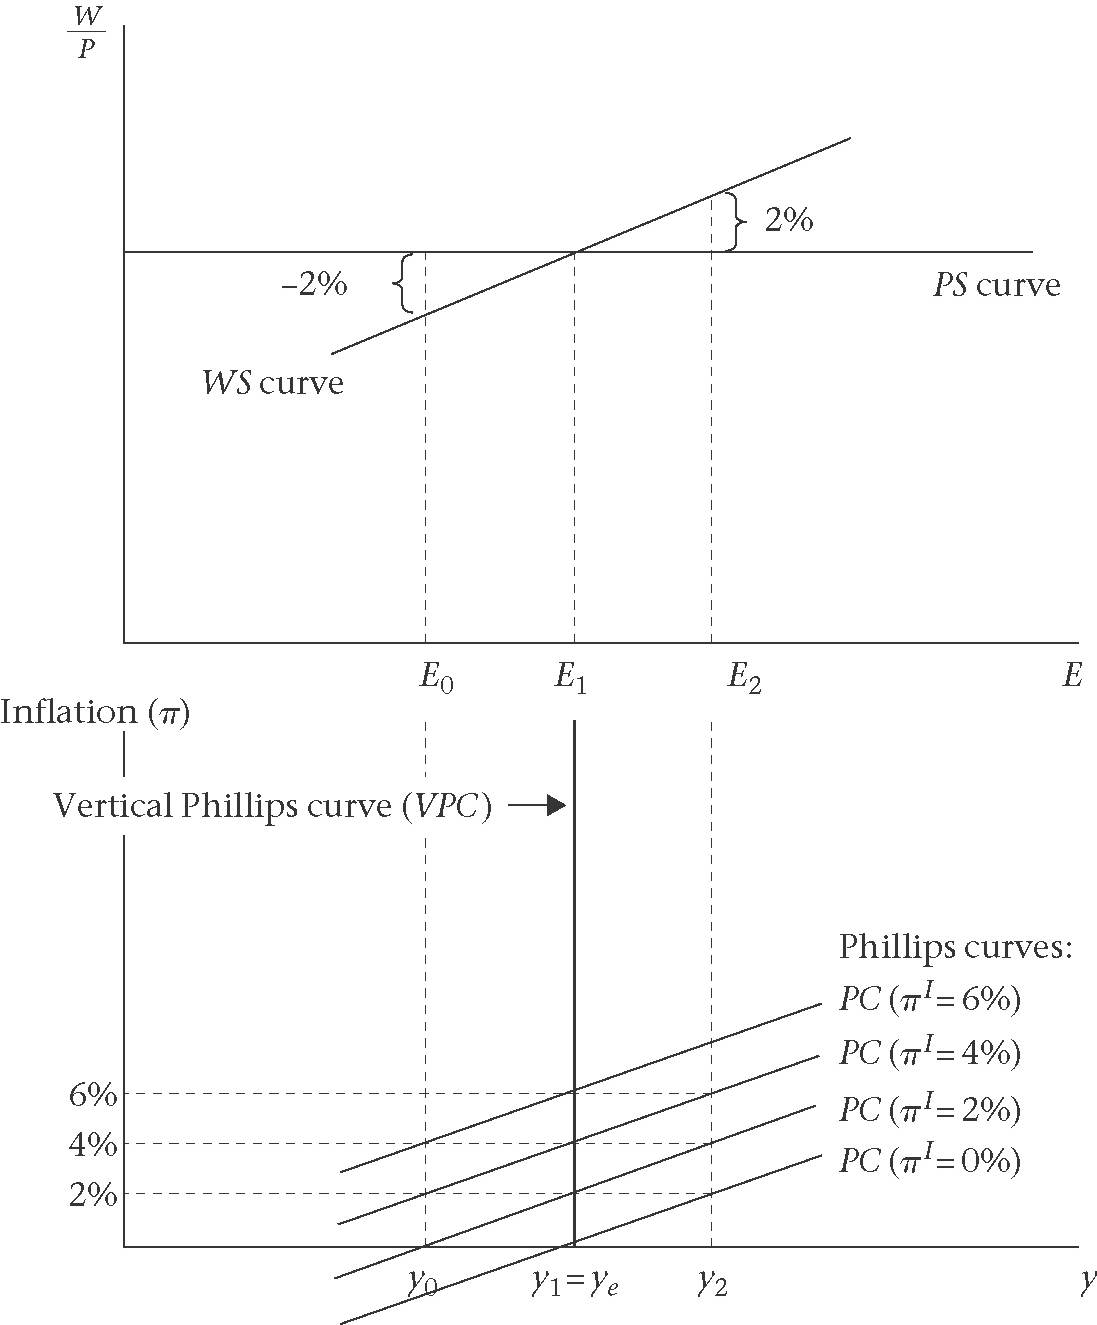
\includegraphics[width=0.7\linewidth]{Imagens/a9i2.png}
\end{figure}

A curva de Phillips é sintetizada por duas características:

\begin{itemize}
    \item \textbf{Inflação defasada} \(\Rightarrow\) estabelece a altura da curva de Phillips quando o desemprego está no nível de equilíbrio.
    \item  Capta o nível de produto e inflação consistentes com estabilidade inflacionária.
    \item \textbf{Inclinação da função \(WS\)} \(\Rightarrow\) estabelece a inclinação da curva de Phillips.
    \item Capta a relação entre desvios do nível de emprego (ou produto) em relação ao valor de equilíbrio e variações da taxa de inflação.
    \item Onde a inclinação da PC é definida pelo \(\alpha\) e a altura é definida por \(\pi_{t-1}\ \  \text{e}\ \ y_e \)
\end{itemize}

\[
\pi_t = \pi_{t-1} + \underbrace{\alpha}_\text{inclinação da PC} (y_t - y_e)
\]

\[
\underbrace{\pi_t}_{\text{inflação corrente}} = \underbrace{\pi_{t-1}}_{\text{inflação passada}} + \underbrace{\alpha (y_t - y_e)}_{\text{hiato do produto}}
\]

\textbf{Versão aceleracionista:}

\[
\alpha (y_t - y_e) \begin{cases} 
> 0 \\ 
= 0 \\ 
< 0 
\end{cases} 
\Rightarrow \Delta \pi_t 
\begin{cases} 
> 0 \\ 
= 0 \\ 
< 0 
\end{cases}
\]

A curva de Phillips se desloca quando o valor da inflação defasada muda.

A política macroeconômica é capaz de deslocar a economia de \( A \to B \)? \begin{itemize}
    \item Atingir um menor nível de desemprego às custas de uma inflação um pouco mais alta?
\end{itemize}

\begin{figure}[H]
    \centering
    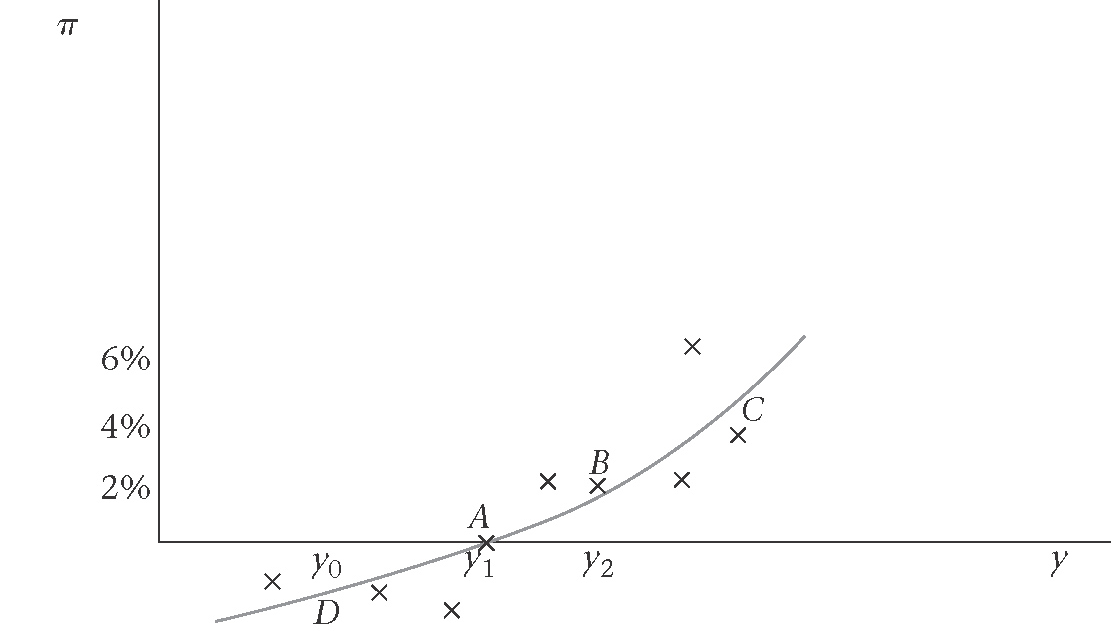
\includegraphics[width=0.7\linewidth]{Imagens/a9i3.png}
\end{figure}


A perspectiva de manter o nível de produto em \( B \) de maneira duradoura em algum momento forçará um ajuste nos salários, nos preços e nas expectativas inflacionárias. \begin{itemize}
    \item A curva de Phillips se desloca para cima: \textbf{trade-off} entre \( \pi \) e \( y \) é enfraquecido.
    \item A busca de \( B \) de maneira sistemática acabará gerando uma taxa de inflação crescente.
    \item Inicialmente, o ajuste das expectativas decorre da simples correção do erro passado.
    \item Erros persistentes geram aprendizado: o próprio processo de formação de expectativas evolui.
    \item Regras de projeção da inflação mais racionais, que evitem erros sistemáticos, eliminam ganhos no produto.
\end{itemize}

\( CP \) vertical no longo prazo ou quanto mais veloz o ajuste de expectativas, preços e salários. \begin{itemize}
    \item Incorpora a crítica de Lucas: governos que tentem explorar de maneira sistemática o *trade-off* "darão com os burros n'água".
    \item \( CP \) só é estável se a política monetária mirar na taxa de desemprego de equilíbrio.
    \item Política anticíclica só será eficaz se não descambar para um ativismo monetário excessivo.
    \item Ancoragem das expectativas é crucial para a eficácia da política monetária.
\end{itemize}

\subsection{\textbf{Desinflação}}

Desinflação é custosa: requer uma elevação transitória da taxa de desemprego.

Redução na demanda cria folga no mercado de trabalho.

Menor poder de barganha modera o crescimento dos salários nominais e preços.

Partindo de um cenário em que \(\pi_t>\pi^T\).\textbf{Objetivo}:  Atingir  o  equilíbrio  interno:  (inflação  convergindo  à  meta  e  produto convergindo ao potencial). 


\[
E < E_{ICE}
\]
gera um hiato negativo entre as curvas \( WS \) e \( PS \).

\[
\pi_t = \pi_{t-1} + \alpha (y_t - y_e) \Rightarrow \Delta \pi_t = \alpha (y_t - y_e)
\]

\[
\Delta \pi_t < 0 \implies \alpha (y_t - y_e) < 0
\]

\[
\implies y_t < y_e
\]

A economia está em \( B \), a inflação inicial é \( 8\% \) e a meta é \( 2\% \) no ponto \( A \).

A inércia ou resistência inflacionária torna a desinflação custosa.

Impõe-se \( y_t < y_e \) ao longo da trajetória de desinflação: 

\[
B \to F \to F'
\]

A curva de Phillips (\( PC \)) se desloca sucessivamente para baixo, até atingir o novo equilíbrio.

Sem inércia, com convergência das expectativas, seria potencialmente possível uma desinflação \( B \to A \) sem custos, com \( y_t = y_e \) ao longo da transição.

\begin{figure}[H]
    \centering
    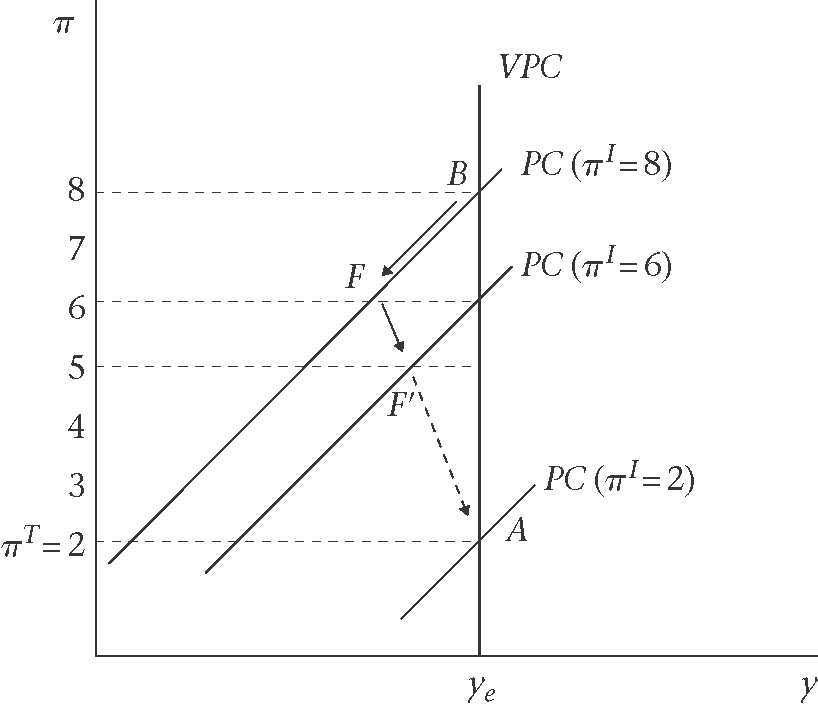
\includegraphics[width=0.7\linewidth]{Imagens/a10i1.png}
\end{figure}

\begin{figure}[H]
    \centering
    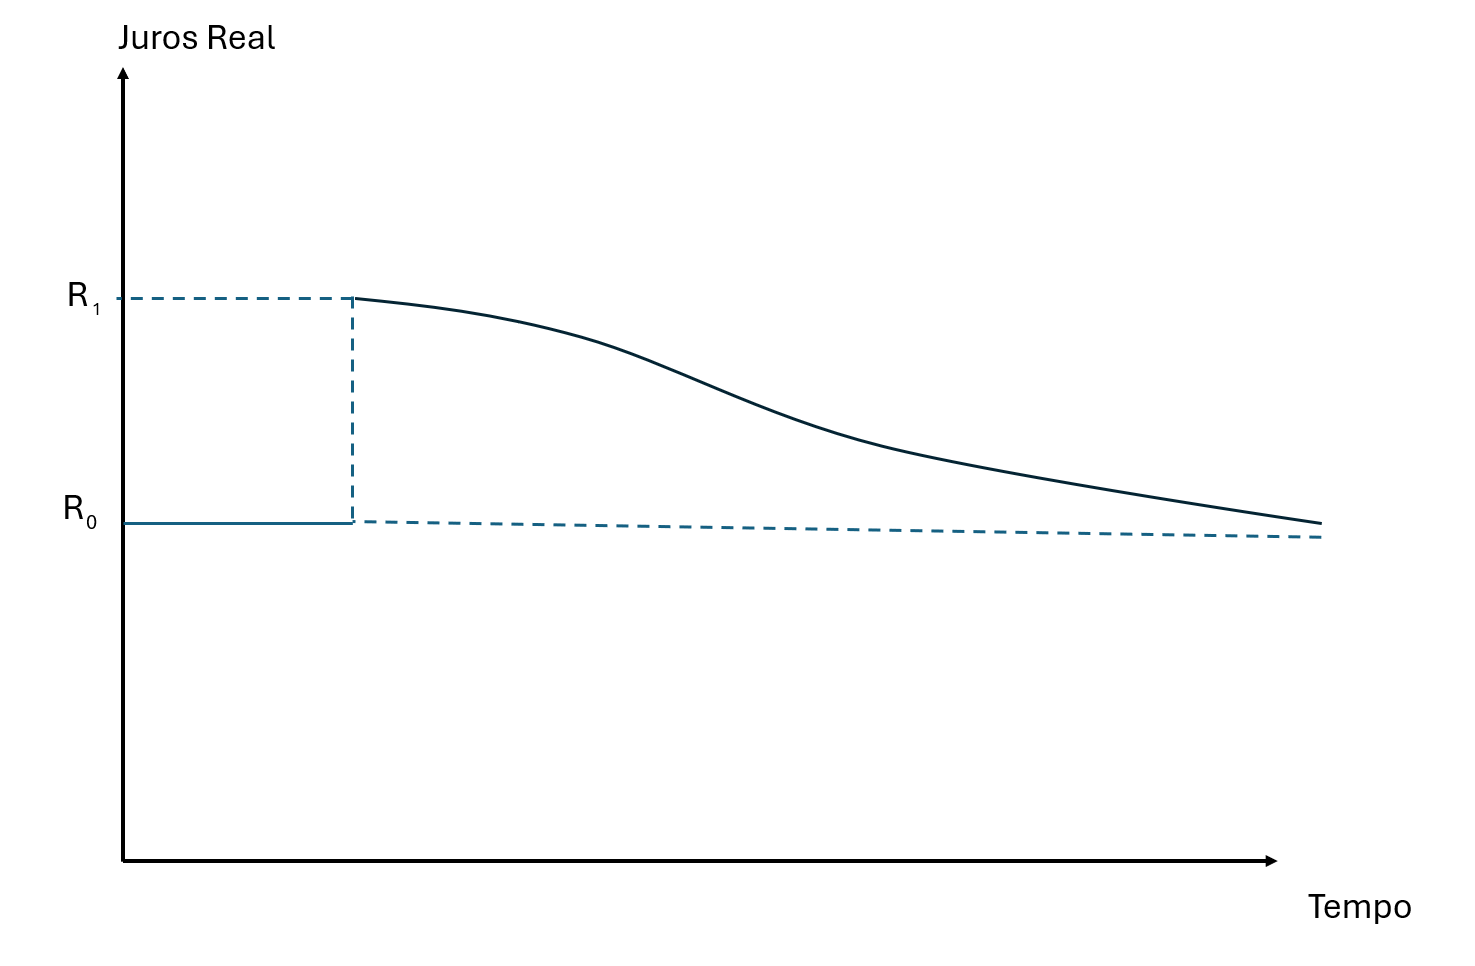
\includegraphics[width=0.7\linewidth]{Imagens/a10i2.png}
\end{figure}

\begin{figure}[H]
    \centering
    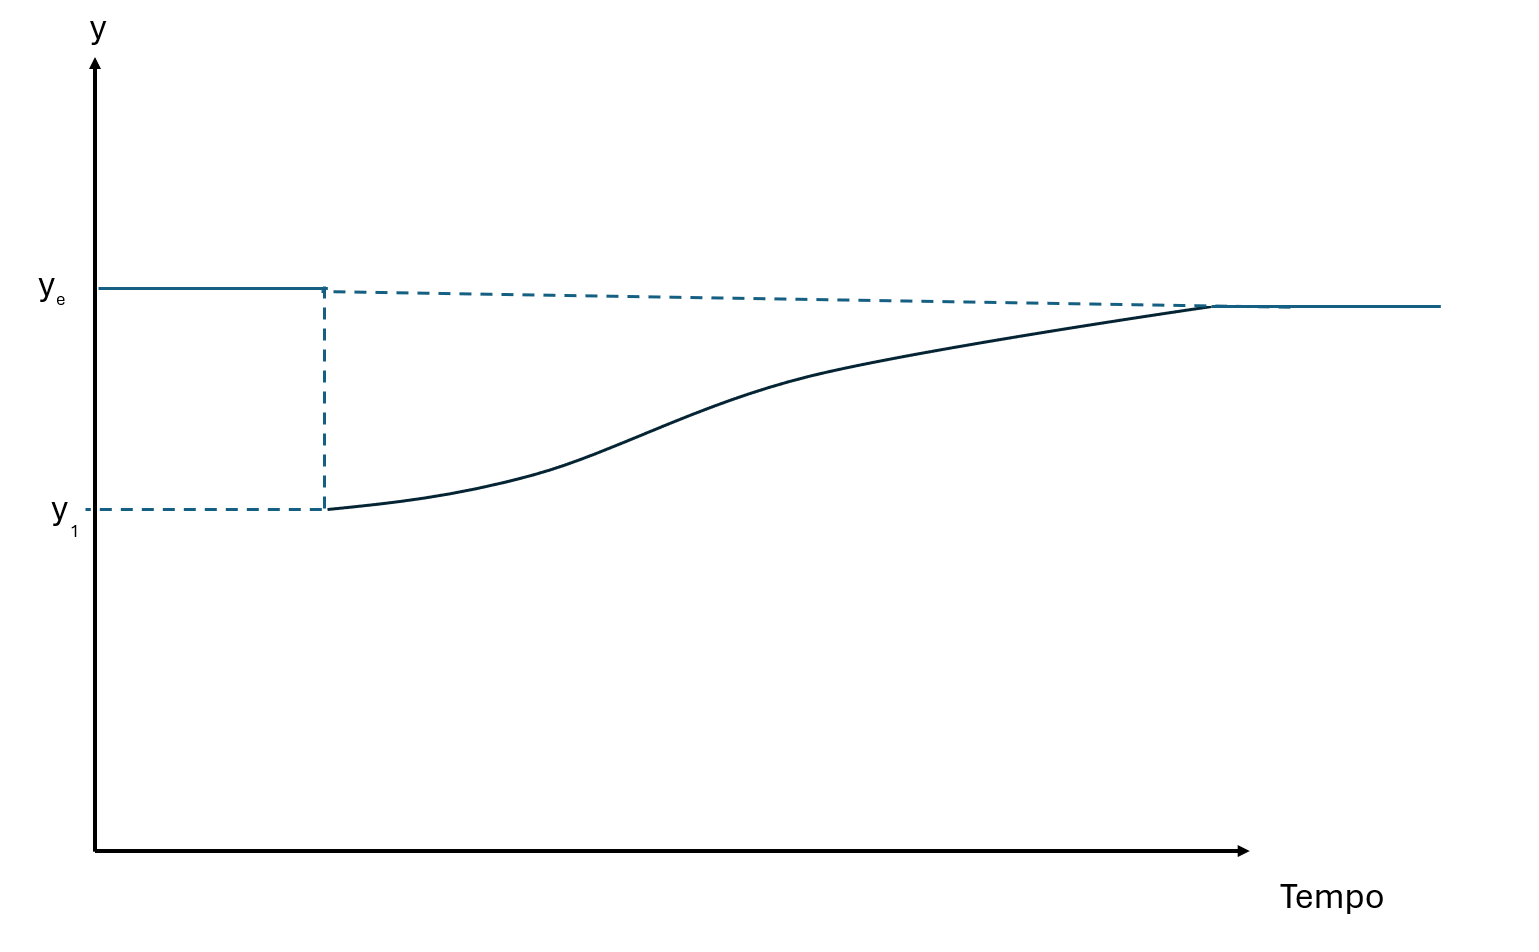
\includegraphics[width=0.7\linewidth]{Imagens/a10i3.png}
\end{figure}

\begin{figure}[H]
    \centering
    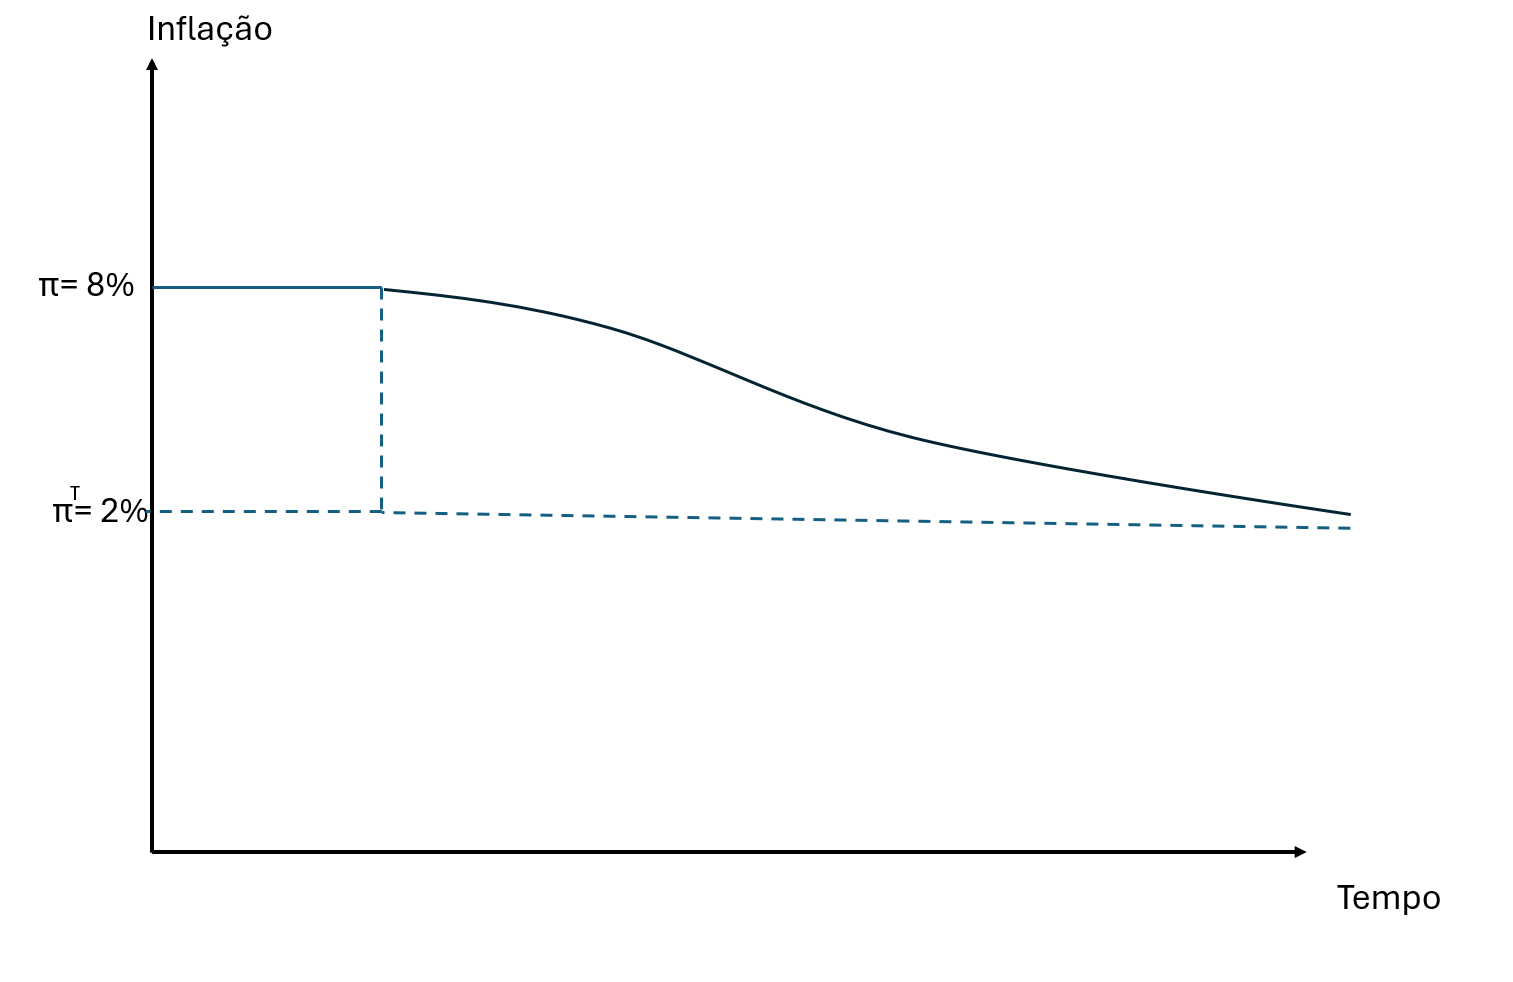
\includegraphics[width=0.7\linewidth]{Imagens/a10i4.png}
\end{figure}

Para realizar uma desinflação, indo de \( B \) para \( A \), a não ser que se tenha um ambiente sem a existência de inércia inflacionária e que todos os participantes do mercado acreditem que a meta convergirá à meta, não é possível ir diretamente. Isso, pois existe um custo em termos de desemprego para reduções da inflação. Assim, para que se reduza a inflação, é necessário que se reduza o nível de produto e emprego, elevando a taxa de desemprego para além do ERU momentaneamente. Os gráficos acima expressam como essa desinflação ocorre ao longo do tempo para o nível de produto, taxa de juros e o nível inflacionário.

\[
\Delta E < 0 \ \text{ou}\ \Uparrow U \rightarrow b(\downarrow E) 
\Rightarrow \frac{\Delta W}{W} < 8\% \Rightarrow \Delta \pi < 0 
\]
\[
\rightarrow \downarrow i \rightarrow \downarrow r \rightarrow \downarrow y^d 
\rightarrow \downarrow y \rightarrow \downarrow E \rightarrow \Delta E \ll 0 \rightarrow \ldots
\]


Observa-se a maneira pela qual, dependendo das preferências do Banco Central perante seu teor de aversão à inflação e aversão ao desemprego, ele poderá optar por diferentes tipos de políticas para a Curva de Phillips. Se o Banco Central apresentar uma aversão maior à inflação, ele optará por mudanças no mercado de bens e serviços que garantam uma desinflação rápida, independente do custo em desemprego que se geraria. Assim, o caminho \( B \rightarrow C \rightarrow A \) no gráfico acima expressa bem esse tipo de preferência do Banco Central, sendo evidente que esse grande choque de produto abaixo do potencial ocasionaria uma grande elevação no nível de desemprego.


\subsection{\textbf{O papel do Banco Central}}
Lembrando que o Banco Central busca atingir o equilíbrio interno: \begin{enumerate}
    \item \(\pi_t\rightarrow \pi^T\): Meta inflacionária
    \item \(y_t\rightarrow y_e\): Produto Natural, de pleno emprego 
    \item \(E\rightarrow E_{ICE}\): Equilíbrio de Médio Prazo
\end{enumerate}

Várias trajetórias alternativas de desinflação são possíveis e factíveis, mas: qual será escolhida? Por quê? Com que critérios?

Uma possibilidade extrema é \( C \) - \textit{cold turkey} ou choque:

\begin{itemize}
    \item Atinge o alvo (potencialmente) em um período.
    \item Ao custo de um aumento considerável do desemprego.
    \item Combinação de resistência inflacionária com surpresa desinflacionária causa desemprego excessivo.
    \item Ajuste das expectativas gera o deslocamento \( PC(\pi^I = 8\%) \rightarrow PC(\pi^I = 2\%) \).
    \item A política monetária pode então ser relaxada e \( C \rightarrow A \) com \( y \rightarrow y_e \).
\end{itemize}

\begin{figure}[H]
    \centering
    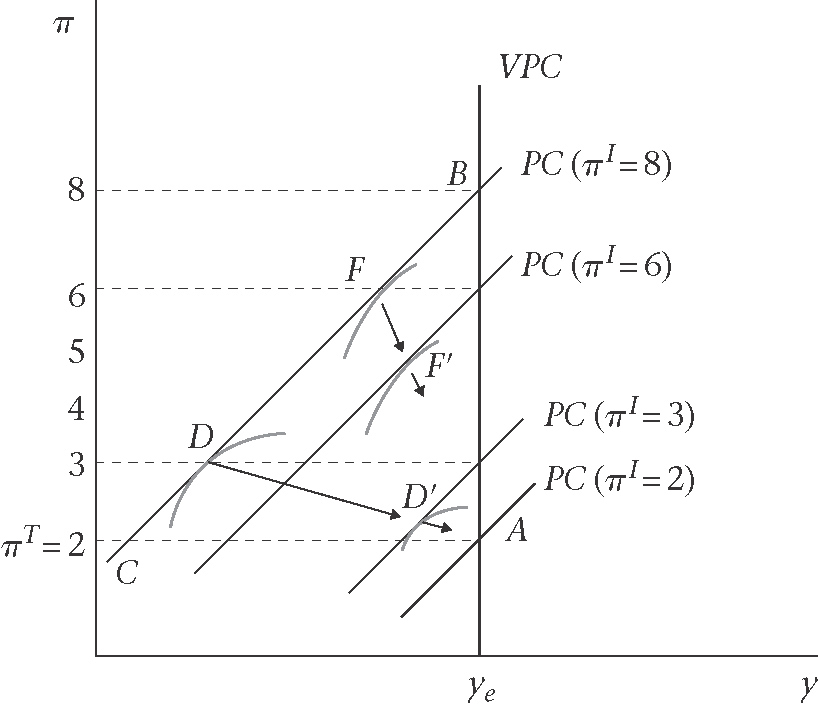
\includegraphics[width=0.7\linewidth]{Imagens/a10i5.png}
\end{figure}

Trajetórias alternativas de desinflação:\begin{enumerate}
    \item \(B\rightarrow F \rightarrow F'\rightarrow ....\rightarrow A\): Reflete a ação de um Banco Central relativamente tolerante com a inflação e intolerante com desvios do pleno emprego. "Dovish" e Pombini.
    \item \(B\rightarrow D \rightarrow D'\rightarrow ....\rightarrow A\): Reflete a ação de um Banco Central relativamente intolerante com a inflação e relativamente tolerante com desvios do pleno emprego. "Hawkish" e Gavionini.
    \item \(B\rightarrow F \rightarrow F'\rightarrow ....\rightarrow A\): Reflete a ação de um Banco Central  intolerante com a inflação e totalmente tolerante com desvios do pleno emprego. Chamado de \textbf{"Cold Turkey"}.
\end{enumerate}

A Regra Monetária (MR) é a função de reação do Banco Central aos desequilíbrios de inflação e produto. Essa função guia as ações do Banco Central na busca de seus objetivos levando em conta as suas preferências. Objetivos do Banco Central seriam, portanto, convergir o nível inflacionário à meta e convergir o nível de produto ao pleno emprego.

É evidente por essa função o perfil do Banco Central quanto às suas aversões à inflação e ao desemprego, ou seja, se esse agente está tomando preferência mais agressivas ou conservadoras quanto ao nível de atividade econômica (hawkish ou dovish).

É então evidente, pela \textbf{Regra Monetária}, as combinações de inflação e produto (\(\pi, y\)) que são coerentes com as preferências do Banco Central, as combinações que seriam \textbf{DESEJÁVEIS}. Já a \textbf{Curva de Phillips} traça aquelas combinações de inflação e produto que são \textbf{FACTÍVEIS}.

Assim, o Banco Central irá ponderar pela Regra Monetária entre os desvios no nível de atividade (observando o hiato do produto) e os desvios no nível de inflação (observando a diferença entre a inflação corrente e a meta; A compatibilização dos pares \((\pi \ , \ y)\) factíveis + desejáveis = Escolha ótima). A Equação irá expressar o quão sensível o Banco Central está a variações inflacionárias ao custo dos desvios no produto. Essa sensibilidade (\textit{``b''}) é então um coeficiente que depende das preferências do Banco Central e da Curva De Phillips (factibilidade dessas preferências).

\subsection{\textbf{Demanda Agregada e IS}}
De forma a simplificar a curva IS, apresenta-se:
\[
y = y^d = A - a * r \tag{1}
\]

Sendo que, ``\( A \)'' aqui deixa de ser apenas os ``Animal Spirits'', ou componente autônomo associado ao nível de investimento, passando a abranger \textbf{TODOS} os componentes exógenos/autônomos da demanda.

\textbf{Assim, nesse contexto, lembra-se que o produto de pleno emprego se define por:}

\[
y_e = f(E_{ICE})
\]

Trabalhar com a IS tendo como referência o produto no nível de pleno emprego significa que se destacará apenas um ponto da curva, que será aquele que apresenta o produto no nível de pleno emprego. Dessa forma, nesse selecionado ponto, tem-se uma taxa de juros que estabiliza a demanda no nível de produto de pleno emprego. Essa taxa será nomeada ``\( r_s \)''.

\textbf{Fica:}

\[
y_e = A - a * r_s \tag{2}
\]

\( r_s \rightarrow\)  Taxa que estabiliza a demanda no nível de pleno emprego, podendo ser chamada de taxa real de juros NEUTRA. Esse nome deriva da ideia de ser uma taxa de juros que neutraliza os desequilíbrios entre demanda e oferta de bens, convergindo o produto ao seu nível potencial.

\textbf{Fazendo a subtração entre (1) e (2), entende-se a seguinte interpretação alternativa da IS:}

\[
y - y_e = A - A - a * (r - r_s)
\]

\textbf{Equação alternativa da IS:} 

\[
{y - y_e = -a * (r - r_s)}
\]

Essa equação nos permite, portanto, identificar o impacto que os distanciamentos entre a taxa efetiva de juros e a taxa neutra de juros garantem em distanciamento entre o produto corrente e o potencial(do lado esquerdo é o hiato; sem defasagens). 

\subsection{\textbf{Curva de Phillips}}
Sem defasagens:
\[
\pi_t = \pi^I + \alpha (y_t - y_e)
\]


\subsection{\textbf{Regra Monetária (MR)}}



\[
y - y_e = -b * (\pi - \pi^T)
\]

Definido o par \((\pi, y)\) desejável e factível (ou seja, que satisfaz as preferências do Banco Central e é possível de ser alcançado segundo a Curva de Phillips), o Banco Central implementa a política necessária para atingi-lo.

O instrumento de política do Banco Central para a transmissão de seu alvo proposto é a taxa nominal de juros (\textit{i}):

\[
i \to r \to \text{(pela IS)} \to y^d \to y \to E \to b(E) \to \frac{\Delta W}{W} \to \frac{\Delta P}{P} = \pi
\]

A regra monetária depende das preferências do Banco Central e da sociedade, que dão forma à tolerância relativa entre desvios da inflação e do emprego em relação aos níveis almejados.

A regra monetária é uma função de reação do BC, resultante das preferências associadas ao trade-off entre inflação e desemprego.

Mais sobre isso mais à frente.

Regra monetária, obtida a partir da maximização da função objetivo do BC, cuja CPO é:

\[
y_t - y_e = -b \left( \pi_t - \pi^T \right) \rightarrow \pi_t= \pi^T-\frac{1}{b}(y_t-y_e)
\]

Combinação ótima \((y, \pi)\) que o BC escolhe, dada a Curva de Phillips, em função de suas preferências.

Se a inflação é elevada, \(\pi_t > \pi^T\), o BC aumentará a taxa de juros, reduzindo demanda, \(y_t < y_e\), para reduzir a inflação.

\(b\) reflete o custo de oportunidade de desequilíbrios inflacionários vs. desequilíbrios no produto. Reflete a interação entre as preferências do BC e das condições estruturais da economia (PC).

Maior \(b\) significa maior aversão inflacionária do BC: topa um maior sacrifício do produto/emprego, isso resulta em, caso ele vá para o infinito,c "\textit{Cold-Turkey}". Se o \(b=0\), temos um BC que não liga para os desvios inflacionários(completa acomodação), dado que sua preocupação pelo produto no pleno emprego.


\begin{figure}[H]
    \centering
    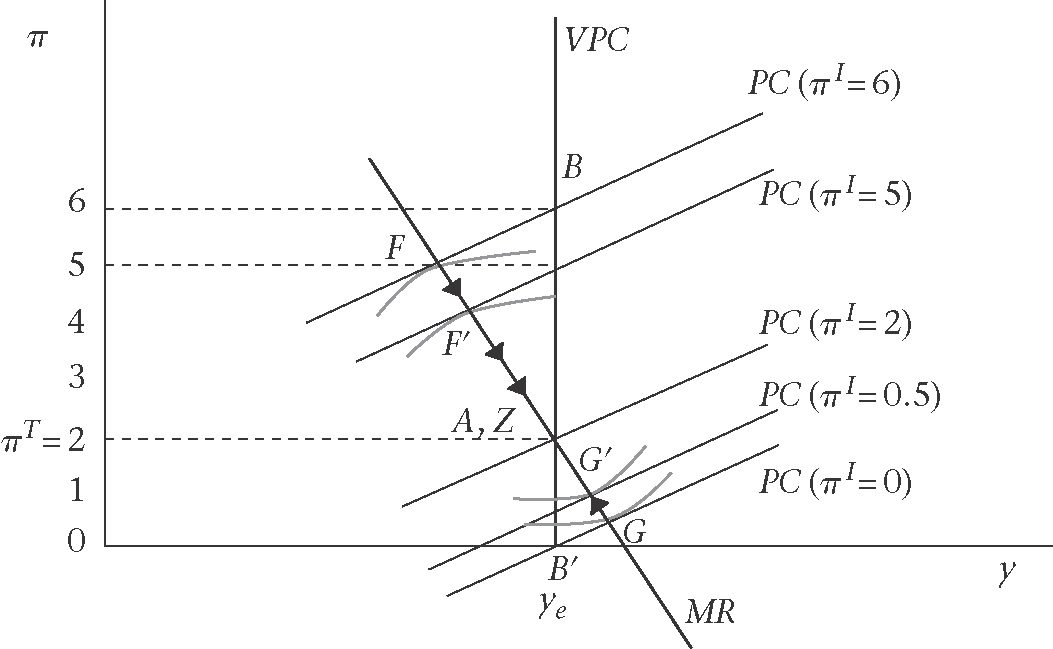
\includegraphics[width=0.7\linewidth]{Imagens/a12i1.png}
\end{figure}

A regra monetária estabelece a trajetória da economia em função das ações do BC: \begin{itemize}
    \item ao buscar restabelecer o produto de equilíbrio e a inflação condizente com a meta inflacionária;
    \item ao identificar a melhor resposta de política dada a Curva de Phillips com que se depara;
    \item ao equalizar o custo marginal do hiato do produto (em relação ao equilíbrio) ao benefício marginal da aproximação da meta inflacionária.
\end{itemize}

O instrumento de política monetária é a taxa nominal de juros.

A variável intermediária que o BC busca atingir é a taxa real de juros.

BC exerce controle indireto sobre ela, dadas as expectativas inflacionárias.

Através da taxa real de juros, o BC busca influenciar a demanda agregada.

A evolução da demanda agregada baliza o comportamento do produto e da inflação.

\subsection{\textbf{Choques Inflacionários}}
Considerando uma economia inicialmente em equilíbrio interno (inflação na meta e produto no pleno emprego). Nesse contexto, imagine que ocorra um \textbf{choque inflacionário positivo} (por conta,  por  exemplo,  de  mudança  em  expectativas)  que  desloque  a  Curva  de  Phillips verticalmente, mantendo produto sob o nível de pleno emprego. 

Situação inicial da economia \begin{itemize}
    \item economia começa em equilíbrio A com \(y=y_e \ , \ \pi=\pi^T=2\%\)
    \item choque desloca a economia para B , com a inflação de \(\pi = 4\%\)
\end{itemize}

\begin{figure}[H]
    \centering
    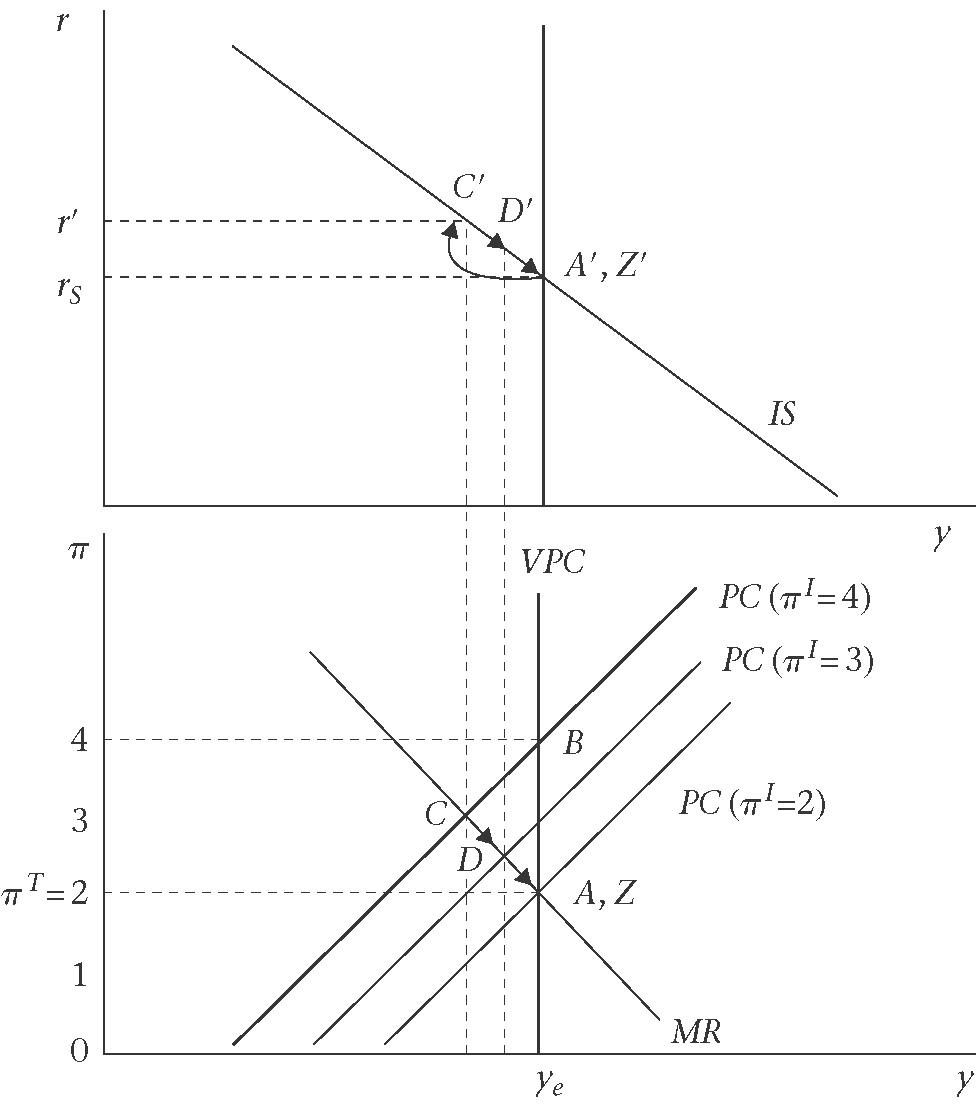
\includegraphics[width=0.7\linewidth]{Imagens/a13i1.png}
\end{figure}

\begin{figure}[H]
    \centering
    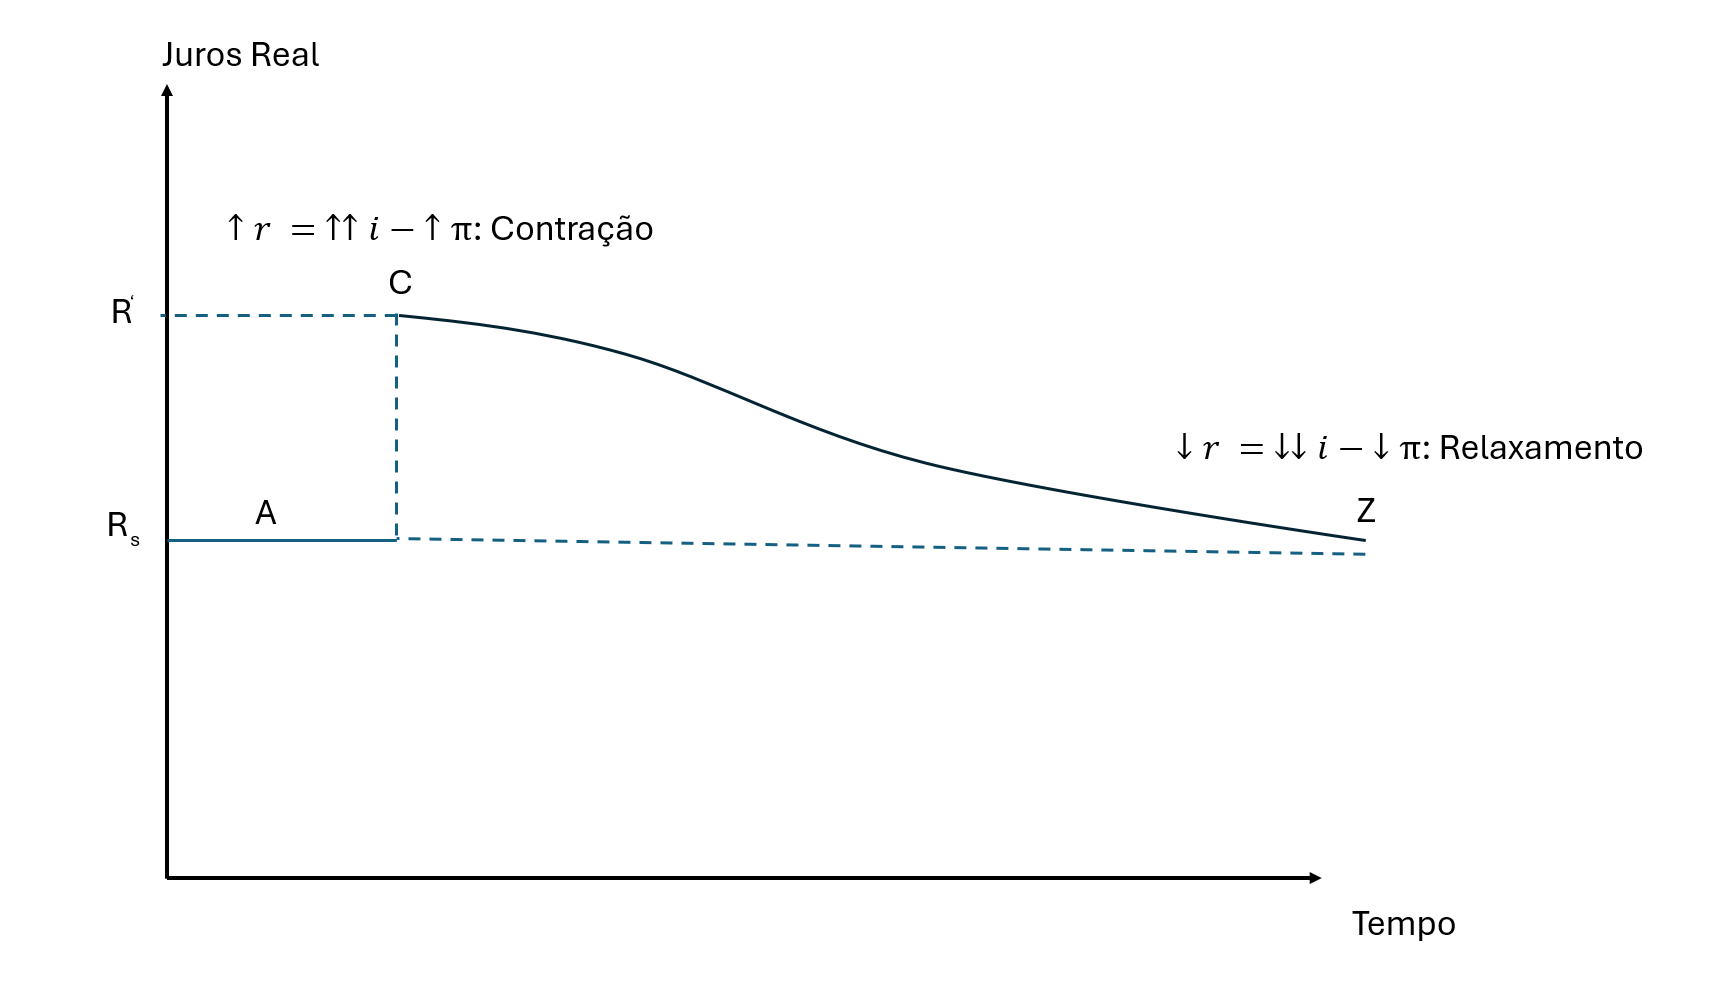
\includegraphics[width=0.7\linewidth]{Imagens/a13i4.png}
\end{figure}

Sob esses 2\% de variação na inflação, se o Banco Central elevasse a taxa nominal de juros em apenas 2\%, não haveria variação na taxa real de juros, mantendo a inflação constante sobre o nível de 4\%. Assim, para convergir a inflação à meta de 2\%, o Banco Central precisaria aumentar a taxa de juros em, pelo menos algo acima de 2\% de incremento. Ao longo da trajetória de desinflação, o hiato se manterá negativo, diminuindo em valor absoluto (aproximando produto efetivo do potencial). (A\(\rightarrow\)CHOQUE INFLACIONÁRIO\(\rightarrow B \rightarrow C \rightarrow D \rightarrow Z\) 

em resposta BC eleva a taxa de juros para \( r' > r \), contraindo a demanda agregada

nova configuração é \( C' \), \( C \) com \( y < y_e \) e \( \pi < 4\% \)

\begin{itemize}
    \item componente de inércia é revisado: \( \pi^I = 3\%\); mas como \( y < y_e \), \( \pi < 3\% \)
    \item com \( \pi < 3\% \) há algum relaxamento monetário, a taxa de juros diminui: \( C' \to D' \) e \( C \to D \)
    \item revisão continuada de \( \pi^I \) até atingir \( 2\% \) e \( r \to r_s \) com \( y \to y_e \) no ponto \( Z \)
    \item ajustes na taxa de juros seguem a regra monetária
\end{itemize}

\subsection{\textbf{Choque de Demanda: Temporário}}

\(\Rightarrow \uparrow y^d \Rightarrow \uparrow y \Rightarrow E \Rightarrow \uparrow \frac{\Delta W}{W} \Rightarrow \uparrow \pi \)

Inicialmente (A): \( y = y_e \); \( \pi = \pi^T \); \( r = r_s \)

A economia começa em equilíbrio \( A, A' \) com \( y = y_e \), \( r = r_s \) e \( \pi = \pi^T = 2\% \).

\begin{figure}[H]
    \centering
    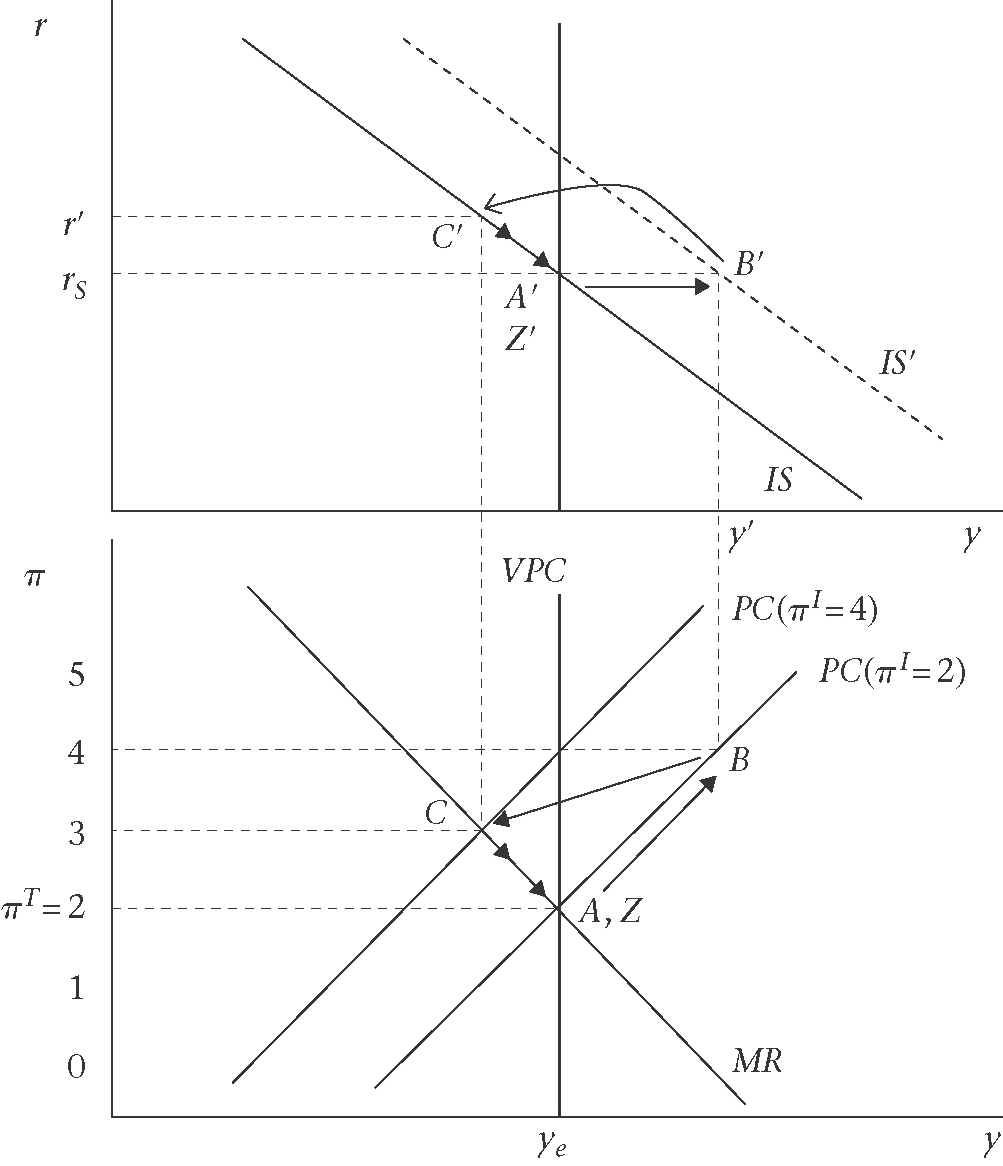
\includegraphics[width=0.7\linewidth]{Imagens/a13i2.png}
\end{figure}

Se o Banco Central não fizer nada, mesmo que o produto retorne ao pleno emprego conforme os preços sobem no longo prazo, por conta da inércia inflacionária, o equilíbrio se encontrará sob um nível inflacionário mais alto. Assim, se desejado manter o nível de inflação na meta, ele precisará movimentar a taxa de juros para combater esse efeito secundário do choque de demanda sobre o nível de inflação. Da mesma maneira que o exemplo do choque de inflação, o Banco Central irá inflar a taxa de juros de tal forma a elevar a taxa real de juros, criando um hiato do produto negativo e eventualmente encontrando o equilíbrio interno inicialmente observado.

\noindent (A \( \Rightarrow \) CHOQUE DE DEMANDA TEMPORÁRIO \( \Rightarrow \) B \( \Rightarrow \) C \( \Rightarrow \) Z)

O choque desloca \( IS \to IS' \) por um período, fazendo \( y > y_e \) e levando a inflação \( \pi = 4\% > \pi^T = 2\% \) nos pontos \( B \) e \( B' \).

O choque de demanda corrente alimenta a inflação base no período seguinte: \( \pi^I = 4\% \), deslocando \( PC \).

A melhor resposta do BC é uma elevação da taxa de juros: \( r' > r_s \) com \( y < y_e \) com \( 2\% < \pi < 4\% \).

A economia transita nos pontos \( B \to C \) e \( B' \to C' \) até convergir para \( Z, Z' \).

\subsection{\textbf{Choque de Demanda: Permanente}}

A economia começa em equilíbrio \( A, A' \) com \( y = y_e \), \( r = r_s \) e \( \pi = \pi^T = 2\% \).

O choque desloca \( IS \to IS' \) permanentemente, fazendo \( y > y_e \) e levando a inflação \( \pi = 4\% > \pi^T = 2\% \) nos pontos \( B \) e \( B' \).

\begin{figure}[H]
    \centering
    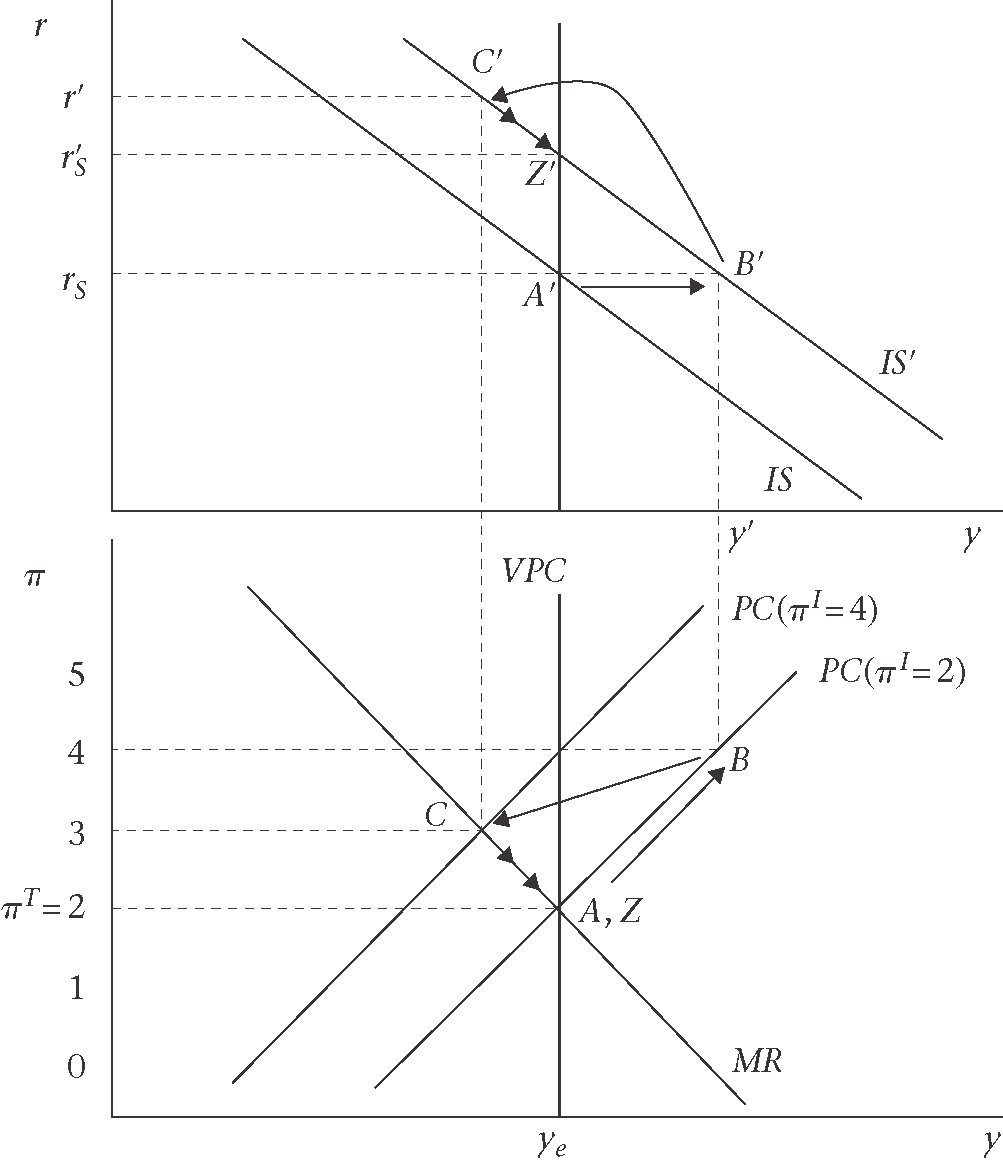
\includegraphics[width=0.5\linewidth]{Imagens/a13i3.png}
\end{figure}

\begin{figure}[H]
    \centering
    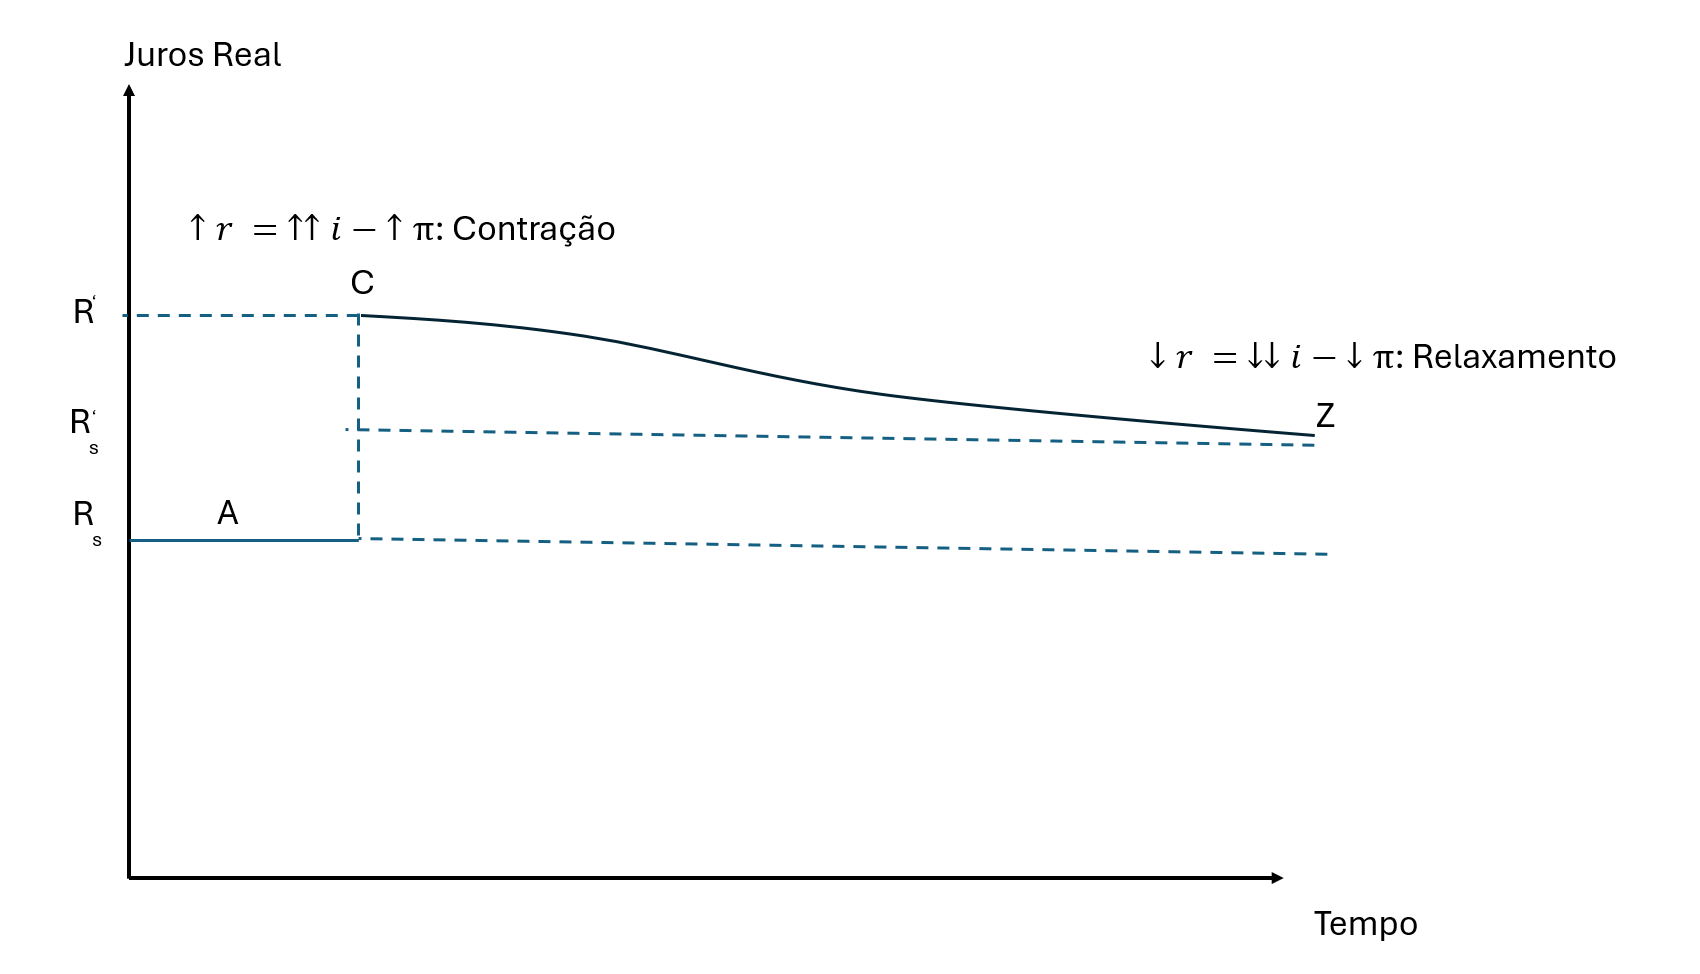
\includegraphics[width=0.7\linewidth]{Imagens/a13i7.png}
\end{figure}

O choque de demanda corrente alimenta a inflação base no período seguinte: \( \pi^I = 4\% \), deslocando \( PC \).

A diferença fundamental é que a taxa natural de juros muda \( r'_s > r_s \).

A melhor resposta do BC é uma elevação da taxa de juros: \( r' > r'_s > r_s \) com \( y < y_e \) e \( 2\% < \pi < 4\% \).

A economia transita nos pontos \( B \to C \) e \( B' \to C' \) até convergir para \( Z, Z' \).

Para um choque permanente de demanda, a resposta do Banco Central será de elevar a taxa real de juros a um nível ainda maior do que se elevaria em um caso temporário. Isso ocorre pois ele terá de combater não somente os efeitos subsequentes derivados da inércia inflacionária, mas também os efeitos do choque permanente sobre o nível de atividade. A lógica é a mesma dos exemplos anteriores, com o seguinte caminho sendo realizado:

(A \( \Rightarrow \) CHOQUE DE DEMANDA PERMANENTE \( \Rightarrow \) B \( \Rightarrow \) C \( \Rightarrow \) Z)


\subsection{\textbf{MR e Taxa Real de Juros}}

A manutenção da taxa nominal - ou mesmo da taxa real de juros - pode ser insuficiente para estabilizar \( (\pi, y) \to (\pi^T, y_e) \). Isso ocorre porque:  \begin{itemize}
    \item A manutenção de \( r = r_s \)  face a \( \pi^e > \pi^T \) exige elevar a taxa nominal na proporção do aumento da expectativa inflacionária:
    \[
    \uparrow i = r_s + \uparrow \pi^e \ \ \text{logo} \ \ \Delta i= \Delta \pi>0
    \]
    \item Como a economia permanece com \( y' > y_e \), então \( \pi^e \) e \( \pi \) continuam crescendo.
    \item Se a taxa nominal de juros \( i \) for mantida enquanto \( \pi^e > \pi^T \), ocorre uma redução da taxa real de juros:
    \[
    r \downarrow = \bar{i} - \uparrow \pi^e < r_s
    \]
    Isso gera um estímulo ainda maior na demanda agregada e acelera a inflação.
\end{itemize}

\textbf{Princípio de Taylor}: A taxa nominal de juros deve variar mais que proporcionalmente à mudança na taxa esperada de inflação:

\[
|\Delta i| > |\Delta \pi^e| \Rightarrow i = f_\pi \times (\pi - \pi^T), \quad \text{com} \quad f_\pi > 1
\]

Isso significa que a \textbf{taxa real de juros} deve subir quando a inflação está acima da meta e diminuir quando está abaixo da meta.  
Se esse princípio for violado, a inflação diverge ao invés de convergir. Ou seja, é  necessário que a taxa de real de mude para gerar o hiato do produto consistente com a convergência inflacionária.

Se houver um choque inflacionário, considere \( \Delta \pi > 0 \Rightarrow \pi > \pi^T \):

\begin{itemize}
    \item Se o BACEN estabiliza \( r = r_s \Rightarrow \Delta i = \Delta \pi > 0 \Rightarrow y - y_e = 0 \), mas \( \pi > \pi^T \).
    \item Se o BACEN estabiliza \( i \Rightarrow r < r_s \), pois \( r = i - \pi \Rightarrow y^d \Rightarrow \uparrow \uparrow \pi \).
\end{itemize}

Para evitar esse problema, o Banco Central segue a \textbf{Regra de Juros}:

\[
i = \underbrace{i_s}_{r_s-\pi^T} + f_\pi * (\pi - \pi^T)
\]

\textbf{Onde:}\begin{itemize}
    \item \( f_0 \) e \( f_\pi \) são coeficientes que explicam a determinação da taxa de juros conforme as intenções do Banco Central.
    \item Se \( f_\pi > 1 \), garante-se que \( |\Delta i| > |\Delta \pi| \), ou seja, \( |\Delta r| > 0 \), o que torna a política efetiva para aproximar a inflação à meta e o produto ao potencial.
\end{itemize}

Esse pressuposto é chamado de \textbf{Princípio de Taylor}. Segundo ele, a taxa nominal de juros deve variar mais que proporcionalmente à mudança na taxa esperada de inflação.  
Ou seja, a taxa real de juros deve:\begin{itemize}
    \item \textbf{Subir} quando a inflação está acima da meta.
    \item \textbf{Diminuir} quando a inflação está abaixo da meta.
\end{itemize}

Se o princípio for violado, a inflação divergirá da meta, mantendo-se sob um equilíbrio diferente ou oscilando para cima e para baixo.

Quando a economia se encontra na meta e com o produto em equilíbrio interno, tem-se: \begin{itemize}
    \item \( f_\pi (\pi - \pi^T) \) se iguala a zero quando a inflação corrente está na meta \( (\pi = \pi^T) \).
    \item Pela equação da regra de juros:
    \[
    i = f_0 + f_\pi * (\pi - \pi^T)
    \]
    Encontra-se que \( i = f_0 \), ou seja, \( i = i_s \).
    \item Em termos da taxa de juros real:
    \[
    r_s = i_s - \pi^T \Rightarrow i = f_0 = i_s = \pi^T + r_s
    \]
\end{itemize}

\subsection{\textbf{Desinflação e Taxa de Sacrifício}}

\textbf{Razão de Sacrifício}

A Taxa de Sacrifício ou \textbf{Razão de Sacrifício} mede os custos da desinflação, ou seja, a quantidade de desemprego cumulativo necessário para reduzir a inflação a uma proporção desejada. A definição matemática é dada por:

\[
\frac{\sum_{t=0}^{t} (y_t - y_e)}{\pi^T - \pi_0}
\]

\textbf{Exemplo:}  
Suponha \( \pi_0 = 13\% \) e \( \pi^T = 3\% \), então:

\[
\pi^T - \pi_0 = 10\%
\]

Se a estratégia de desinflação durar 5 anos, com um hiato de \( -3\% \) ao ano, a razão de sacrifício será:

\[
\frac{\sum_{t=0}^{4} (-3\%)_t}{-10\%} = \frac{15\%}{-10\%} = 1,5
\]

Isso significa que o custo necessário para diminuir um ponto percentual da inflação é de 1,5 pontos percentuais de produto.

\textbf{Regra Monetária e Impacto da Política Monetária}

A Regra Monetária é representada por:

\[
y_t - y_e = - b (\pi_t - \pi^T)
\]

onde \( b \) é o grau de aversão do Banco Central à inflação. Quando \( b \to \infty \), temos:

\[
\lim_{b \to \infty} \frac{(y_t - y_e)}{b} = -(\pi_t - \pi^T) = 0
\]

Isso implica que o Banco Central deseja reduzir a inflação o mais rápido possível, conduzindo um tratamento de choque conhecido como \textit{Cold Turkey}.

\begin{figure}[H]
    \centering
    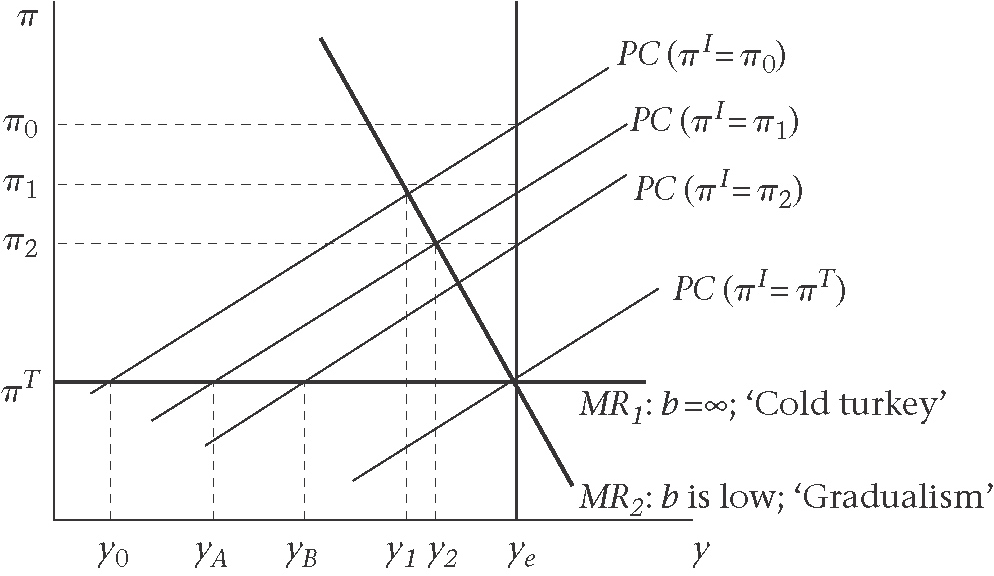
\includegraphics[width=0.7\linewidth]{Imagens/a13i5.png}
\end{figure}

\textbf{Choque vs. Gradualismo}

Duas estratégias de desinflação podem ser consideradas:\begin{itemize}
    \item \textbf{Choque}: A política monetária busca trazer a inflação à meta em um único período. O ajuste é imediato, gerando um maior impacto no desemprego a curto prazo.
    \item \textbf{Gradualismo}: A inflação converge à meta ao longo de vários períodos, reduzindo o impacto imediato no desemprego.
\end{itemize}

A razão de sacrifício sob tratamento de choque é dada por:

\[
\frac{y_0 - y_e}{\pi^T - \pi_t}
\]

Enquanto a razão de sacrifício sob gradualismo é:

\[
\frac{y_1 - y_e + y_2 - y_e + \dots}{\pi^T - \pi_t}
\]

\textbf{Curva de Phillips e Razão de Sacrifício}

Se a Curva de Phillips for \textbf{linear}, a razão de sacrifício será independente do grau de aversão do Banco Central à inflação:

\[
\pi_t = \pi_{t-1} + \alpha (y_t - y_e)
\]

Rearranjando:

\[
-\alpha (y_t - y_e) = \pi_{t-1} - \pi_t
\]

\[
\frac{1}{\alpha} = - \frac{y_t - y_e}{\pi_{t-1} - \pi_t}
\]

Se a Curva de Phillips for \textbf{não linear}, a razão de sacrifício não será constante, variando de acordo com os níveis de imediatismo ou gradualismo adotados.

\textbf{Impacto das Expectativas Inflacionárias}

Se a Curva de Phillips incluir um fator de expectativas inflacionárias, temos:

\[
\pi_t = \gamma \pi^T + (1 - \gamma) \pi_{t-1} + \alpha (y_t - y_e)
\]

Quando a meta \( \pi^T \) influencia diretamente as expectativas, a inércia inflacionária tem menor peso, permitindo uma desinflação menos custosa para o Banco Central.

\textbf{Hipótese Alternativa: Curva de Phillips Convexa}

\begin{figure}[H]
    \centering
    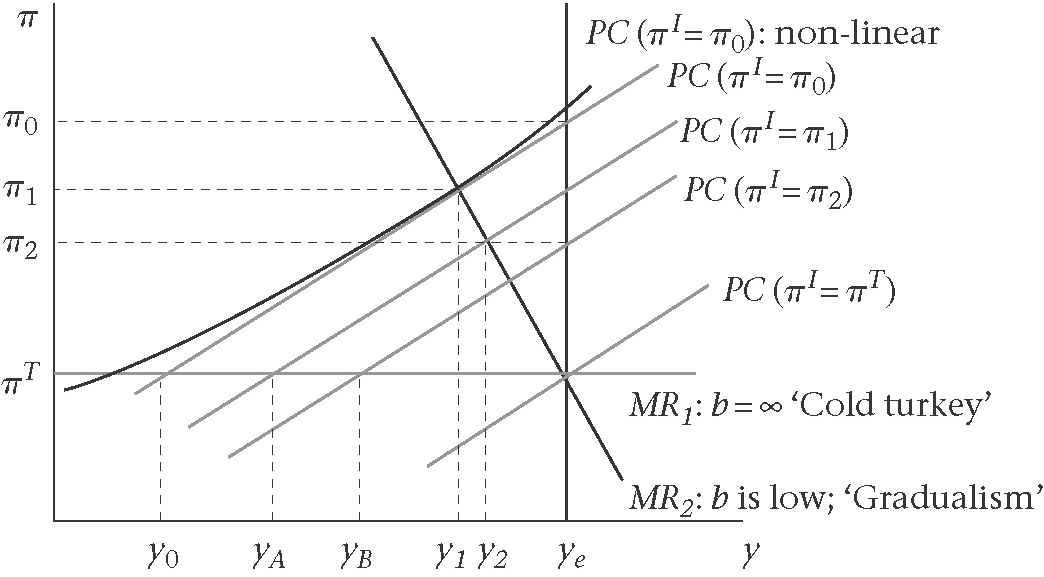
\includegraphics[width=0.7\linewidth]{Imagens/a13i6.png}
\end{figure}

Se a Curva de Phillips for convexa:

\begin{itemize}
    \item A inflação cai proporcionalmente menos para taxas de desemprego elevadas.
    \item Uma maior contração no produto é necessária para obter a mesma queda na inflação.
    \item O desemprego sob tratamento de choque será maior que sob gradualismo.
\end{itemize}

Isso implica que: desemprego acumulado sob gradualismo \(<\) desemprego com tratamento de choque

Se houver maior resistência no ajuste de preços e salários, a Curva de Phillips se torna mais horizontal, aumentando a taxa de sacrifício.

Considere uma Curva de Phillips na qual as expectativas inflacionárias incorporam tanto a meta de inflação quanto a inflação passada, de modo que
\[
\pi_t \;=\; \gamma \,\pi^T \;+\; (1-\gamma)\,\pi_{t-1} \;+\; \alpha \,(y_t - y_e).
\]
Nesse contexto, se a meta de inflação (\(\pi^T\)) participar explicitamente da formulação das expectativas, a inércia inflacionária (representada por \(\pi_{t-1}\)) perde parte de sua importância. Isso implica maior velocidade de convergência da inflação em direção à meta, pois o peso da inércia é reduzido. Em outras palavras, com a meta inserida diretamente na curva, o \emph{custo de desinflação} (em termos de hiato de produto necessário) tende a ser menor.

Ou seja, para o Banco Central, fica menos custoso, em termos de movimentação do produto, promover a convergência da inflação à meta. A inércia inflacionária funciona como o principal fator de resistência na mudança da taxa de inflação: quanto maior for o peso atribuído à inflação passada, mais difícil é alterar a inflação corrente. Portanto, quando esse peso se torna menor (ou quando a meta de inflação ganha maior relevância), a resistência diminui, e o processo de redução inflacionária se torna menos oneroso para a economia.

Vou colocar a foto da minha arara no site do black

 \newpage
\section{\textbf{Mercado de trabalho e oferta}}

Iremos agora investigar alterações que podem ocorrer no mercado de trabalho, e o seu papel na geração de flutuações na oferta real de bens e serviços. Essas flutuações, relacionadas à PS (\emph{Price Setting}) e à WS (\emph{Wage Setting}), podem ser:

\[
\text{PS} \begin{cases}
\text{impostos} \\
\text{concorrência no mercado de bens} \\
\text{regulação da competição} \\
\text{proteção comercial}
\end{cases}
\quad\text{e}\quad
\text{WS} \begin{cases}
\text{seguro desemprego} \\
\text{salário mínimo} \\
\text{legislação sindical/trabalhista} \\
\text{políticas de renda}
\end{cases}
\]

Assim, iremos observar como o Banco Central deve reagir para algumas dessas mudanças institucionais no mercado de trabalho, já que essas têm repercussões na determinação de preços e salários e, portanto, na forma de condução das políticas monetárias.

Lembrando a definição da taxa natural de desemprego:
\[
U_{\text{ICE}} 
= \frac{L - E_{\text{ICE}}}{L} 
= \frac{U_{\text{ICE}}}{L} 
= \text{NAIRU},
\]
onde NAIRU é a \emph{Non-Accelerating Inflation Rate of Unemployment}. E que
\[
y_e = f(E_{\text{ICE}}),
\]
ou seja, a produção potencial depende do nível de emprego de equilíbrio.

Lembre-se também que:
\begin{itemize}
    \item \textbf{Choques de demanda} (em $y_t$) induzem movimentações ao longo da Curva de Phillips (PC).
    \item \textbf{Choques de oferta} (em $y_e$) afetam o produto potencial, deslocando tanto a Regra Monetária (MR) quanto a própria PC.
\end{itemize}

\subsection{\textbf{Estrutura da Oferta, Políticas e Choques}}

As alterações em PS e WS (por exemplo, redução do poder de barganha dos trabalhadores, mudanças em impostos, legislação, protecionismo etc.) podem deslocar a estrutura de oferta, afetando simultaneamente a taxa de desemprego de equilíbrio (NAIRU), o produto potencial ($y_e$) e, por consequência, a condução da política monetária.

A taxa de equilíbrio (ou natural) de desemprego não permanece constante ao longo do tempo, pois choques estruturais podem alterar a oferta da economia ao deslocar \textbf{WS} (Wage Setting), \textbf{PS} (Price Setting) ou ambas.

\[
\begin{array}{c}
\text{políticas de oferta} \\
\text{instituições do mercado de trabalho}
\end{array}
\quad
\Bigg\} 
 \Longrightarrow 
\Delta WS \text{ e } \Delta PS
 \Longrightarrow 
\Delta \text{taxa de desemprego de equilíbrio}
\]

\[
\Delta \text{taxa de desemprego de equilíbrio} 
\Longrightarrow
\Delta \text{Curva de Phillips} 
\Longrightarrow 
\Delta \text{Regra Monetária}
\]

Portanto,

\[
\Delta \text{condições de oferta} 
 \Longrightarrow 
\Delta \text{produto e emprego de equilíbrio} 
 \Longrightarrow 
\Delta \text{função de reação do Banco Central}
\]

\subsubsection{\textbf{Exemplo: Redução do poder de barganha dos trabalhadores (WS para baixo)}}

\begin{figure}[H]
    \centering
    \includegraphics[width=0.7\linewidth]{Imagens/a14i3.png}
\end{figure}

Considere-se um choque exógeno no poder de barganha, devido, por exemplo, a mudanças na legislação trabalhista que reduzam a influência de sindicatos. Nesse caso, a relação salarial (WS) pode ser representada de forma simplificada por
\[
\frac{W^{ws}}{P} = b(E,\,z),
\]
onde $z$ representa fatores exógenos que afetam negativamente o poder de barganha dos trabalhadores (por exemplo, leis menos favoráveis à negociação sindical). Se houver um choque que reduza $z$, isso desloca a curva WS para baixo:
\[
\downarrow z \;\Longrightarrow\; \text{WS desloca para baixo} \;\Longrightarrow\; (\downarrow W^{ws} = P^e \times \downarrow b).
\]

\textbf{Consequências diretas no emprego e salários:}
\begin{itemize}
    \item Para o mesmo salário real, os trabalhadores podem ofertar mais trabalho ou aceitar um salário real mais baixo.
    \item O emprego de equilíbrio tende a aumentar (se a curva PS não for perfeitamente horizontal).
    \item O salário real de equilíbrio tende a se reduzir ou, em alguns casos, permanecer inalterado (dependendo de quão elástica for a PS).
\end{itemize}

\textbf{Efeitos macroeconômicos e a resposta do Banco Central:}
\begin{itemize}
    \item Com a WS deslocada para baixo, o custo de produção por unidade de trabalho pode diminuir, reduzindo a inflação de custos no curto prazo.
    \item Dado que a inflação efetiva $\pi_t$ pode ficar abaixo da meta $\pi^T$, o Banco Central (BC) tende a afrouxar a política monetária (reduzir $r_s$) para estimular a demanda até o novo nível potencial de produto $y_e'$.
    \item Em termos de Curva de Phillips, o produto potencial $y_e$ aumenta, deslocando a PC:
    \[
      \pi_t = \pi_{t-1} + \alpha (y_t - \uparrow y_e).
    \]
    \item No novo equilíbrio, a taxa de desemprego natural (NAIRU) é menor e a inflação pode se estabilizar na meta, caso a política monetária seja bem calibrada.
\end{itemize}

\begin{figure}[H]
    \centering
    \includegraphics[width=0.7\linewidth]{Imagens/a14i1.png}
\end{figure}

\subsubsection{\textbf{Dinâmica do Ajuste: Pontos A, B, C e Z}}

Para ilustrar o impacto de um choque favorável de oferta (em WS) na trajetória da inflação, imagine que a economia se encontra inicialmente em um equilíbrio interno no ponto A. O choque exógeno no poder de barganha dos trabalhadores faz com que estes aceitem salários menores, reduzindo temporariamente o nível de consumo (menor renda) e, consequentemente, a inflação. A oferta de trabalhadores de equilíbrio se torna maior para um salário real não tão alterado, deslocando a curva WS para a direita e surgindo um novo nível de emprego de equilíbrio competitivo imperfeito ($E_{\text{ICE}}'$). Nesse movimento inicial, a inflação efetiva pode ficar abaixo da meta (por exemplo, 2\% em vez de 4\%), e o produto efetivo ainda não alcança o novo potencial ($y_e' > y_e$). Para corrigir esse duplo desequilíbrio, o BC reduz a taxa real de juros e eleva o nível de produto (fase B $\to$ C), mas a inflação permanece abaixo da meta. Em seguida, para trazer a inflação de volta a $\pi^T$, o BC mantém a taxa de juros em nível baixo por mais tempo ou induz pequeno hiato positivo de produto, estimulando gradualmente o aumento de preços até a meta, levando a economia ao ponto Z ou Z'. No fim do processo, o novo equilíbrio interno corresponde a $y = y_e'$ e $\pi = \pi^T$.

\textbf{Conclusões gerais do ajuste:}
\begin{itemize}
    \item Em um choque de oferta favorável (redução exógena do poder de barganha), a WS se desloca para baixo/direita, aumentando o emprego e reduzindo a inflação no curto prazo.
    \item A inflação abaixo da meta e o produto aquém do novo potencial configuram um duplo desequilíbrio inicial.
    \item O Banco Central reduz a taxa de juros, aproximando o produto do novo $y_e'$. Para trazer a inflação de volta à meta, pode manter a taxa de juros baixa e criar hiato de produto positivo por algum período.
    \item Ao final do processo, a taxa de desemprego é menor (NAIRU diminui), o produto potencial se eleva ($y_e' > y_e$) e a inflação retorna à meta.
\end{itemize}

\begin{figure}[H]
    \centering
    \includegraphics[width=0.7\linewidth]{Imagens/a14i2.png}
\end{figure}


\textbf{Choque de oferta, regra monetária e deslocamentos da Curva de Phillips}

A figura mostra como um choque de oferta pode alterar a regra monetária, passando de MR para MR'. Isso afeta a Curva de Phillips (PC) em diferentes horizontes de tempo:

\begin{itemize}
    \item \textbf{No curto prazo}, a PC pode partir de um estado com \(\pi^T = 4\%\) e \(y_e\), depois deslocar-se para uma nova combinação \(\pi^T = 4\%\) e \(y_e'\) e, em seguida, chegar a \(\pi^T = 2\%\) e \(y_e'\). Esse movimento reflete tanto a queda temporária da inflação quanto o aumento do produto potencial devido ao choque de oferta.
    \item \textbf{No médio ou longo prazo}, a PC pode evoluir de \(\pi^T = 2\%\) e \(y_e\) para \(\pi^T = 4\%\) e \(y_e\). Nesse momento, as condições macroeconômicas retornam ao alvo de inflação de 4\%, enquanto o produto potencial se consolida no patamar associado a \(y_e\). Além disso, a variação de preços e custos (VPC) pode se deslocar para a direita em razão do novo equilíbrio de oferta.
\end{itemize}

\begin{figure}[H]
    \centering
    \includegraphics[width=0.7\linewidth]{Imagens/a14i4.png}
\end{figure}

O diagrama também destaca que o choque de oferta altera a taxa real de juros que estabiliza o produto e a inflação (ou seja, \(\,r_s\) passa a \(\,r_s' < r_s\)), permitindo uma demanda maior compatível com o novo nível de produto potencial e a inflação-alvo. Em outras palavras, a regra monetária (MR) se ajusta para MR', adequando a política de juros às novas condições de oferta, inflação e produto.

\subsection{\textbf{Deslocamentos de WS e PS}}

Mudanças na taxa de desemprego de equilíbrio podem resultar de pressões salariais (que afetam a WS) ou de pressões sobre os preços (que afetam a PS). A seguir, discute-se como a mensuração de preços e salários — em termos nominais e reais — interfere nesses deslocamentos, bem como os principais tipos de choques que deslocam cada curva.

\subsubsection{\textbf{Mensuração de preços e salários: nominais e reais}}

Os preços ao consumidor, denotados por \(P_c\), refletem os preços ao produtor (\(P\)) acrescidos de tributação indireta, \(t_v\). Assim:
\[
P_c = P \,(1 + t_v).
\]
Impostos indiretos (por exemplo, IPI, ICMS) incidem sobre transações de mercadorias e serviços.

O salário nominal recebido pelos trabalhadores, \(W\), já é líquido de impostos e contribuições previdenciárias; em outras palavras, é o valor que eles efetivamente recebem. Entretanto, para analisar poder de compra e custos de produção, consideramos:

- \emph{Salário real relevante para o trabalhador}: 
  \[
    \frac{W}{P_c},
  \]
  que mede o poder de compra efetivo em termos dos preços ao consumidor.

- \emph{Salário real relevante para a empresa}:
  \[
    \frac{W \,(1 + t_d)}{P},
  \]
  onde \(t_d\) representa os tributos diretos sobre a folha (ou outras incidências pagas pela firma). Esse salário real indica o custo efetivo para a empresa, pois é o salário nominal bruto pago (incluindo impostos) em relação ao preço ao produtor.

Combinando essas definições, surgem expressões que incorporam tanto a margem de lucro (\(\mu\)) quanto as alíquotas de impostos diretos e indiretos. Se
\[
P = \frac{1}{\,1-\mu\,},
\]
então
\[
P_c = P \,(1 + t_v) = \frac{1 + t_v}{\,1-\mu\,}.
\]
Da mesma forma, o salário real do trabalhador em relação a \(P_c\) e o custo salarial para a empresa em relação a \(P\) podem exibir uma diferença chamada \emph{cunha fiscal}, responsável por divergências entre o salário real recebido pelos trabalhadores e o salário real efetivamente pago pelas empresas. Um aumento dessa cunha tende a deslocar a PS para baixo, elevando o desemprego de equilíbrio.

\subsubsection{\textbf{Choques sobre os preços (PS)}}

Em termos gerais, podemos representar a condição de fixação de preços (PS) por:
\[
\frac{W}{P_c} \;=\; \lambda\,f(\mu,\,z_p),
\]
onde \(z_p\) é um vetor de fatores que impactam o \emph{markup} ou a produtividade, afetando assim a determinação de preços. Exemplos de choques em \(z_p\):
- Maior produtividade (\(\Delta A > 0\)) eleva \(\lambda\) ou reduz custos.  
- Maior competição/menor markup (\(\Delta\mu < 0\)).  
- Redução da cunha fiscal (\(\downarrow t_v\) ou \(\downarrow t_d\)).  

Esses fatores podem deslocar a PS para cima (aumentando o salário real de equilíbrio) ou para baixo.

\subsubsection{\textbf{Choques sobre os salários (WS)}}

De modo análogo, podemos representar a condição de formação salarial (WS) por:
\[
\frac{W}{P_c} = b(E,\,z_w),
\]
onde \(z_w\) é um vetor de fatores que impactam o salário nominal (ex.: poder sindical, seguro-desemprego etc.). Exemplos de choques em \(z_w\):
- Diminuição dos benefícios de seguro-desemprego.  
- Enfraquecimento dos sindicatos.  
- Legislação trabalhista mais flexível.  

Tais mudanças deslocam a WS para baixo, aumentando o emprego de equilíbrio e reduzindo o salário real de equilíbrio (ou vice-versa).

\subsubsection{\textbf{Produtividade}}

Pode ser adequado incluir um parâmetro de produtividade na curva WS, por exemplo:
\[
\frac{W}{P_c} = \lambda \, b(E,\,z_w)
\quad \text{ou} \quad
\frac{W}{P_c} = b(\lambda,\,E,\,z_w).
\]
Se a produtividade \(\lambda\) cresce continuamente, mas o desemprego não diminui, pode ser que as demandas salariais estejam crescendo em linha com a produtividade, mantendo a taxa de desemprego de equilíbrio relativamente estável. Porém, se a percepção de mudanças na tendência de produtividade ocorrer de forma rápida, o impacto sobre o desemprego (e, inicialmente, sobre o salário real) pode ser maior, especialmente se houver defasagens entre ajustes de PS e WS.

\subsubsection{\textbf{Considerações finais}}

O crescimento contínuo da produtividade sem queda do desemprego sugere que a WS incorpore a produtividade de forma quase proporcional; entretanto, na prática, a dinâmica salarial é mais complexa, pois há defasagens e, muitas vezes, os choques afetam primeiro a PS e, só depois, as negociações salariais. Isso ajuda a explicar tanto períodos em que países desenvolvidos apresentaram maior ou menor desemprego nos anos 1970--80 quanto o crescimento do emprego nos EUA nos anos 1990, associado a mudanças tecnológicas e institucionais.

\newpage
\section{\textbf{Política Monetária}}

\subsection{\textbf{Paradigmas para a análise dos tipos de política monetária}}

Ao longo dos últimos séculos, os processos de ajuste da economia em equilíbrio de longo prazo envolveram as funções IS e LM. O instrumento central de política monetária era a quantidade de moeda em circulação.

Atualmente, adota-se outra metodologia para abordar os ajustes da economia no equilíbrio de longo prazo: a regra monetária (\textbf{RM}). Assim, o instrumento central de política monetária desse modelo é a regulação da taxa nominal de juros de curto prazo, guiada por regras de juros que traçam as melhores respostas do Banco Central aos diferentes tipos de desvios do equilíbrio interno.

\subsection{\textbf{Paradigmas alternativos}}

\subsubsection{\textbf{LM}}
O nível de preços e a taxa de inflação são determinados pela oferta de moeda. O principal instrumento da política monetária nesse modelo é a oferta monetária. O processo de ajuste da economia é guiado pela interação entre o mercado de bens (IS) e ativos (LM), acrescido da Curva de Phillips (PC).

\subsubsection{\textbf{RM}}
O nível de preços e a taxa de inflação são determinados pela política macroeconômica. O principal instrumento da política monetária passa a ser a taxa nominal de juros de curto prazo. Assim, o mecanismo de ajuste da economia é guiado pela \emph{regra de juros}.

\subsection{\textbf{A regra de política monetária}}

A política do Banco Central depende dos seguintes parâmetros:
\begin{itemize}
    \item A meta inflacionária: \(\pi^T\)
    \item As preferências do Banco Central: \(\beta\)
    \item A inclinação da Curva de Phillips (CP): \(\alpha\)
    \item A sensibilidade da demanda agregada à taxa real de juros: \(a\)
    \item O nível do produto de equilíbrio (natural): \(y_e\)
    \item A taxa real de juros (natural) que estabiliza o produto: \(r_s\)
\end{itemize}

A relação entre a taxa de juros real e o produto segue:
\[
r_s \longrightarrow y_e \longrightarrow y^d(r_s).
\]

\subsubsection{\textbf{Função de Perdas do Banco Central}}

O Banco Central busca minimizar as perdas econômicas associadas a desvios da inflação em relação à meta e a desvios do produto em relação ao equilíbrio. A função de perdas é expressa como:
\[
L = (y_t - y_e)^2 + \beta \, (\pi_t - \pi^T)^2.
\]

A razão para modelar as perdas em forma quadrática reside na simplicidade algébrica e na simetria da penalização de desvios tanto da inflação quanto do produto. Essa formulação facilita a minimização da função de perdas e a definição da melhor resposta da política monetária.

A interpretação da função de perdas é a seguinte:
\begin{itemize}
    \item Se \(\beta = 0\), a inflação é irrelevante para o Banco Central, que apenas minimiza desvios do produto (\(y_t = y_e\)).
    \item Se \(0 < \beta < \infty\), tanto inflação quanto produto são considerados.
    \item Se \(\beta = 1\), o Banco Central dá igual importância a ambos os desvios.
    \item Se \(\beta \to \infty\), o Banco Central prioriza exclusivamente a estabilidade da inflação, tornando desvios do produto irrelevantes.
\end{itemize}

\subsubsection{\textbf{Representação gráfica das preferências do Banco Central}}

A função de perdas permite ilustrar as preferências do Banco Central geometricamente:
\begin{itemize}
    \item \(\beta = 1\): O Banco Central se preocupa igualmente com desvios da inflação e do produto. A curva de indiferença tem formato circular, e o bem-estar econômico melhora conforme o círculo diminui.
    \item \(\beta > 1\): O Banco Central é mais sensível a desvios da inflação. A curva de indiferença assume forma elíptica com eixo maior horizontal. Se \(\beta \to \infty\), a curva de indiferença coincide com a linha \(\pi = \pi^T\).
    \item \(\beta < 1\): O Banco Central prioriza a estabilidade do produto. A curva de indiferença é uma elipse com eixo maior vertical. Se \(\beta = 0\), a curva de indiferença se torna uma linha sobre \(y = y_e\).
\end{itemize}

\begin{figure}[H]
    \centering
    \includegraphics[width=0.7\linewidth]{Imagens/a14i5.png}
\end{figure}

\subsection{\textbf{A Regra de Política Monetária}}
\begin{figure}[H]
    \centering
    \includegraphics[width=0.7\linewidth]{Imagens/a15i1.png}
\end{figure}

O Ponto A representa uma completa acomodação : Inflação e Produto Inalterado. O Ponto C representa nenhuma acomodação : Inflação na meta ao custo de queda do produto. As perdas são minimizadas no ponto intermediário D, que é a tangência de \(L\) com \(PC\).

Lembre-se que a \textbf{escolha ótima} vai definir a coleção de pontos que sobre a regra monetária combinam o que se pode fazer e o que se deseja fazer. Assim, lembra-se que a curva de Phillips traça apenas aqueles pontos que são factíveis.

\[
\min L = (y_t - y_e)^2 + \beta \cdot (\pi_t - \pi^T)^2 \rightarrow \text{Desejável ; preferências}
\]
\[
s.a \ \ \pi_t=\pi_{t-1}+\alpha(y_t-y_e) \rightarrow \text{restrição ;  factível(PC)}
\]

Dessa forma, substitui-se $\pi_t$ pela curva de Phillips:

\[
\min_{\{y_t\}} L = (y_t - y_e)^2 + \beta \cdot (\underbrace{\pi_{t-1} + \alpha \cdot (y_t - y_e)}_\text{Curva de Phillips} - \pi^T)^2
\]

Assim, para encontrar a condição de primeira ordem, deriva-se essa função de minimização e iguala a zero:

\[
\text{C.P.O.} \rightarrow 2 \cdot (y_t - y_e) + 2\beta \cdot \alpha \cdot (\underbrace{\pi_{t-1} + \alpha \cdot (y_t - y_e)}_\text{Curva de Phillips} - \pi^T) = 0
\]

\textbf{Essa equação (CPO) é aquela que torna os custos marginais iguais aos benefícios marginais!}

Assim, dessa função, encontra-se a Regra Monetária, o que expressa justamente o seu propósito como descrito acima:

\[
2 \cdot (y_t - y_e) + 2\alpha \beta \cdot (\pi_t - \pi^T) = 0
\]

\[
\underbrace{y_t - y_e}_{CM_g} = \underbrace{-\overbrace{\alpha \beta}^{b} \cdot (\pi_t - \pi^T)}_{BM_g}
\]

\[
y_t - y_e = -b \cdot (\pi_t - \pi^T) \rightarrow (\textit{REGRA MONETÁRIA})
\]

Assim, percebe-se que: \( b = \alpha \cdot \beta \).
\begin{figure}[H]
    \centering
    \includegraphics[width=0.7\linewidth]{Imagens/a15i2.png}
\end{figure}

Como observar a diferenciação total da função de perdas descrita? Qual a inclinação da circunferência de indiferença?

Quanto é \(\left(\frac{d\pi}{dy}\right)_{\bar{L}} \)?

\[
d\bar{L} = 0 = 2(y_t - y_e) * dy + 2\beta (\pi_t - \pi^T) * d\pi
\]

\[
TMS_{y,\pi} = \left(\frac{d\pi}{dy}\right)_{\bar{L}} = -\frac{1}{\beta} * \frac{(y_t - y_e)}{(\pi_t - \pi^T)} \rightarrow \textbf{INCLINAÇÃO DA FUNÇÃO DE INDIFERENÇA}
\]

Essa inclinação é a conhecida Taxa Marginal de Substituição (TMS), representando a quantidade de produto que o Banco Central está disposto a distanciar do pleno emprego para obter uma dada aproximação da inflação à meta. Pensa-se em uma relação marginal de troca entre desvios no produto e na inflação.

Assim, sob essa circunferência de indiferença, traça-se a PC e a MR:

\begin{figure}[H]
    \centering
    \includegraphics[width=0.7\linewidth]{Imagens/a15i3.png}
\end{figure}

Combinações factíveis \(\rightarrow\) Têm de estar, para uma dada inércia inflacionária, sobre a PC

Pontos que minimizam as perdas \(\rightarrow\) Têm de estar sob a circunferência de indiferença

Coleção dos pontos que satisfazem a condição de primeira ordem \((C_{mg} = B_{mg})\), que igualam TMT com TMS \(\rightarrow\) Tem de estar sobre a Regra Monetária

Ponto Ótimo \(\rightarrow\) Ponto em que a Taxa Marginal de Substituição (TMS) é igual à Taxa Marginal de Transformação (TMT):

\[
TMT_{y,\pi} = \left(\frac{d\pi}{dy}\right)_{PC} = \alpha
\]

Essa taxa marginal de transformação representará a sensibilidade das trocas entre inflação e hiato de produto no mercado. É a inclinação da curva de Phillips.

\[
TMS_{y,\pi} = TMT_{y,\pi} \rightarrow \alpha = -\frac{1}{\beta} * \frac{(y_t - y_e)}{(\pi_t - \pi^T)} \rightarrow (\textit{REGRA MONETÁRIA})
\]

O Banco Central irá escolher a combinação de pontos que: tangenciam a dada Curva de Phillips (com dada inércia inflacionária) com a circunferência de indiferença que apresenta o menor raio.

Veja o exemplo:

\begin{figure}[H]
    \centering
    \includegraphics[width=0.7\linewidth]{Imagens/a15i5.png}
\end{figure}

\textbf{PERGUNTA: “A” é desejável?}

Em “A”, tem-se produto igual ao pleno emprego e inflação acima da meta.

R: Não! Embora “A” seja factível, por estar sobre a PC, não é desejável, pois não tangencia a circunferência da função de perdas. Nesse caso a TMT (\(\alpha\)) é maior que a TMS (\(= 0\)), ou seja, vale a pena contrair o produto para obter menor inflação.

\[
TMS = - \frac{1}{\beta} * \frac{(y_t - y_e)}{(\pi_t - \pi^T)} = - \frac{1}{\beta} * \frac{(0)}{\pi_t - \pi^T} = 0
\]

\textbf{PERGUNTA: “C” é desejável?}

Em “C”, tem-se inflação na meta e produto abaixo do pleno emprego.

R: Não! Embora “C” também seja factível, por estar sobre a PC, não é desejável, pois não tangencia a circunferência da função de perdas. Nesse caso, a TMS (\(\infty\)) é maior que a TMT (\(\alpha\)), ou seja, vale a pena estimular o produto às custas de alguma elevação na inflação.

\[
TMS = - \frac{1}{\beta} * \frac{(y_t - y_e)}{(\pi_t - \pi^T)} = - \frac{1}{\beta} * \frac{(y_t - y_e)}{(0)} = \infty
\]

\textbf{PERGUNTA: “D” é desejável?}

Em “D”, tem-se inflação acima da meta e produto abaixo do pleno emprego.

R: Sim! “D” é factível, pois está sobre PC, e é desejável, pois tangencia a circunferência de indiferença de perdas. Nesse caso, como o ponto está sobre a Regra Monetária, a TMS é igual à TMT, ou seja, não vale a pena estimular ou desestimular o produto às custas de variações na inflação. Neste caso, com \(y_1 < y_e\), o hiato do produto é negativo, o que implica em uma desaceleração inflacionária, com ajustes salariais que farão com que, ao longo das mudanças da inércia inflacionária, o equilíbrio interno seja reestabelecido.

\[
TMT = TMS = \alpha = - \frac{1}{\beta} * \frac{(y_1 - y_e)}{3 - \pi^T}
\]

\textbf{O que acontece quando o $\beta$ for mais elevado?}

R: À medida que o $\beta$ se torna maior, o Banco Central se torna mais conservador quanto a desvios inflacionários, sendo mais tolerante a divergências ao hiato do produto e menos tolerante a divergências da inflação à meta inflacionária.

Pela Regra Monetária:

\[
(\pi_t - \pi^T) = - \downarrow{\frac{1}{\alpha \uparrow{\beta}}} * (y_t - y_e)
\]

O que graficamente mostra-se por uma diminuição da inclinação da Regra Monetária, ficando mais horizontal. Isso significa que o Banco Central está disposto a sacrificar mais produto para encontrar a inflação à meta mais rapidamente.

A taxa de inflação ótima neste cenário estará sempre mais próxima da meta do que o produto estará do pleno emprego.

\begin{figure}[H]
    \centering
    \includegraphics[width=0.7\linewidth]{Imagens/a15i6.png}
\end{figure}

Supondo $\alpha = \beta = 1$, a função de reação que estabelece a regra monetária ótima toma a forma

\[
(y_t - y_e) = - (\pi_t - \pi^T)
\]
\begin{itemize}
    \item  Relação inversa entre $\pi$ e $y$ com inclinação \(-45^\circ\)
    \item  Intermediária entre completa acomodação e nenhuma acomodação
    \item  Sintetiza a relação entre a escolha do produto e a taxa de inflação associada
    \item  Minimiza as perdas dadas as preferências do BC e as restrições com que se depara
\end{itemize}

\begin{figure}[H]
    \centering
    \includegraphics[width=0.5\linewidth]{Imagens/a15i7.png}
\end{figure}


A inclinação da regra monetária define o grau de acomodação da política monetária:\begin{itemize}
    \item  \textbf{Completa acomodação}: \textit{RM} vertical com inflação e produto inalterados
    \item  \textbf{Nenhuma acomodação}: \textit{RM} horizontal com inflação na meta ao custo de queda no produto
    \item  Depende da aversão à inflação e da resposta da inflação a variações no produto
    \item  Quanto maior aversão à inflação, menos inclinado o foco da elipse de perdas
    \item  Quanto maior resposta dos salários a variações do emprego, mais inclinada a curva de Phillips
    \item  Quanto maiores $\alpha$ e/ou $\beta$, menos inclinada a \textit{RM}
\end{itemize}
\[
(\pi_t - \pi^T) = \frac{-1}{\alpha \beta} (y_t - y_e)
\]

\begin{figure}[H]
    \centering
    \includegraphics[width=0.7\linewidth]{Imagens/a15i8.png}
\end{figure}


Quanto maior $\alpha$, mais inclinada a \textit{CP}

Com $\alpha > 1$, o banco central obtém uma redução mais expressiva na inflação (comparado ao caso $\alpha = 1$) para qualquer dada redução no produto e emprego.

O custo marginal da desinflação diminui, facilitando a vida do Banco Central:\begin{itemize}
    \item Favorece estratégia mais agressiva
    \item \textit{RM}$(\alpha > 1)$ mais horizontal
\end{itemize}

Para um cenário no qual o Banco Central é igualmente tolerante aos desequilíbrios, uma Curva de Phillips mais inclinada significa que ele terá uma “estrada mais tranquila” para levar a inflação à meta, com custos menores em produto e com velocidade maior de desinflação. Assim, fatores que elevem o “α” irão tornar mais fácil para o Banco Central levar a inflação à meta. De forma análoga, quanto maior o alfa, maior a resposta da inflação ao hiato e, então mais fácil se torna levar a inflação à meta, ou seja, o benefício marginal da desinflação se torna maior. Assim, como esse benefício marginal se torna maior, acaba valendo mais a pena o Banco Central ser MAIS AGRESSIVO e, portanto, a Regra Monetária se torna mais horizontal quando se tem um aumento do alfa. 

\textbf{Resumo da Resposta:} Uma inflação mais sensível ao hiato significa que se gasta menos em desvios no produto para realizar a desinflação, facilitando uma postura mais agressiva do Banco Central nessa desinflação.  

\begin{figure}[H]
    \centering
    \includegraphics[width=0.7\linewidth]{Imagens/a15i9.png}
\end{figure}

Em síntese, como

\[
(y_t - y_e) = -\alpha \beta \left(\pi_t - \pi^T\right) \Rightarrow \pi_t - \pi^T = \frac{-1}{\alpha \beta} (y_t - y_e)
\]

Quanto maior $\alpha \beta$, menos inclinada a função de reação \textit{MR}.


\begin{figure}[H]
    \centering
    \includegraphics[width=0.7\linewidth]{Imagens/a15i10.png}
\end{figure}

\subsection{\textbf{Papel das Defasagens}}

\textbf{Agora, iremos adicionar mais um grau de profundidade nas análises, avaliando o papel das defasagens nas equações estudadas:}

Dado um choque permanente de demanda (voltar no caderno, se necessário):

Originalmente, teríamos um deslocamento da curva IS permanentemente para a direita, seguido de uma resposta do Banco Central ao choque de demanda com uma elevação da taxa de juros, o que levaria a um reestabelecimento do equilíbrio interno. A única diferença aqui é que podemos não assumir que o Banco Central reaja prontamente. Observe a seguir como funcionaria a cronologia da reação, se o Banco Central reagir prontamente.

\begin{itemize}
    \item Em t=0: Choque ocorre, IS se desloca para a direita, A$\rightarrow$B. Banco Central usa a MR para estabelecer a combinação ótima de produto e inflação $(\pi, y)$. Banco Central usa a IS para descobrir a taxa real de juros que ratifica a combinação $(\pi, y)$ escolhida. Assim, Banco Central reage ao choque, elevando a taxa de juros, ainda sobre B.
    \item Em t=1: Se observa o efeito da reação do Banco Central na IS, ou seja, o produto contrai, B$\rightarrow$C.
    \item Em t=2: Equilíbrio é restabelecido, agora sob uma taxa de juros mais alta, C$\rightarrow$Z.
\end{itemize}

\begin{figure}[H]
    \centering
    \includegraphics[width=0.7\linewidth]{Imagens/a15i11.png}
\end{figure}

\subsection{\textbf{Uma Regra de Juros - à la Taylor}}

Deriva-se, portanto, uma regra de juros em termos do estado da economia, partindo das equações PC, MR e IS:

\begin{align}
\text{(1) MR:} \quad & \pi_1 - \pi^T = -\frac{1}{\alpha \beta} \cdot (y_t - y_e) \\
\text{(2) PC:} \quad & \pi_0 + \alpha \cdot (y_t - y_e) - \pi^T = -\frac{1}{\alpha \beta} \cdot (y_1 - y_e) \\
\text{(3) IS:} \quad & y_1 - y_e = -a \cdot (r_0 - r_s)
\end{align}

\textbf{Obs.:} Lembre que “$a$” irá representar a eficiência das políticas monetárias em oscilar o produto por variações na taxa de juros.

\[
\pi_0 - \pi^T = -\left( \alpha + \frac{1}{\alpha \beta} \right) \cdot (y_1 - y_e)
= a \cdot \left( \alpha + \frac{1}{\alpha \beta} \right) \cdot (r_0 - r_s)
\]

\textbf{Resultando em uma REGRA DE JUROS EM TERMOS REAIS:}

\[
r_0 = r_s + \frac{1}{a \cdot \left( \alpha + \frac{1}{\alpha \beta} \right)} \cdot (\pi_0 - \pi^T)
\]

\textbf{Interpretação:} A taxa real de juros hoje será maior/igual/menor em relação à taxa real de juros neutra (\( r_s \)) se a distância da inflação hoje à meta for maior/igual/menor que zero.

Em uma Regra de Juros em Termos Reais, para que o Princípio de Taylor seja satisfeito, é apenas necessário que a variação \( |\Delta r| \) seja maior que 0.

Assim, tratando essa equação em uma \textbf{REGRA DE JUROS EM TERMOS NOMINAIS}, fica:

\begin{align*}
r_0 + \pi_0 &= r_s + \pi^T + \pi_0 - \pi^T + \frac{1}{a \cdot \left( \alpha + \frac{1}{\alpha \beta} \right)} \cdot (\pi_0 - \pi^T) \\
i_0 &= i_s + \underbrace{\left[ 1+ \frac{1}{a \cdot \left( \alpha + \frac{1}{\alpha \beta} \right)} \right]}_{>1} \cdot (\pi_0 - \pi^T)
\end{align*}

Perceba que o termo em verde pode ser utilizado para avaliar a validade do Princípio de Taylor (\( |\Delta i| > |\pi_t| \)), tal que quando esse termo for maior do que 1, o Princípio de Taylor será satisfeito.

Interpreta-se:

\begin{itemize}
  \item \( \uparrow \beta \) = Maior intolerância do Banco Central a desequilíbrios inflacionários \( \Rightarrow \) ajuste mais forte na taxa de juros. Caso \(\beta \rightarrow 0\) a MR estará sobreposta a VPC. Caso \(\beta \rightarrow\infty\) a MR será \textit{"cold-turkey"}.
  \item \( \uparrow a \) = Maior eficiência da política monetária permite ajuste menor na taxa de juros
\end{itemize}

Em sequência, na intenção de observar como esse termo em verde se comporta conforme o \( \alpha \) varia, calcula-se a seguinte derivada:

\[
\frac{\delta}{\delta \alpha} \left( \frac{1}{a \cdot \left( \alpha + \frac{1}{\alpha \beta} \right)} \right)
= -\frac{1}{a} \cdot \left( \alpha + \frac{1}{\alpha \beta} \right)^{-2} \cdot \left( 1 - \frac{1}{\alpha^2 \beta} \right)
\]

Da qual se interpreta:

\begin{itemize}
    \item Se \( \alpha = \beta = 1 \Rightarrow \) termo não varia,
    \[
    \frac{\delta}{\delta \alpha} \left( \frac{1}{a \cdot \left( \alpha + \frac{1}{\alpha \beta} \right)} \right) = 0
    \]

    \item Se \( \beta > 1 \) e \( \alpha = 1 \Rightarrow \) termo cresce,
    \[
    \frac{\delta}{\delta \alpha} \left( \frac{1}{a \cdot \left( \alpha + \frac{1}{\alpha \beta} \right)} \right) > 0
    \]

    \item Se \( \beta < 1 \) e \( \alpha = 1 \Rightarrow \) termo decresce,
    \[
    \frac{\delta}{\delta \alpha} \left( \frac{1}{a \cdot \left( \alpha + \frac{1}{\alpha \beta} \right)} \right) < 0
    \]
\end{itemize}

\textbf{Regra de Taylor Original}
\begin{itemize}
    \item Foi obtida empiricamente
    \item Incorporava informação do hiato
\end{itemize}

\[
r_0 = r_s + \frac{1}{2} \cdot (\pi_0 - \pi^T) + \frac{1}{2} \cdot (y_0 - y_e)
\]

\textbf{Regra de Juros derivada} \quad \textit{Suponha \( a = \alpha = \beta = 1 \):}

\[
r_0 = r_s + \frac{1}{a \cdot \left( \alpha + \frac{1}{\alpha \beta} \right)} \cdot (\pi_0 - \pi^T)
\]

\[
r_0 = r_s + \frac{1}{1 \cdot \left( 1 + \frac{1}{1 \cdot 1} \right)} \cdot (\pi_0 - \pi^T)
= r_s + \frac{1}{2} \cdot (\pi_0 - \pi^T)
\]

\subsection{\textbf{Defasagens e regras de juros}}

\textbf{Agora, sob um contexto de defasagens mais complicado, e mais realista, a inflação não mais reage prontamente/imediatamente às alterações nos níveis de produto, mas sim em uma defasagem à frente:}

Política monetária implementada hoje (t=0) visa impactar a inflação daqui a dois períodos no futuro (t=2). Portanto, o balizamento da inflação hoje depende do hiato passado em dois lags atrás.

\[
r_0 \rightarrow \text{pela IS} \rightarrow y_1 \rightarrow \text{pela PC} \rightarrow \pi_2
\]

\textit{Em } t - 1: \(\quad \min(L) = (y_t - y_e)^2 + \beta \cdot (\pi_{t+1} - \pi^T)^2\)

\[
\pi_{t+1} = \pi_t + \alpha \cdot (y_t - y_e) \quad \Rightarrow \text{Curva de Phillips}
\]

\textit{Em } t - 1: \(\quad \min_{y_t} (L) = (y_t - y_e)^2 + \beta \cdot (\pi_t + \alpha \cdot (y_t - y_e) - \pi^T)^2\)

\[
\text{C.P.O.} \rightarrow (y_t - y_e) + \alpha \beta (\pi_t + \alpha (y_t - y_e) - \pi^T) = 0
\]

\[
(y_t - y_e) = - \alpha \beta (\pi_{t+1} - \pi^T) \Rightarrow \text{Regra Monetária}
\]

\begin{figure}[H]
    \centering
    \includegraphics[width=0.5\linewidth]{Imagens/a16i1.png}
\end{figure}

Assim, dá-se o exemplo:

Deseja-se observar \( \pi_2 \) na economia daqui a dois períodos. Qual a taxa de juros hoje \( r_0 \) que gerará o nível de produto \( y_1 \) para que se consiga alcançar essa inflação \( \pi_2 \) daqui a dois períodos?

\textbf{Pela Regra Monetária:}
\[
\pi_2 - \pi^T = -\frac{1}{\alpha \beta} (y_1 - y_e)
\]

\textbf{Unindo com a Curva de Phillips:}
\[
\pi_2 = \pi_1 + \alpha (y_1 - y_e)
\]
\[
\pi_1 + \alpha (y_1 - y_e) - \pi^T = -\frac{1}{\alpha \beta} (y_1 - y_e)
\]
\[
\pi_1 - \pi^T = -\left( \alpha + \frac{1}{\alpha \beta} \right) (y_1 - y_e)
\]

Assim, usa-se novamente a Curva de Phillips, agora para \( \pi_1 = \pi_0 + \alpha (y_0 - y_e) \):

\[
\pi_0 + \alpha (y_0 - y_e) - \pi^T = -\left( \alpha + \frac{1}{\alpha \beta} \right) (y_1 - y_e)
\]
\[
\pi_0 - \pi^T + \alpha (y_0 - y_e) = -\left( \alpha + \frac{1}{\alpha \beta} \right) (y_1 - y_e)
\]

Assim, substitui-se a função da curva IS nessa equação acima:

\[
\text{IS} \rightarrow y_1 - y_e = -a (r_0 - r_s)
\]

\[
a \left( \alpha + \frac{1}{\alpha \beta} \right) (r_0 - r_s) = (\pi_0 - \pi^T) + \alpha (y_0 - y_e)
\]

\[
r_0 = r_s + \frac{1}{a \cdot \left( \alpha + \frac{1}{\alpha \beta} \right)} \left[ (\pi_0 - \pi^T) + \alpha (y_0 - y_e) \right]
\Rightarrow \text{Regra de Juros em termos reais de Taylor}
\]

\begin{figure}[H]
    \centering
    \includegraphics[width=0.7\linewidth]{Imagens/a16i2.png}
\end{figure}

\textbf{Dinâmica temporal:}

\begin{align*}
\text{T=0:} & \quad (\pi^T, y_e) \rightarrow (\pi_0, y_0) \rightarrow \uparrow r \text{ até } r_0 \\
\text{T=1:} & \quad (\pi_0, y_0) \rightarrow (\pi_1, y_1) \rightarrow \text{efeito da taxa de juros mais alta sobre o produto} \\
\text{T=2:} & \quad (\pi_1, y_1) \rightarrow (\pi_2, y_1) \rightarrow \text{agora sobre a MR, BC vai gradualmente diminuindo o } r \\
\text{T=3:} & \quad (\pi_2, y_1) \rightarrow (\pi_3, y_2) \rightarrow \cdots \rightarrow (\pi^T, y_e) \rightarrow \text{Equilíbrio interno é restituído}
\end{align*}

O modelo original da PC lida principalmente com uma formação de expectativas de forma retrospectiva, ou seja, olhando para o passado. Porém, é evidente que existem aspectos prospectivos para a determinação da inflação corrente, criando-se uma versão alternativa dessa função:

\textbf{Curva de Phillips alternativa: incorpora elementos prospectivos.}
\begin{equation}
\pi_t = \gamma \pi^T + (1 - \gamma)\pi_{t-1} + \alpha (y_t - y_e)
\end{equation}

Sendo que se ponderam pesos aos componentes prospectivos (meta) e componentes retrospectivos (inflação passada).

\begin{align*}
\gamma &\rightarrow \text{peso do componente prospectivo} \\
(1 - \gamma) &\rightarrow \textit{peso do componente retrospectivo}
\end{align*}

Observe que com a adição de mais um peso relevante à determinação da inflação corrente, a inflação corrente acaba por apresentar uma resistência menor a manter a inflação passada. Ou seja, a inércia inflacionária passa a ser mais fraca sobre a inflação corrente, a memória inflacionária terá menor impacto na inflação corrente.

Assim, quando gama é igual a 1, tem-se a equação 100\% prospectiva. Já quando gama é igual a zero, tem-se a equação 100\% retrospectiva.

\begin{align*}
\gamma = 0 &\Rightarrow \pi_t = \pi_{t-1} + \alpha (y_t - y_e) \\
0 < \gamma < 1 &\Rightarrow \pi_t = \gamma \pi^T + (1 - \gamma)\pi_{t-1} + \alpha (y_t - y_e) \\
\gamma = 1 &\Rightarrow \pi_t = \pi^T + \alpha (y_t - y_e)
\end{align*}

\subsection{\textbf{Credibilidade, inconsistência e regras vs discrição - Credibilidade e curva de Phillips retrospectiva}}

Para inflações moderadas a relativamente baixas, a evidência indica que a desinflação é custosa:

\begin{itemize}
    \item  sacrifício necessário: contenção da demanda e elevação do desemprego
    \item  associado à persistência inflacionária
\end{itemize}

Para inflações muito elevadas / hiperinflações, há evidência de desinflação sem grandes custos.

\textit{O que é responsável pela diferença?}

Na formulação da \textit{PC} com inércia, ignora-se o papel da \textbf{credibilidade}: \begin{itemize}
    \item associado à confiança (na mudança) do regime monetário
    \item impede que trabalhadores / empresas reajam a mudanças \textit{anunciadas} na política monetária
\end{itemize}

\textbf{Credibilidade e curva de Phillips retrospectiva}

Para inflações moderadas a relativamente baixas, a evidência indica que a desinflação é custosa:

\begin{itemize}
    \item sacrifício necessário: contenção da demanda e elevação do desemprego
    \item associado à persistência inflacionária
\end{itemize}

\begin{figure}[H]
    \centering
    \includegraphics[width=0.7\linewidth]{Imagens/a17i1.png}
\end{figure}

\subsection{\textbf{O Problema do Viés Inflacionário}}

Com concorrência imperfeita, o produto é menor do que aquele que vigoraria no pleno emprego sob concorrência perfeita. A rigidez nominal pode levar à tentação de elevar o produto sem incorrer (de imediato) nos custos de aceleração da inflação, gerando assim um viés inflacionista.

Se o governo almeja atingir um nível de produto $y^T > y_e$, a função de perdas a ser minimizada é:
\[
L = (y_t - y^T)^2 + \beta (\pi_t - \pi^T)^2,
\]
condicionada pela Curva de Phillips:
\[
\pi_t = \pi_{t-1} + \alpha (y_t - y_e).
\]

\begin{figure}[H]
    \centering
    \includegraphics[width=0.7\linewidth]{Imagens/a17i2.png}
\end{figure}

A combinação ótima $(\pi,y)$ seria $(\pi^T, y^T)$, representada pelo ponto $A$, e não mais o ponto $C$ com $(\pi^T, y_e)$. Contudo, a curva de Phillips associada a $\pi^T = 2\%$ não passa por $A$, mas por $C$ e $D$. Em $C$, a inflação está na meta, porém o produto é muito baixo ($y_e < y^T$). A melhor combinação para o Banco Central seria o ponto de tangência $D$, que satisfaz a PC e está sobre a MR. Entretanto, $D$ não é estável, pois $y > y_e$ gera aceleração inflacionária, deslocando a curva de Phillips de $PC(2)$ para $PC(3)$ e depois para $PC(4)$, resultando num equilíbrio final em $B$: sobre MR e $PC(4)$, com $y = y_e$ e $\pi = 4\% > \pi^T$. Assim, a ação do Banco Central não atinge $y^T$ e acaba afastando a inflação da meta, ocasionando maiores perdas em $B$ do que em $C$, mantendo a economia em equilíbrio, mas com produto e inflação fora dos níveis desejados.

\textbf{Representação Algébrica do Viés:}

Considere a representação:
\[
\min_{y} L = (y_t - y^T)^2 + \beta \left(\pi_{t-1} + \alpha (y_t - y_e) - \pi^T\right)^2.
\]
A condição de primeira ordem (CPO) é:
\[
(y_t - y^T) + \alpha\beta \left(\pi_{t-1} + \alpha (y_t - y_e) - \pi^T\right) = (y_t - y^T) + \alpha\beta (\pi_t - \pi^T) = 0,
\]
resultando na regra monetária:
\[
y_t - y^T = -\alpha\beta (\pi_t - \pi^T).
\]
Embora esta regra passe por $y_t = y^T$ e $\pi_t = \pi^T$, o equilíbrio exige que, quando $y_t = y_e$, então:
\[
y_e - y^T = -\alpha\beta (\pi_{t-1} - \pi^T) \quad \Rightarrow \quad \pi_t = \pi_{t-1} = \pi^T + \underbrace{\frac{y^T - y_e}{\alpha\beta}}_\text{Viés Inflacionário}.
\]
Este termo adicional é o \textbf{viés inflacionário} que:
\begin{itemize}
    \item Cresce quando há maior tolerância à inflação (menor $\beta$);
    \item Decresce com uma resposta mais acentuada da inflação a desvios do produto de equilíbrio (maior $\alpha$).
\end{itemize}

O problema do viés inflacionário aparece tanto sob expectativas adaptativas e uma PC retrospectiva quanto sob expectativas racionais. Nesse contexto, a credibilidade e a consistência temporal das políticas se tornam cruciais.

Substituindo a PC pela Curva de Oferta de Lucas, temos:
\[
y_t = y_e + \frac{1}{\alpha}\underbrace{(\pi_t - \overbrace{\pi_t^e}^\text{Olha para o Futuro}) }_\text{Surpresa Inflacionária}.
\]
Suponha que o Banco Central prometa manter a inflação na meta $\pi^T = 2\%$ e o setor privado(agentes) fixe os salários antecipando essa meta (ou seja, $\pi^e = \pi^T = 2\%$ ; mudança nas expectativas; se \(\pi^e = \pi^T\) temos expectativas ancoradas ou \(\pi^e \neq \pi^T\) expectativas não ancoradas). Caso as expectativas estejam ancoradas, a curva de oferta de Lucas assume a mesma forma da curva de Phillips, chegando na resposta ótima do BC é desviar d promessa original e gerar inflação e produtos mais altos \(C\rightarrow D\), \(\pi_t>\pi_t^e=\pi^T:\text{erro de previsão}\), logo não é um equilíbrio sobre as expectativas racionais(erro de previsão antecipado). Ou temos as expectativas desancoradas, agente irão embutir um prêmio nas expectativas inflacionárias, que crescem para um valor acima daquele anunciado pelo BC(\(\pi_t^e>\pi^T\)), \(\pi_t^e-\pi^T:\text{viés inflacionário}\), assim a curva de oferta de Lucas se desloca para cima(devido o prêmio, \(y_t=y_e+\frac{1}{\alpha}(\pi-\pi^T-2\%)\)), .Ao implementar a política monetária, o Banco Central tem o incentivo de desviar da meta para aumentar o produto, dada sua capacidade discricionária após a fixação dos salários. O único equilíbrio possível, no entanto, ocorre quando:
\[
\pi_t = \pi_t^e = \pi^T \quad \text{e} \quad y = y_e,
\]
o que evidencia a inconsistência intertemporal da política monetária: promessas ótimas em um primeiro momento deixam de ser ótimas quando os incentivos se alteram. A passagem do tempo altera os incentivos do BC para confirmar seu anúncio original.

\textbf{Soluções para a Inconsistência Temporal das Políticas:}
\begin{itemize}
    \item \textbf{Regras que “atem as mãos”}: eliminam o poder discricionário do Banco Central.
    \item \textbf{Delegação a um Banco Central conservador}: um BC que seja mais intolerante à inflação que o governo (ou seja, com $\beta_{BC} > \beta_G$).
    \item \textbf{Delegação a agentes com metas mais próximas do equilíbrio}: de forma que $y_e < y_{BC} < y_G$.
    \item \textbf{Reformas institucionais}: que garantam a independência do Banco Central, protegendo a política monetária dos ciclos eleitorais.
\end{itemize}

\textbf{Resumo dos Pontos de Equilíbrio e Incentivos:}
\begin{itemize}
    \item \textbf{Ponto $C$}: Inflação na meta com produto abaixo do desejado, onde o incentivo é reduzir a taxa de juros e gerar um hiato positivo.
    \item \textbf{Ponto $D$}: Combinação ótima a curto prazo para o BC (com produto acima do pleno emprego), mas instável devido à aceleração inflacionária.
    \item \textbf{Ponto $B$}: Equilíbrio de longo prazo em que o produto atinge o pleno emprego ($y = y_e$) e a inflação excede a meta ($\pi = 4\%$), resultando em menor bem-estar comparado a $C$.
\end{itemize}

\begin{figure}[H]
    \centering
    \includegraphics[width=0.7\linewidth]{Imagens/a17i3.png}
\end{figure}

\textbf{Regra Monetária com Viés Inflacionário:}

A função de perdas pode ser reescrita incluindo o desvio do produto potencial:
\[
L = (y - y_e)^2 + \beta (\pi - \pi^T)^2,
\]
sujeita à condição:
\[
\pi = \pi + \alpha (y - y_e).
\]
A condição de equilíbrio implica:
\[
(y - y_e) + \alpha\beta (\pi - \pi^T) = 0 \quad \Rightarrow \quad y - y_e = -\alpha\beta (\pi - \pi^T).
\]
Em equilíbrio, observa-se que a inflação efetiva se afasta da meta proporcionalmente ao hiato do produto, evidenciando o viés inflacionário.

\textbf{Perspectiva das Expectativas:}
\begin{itemize}
    \item \textbf{Adaptativas (retrospectivas)}: O setor reage aos valores passados, o que potencializa o viés inflacionário.
    \item \textbf{Racionais (prospectivas)}: O setor antecipa as intenções do Banco Central e ajusta as expectativas, podendo anular o viés.
\end{itemize}

\textbf{Curva de Phillips Alternativa:}

Uma versão alternativa da curva incorpora componentes prospectivos e retrospectivos:
\[
\pi = \gamma \pi^* + (1-\gamma)\pi_{t-1} + \alpha (y - y_e),
\]
onde:
\begin{itemize}
    \item $\gamma$ é o peso do componente prospectivo (meta inflacionária);
    \item $(1-\gamma)$ é o peso do componente retrospectivo (inflação passada).
\end{itemize}
Assim, quando $\gamma=1$, a equação é 100\% prospectiva; quando $\gamma=0$, 100\% retrospectiva; e para $0<\gamma<1$, combina ambas as abordagens.

\textbf{Cronologia dos Eventos na Política Monetária:}
\begin{enumerate}
    \item \textbf{T=0}: O Banco Central anuncia a meta de inflação ($\pi^T$).
    \item \textbf{T=1}: O setor privado formula suas expectativas ($\pi^e$).
    \item \textbf{T=2}: O Banco Central implementa a política monetária.
\end{enumerate}
Caso o setor privado acredite 100\% na meta anunciada, o Banco Central pode ter o incentivo de desviar da promessa para gerar um produto maior, causando surpresa inflacionária e ajustando as expectativas.

\textbf{Mecanismos para Evitar o Viés Inflacionário:}
\begin{itemize}
    \item Regras que limitem o poder discricionário do Banco Central.
    \item Delegação a um Banco Central mais conservador (com maior sensibilidade às perdas inflacionárias).
    \item Delegação a agentes com metas de produto mais próximas do pleno emprego.
    \item Reformas institucionais que garantam a autonomia do Banco Central, isolando a política monetária dos ciclos eleitorais.
\end{itemize}

\newpage 
\section{\textbf{Política Fiscal}}
Nesta segunda parte do curso, iremos observar uma seleção de três temas que têm repercussão relevante no estudo da macroeconomia. Eles são: o uso das políticas fiscais como elemento estabilizador ; avaliar o impacto e a efetividade de mudanças/políticas discricionárias  fiscais (gastos e tributos) sobre demanda agregada, nível de atividade e estabilidade dos níveis de preços e emprego; planejamento do financiamento dos gastos de forma sustentável, de tal forma a evitar possíveis ‘calotes’. 

\subsection{\textbf{Política Fiscal: Impactos Macroeconômicos}}

\[
G + i \cdot B = \text{Gastos Totais}
\quad \quad
T + \Delta B + \Delta H = \text{Receitas do Governo}
\]

\[
G + i \cdot B = T + \Delta B + \Delta H
\]

Sendo:
\begin{itemize}
    \item $G$ \(\rightarrow\) Gastos correntes em termos nominais
    \item $i$ \(\rightarrow\) Serviço da dívida
    \item $B$ \(\rightarrow\) Dívida pública (\textit{Bond}) em posse do setor privado
    \item $T$ \(\rightarrow\) Tributação
    \item $\Delta B$ \(\rightarrow\) Variação do endividamento
    \item $H$ \(\rightarrow\) Base monetária
    \item $\Delta H$ \(\rightarrow\) Emissão de moeda
\end{itemize}

Financiamento do orçamento:
\[
G + iB = T + \Delta B + \Delta H
\]

Essa equação expressa que possíveis aumentos em gastos podem ser financiados por:
\begin{itemize}
    \item aumentos na tributação(\(\uparrow T\)),
    \item aumentos na variação do endividamento(\(\uparrow B \ \ \text{ou}\ \ \Delta B>0\)),
    \item ou aumentos na emissão de moeda (\(\uparrow H \ \ \text{ou}\ \ \Delta H>0\)).
\end{itemize}

\textbf{A seguir, exemplos de como a economia reage a diferentes formas de financiamento dos gastos governamentais:}

\textbf{(i)} $\uparrow g$ \quad \textbf{Financiado por Endividamento}

    Sobre o modelo IS/LM, ocorre um deslocamento da curva IS para a direita, com a LM inalterada, encontrando um ponto $(Y_1, r_1)$ com produto e taxa de juros mais elevados. O aumento nos juros gera queda no investimento via \textit{efeito crowding-out}, anulando o impacto expansionista do $\Delta g > 0$, levando a economia de volta ao ponto inicial $(Y_0, r_0)$.

\begin{figure}[H]
    \centering
    \includegraphics[width=0.7\linewidth]{Imagens/a18i1.png}
\end{figure}

\subsection{\textbf{Multiplicador do Orçamento Equilibrado}}
\textbf{ii)} \textbf{Expansão fiscal com orçamento equilibrado} ($\Delta g = \Delta t$)

Neste caso, como $y = c(y - t) + I + g$, e assumindo investimento constante, temos:
\[
\frac{\Delta y}{\Delta g} = 1
\]
\textit{Impacto expansionista:}da elevação em gastos: o aumento irá afetar, por si só, o nível da renda, mas também, de forma secundária, o crescimento em renda ocasionado pelo aumento inicial em  gastos  elevaria  o  consumo,  elevando  o  nível  de  produto  novamente.  Isso  segue sucessivamente como expresso a seguir: 
\[
\Delta y = \Delta g + c_y \cdot \Delta g + c_y^2 \cdot \Delta g + c_y^3 \cdot \Delta g + \dots
\]
\textit{Impacto contracionista:}do aumento em tributos como forma de financiar esses gastos sendo aumentados:  o  aumento  em  tributos  irá  afetar  o  quanto  é  consumido  da  mesma  forma retroalimentativa que foi expressa acima para os gastos, ficando: 
\[
\Delta y = -c_y \cdot \Delta t - c_y^2 \cdot \Delta t - c_y^3 \cdot \Delta t - \dots
\]
\textit{Somando os dois:}Assim, o impacto líquido dessa expansão fiscal financiada pelos tributos será calculado ao fazer o saldo dessas duas equações acima, ficando: 
\[
\Delta y = \Delta g + c_y(\Delta g - \Delta t) + c_y^2(\Delta g - \Delta t) + \dots
\]
Como  trata-se  de  um  equilíbrio  orçamentário,  tem-se  que $\Delta g = \Delta t$, fazendo  com  que  $\Delta g - \Delta t=0$:
\[
\Delta y = \Delta g
\]

A principal interpretação que se tem sobre esse tipo de financiamento para os gastos públicos é o fato de esta ser menos eficiente em deslocar a IS do que os demais métodos. A figura a seguir ilustra bem essa característica: 

\begin{figure}[H]
    \centering
    \includegraphics[width=0.7\linewidth]{Imagens/a18i2.png}
\end{figure}

\subsection{\textbf{Financiamento via Títulos com Efeito Riqueza no consumo e Portfólio na demanda por liquidez}}
\textbf{iii)} $\uparrow g$ \quad \textbf{Financiado por Endividamento com Títulos Públicos}

Neste exemplo, que se tem um governo financiando sua expansão em gastos a partir de uma emissão de títulos públicos, elevando a dívida pública, torna-se evidente um efeito sobre o consumo que vai além das alterações de renda disponível:  
\[
c(y - t, \text{riqueza})
\]
Essa relação expressa o efeito que a \textbf{riqueza financeira} (posse de títulos públicos) apresenta sobre o consumo. O consumo então se coloca positivamente afetado por uma elevação da riqueza financeira da população porque uma maior oferta de títulos na economia irá elevar o volume  de  recebimentos  via  juros  de  títulos  que  essa  população  estaria  recebendo.  Em equilíbrio, as pessoas demandarão a quantidade de títulos ofertada. Assim, a economia irá acomodar esse maior estoque de títulos com uma elevação da taxa de juros. Perceba o exemplo: um governo financia seus gastos com um aumento da riqueza financeira, emitindo mais títulos públicos. Um indivíduo que deseja distribuir seus 10 de riqueza entre 6 títulos e 4 moedas irá, face uma elevação de 10 em títulos por conta dessa maior emissão do governo, elevar TAMBÉM sua demanda por moeda, para continuar adaptando a disposição de suas riquezas à proporção 60\%/40\% entre títulos e moeda que maximizam suas preferências. Essa relação que o aumento dos títulos em mãos da população exerce na demanda por moeda, elevando-a, pode ser chamado de \textbf{efeito portfólio}.

A explicação por trás do aumento da demanda por moeda pode ser mais bem compreendida quando se entende a relação que a demanda por títulos apresenta para com a demanda por moeda, e como estas são impactadas negativamente por aumentos na taxa de juros:
\[
\downarrow\left( \frac{M^d}{\uparrow B^d} \right) = f(\uparrow i)
\]
Um aumento na taxa de juros torna a demanda por títulos maior, ocasionando uma redução dessa razão. 

\textbf{Para ficar mais claro, observe como essas relações são representadas via modelo IS/LM:}

A curva IS se desloca, em um primeiro momento, pela elevação de gastos públicos. Em sequência, se esses gastos geram um passivo ao governo, com um maior estoque de títulos públicos nas mãos da população, incrementando (como explicado acima) o consumo e, portanto, deslocando a IS por uma segunda vez.

Olhando para a curva LM, como se observa um excesso de oferta de títulos para uma demanda por títulos constante ($\uparrow B^s > B^d$) e, como expresso acima, o aumento da oferta de títulos acaba por também aumentar a demanda por moeda enquanto a oferta de moeda se mantém constante ($\bar{M}^s < M^d$), a curva LM é forçada a se deslocar à esquerda:

\[
\Downarrow \left( \frac{M^d}{P} \right) = \bar{I} - l_i \cdot \uparrow i + \left( \frac{1}{v^T} \cdot y \right)
\]

Esse novo equilíbrio macroeconômico de curto prazo no mercado monetário ocorre sobre uma taxa de juros mais alta. Isso tem um efeito de retirar o impacto que o aumento de gastos gera sobre o produto (elevando-o), podendo chegar a anulá-lo (exemplo abaixo não é o caso).

\begin{figure}[H]
    \centering
    \includegraphics[width=0.7\linewidth]{Imagens/a18i4.png}
\end{figure}

\textbf{Conclusão:} O financiamento via tributos é menos eficiente para deslocar a curva IS, pois o impacto expansionista dos gastos é anulado pelo efeito contracionista da tributação.
\[
\uparrow M^d=\theta(\overset{-}{i},\overset{+}{y})\rightarrow\uparrow RF
\]
\[
\uparrow B^d=(1-\theta(\overset{-}{i},\overset{+}{y}))\rightarrow\uparrow RF
\]
\[
M^d=\frac{\theta}{1-\theta}B^d
\]
\[
\uparrow G(\overset{+}{g}) \ \ \text{via} \ \\ \Delta B>0 \rightarrow \uparrow B^s + \bar{M^s}=\uparrow RF
\]


\subsection{\textbf{Financiamento Monetário}}
\textbf{iv} ($\uparrow g$) \quad \textbf{Financiada por Emissão Monetária}(\(\Delta M^S>0\))

Ocorre deslocamento da IS para a direita (gastos) e também da LM (aumento da base monetária $\Delta H > 0$). O duplo deslocamento neutraliza o efeito crowding-out. Resultado: produto mais alto sem elevação da taxa de juros.

\begin{figure}[H]
    \centering
    \includegraphics[width=0.7\linewidth]{Imagens/a18i3.png}
\end{figure}

O efeito dessa expansão pode ser escrita da seguinte forma : \(\Delta y=multiplicador \cdot \Delta g\), assim neutralizando o efeito de \textit{crowding-out}.

\subsection{\textbf{Déficits e Dívida}}

Quando ausente o financiamento monetário ($\Delta H = 0$), a restrição orçamentária é:

\[
G + iB = T + \Delta B
\]

O que também pode ser expresso em termos de variação da dívida pública:

\[
\Delta B = \underbrace{G - T}_\text{déficit primário} + \underbrace{iB}_\text{serviço da dívida} = \text{Déficit Total}
\]

Essa equação é capaz, portanto, de expressar um componente do déficit total que é financiado por termos que não incluem juros (déficit primário = G − T), e um componente que expressa o teor de endividamento desse déficit total (\(iB\) = serviço da dívida). 

A variável relevante para a avaliação de trajetórias alternativas de endividamento é a razão dívida ao PIB:  

\[
b = \frac{B}{P \cdot y} = \frac{\frac{B}{P}}{y}
\]

Nem o estoque nominal da dívida, nem o valor real isoladamente, são adequados para avaliar a sustentabilidade da dívida pública. A melhor medida é a razão dívida-PIB. Assim:

\[
\frac{\Delta B}{P \cdot y} = \frac{G - T}{P \cdot y} + \frac{i \cdot B}{P \cdot y} = d + i \cdot b
\]

Onde:
\begin{itemize}
    \item $\frac{B}{P}$ = dívida real em poder de compra
    \item $\frac{B}{P \cdot y}$ = razão dívida-PIB
    \item $G - T$ = déficit primário como proporção do PIB
    \item $i \cdot b$ = serviço da dívida como proporção do PIB
    \item $\frac{\Delta B}{P \cdot y}$ = variação da dívida nominal como proporção do produto nominal
\end{itemize}

\textbf{Perceba que:}
\[
\frac{\Delta B}{P \cdot y} \ne \Delta b
\]

\textbf{Como caracterizar a variação da razão dívida-PIB?} (como varia a dívida em termos do PIB?)

Quando ausente o financiamento monetário ($\Delta H = 0$), a restrição orçamentária é:

\[
G + iB = T + \Delta B
\]

O que também pode ser expresso em termos de variação da dívida pública:

\[
\Delta B = G - T + iB
\]

Essa equação é capaz de expressar um componente do déficit total que é financiado por termos que não incluem juros (déficit primário $G - T$), e um componente que expressa o teor de endividamento desse déficit total ($i \cdot B$, serviço da dívida).

\subsection{\textbf{O Fardo do Endividamento, Ajuste Fiscal}}
A variável relevante para a avaliação de trajetórias alternativas de endividamento é a razão dívida/PIB:

\[
b = \frac{B}{P \cdot y} = \frac{\frac{B}{P}}{y}
\]

Como se comporta \(b\), ou seja, \(\Delta b\) ?

Nem o estoque nominal da dívida pública, nem o seu valor real, são relevantes para avaliar sozinhos as trajetórias alternativas de endividamento público. Assim, a melhor medida para tal avaliação seria a razão dívida-PIB:

\[
\frac{\Delta B}{P \cdot y} = \frac{G - T}{P \cdot y} + \frac{i \cdot B}{P \cdot y} = d + i \cdot b
\]

Onde:
\begin{itemize}
  \item $\frac{B}{P}$ é a dívida real em poder de compra garantido pelo endividamento
  \item $\frac{B}{P \cdot y}$ é a razão dívida-PIB (\(b\))
  \item $G - T$ é o déficit primário como proporção do PIB
  \item $i \cdot b$ é o serviço da dívida como proporção do PIB
\end{itemize}

Perceba que:
\[
\frac{\Delta B}{P \cdot y} \neq \Delta b
\]

Por propriedade de cálculo:
\[
y = x_1 \cdot x_2 \cdot x_3
\Rightarrow
\Delta y = \Delta x_1 \cdot x_2 \cdot x_3 + x_1 \cdot \Delta x_2 \cdot x_3 + x_1 \cdot x_2 \cdot \Delta x_3
\]

Aplicando à identidade $B = b \cdot P \cdot y$, temos:
\[
\frac{\Delta B}{P \cdot y} = \Delta b + b \cdot \frac{\Delta P}{P} + b \cdot \frac{\Delta y}{y}
\Rightarrow
\frac{\Delta B}{P \cdot y} = \Delta b + b \cdot \pi + b \cdot \gamma_y
\]

Tal que $\gamma_y$ é a taxa de crescimento da economia. Assim:
\[
\frac{\Delta B}{P \cdot y} = \Delta b + b \cdot \pi + b \cdot \gamma_y
\]

Lembrando que:
\[
\frac{\Delta B}{P \cdot y} = d + i \cdot b
\]

Temos:
\[
\Delta b + b (\pi + \gamma_y) = d + i \cdot b
\Rightarrow
\Delta b = d + (i - \pi - \gamma_y) \cdot b
\]

Ou ainda:
\[
\Delta b = d + (r - \gamma_y) \cdot b
\]

Sendo $(r - \gamma_y)$ o custo real líquido dos juros da dívida existente, que expressa o passo ao qual a dinâmica de endividamento irá ocorrer. Quando esse custo real líquido é positivo, a economia cresce menos do que os juros da dívida, e o estoque tende a crescer rapidamente. Quando é negativo, a economia cresce mais rápido que os juros, e o endividamento pode se estabilizar ou cair.

Deseja-se associar a variação do endividamento ao estoque de endividamento. Se $b = 0$, então $\Delta b = d$. Assume-se um déficit primário ($d$).

Começamos por identificar os pontos em que $\Delta b = 0$, e $b = 0$:
\[
\Delta b = 0 = d + (r - \gamma_y) \cdot b
\Rightarrow b^* = \frac{-d}{r - \gamma_y}
\]

Esse é o ponto de equilíbrio instável entre o volume acumulado de dívida e sua variação. Qualquer impacto fiscal que desequilibre essa estabilização do endividamento definirá uma dinâmica retroalimentativa instável.

Suponha que $b < b^* < 0$, ou seja, o setor público é credor. Nesse contexto, o setor público tem posse de ativos financeiros do setor privado, recebendo juros. Como esse tipo de contexto apresenta uma dinâmica retroalimentativa/instável, a trajetória no período seguinte é de o setor privado ampliar seu endividamento para com o governo, aumentando a receita financeira (juros) ao governo.

\textbf{Casos distintos:}
\begin{itemize}
  \item[(i)] Déficit primário ($d > 0$), custo líquido da dívida positivo: $(r - \gamma_y) > 0$
\begin{figure}[H]
    \centering
    \includegraphics[width=0.7\linewidth]{Imagens/a18i5.png}
\end{figure}
  \begin{figure}[H]
    \centering
    \includegraphics[width=0.7\linewidth]{Imagens/a18i6.png}
\end{figure}

Começamos por identificar os pontos em que \(\Delta b = 0\), e que \(b = 0\):

Para \(\Delta b = 0 = d + (r - \gamma_y)b\) \(\Rightarrow b^* = \frac{-d}{r - \gamma_y}\)

Assim, \(b^*\) será o ponto de equilíbrio instável entre o volume acumulado de dívida e sua variação ao longo do período avaliado. 
Ele possui um caráter explosivo em termos de trajetórias, já que qualquer impacto fiscal que desequilibre essa estabilização do endividamento 
irá definir uma dinâmica retroalimentativa e incapaz de manutenção, podendo ser crescente ou decrescente.

Suponha que \(b < b^* < 0\), ou seja, o setor público é credor.

\[
|d| < |(r - \gamma_y) b|
\]

Nesse contexto, o setor público tem posse de ativos financeiros do setor privado, recebendo juros. 
Como esse tipo de contexto apresenta uma dinâmica retroalimentativa/instável, a trajetória no período seguinte é a de o setor privado ampliar seu endividamento para com o governo, aumentando a receita financeira (juros) ao governo.


  \item[(ii)] Superávit primário ($d < 0$), custo líquido da dívida positivo: $(r - \gamma_y) > 0$ \\
  Nesse caso, também se tem uma dinâmica instável: não há ponto de equilíbrio estável.
  
\begin{figure}[H]
    \centering
    \includegraphics[width=0.7\linewidth]{Imagens/a18i7.png}
\end{figure}

Tem-se trajetórias divergentes, como observado em “i”, com um equilíbrio instável novamente, ou seja, instabilidades que se retroalimentam, não possibilitando manutenções de regulação.

  \item[(iii)] Déficit primário ($d > 0$), custo líquido da dívida negativo: $r < \gamma_y$ \\
  A trajetória tende a ser convergente, ou seja, existe equilíbrio estável.

\begin{figure}[H]
    \centering
    \includegraphics[width=0.7\linewidth]{Imagens/a18i8.png}
\end{figure}

Neste contexto, caso seja adquirido algum nível de endividamento que desequilibre a economia para além do ponto “B”, isso não implicará em efeitos irreversíveis como em “i” e “ii”, já que as trajetórias observadas serão convergentes e não divergentes. Isso é favorável, pois o equilíbrio de endividamento agora se mostra por ser estável. 
  
  \item[(iv)] Superávit primário ($d < 0$), custo líquido da dívida negativo: $r < \gamma_y$ \\
  Também se observa um equilíbrio estável com trajetória convergente.
  
  \begin{figure}[H]
    \centering
    \includegraphics[width=0.7\linewidth]{Imagens/a18i9.png}
\end{figure}
\end{itemize}

Neste caso também se observa um equilíbrio estável, com trajetória convergente, ou seja, dotado de uma dinâmica favorável (estabilização em b ). 

\textbf{O que aconteceria se $r = \gamma_y$ (custo líquido da dívida nulo)?}

Você teria uma reta horizontal, já que a variação do endividamento dependeria apenas do tamanho do déficit primário. Em termos de trajetórias:
\begin{itemize}
  \item Para $d > 0$, a dívida cresceria indefinidamente;
  \item Para $d < 0$, a dívida decresceria indefinidamente;
  \item Não haveria ponto de equilíbrio.
\end{itemize}

\begin{figure}[H]
    \centering
    \includegraphics[width=0.7\linewidth]{Imagens/a19i1.png}
\end{figure}

Caso não houvesse nenhum desequilíbrio nos dois componentes ($\Delta b = 0 + 0 = 0$), não haveria variação no endividamento.

Olhando para as estratégias fiscais que o governo pode tomar quando decidindo a política fiscal, ele pode, assim como é feito nas políticas monetárias, aplicar suas políticas fiscais com um tom mais gradualista ou mais imediatista. Normalmente, para a escolha da política fiscal, o governo tende a perseguir a estabilização do endividamento a um patamar mais baixo. 

Observe o gráfico abaixo: 

\begin{figure}[H]
    \centering
    \includegraphics[width=0.7\linewidth]{Imagens/a19i2.png}
\end{figure}

Em A, tem-se um superávit (\(s_0\)), que contribuiria a uma redução do endividamento caso ele excedesse o custo real líquido da dívida 
\[
|(r - \gamma_y)b| > |s_0| \Rightarrow b > b^*.
\]
Perceba que se \(|(r - \gamma_y)b| = |s_0|\), \(b\) seria igual a \(b^*\). 

Assim, com o objetivo de estabilizar o endividamento a um patamar mais baixo, tem-se a intenção de: 
Partindo de A, chegar em D.

\textbf{Para isso, temos duas possibilidades:}

\begin{itemize}
    \item \textbf{1ª Estratégia: Postura agressiva} \\
    \(\Rightarrow\) Elevação do superávit para (\(s_1 > s_0\)), mantendo esse nível até que a dívida caia para o ponto D. \\
    Assim, como é necessário que ao longo do tempo as dívidas vão sendo pagas e, na resultante, reduzindo de tamanho, em um primeiro momento o ponto A irá transitar para o ponto B, que estabelece (\(s_1\)) no intercepto.
    
    \begin{itemize}
        \item T = 0: \(\uparrow s \Rightarrow A \rightarrow B \Rightarrow \Delta b < 0\), superávit excede o serviço da dívida
        \item T = 1: Razão dívida-PIB transita de B para C enquanto o montante de dívida diminui, permitindo então um relaxamento da política fiscal, ou seja, uma diminuição do superávit \(s_2 < s_0 < s_1\).
    \end{itemize}

    Colocar o superávit menor que \(s_0\) irá então levar a economia ao ponto D desejado.

    \item \textbf{2ª Estratégia: Postura gradualista} \\
    \(\Rightarrow\) Elevar o superávit para (\(s' > s_0, \ s' < s_1\)) e gradualmente reduzi-lo para \(s'', s''', s'''', \dots, s_2\) até que se leve a economia lentamente ao ponto D.

    A vantagem disto é que os esforços fiscais para criar o superávit terão de ser menores, mas a redução é mais lenta.
\end{itemize}

\textbf{Em  suma,  uma  estratégia  mais  agressiva  exigirá  do  governo  esforços  maiores  para manutenção do déficit/superávit primário, levando o endividamento à estabilização desejada mais rapidamente; já uma estratégia mais gradualista exigirá do governo esforços menores para a manutenção do déficit/superávit primário, levando o endividamento à estabilização desejada mais lentamente}

\subsection{\textbf{Monetização(dos deficits/dívida), Senhoriagem e Inflação}}
Governos podem se deparar com limites ao endividamento/tributação.  
Sob tais circunstâncias, o governo se verá forçado ou poderá optar pelo financiamento monetário.

\begin{itemize}
    \item Quais as implicações do financiamento monetário do déficit e/ou da monetização da dívida?
    \item Qual a conexão entre financiamento monetário, senhoriagem, inflação e o imposto inflacionário?
    \item Quais os limites à receita de senhoriagem?
\end{itemize}

Com o financiamento monetário, o total dos gastos correntes — incluindo o serviço da dívida pública — é coberto pelos tributos, pela variação do endividamento e pela emissão monetária:

\[
G + iB = T + \Delta B + \Delta H
\]

ou

\[
\Delta B = G - T + iB - \Delta H
\]

\begin{align*}
\text{variação no endividamento} &= \text{déficit primário + juros sobre a dívida pré-existente - emissão de moeda} \\
                                 &= \text{déficit total - emissão de moeda}
\end{align*}

A variação do endividamento nominal segue (em termos do produto nominal):

\[
\frac{\Delta B}{Py} = \frac{G - T}{Py} + \frac{iB}{Py} - \frac{\Delta H}{Py}
\]

\[
= d + ib - \frac{\Delta H}{H} \cdot \frac{H}{Py}
\]

\[
= d + ib - \gamma_H h
\]

Acima, \(\gamma_H = \frac{\Delta H}{H}\) é a taxa de crescimento da base monetária(atenua a necessidade de endividamento dado o deficit total da economia), e \(h = \frac{H}{Py}\) é a razão entre a base monetária e o produto nominal.
Mas como \(\gamma_H \ \ e \ \ h\) estão relacionados ? A resposta disso será a taxa de inflação da economia \((\pi)\). 

Chamando a receita que o governo obtém pela emissão de moeda de \textbf{\textit{Senhoriagem}} é dada por \(S=\frac{\Delta H}{P}, \text{em termos reais}\):
\[
S=\frac{\Delta H}{H}\frac{H}{P}=\gamma_H\underbrace{\frac{H}{P}}_{\text{Quantidade real de moeda em circulação}}
\]
Resultando em uma relação \(\uparrow\gamma_H\rightarrow\uparrow\pi\rightarrow\downarrow\frac{H}{P}\)

Agora a razão dívida/PIB segue:

\[
\Delta b = d + (r - \gamma_y)b - \gamma_H h
\]

Com a expansão monetária atenuando o crescimento da razão dívida/PIB.

O montante de recursos reais obtidos pelo governo através da criação monetária é chamado de receita de \textbf{senhoriagem} em termos reais, \(S\).

Ela resulta do monopólio de emissão monetária detido (e resguardado) pelo governo:

\[
S = \frac{\Delta H}{P} = \frac{\Delta H}{H} \cdot \frac{H}{P} = \gamma_H \cdot \frac{H}{P}
\]

Pode ser decomposta como o produto da taxa de crescimento da base monetária e do nível de oferta real de moeda em circulação.

Como a variação na quantidade real de moeda em circulação:

\[
\Delta \left( \frac{H}{P} \right) = \frac{\Delta H}{P} - \frac{\Delta P}{P} \cdot \frac{H}{P}
\]

Logo:

\[
S = \frac{\Delta H}{P} = \Delta \left( \frac{H}{P} \right) + \frac{\Delta P}{P} \cdot \frac{H}{P}
\]

\textbf{Senhoriagem} = variação real da quantidade de moeda(\(\frac{\Delta H}{P} \)) 

\(\quad \quad \  \)+ imposto inflacionário(\(\underbrace{\frac{\Delta P}{P}}_{\pi}\times\frac{H}{P}\)).

Se, no equilíbrio de médio/longo prazo, a quantidade real de moeda for constante \(\left(\Delta \left( \frac{H}{P} \right) = 0\right)\),  
e o crescimento dos preços refletir integralmente a taxa de expansão monetária, \(\frac{\Delta P}{P} = \pi = \gamma_H\),  
a única fonte de senhoriagem será o chamado \textbf{imposto inflacionário(\(II\))}:

\[
S = \pi \cdot \frac{H}{P}
\]

\textbf{Imposto inflacionário} = \(\underbrace{\text{inflação}}_{\text{alíquota}} \times \underbrace{\text{quantidade real de moeda}}_{\text{base de incidência}}\)

Se o multiplicador da base monetária é 1 (logo \(H = M\))  
e se prevalece o equilíbrio no mercado monetário \(\frac{H}{P}=\frac{M}{P} = L(r + \pi, y)\). Sendo assim , se \(\Delta\pi =0 \ , \ \Delta y=0\), temos que \(\Delta l = \Delta\frac{H}{P}= \frac{M}{P}=0\), gerando um \(S=\pi\frac{H}{P}=II\). Um aumento na taxa de crescimento nominal da moeda aumenta a inflação e altera o imposto inflacionário:

\[
\pi \uparrow \times L(r + \pi \uparrow, y) \not\Rightarrow \text{imposto inflacionário } \uparrow ?
\]

\begin{itemize}
    \item Se o nível da inflação é \textbf{baixo}, a quantidade real de moeda é \textbf{alta} \(\Rightarrow\) mais inflação \textbf{eleva} o imposto inflacionário.
    \item Se o nível da inflação é \textbf{alto}, a quantidade real de moeda é \textbf{baixa} \(\Rightarrow\) mais inflação \textbf{reduz} o imposto inflacionário.
\end{itemize}

\(\Rightarrow\) Maior tributação reduz a base de incidência do imposto.

Dando original ao que conhecemos como \textbf{a Curva de Laffer}

\begin{figure}[H]
    \centering
    \includegraphics[width=0.7\linewidth]{Imagens/a20i3.png}
\end{figure}
\[
\lim_{\pi\to\infty}\frac{H}{P}=0
\]

\subsubsection{\textbf{Qual o nível de inflação que maximiza a receita com o imposto inflacionário?}}

\[
\max_{\pi} \left\{ \text{imposto inflacionário} = \pi \cdot l(r + \pi, y) \right\}
\]

\textbf{Condição de primeira ordem (CPO):}

\[
\frac{\partial \left[ \pi \cdot l(r + \pi, y) \right]}{\partial \pi} = 0
\Rightarrow \underbrace{1\cdot l(r + \pi, y)}_{\text{Benefício Marginal}} + \underbrace{\pi \cdot \overbrace{\frac{\partial l(r + \pi, y)}{\partial \pi}}}^{<0}_{\text{Custo Marginal}} = 0
\]

\[
1\cdot l(r + \pi, y)= -\pi\underbrace{\frac{\partial l(r + \pi, y)}{\partial\pi}}_{<0}
\]

\[
1\cdot \frac{l(r + \pi, y)}{l(r + \pi, y)}=-\frac{\pi}{\pi} \frac{\frac{\partial l(r + \pi, y)}{l(r + \pi, y)}}{\frac{\partial\pi}{\pi}}\rightarrow\frac{\frac{\partial l(r + \pi, y)}{l(r + \pi, y)}}{\frac{\partial \pi}{\pi}}=-1
\]

A receita do imposto inflacionário é maximizada quando a \textbf{elasticidade da demanda por liquidez com relação à inflação é unitária}.


\newpage
\section{\textbf{Economia Aberta}}

\subsection{\textbf{A Economia Aberta no Curto Prazo}}
Em um primeiro momento na análise de economia aberta, iremos limitar nossos estudos a um horizonte curto prazo, com preços e salários constantes. Em essência, iremos responder 4 perguntas: \begin{itemize}
    \item Como  a  definição  da  demanda  agregada  é  afetada  pela  abertura  comercial  e financeira
    \item Que fontes determinam a Balança Comercial e por que ela é importante para a definição do equilíbrio macroeconômico? 
    \item O que é a taxa real de câmbio e como ela afeta o produto e comércio externo? 
    \item Como diferentes regimes cambiais afetam a performance da economia?
\end{itemize}

\subsection{\textbf{Abrindo o mercado de bens: extensões}}
\begin{itemize}
    \item inclusão das exportações (na demanda por bens) e das importações (na oferta de bens) permite definir a curva IS para a economia aberta: $ISXM$
    
    \item definição do saldo de transações em conta corrente permite identificar aumentos ou diminuições na riqueza externa
    
    \item definição da taxa real de câmbio em termos de preços relativos e custos relativos
    
    \item discussão da integração dos mercados de bens e do processo de formação de preços na economia aberta
    
    \item identificação dos efeitos volume e dos termos de troca na análise dos efeitos de mudanças na taxa real de câmbio através da condição de \textit{Marshall-Lerner}
    
    \item incorporação da taxa real de câmbio na curva IS
\end{itemize}



\subsection{\textbf{Mercado de Bens}}
Na \textbf{economia fechada}, a demanda agregada pelo produto doméstico é definida por:
\[
\textbf{IS:} \  \overbrace{y}^{\text{Produção Doméstica}}=\underbrace{y^{d}}_{\text{Demanda local pela Produção Doméstica}}=c\bigl(y-t,\;\text{riqueza etc.}\bigr)+I(r,A)+g
\]

Na \textbf{economia aberta}, há que se incluir as exportações $(x)$ e as importações $(m)$.

Face a esse cenário, a demanda agregada pelo produto local já não está limitada à absorção doméstica do produto local, sendo necessário incluir os componentes associados ao consumo externo de bens domésticos e ao consumo doméstico de bens externos:
\[
\textbf{ISXM:} \ \ \overbrace{y}^{\text{Produção Doméstica}}=\underbrace{y^{d}}_{\text{Demanda Mundial(local+externo)pelo produção doméstica}}=c^{d}+I^{d}+g^{d}+x+c^{m}+I^{m}+g^{m}-m
\]

\[
m=c^{m}+I^{m}+g^{m}
\qquad
c=c^{d}+c^{m}
\]

\[
\textbf{ISXM:} \ \ y=y^{d}=\underbrace{c+I+g}_{\text{Absorção domética da produção munidal}}+\underbrace{\bigl(x-m\bigr)}_{\text{Balança Comercial ou Demanda Externa Líquida(BT); exportações líquidas}}
\]

\[
\textbf{ISXM:} \ \ y=y^{d}= ABS + BT
\]

\begin{itemize}
\item $c^{d}+I^{d}+g^{d}$ $\;\rightarrow\;$ absorção doméstica da produção local (por isso o sob-escrito "d")
\item $c^{m}+I^{m}+g^{m}$ $\;\rightarrow\;$ absorção doméstica da produção externa (por isso o sob-escrito "m"). A soma desse três componentes resulta em \(m\).
\item $c+I+g$ $\;\rightarrow\;$ absorção doméstica da produção mundial
\item $x$ $\;\rightarrow\;$ absorção externa da produção local; demanda externa pela produção local
\item $m$ $\;\rightarrow\;$ absorção doméstica da produção externa
\end{itemize}

\textbf{Interpretação:} A demanda total pela produção doméstica é um agregado da absorção doméstica da produção mundial somada ao saldo de exportações líquidas, ou seja, à balança comercial.


\textbf{Inicialmente}, iremos assumir que $x = \bar{x}$(exportações exogenamente dadas) e que $m = m_y \ast y$ (\textbf{\(m_y\)}, chamada de propensão marginal a importar), ficando a definição da Balança Comercial(\textbf{BT}): 
\[
\text{BT} = \bar{x} - \overbrace{m_y y}^{m}.
\]

Assim, pergunta-se: Qual o nível de atividade consistente com o equilíbrio na balança comercial (BT = 0 $\rightarrow$ $\bar{x} = m_y y$)?

\[
y_{BT} = \frac{\bar{x}}{m_y}
\]

Esse nível de produto é, portanto, aquele consistente com o equilíbrio externo, consistente com o equilíbrio na balança comercial.  
Dessa forma, reformulando a equação de equilíbrio no mercado de bens para essas suposições:


Equilíbrio no mercado de bens: 
\[
y = y^d = c(y-t) + I(r,A) + g + \bar{x} - m_y y
\]

\[
y = c_0 + c_y(1-t_y)y + \bar{I} + g + \bar{x} - m_y y
\]

Assim, buscando identificar o produto no nível de equilíbrio de uma economia aberta, isola-se o componente ``$y$'' da equação acima, ficando:

\[
y[1-c_y(1-t_y)+m_y] = c_0 + \bar{I} + g + \bar{x}
\]

Tal que $(c_0+\bar{I}+g+\bar{x})$ representa os componentes pelos quais se pode ocorrer uma injeção de demanda por produção doméstica, e $\left[y(1-c_y(1-t_y)+m_y)\right]$ representa os componentes dessa demanda agregada por produtos locais que é vazada para outros destinos que não levam a um aumento no nível de produto.  
Pense, por exemplo, que parte do crescimento na demanda agregada via renda de uma economia será destinada à poupança ou ainda à importação de bens e serviços externos.  
Esses componentes são vazamentos do potencial de demanda sobre produtos locais caso todo incremento em renda fosse integralmente destinado ao consumo de bens e serviços locais.

\[
y = \frac{1}{1-c_y(1-t_y)+m_y} \ast \left[c_0 + \bar{I} + g + \bar{x}\right]
\]


Perceba que, com a adição de um vazamento de demanda relativo ao componente de importação (por $m_y$, que é a propensão marginal a importar), o multiplicador keynesiano na economia aberta se torna sempre menor que aquele observado em uma economia fechada sobre condições semelhantes nas variáveis pré-existentes na equação fechada.


O gráfico abaixo é capaz de representar os diferentes casos discutidos, sendo que $(A: y_0 > y_{BT})$ representa o ponto de equilíbrio do mercado de bens nessa economia aberta, tal que a balança comercial está deficitária $(\bar{x}<m)$.  

Nisso, a curva de demanda agregada é deslocada até o equilíbrio no mercado de bens ser aquele consistente com o equilíbrio na balança comercial.

\begin{figure}[H]
    \centering
    \includegraphics[width=0.7\linewidth]{Imagens/a20i1.png}
\end{figure}

De forma análoga, sobre a ocorrência de um choque positivo em exportações ($\uparrow\,\bar{x} > m_y y$):  
seria observada uma elevação da demanda agregada, que ocasionaria uma elevação no nível de produto ($y_0 \rightarrow y_1$).  
O choque em produto, por consequência, eleva, sobre alguma medida, o volume de importações ($\uparrow\, m = m_y \uparrow\, y$), mas não em magnitude suficiente para manter a balança comercial em equilíbrio.  

É evidente que esse choque levou o mercado de bens e serviços a se equilibrar sobre o ponto B, que apresenta uma balança comercial em superávit.  
O ponto principal a se observar deste choque e deste gráfico é que não necessariamente uma elevação em produção se refletirá em uma balança comercial equilibrada.  
Caso fosse desejado também equilibrar a balança comercial, o nível de produto de equilíbrio teria de se elevar até que 
\[
y = \bar{y}_{BT}.
\]


\begin{figure}[H]
    \centering
    \includegraphics[width=0.7\linewidth]{Imagens/a20i2.png}
\end{figure}

Inicialmente a economia está em \(A\).

\- Em \(A\) há equilíbrio no mercado de bens:
\[
c_0 + I + g + x_0 = [s_y + c_y\,t_y + m_y]\,y_0
\]

\- Em \(A\) há equilíbrio na balança comercial:
\[
m_y\,y_0 = x_0
\quad\Longrightarrow\quad
y_0 = y_{BT}
\]

\- Um aumento nas exportações:
\[
x_0 \;\Longrightarrow\; \bar{x}_1
\]

\- Equilíbrio no mercado de bens ocorre em \(B\) com \(y_1\).  
Como \(y_{BT} > y_1\), há um superávit comercial.


\textbf{Resumindo:}

O equilíbrio no mercado de bens na economia aberta estabelece o relacionamento entre as possíveis injeções que incrementam os níveis de atividade, e os vazamentos existentes para esse fluxo de injeções que impedem que haja um crescimento integral do nível de atividade:

\[
\underbrace{(s_y + c_y t_y + m_y) \ast y}_\text{Vazamentos planejados} = \underbrace{c_0 + I + g + \bar{x}}_\text{injeções planejados de demanda}
\]
\[
y=\frac{1}{s_y + c_y t_y + m_y}(c_0 + I + g + \bar{x})
\]

E que existe um nível específico de atividade que garante o equilíbrio entre os fluxos de importação e exportação, garantindo uma balança comercial em equilíbrio:

\[
m_y \ast y_{BT} = \bar{x}
\]

Essa relação entre injeções e vazamentos torna evidente que:

\[
\text{Multiplicador da economia aberta} \;<\; \text{Multiplicador da economia fechada}
\]

\[
\frac{1}{s_y + c_y t_y + m_y} \;<\; \frac{1}{s_y + c_y t_y}
\]


\subsection{\textbf{Balanços Financeiros}}

Remanejando a equação de vazamentos e injeções acima, tem-se:
\[
s_yy + c_y t_yy-c_0-I-g=\bar{x}-m_yy=BT
\]

\[
s_yy + c_y t_yy-t_yy-c_0-I-g+t_yy=\bar{x}-m_yy=BT
\]

\[
s_yy-t_yy\underbrace{(1-c_y)}_{s_y}-c_0-I-g+t_yy=\bar{x}-m_yy
\]
\[
\underbrace{s_yy(1-t_y)-c_0}_{\text{Poupânça do Setor Privado}\ , \ S^P}-I+\underbrace{t_yy-g}_{\text{Poupança do Governo}\ , \ S^g}=\bar{x}-m_yy
\]
\[
\underbrace{(S^p-I(\bar{r}))}_{\text{Desequilíbrio do Setor Privado}}+\underbrace{S^g}_{\text{Desequilíbrio do Setor Público}}=\underbrace{BT}_\text{Desequilíbrio do Setor Externo}
\]
\[
\underbrace{S}_{S^P+S^g}-I=BT
\]


Equação esta que expressa a seguinte interpretação estudada em Macroeconomia Internacional:

\[
[S_p - I] + S_{gov} = BT = \Delta \text{Riqueza Externa Líq. (REL)}
\]

Tal que:
\begin{itemize}
    \item $S_p \rightarrow$ Poupança no Setor Privado
    \item $S_p - I \rightarrow$ Excedente de produtos do Setor Privado
    \item $S_{gov} \rightarrow$ Poupança do governo
    \item Se \(S>I\rightarrow\Delta REL>0\)
    \item Se \(S<I\rightarrow\Delta REL<0\)
\end{itemize}


Dessa relação que surge a noção de desequilíbrio financeiros ocasionando os chamados déficits gêmeos.  
Ou seria a ideia de que déficits criados em algum dos três diferentes setores (privado, governamental ou externo; \textbf{Deficits Trigêmeos}) será compensado por variações nos outros dois.


Imaginando que um país esteja enviando mais produtos como exportações do que importando, há um superávit na balança comercial, o que significa uma riqueza externa líquida maior do que zero. Assim, entende-se a posição dessa economia como internacionalmente em superávit, de tal forma a vender para as economias que se encontram deficitárias.


\subsection{\textbf{Preços Relativos}}
Taxa de câmbio nominal ($e_{md,me}$):

\[
e_{md,me} = \frac{\text{unidades da moeda doméstica}}{\text{unidades da moeda estrangeira}}
= \frac{R\$}{US\$}
\]

\textbf{Taxa de câmbio real} ($\theta$):
\[
\theta = \frac{e \ast P^{\ast}}{P} = 
\left[
\frac{R\$/US\$ \ast US\$/Cesta^\ast}{R\$/\text{Cesta}}
\right] = 
\left[
\frac{1}{\text{Cesta}} \ast \frac{1}{1/\text{Cesta}^{\ast}}
\right] = 
\left[
\frac{\text{Cesta}^{\ast}}{\text{Cesta}}
\right]
\]


A taxa de câmbio real nos fornece uma medida de competitividade baseada em preços.  
Se o preço relativo dos nossos bens é mais baixo, eles são mais competitivos, elevando o fluxo de moeda externa para a economia doméstica.  
Assim, a queda no preço relativo dos nossos bens estaria associada a uma taxa de câmbio mais depreciada.


\textbf{Como é a determinação dos preços das exportações ($P_x$)?}

O preço das exportações pode seguir duas diferentes estratégias:
\begin{itemize}
    \item[1)] Seguir \textbf{preço dos bens locais}, refletindo os custos domésticos de produção;
    \item[2)] Ou seguir o \textbf{preço mundial}, não refletindo de imediato os custos domésticos.
\end{itemize}

Em contextos nos quais ocorram \textbf{aumentos nos custos da economia local}, é evidente que:

\textbf{Sob ``1''} $\Rightarrow$ Os maiores custos ocasionariam uma perda em competitividade nos mercados interno e externo, traduzindo-se em uma elevação nos preços e, por consequência, reduzindo a taxa real de câmbio.  
Neste caso se observa uma perda na \textbf{competitividade dos preços} das empresas domésticas.

\textbf{Sob ``2''} $\Rightarrow$ Como não há impacto sobre os preços de exportação (preços constantes), a perda de competitividade das empresas domésticas causada pela elevação dos custos não é computada/manifestada em forma de variação na taxa real de câmbio.  
Assim, na verdade, a competitividade é afetada de forma indireta, via efeito de diminuir a produtividade (produto por trabalhador empregado), já que não houve repasse de preços nos preços.  
Isso significa que essas empresas terão suas margens de lucros reduzidas e termos de margem de lucro para financiar investimentos futuros, inovação, pesquisas, desenvolvimentos e serviços pós-venda.  
A competitividade de preços é mantida, mas a competitividade das outras atividades não ligadas à venda a preço, sofrerá uma deterioração.
Sendo assim, a taxa real de câmbio não consegue capturar a perda de competitividade.


Uma forma alternativa para compreender esse efeito em ``2'' é a \textit{Relative Unitary Labor Cost} (RULC) ou Custo relativo unitário do trabalho.  
Essa equação captura os efeitos relativos na variação dos custos por unidade de produto em termos de trabalho $\left( \frac{W}{\lambda} \right)$, de tal forma a comparar os custos domésticos com os externos:

\[
\text{RULC} = \frac{e \ast \frac{W^{\ast}}{\lambda^{\ast}}}{\frac{W}{\lambda}}
= \frac{ULC^{\ast} \ast e}{ULC}
\quad \rightarrow \quad
\text{competitividade dos custos}
\]


A equação expressa que quedas em produtividade gerariam uma queda em custos, reduzindo o custo relativo unitário do trabalho (RULC).  
Um aumento em RULC indica um aumento em custos estrangeiros relativamente a custos domésticos, elevando a competitividade doméstica.  
Traduzindo, uma alta em RULC expressa uma depreciação real e uma queda em RULC expressa uma apreciação real.


Perceba que essa medida RULC serve para observar o teor de competitividade dos custos e não competitividade dos preços, sendo perfeita para avaliar contextos de empresas que precificam suas exportações nas condições ``2''.

\textbf{Setor Externo}

\begin{itemize}
  \item \emph{PS} \(\to P^{PS} = P_x = \tfrac{1}{1-\mu^*}\,\tfrac{W}{\lambda}\).
  \item Receita Nominal com exportações \(\to X = P_x \times x = P_x \times \sigma\bigl(\overbrace{eP^*/P}^{\text{Câmbio real}:\theta}\bigr)\times y^* = P_x \,\sigma(\overset{+}{\theta})\times y^*\).
    \[
      x = \frac{X}{P_x} = P_x \,\sigma(\theta)\,y^*.
    \]
  \item Importados \(\to P_m = e \times P^*\).
  \item \(M = P_m \times m' = P_m \times m_y(\theta) \times y\).
\end{itemize}

Tal que:
\begin{itemize}
  \item “\(\sigma\)” é a propensão marginal estrangeira a importar bens locais, estando \textbf{em função} da taxa real de câmbio;\(\frac{\partial \sigma}{\partial \theta}>0\)
  \item “\(m_y\)” é a propensão marginal doméstica a importar bens estrangeiros, estando \textbf{em função} da taxa real de câmbio;
  \item “\(X\)” será o volume nominal de exportações;
  \item “\(x\)” será o volume real de exportações;
  \item “\(M\)” será o volume nominal de importações (valor monetário das importações);
  \item “\(m'\)” será o volume real de importações em unidades do produto estrangeiro;\(\frac{\partial m_y}{\partial \theta}<0\)
  \item “\(m\)” será o volume real de importações em unidades do produto doméstico.
\end{itemize}

Quanto maior o câmbio real (depreciação real), maior será o volume exportado e menor será o volume importado real. Isso ocorre porque
\begin{itemize}
  \item a competitividade dos produtos domésticos no comércio externo passa a ser maior quando a cesta doméstica se torna mais barata relativamente à cesta externa;
  \item e porque a competitividade dos produtos externos no comércio doméstico passa a ser menor quando a cesta externa se torna mais cara relativamente à cesta doméstica.
\end{itemize}

O valor real das importações em termos do produto local será então expresso por:
\[
\frac{M}{P} = \frac{P_m}{P}\,m_y(\theta)\,y
= \frac{e\,P^*}{P}\,m_y(\theta)\,y
= \theta\,m_y(\theta)\,y.
\]

Assim, define-se a Balança Comercial, que será o saldo de exportações e importações medidos em unidades equivalentes do produto local:
\[
BT = x - m = \sigma(\theta)\,y^* - \theta\,m_y(\theta)\,y.
\]

O ajuste feito em vermelho pela taxa real de câmbio ao volume importado de produtos externos é para que se possa traduzir em termos do produto local esse volume de produto externo importado. Lógica: “eu exporto bananas e importo maçãs, quero ver o saldo de entradas e saídas, mas tudo em unidades de banana, por isso irei traduzir o volume de maçã em unidades de bananas.”

\subsection{\textbf{Desvalorização e Balança Comercial : Marshall-Lerner}}

\textbf{SE HOUVER APÓSTROFE A SEGUIR, É PORQUE SE TRATA DA DERIVADA PARCIAL DA VARIÁVEL EM RELAÇÃO AO CÂMBIO REAL} \( \rightarrow \frac{\partial}{\partial \theta}f(\tilde{x})\)

Inicialmente, se a balança comercial se encontra em equilíbrio, temos que:  
\[
\sigma(\theta)\,y^* = \theta\,m_{y}(\theta)\,y
\;\Longrightarrow\;
\frac{\sigma(\theta)\,y^*}{\theta} = m_{y}(\theta)\,y
\]
\[
\frac{\partial BT}{\partial \theta}
= \sigma'(\theta)\,y^* - 1 * m_{y}(\theta)\;-\;\theta\,\overbrace{m'_{y}(\theta)}^{>0}\,y
\]
onde
\[
\frac{\sigma(\theta)\,y^*}{\theta}
= \text{Fluxo de Exportações em termos do produto estrangeiro}
\]

Lembrando da analogia entre bananas e maçãs, que o ambiente doméstico exporta bananas e o externo exporta maçãs, explica‐se o termo acima: esse termo representará o volume de bananas que o ambiente doméstico exporta para o setor externo, em termos de maçãs. Ou seja, quantas maçãs estarão sendo compradas pelo valor pago pelos estrangeiros para importar essa quantidade de bananas. Perceba então que, quando não há a divisão pela taxa real de câmbio, você terá em maçãs o fluxo de bananas exportadas em termos de bananas.

Colocando o fluxo de exportações em evidência, fica:
\[
\frac{\sigma(\theta)\,y^*}{\theta}
\;\times\;
\Bigl[\,
\theta * \frac{\sigma'(\theta)}{\sigma(\theta)} * \frac{y^*}{y^*}
 - 1
 - \theta * \frac{m'_{y}(\theta)}{m_{y}(\theta)}
\Bigr]
\]
\[
=
\frac{\sigma(\theta)\,y^*}{\theta}
\;\times\;
\Bigl[\,
\frac{\sigma'(\theta)}{\sigma(\theta)}
 - 1
 - \theta * \frac{m'_{y}(\theta)}{m_{y}(\theta)}
\Bigr]
> 0
\]
\[
= \frac{\sigma(\theta)\,y^*}{\theta}
 \;\bigl[\varepsilon^{x}_{\theta} + \varepsilon^{m}_{\theta}\bigr]
> 0
\]
\[
\varepsilon^{x}_{\theta}
= \frac{\partial \sigma(\theta)/\sigma(\theta)}{\partial \theta/\theta} > 0
\quad\to\text{Elasticidade das exportações ao câmbio real}
\]
\[
\varepsilon^{m}_{\theta}
= \frac{\partial m_{y}(\theta)/m_{y}(\theta)}{\partial \theta/\theta} > 0
\quad\to\text{Elasticidade das importações ao câmbio real}
\]

\textbf{Condição de Marshall–Lerner}: expressa o efeito presente nas elasticidades dos níveis de exportação de bens locais e importação de bens estrangeiros a variações marginais na taxa real de câmbio. Ela retrata que, quando ocorrem incrementos na taxa real de câmbio, serão observados aumentos na balança comercial quando a soma das elasticidades da exportação e importação for maior que 1:
\[
\frac{\partial BT}{\partial \theta} > 0
\;\;\Longrightarrow\;\;
SE \;\to\; \varepsilon^{x}_{\theta} + \varepsilon^{m}_{\theta} > 1
\]

As elasticidades tendem a ser(são) menores no curto prazo do que em horizontes maiores.

\textbf{J–CURVA}

A curva J acrescenta mais um grau de profundidade às relações entre a taxa nominal de câmbio e os desdobramentos de sua variação à conta corrente. Assim, ela faz o discernimento entre curtíssimo prazo e curto prazo, tendo diferenças nos comportamentos perante esses diferentes intervalos de tempo.

\textbf{Efeitos:}

\begin{itemize}
  \item \textbf{Curtíssimo prazo (imediato):}\\
    \(\uparrow E_t \to \uparrow q_t\) \rightarrow \(EX\) não mudam; \(IM\) não mudam muito em quantidade, mas aumentam de valor, ou seja, ficam mais caras.
    Para os importados, percebe‐se que, no imeditismo, quando há desvalorização da moeda doméstica, os preços dos importados irão se elevar e a quantidade importada será reduzida em pequena proporção à elevação de preços. Em efeito líquido, como as importações são calculadas em moeda, mesmo que o volume e quantidade de importados se reduza, o valor deles aumenta, o que faz com que a conta “Importações” seja aumentada no curtíssimo prazo. Uma vez que os contratos se adaptam às novas condições cambiais, as importações começam a se reduzir como normalmente esperado.  
    \[
    \uparrow E \to \uparrow q \to \uparrow IM \bigl[\Delta\text{Preços dos importados}\bigr] > \lvert \Delta\text{Qtd de exportados}\rvert \;\to\; \downarrow CC
    \]
    Esse período de curtíssimo prazo é muito rápido, é coisa de 2 a 3 dias a partir da mudança na taxa de câmbio.
  \item \textbf{Curto prazo (já começa a ter alguma substituição de importação/exportação):}\\
    Condição de Marshall–Lerner: \(\uparrow E_t \to \uparrow q_t \to \uparrow EX\) e \(\downarrow IM \to \uparrow CC \to \uparrow DA \to (DA > y) \to \uparrow y\).
\end{itemize}

\textbf{EFEITO VALOR} expressará, para quantidades constantes, como variações em câmbio real afetam os custos de compra dos bens importados e, por consequência, a maneira à qual esses efeitos impactam o saldo de importações que compõe a balança comercial. Como apenas as importações sofrem efeito valor, então é mais simples pensar nessa definição como algo específico às relações de importação.

\textbf{EFEITO QUANTIDADE ou VOLUME} expressará a maneira à qual aumentos no câmbio real impactam o volume em quantidade de bens transacionados entre fronteiras. Esse efeito é característico tanto das transações exportadoras quanto das transações importadoras.

\textbf{Observações:}
\begin{itemize}
  \item As exportações são um fator que apresenta efeito quantidade, já que aumentos no câmbio real impactam o volume de exportados.
  \item No entanto, as exportações não apresentam efeito valor/preço, já que já estão em termos do produto local.
  \item Como as importações são multiplicadas pelo termo em vermelho abaixo, elas expressam o efeito valor/preço, ou seja, para quantidades constantes de importação, variações no câmbio real afetam os custos de compra dos bens importados, variando o saldo de importações que compõe a balança comercial.  
  \[
    BT = x - m = \sigma(\theta)\,y^* - \theta\,m_{y}(\theta)\,y
  \]
  \item As importações, assim como as exportações, são um fator que apresenta efeito quantidade, já que aumentos no câmbio real impactam o volume de importados.
\end{itemize}

\subsection{\textbf{Produto e Balança Comercial no Curto Prazo}}

Se a soma das elasticidades for menor que 1, o que tende a acontecer no curtíssimo prazo, o efeito valor/preço predomina sobre o efeito quantidade na determinação do comportamento das importações vistas variações no câmbio, tendo‐se então o comportamento descrito pela Curva J:

\[
\text{No curtíssimo prazo,}\quad
\frac{\partial BT}{\partial \theta} < 0
\quad\text{quando}\quad
\varepsilon^{x}_{\theta} + \varepsilon^{m}_{\theta} < 1
\]


Tendo em vista essas relações, iremos abordar o modelo IS/XM de definição do produto em economia aberta:

\begin{figure}[H]
    \centering
    \includegraphics[width=0.7\linewidth]{Imagens/a21i1.png}
\end{figure}

\[
\mathrm{ISXM}\;\to\;
y = y^{d} \;=\; \text{Absorção} + BT
\]

\[
y = c(y - t) + I(r, A) + g + X(\theta, y^*) \;-\;\theta\,m(\theta,y)
\]

\[
y = c_{0} + c_{y}\,(1 - t_{y})\,y \;+\; I(r) + g + \sigma(\theta)\,y^* \;-\;\theta\,m_{y}(\theta)\,y
\]

\[
y\bigl[1 - c_{y}\,(1 - t_{y}) + \theta\,m_{y}(\theta)\bigr]
= c_{0} + I(r) + g + \sigma(\theta)\,y^*
\]

\[
y = \frac{c_{0} + I(r) + g + \sigma(\theta)\,y^*}
{1 - c_{y}\,(1 - t_{y}) + \theta\,m_{y}(\theta)}
\quad\to\quad
\text{produto de eq. }(y = y^{d})
\]

\[
\frac{1}{s_{y} + c_{y}\,t_{y} + \theta\,m_{y}(\theta)}
\;<\;
\frac{1}{s_{y} + c_{y}\,t_{y}}
\]

O que pode ser traduzido como:

\[
\text{Multiplicador da economia aberta}
\;<\;
\text{Multiplicador da economia fechada}
\]

Equilíbrio na balança comercial \((x = m)\):

\[
\sigma(\theta)\,y^* \;=\; \theta\,m_{y}(\theta)\,y_{BT}
\;\;\Longrightarrow\;\;
y_{BT} = \frac{\sigma(\theta)\,y^*}{\theta\,m_{y}(\theta)}
\]


Uma vez dados os fundamentos do \textbf{modelo ISXM}, observemos o exemplo com representação gráfica: 

\begin{figure}[H]
    \centering
    \includegraphics[width=0.7\linewidth]{Imagens/a22i1.png}
\end{figure}

Considere a mudança de $\theta_0 \rightarrow \theta_1$, valendo a condição de Marshall \& Lerner. Como Marshall Lerner é válida, então a curva ISXM se desloca para a direita quando o câmbio real desvaloriza de $\theta_0$ para $\theta_1$. Caso essa condição não fosse válida, seria observado o efeito que acontece na curva J, ou seja, a curva ISXM se deslocaria para a esquerda. Esse deslocamento para a esquerda da ISXM aconteceria porque o efeito valor predominaria sobre o efeito quantidade, levando as importações a aumentarem em tamanho quando houvesse desvalorizações cambiais.

Perceba a maneira à qual o saldo da balança comercial, em B (após a mudança do câmbio real), se encontra superavitário.

\begin{center}
\textbf{Em A:} BT $= 0 = \sigma(\theta)y^* - \theta m_y(\theta)y$ \\
\textbf{Em B:} BT $> 0$
\end{center}

\textit{Equilíbrio no mercado de bens define o nível de produto}

\begin{align*}
y &= y^d \\
  &= \text{Abs} + BT \\
  &= c(y) + I(r) + g + x(\theta, y^*) - \theta m(\theta, y) \\
  &= f\left(\overset{+}{y}, \overset{-}{r}, \overset{+}{\theta}, \overset{+}{y^*}\right)
\end{align*}

A função ISXM define o produto de equilíbrio em função da taxa real de juros, incorporando as exportações líquidas:

\[
y = \dfrac{1}{s_y + c_y t_y + \theta m_y(\theta)} \left( c_0 + I(r) + g + \sigma(\theta) y^* \right)
\]

\textit{Diferenças IS $\times$ ISXM}
\begin{itemize}
  \item Como $m_y(\theta) > 0$, o multiplicador é menor, tornando ISXM mais inclinada: vazamento via importações
  \item Depreciação real eleva a balança comercial (valendo Marshall-Lerner), a demanda agregada e o produto de equilíbrio, deslocando ISXM para a direita
  \item Maior produto mundial $y^*$ aumenta a demanda externa por exportações do país local e o produto de equilíbrio, deslocando ISXM para a direita
\end{itemize}

\textit{Balança comercial:}

\begin{align*}
BT &= x - m \\
   &= \sigma(\theta)y^* - \theta m_y(\theta)y
\end{align*}

\textit{Nível de produto consistente com equilíbrio na balança comercial, $y_{BT}$:}

\[
BT = 0 \Longrightarrow y_{BT} = h(\theta, y^*)
\]

\begin{itemize}
  \item $\Delta \theta > 0$ (desvalorização cambial) desloca tanto ISXM como $y_{BT}$ para a direita \\
  \quad $\Rightarrow$ reflexo do aumento das exportações líquidas
  \item Suporte válido à condição de Marshall-Lerner
  \item Deslocamento de ISXM é menor que de $y_{BT}$
\end{itemize}


\subsection{\textbf{Abertura do Mercado Financeiro}}

Pense que um investidor tem duas alternativas de investimento:
\begin{enumerate}
  \item Investir em ativos locais que pagam "$i$" de retorno
  \item Investir em ativos externos que pagam "$i^*$" de retorno
\end{enumerate}

Assim, percebe-se pelo exemplo a seguir como funcionam as conversões de moedas conforme as diferentes escolhas de investimento desse indivíduo:

\begin{figure}
    \centering
    \includegraphics[width=0.75\linewidth]{Imagens/a22i2.png}
\end{figure}

Com isso evidencia-se a dinâmica:
\begin{itemize}
  \item $(1+i) - \dfrac{E_{t+1}^E}{e_t} \cdot (1+i^*) > 0 \rightarrow$ ativo local mais atraente $\rightarrow$ entrada de capitais $\rightarrow \downarrow e$
  \item $(1+i) - \dfrac{E_{t+1}^E}{e_t} \cdot (1+i^*) < 0 \rightarrow$ ativo externo mais atraente $\rightarrow$ saída de capitais $\rightarrow \uparrow e$
  \item $(1+i) - \dfrac{E_{t+1}^E}{e_t} \cdot (1+i^*) = 0 \rightarrow$ \textit{equalização dos retornos esperados}
\end{itemize}

Disso, nasce a definição da conhecida \textbf{Paridade Descoberta de Juros (PDJ)}: Equilíbrio no mercado cambial ocorre quando os retornos esperados de investimentos denominados em economias distintas são iguais quando expressos em uma mesma unidade monetária.

\begin{equation*}
1 + i = \dfrac{E_{t+1}^E}{e_t} \cdot (1 + i^*) \Rightarrow i = i^* + \dfrac{(E_{t+1}^E - e_t)}{e_t}
\end{equation*}

\begin{align*}
i &= \dfrac{E_{t+1}^E}{e_t} \cdot (1 + i^*) - \dfrac{e_t}{e_t} \cdot i^* = i^* \cdot \left( \dfrac{E_{t+1}^E}{e_t} - 1 \right) + i^* + i^* \cdot \dfrac{(E_{t+1}^E - e_t)}{e_t} \\
i &= i^* + \dfrac{E_{t+1}^E - e_t}{e_t} + (0) \\
i &= i^* + \dfrac{\Delta e^E}{e_t}
\end{align*}

Exemplo: Se $i^* = 5\%$ e $\dfrac{\Delta e^E}{e_t} = 10\%$, então $i = 0{,}05 + 0{,}1 = 0{,}005$

\textbf{Pergunta}: O que acontece quando se eleva a taxa de juros?

O gráfico abaixo é a mesma coisa que a parte superior do gráfico duplo visto em Macroeconomia Internacional (Blanchard), mas trocados os eixos.

\begin{figure}[H]
    \centering
    \includegraphics[width=0.7\linewidth]{Imagens/a22i3.png}
\end{figure}

\begin{center}
$\uparrow i \rightarrow$ cresce demanda por moeda doméstica $\rightarrow \downarrow e$
\end{center}

Isolando o câmbio corrente da condição dada pela PDJ, temos:
\[
e_t = \dfrac{E_{t+1}^E}{1 + i - i^*}
\]

Importante destacar que a condição de eq. dada pela PDJ não é uma regra de formação de juros por parte do Banco Central, em especial quando se trata de um regime de câmbio flexível. Essa relação expressa apenas a condição para que o mercado de câmbio se encontre em equilíbrio.

\subsubsection{\textbf{Câmbio Fixo}}

Sob o \textbf{CÂMBIO FIXO},
\[
e_t = \bar{e} \rightarrow \textit{passando a ser uma variável exógena}
\]
\[
i = i^* + \dfrac{E_{t+1}^E - \bar{e}}{\bar{e}}
\]

Perceba a maneira à qual "$i$" é uma variável endógena, tal que, sob câmbio fixo, a política monetária está \textbf{SUBORDINADA} à política cambial.

Em um cenário de \textbf{credibilidade perfeita} sobre o regime de câmbio fixo, tem-se que:
\[
E_{t+1}^E = \bar{e} \Rightarrow i = i^*
\]

Em um cenário de \textbf{credibilidade imperfeita} sobre o regime de câmbio fixo, ou seja, com a existência de movimentos/ataques especulativos que alteram as expectativas futuras do câmbio, tem-se que:
\begin{itemize}
  \item $E_{t+1}^E > \bar{e} \Rightarrow i > i^* \Rightarrow$ \textit{ataque vendedor da moeda doméstica}
  \item $E_{t+1}^E < \bar{e} \Rightarrow i < i^* \Rightarrow$ \textit{ataque comprador da moeda doméstica}
\end{itemize}

Perceba que um ataque vendedor da moeda doméstica é mais difícil de ser defendido/corrido pelos agentes governamentais do que ataques compradores da moeda doméstica, pois o primeiro requer que os agentes públicos vendam ativos estrangeiros, o que é um recurso escasso; enquanto o segundo apenas requer que os agentes públicos vendam ativos domésticos, o que é um recurso mais facilmente mobilizado na economia local.

\begin{figure}[H]
    \centering
    \includegraphics[width=0.7\linewidth]{Imagens/a22i4.png}
\end{figure}

Cenário inicial:  
\( i = i^* \)  
\( e_0 = e^E \)  

Choque de juros de um período \( \Delta i > 0 \)  
gera uma apreciação instantânea, um salto na taxa nominal de câmbio \( \Delta e < 0 \)  

A expectativa de depreciação subsequente (ao longo de um período) equivale ao diferencial de juros:

\[
i_1 - i^* = \frac{e_{t+1}^E - e_1}{e_1} > 0
\]

\begin{figure}[H]
    \centering
    \includegraphics[width=0.7\linewidth]{Imagens/a22i5.png}
\end{figure}

queda na taxa de juros externa gera uma  apreciação da taxa de câmbio da moeda doméstica

\begin{figure}
    \centering
    \includegraphics[width=0.5\linewidth]{Imagens/a22i6.png}
\end{figure}

\subsection{\textbf{Balança Comercial e Balanço de Pagamentos}}

\textbf{Balanço de Pagamentos:} É um registro das transações internacionais entre residentes e não-residentes.  
Perceba que este mecanismo contábil público tem como válido o \emph{princípio das partidas dobradas}, ou seja,  
a todo crédito existe um débito correspondente e vice-versa.  
Lembre que existe uma conta chamada \textit{“Erros e Omissões”} que corrige infortúnios irrelevantes que possam causar diferenças entre os saldos de entradas e saídas.

De forma expressa, entende-se que:
\[
\sum_{i=1}^{n}\text{transação}_{i}=0
\]

Relembre-se das contas compositoras desse balanço e seus nomes:
\begin{description}
  \item[$X$] Exportações de bens e serviços (valor nominal $\rightarrow$ monetário)
  \item[$M$] Importações de bens e serviços (valor nominal $\rightarrow$ monetário)
  \item[$BT=X-M$] Balança Comercial ou Balança de Mercadorias e Serviços (não fatores)
  \item[$INT$] Renda líquida recebida do exterior (Conta \emph{J} em Macro Internacional)  
        $\rightarrow$ Remuneração líquida do capital físico, financeiro e humano operando além das fronteiras nacionais.  
        Nesta conta entram juros, lucros, dividendos, salários e ordenados (remuneração pelo trabalho que não é exatamente assalariada).  
        Ou seja, qualquer remuneração pelos serviços fatores.  
        Lembre-se que serviços fatores são aqueles proporcionados pelos fatores de produção nacionais.
\end{description}

Essas contas acima, somadas, compõem o \textbf{saldo de transações em conta corrente}, que expressa os fluxos líquidos de compras e vendas entre fronteiras de bens e serviços (mercado de bens).  
Existe uma inconsistência aqui, já que faltou a conta de \emph{transferências unilaterais} \textbf{ (TU)}, mas para este curso,  
e em consistência com o livro da bibliografia, consideraremos tal conta igual a zero.  
Assim, o saldo da conta corrente fica, em expressão:
\[
\begin{aligned}
TC &= (X-M)+INT+TU\\
TC &= (X-M)+INT+(0)\\
TC &= (X-M)+INT
\end{aligned}
\]

A conta corrente também pode ser chamada de \textbf{“Variação da Riqueza Externa Líquida (\(\Delta\)REL)”}.

No entanto, o Balanço de Pagamentos não é apenas composto pela conta corrente, sendo acrescido a ela o \emph{saldo de entradas e saídas de capitais} (magnitude e direção dos empréstimos e investimentos internacionais). Fica:
\[
\begin{aligned}
BP &= 0=(X-M)+INT+\bigl(\text{entradas de capital}-\text{saídas de capital}\bigr)\\
BP &= 0 = TC + CK
\end{aligned}
\]

\[
TC = -CK
\]
Sendo que esse saldo de entradas e saídas de capitais (\textit{CK}) também pode ser chamado de \textbf{Conta Capital} ou \textbf{Fluxo Líquido de Capital}.

Tem-se, portanto, a seguinte \textbf{Identidade Fundamental do Balanço de Pagamentos}:
\[
0=\bigl[(X-M)+INT\bigr]+\bigl[F-\Delta R\bigr]
\]

\begin{itemize}
  \item $F$ expressa os fluxos líquidos de capital \emph{privado e público} que não estão relacionados às transações internacionais do Banco Central, ou seja, o saldo de entradas e saídas de capitais que não estão relacionados a variações nas reservas internacionais do Banco Central.
  \item $\Delta R$ expressa a variação das reservas internacionais do Banco Central, isto é, os fluxos líquidos de capital associados às transações internacionais do Banco Central.
\end{itemize}

Perceba que o sinal de $\Delta R$ na identidade acima se dá como negativo por uma facilidade de interpretação econômica de um pormenor contábil.  
Variações positivas nas reservas internacionais significam que os estoques de ativos externos na economia doméstica estão ficando maiores, porém são contabilizados negativamente nos lançamentos do BP, pois expressam \emph{saídas} de moeda doméstica para aumentos das reservas internacionais.  
Assim, apenas se isola o sinal negativo desta conta para que os aumentos nos estoques de ativos externos sejam mais bem compreendidos como saídas de moeda doméstica para fora das fronteiras.

\[
(\Delta R = \text{entradas \$ no BC}(+)+\text{saídas }(-)\text{ de \$ do BC})
\;\;\Longrightarrow\;\;
(-\Delta R = \text{entradas }(-)+\text{saídas }(+))
\]

Note que existe uma diferença entre os três seguintes conceitos: \textbf{Balanço de Pagamentos}, \textbf{Identidade Fundamental do Balanço de Pagamentos} e o \textbf{Saldo do Balanço de Pagamentos}.
\begin{itemize}
  \item \textbf{Balanço de Pagamentos}: termo que se refere ao saldo contábil dos lançamentos entre residentes e não-residentes;
  \item \textbf{Identidade Fundamental do Balanço de Pagamentos}: termo que se refere a como as variáveis compositórias do BP são afetadas pela restrição orçamentária de dívida externa \bigl(\(TC+CK=0\)) garantida pelo princípio das partidas dobradas;
  \item \textbf{Saldo do Balanço de Pagamentos}: termo que se refere à variação das reservas internacionais do Banco Central, seguindo a seguinte variação:
        \[
        SBP=\Delta R=[(X-M)+INT]+F
        \quad\text{tal que }F=CK_{\text{sem reservas}}
        \]
\end{itemize}

\subsection{\textbf{Mundell-Fleming}}

Agora estudaremos como o \textbf{modelo de IS--LM} pode ser abordado para uma \textbf{economia aberta}, passando a ser chamado de \textbf{Modelo de Mundell--Fleming}.

Para isso, serão admitidas algumas suposições:

\begin{enumerate}
  \item Rigidez de preços e salários: inflação é nula, trazendo a relação de que a taxa nominal de juros seja igualada à taxa real de juros;
  \item Economia considerada como pequena, ou seja, não chega a afetar condições da renda mundial nem a taxa de juros mundial;
  \item Existência de uma perfeita mobilidade internacional de capital e perfeita substituição entre ativos, ou seja, é válida a paridade descoberta de juros.
\end{enumerate}

O modelo fundamental de Mundell--Fleming trará 4 componentes fundamentais, sendo eles: as condições de equilíbrio do mercado de bens, monetário e cambial, definidos respectivamente por \textit{ISXM}, \textit{LM} e \textit{PDJ}; e a condição de integração internacional do mercado financeiro quando as expectativas de câmbio são válidas, definida por $i = i^{\ast}$.


\textbf{Mundell--Fleming:} Análise de curto prazo de uma economia aberta com preços rígidos $(\pi = 0,\; i = r)$:


\textbf{OBSERVAÇÃO IMPORTANTE:} A partir de agora, não haverá mais discernimento entre políticas temporárias e políticas permanentes.  
O que haverá aqui é que quanto mais duradouras forem as políticas, mais parecidas ao comportamento permanente elas serão.  
As coisas serão abordadas dessa maneira daqui para frente.


\subsection{\textbf{Política Monetária é Inefetiva sob Câmbio Fixo}}

% --- Início da transcrição da imagem 10 ---

Lembre-se que credibilidade perfeita quer dizer que: $e_{t}=e_{t+1}^{E}=\bar{e}$

Um Banco Central realiza uma política monetária expansionista sob câmbio fixo \emph{comprando títulos públicos do mercado doméstico}.  
Tal variação no ativo doméstico altera a quantidade de moeda em circulação na economia, o que, via desequilíbrio monetário, reduz o custo de oportunidade de reter moeda, traduzindo-se em uma queda da taxa de juros.  
Com uma taxa de juros mais baixa, surge pressão para a \emph{desvalorização da taxa nominal de câmbio}, pois os investimentos em ativos externos tornam-se mais atrativos que aqueles em ativos domésticos, gerando um fluxo de moeda para fora das fronteiras.  
Como se trata de um regime de câmbio fixo, as autoridades não permitem que a quantidade de moeda em circulação aumente com a compra dos títulos; para anulá-la, vendem parte de suas reservas em ativos externos no mercado doméstico, neutralizando o choque monetário.

\begin{center}
\begin{tabular}{|l|l|}
\hline
\textbf{Ativos} & \textbf{Exigibilidades} \\ \hline
$\uparrow\,AD$ & $\uparrow\!\downarrow\,H$ \\ \hline
$\downarrow\,AE$ & Depósitos Compulsórios $=0$ \\ \hline
& Capital $=0$ \\ \hline
\end{tabular}
\end{center}

\begin{figure}[H]
    \centering
    \includegraphics[width=0.7\linewidth]{Imagens/a23i1.png}
\end{figure}


Percebe-se, portanto, que uma política monetária sob câmbio fixo é \textbf{inefetiva}, pois os comportamentos
monetários derivados de seu estabelecimento ficam subordinados à restrição
do regime de câmbio fixo.  

Mesmo que a compra de títulos normalmente levasse a taxa de juros a cair (e,
portanto, o câmbio a desvalorizar), o regime de câmbio fixo impede tal variação, obrigando o setor público a anular o aumento de oferta monetária \emph{vendendo suas reservas de ativos internacionais}.  

Assim, o único efeito visível de uma política monetária expansionista com
câmbio fixo é o forte impacto sobre as reservas de ativos externos do país,
que \emph{caem}.

\[
AE+AD = H = M^{s}=M^{d}=l\!\bigl(i^{\ast},y\bigr)
\;\;\Longrightarrow\;\; y \text{ permanece constante}
\]

\[
\Delta(AE+AD)=\Delta H=\Delta M^{s}=\Delta M^{d}=0
\;\;\Longrightarrow\;\;
\boxed{\Delta AD=-\Delta AE>0}
\]

\subsection{\textbf{Câmbio Flexível}}



\begin{center}
\begin{tabular}{|l|c|}
\hline
\textbf{Ativos} & \textbf{Exigibilidades} \\ \hline
AD & $\uparrow H$ \\ \hline
$\uparrow AE$ &  \\ \hline
\end{tabular}
\qquad\qquad
$\Delta M^{s}>0$
\end{center}

A política monetária expansionista desloca a curva LM de $\mathrm{LM}_{0}$ para $\mathrm{LM}_{1}$, criando um
desequilíbrio no mercado monetário que ocasiona uma redução na taxa nominal de juros,
depreciando o câmbio $\bigl(\uparrow e_{t}=e_{t}\tfrac{e_{t+1}^{E}}{1+i-i^{\ast}}\bigr)$.
Frente a esse efeito, visto que os preços se mantêm constantes no curto prazo, observa-se
uma elevação da \emph{taxa real de câmbio}.  
Tal incremento real tem consequências reais: a balança comercial cresce de valor, com elevação de exportações
e queda em importações, gerando aumento da demanda agregada e subsequente expansão do produto
(até que se retorne a $i=i^{\ast}$).  
Com expectativas adaptativas e ajustes mais lentos no mercado de bens, a transição de A para Z
na imagem abaixo é necessariamente mais longa.

\[
\textit{Mercado monetário}\;\rightarrow\;\uparrow H\;\rightarrow\;\downarrow i<i^{\ast}\;\rightarrow\uparrow e
\]


\[
\textit{Mercado de câmbio}\;\rightarrow\;\uparrow\uparrow e_{t}\;
\rightarrow\;
\left(\frac{\uparrow e_{t+1}^{E}}{1+\downarrow i-i^{\ast}}\right)
\rightarrow
\uparrow\theta
\rightarrow
\uparrow x-\downarrow m
\rightarrow
y^{d}\uparrow y
\rightarrow
\uparrow l
\rightarrow
i=i^{\ast}
\]

\begin{figure}[H]
    \centering
    \includegraphics[width=0.7\linewidth]{Imagens/a23i2.png}
\end{figure}

\textbf{Pergunta:} Como se interpretam os superávits e déficits na balança comercial,
pelo gráfico acima, se houve uma mudança de $y_{BT}$ para $y_{BT}^{\prime}$?

\textbf{R:} Para pensar em $y_{BT}$, lembre que seu significado é: o nível de atividade que torna a balança
comercial igual a zero, isto é, o nível de atividade $y$ que satisfaz
\[
(x-m)=\bigl(\sigma(\theta)y^{\ast}-\theta m_{y}(\theta)y\bigr)=0.
\]
Isolando $0$ e $y=y_{BT}$,
\[
y_{BT}=\frac{\sigma(\theta)y^{\ast}}{m_{y}(\theta)}.
\]

Assim, quando a economia está no ponto Z (gráfico), o nível de atividade corrente
é menor que o que zera a balança comercial.  
Como apenas as importações dependem do nível de atividade corrente,
um $y$ abaixo de $y_{BT}$ implica importações abaixo das exportações — ou seja,
um \textit{superávit} comercial.

\textbf{Da política monetária com regime de câmbio flutuante:}\\
A revisão das expectativas e os ajustes nos níveis de importação e exportação
irão impactar diretamente a forma como a economia se comporta.

No gráfico, a economia e a balança comercial ajustam-se rapidamente às variações
no câmbio nominal, transitando de A para Z.  
Caso esses ajustes fossem \emph{lentos}, ocorreria primeiro um ajuste monetário
que colocaria rapidamente a economia sobre a $\mathrm{LM}_{1}$, migrando depois,
mais gradualmente, para Z ao longo da $\mathrm{LM}_{1}$ conforme os deslocamentos
incrementais da ISXM$(e)$ acontecessem.

\begin{figure}[H]
    \centering
    \includegraphics[width=0.75\linewidth]{Imagens/a23i3.png}
\end{figure}

\noindent Diferença na velocidade de ajuste dos mercados $\;\Rightarrow\;$ \textbf{Choque: Contração monetária}

\begin{itemize}
  \item Ajuste rápido das expectativas \,+\, mercado de bens com ajuste lento
\end{itemize}


\begin{figure}[H]
    \centering
    \includegraphics[width=0.7\linewidth]{Imagens/a23i4.png}
\end{figure}

Os gráficos acima ilustram como o câmbio nominal se ajusta de forma amplificada
à contração monetária, fenômeno denominado \textit{Overshooting}, quando há diferença
nas velocidades de ajustes dos mercados.  
Para restabelecer o equilíbrio cambial, a taxa corrente de câmbio nominal deve
sofrer uma queda \emph{dupla} de imediato.  
Isso porque a contração monetária, num mercado de bens de lento ajuste,
afeta não apenas a taxa de juros, mas também as expectativas de câmbio futuro,
gerando o efeito:
\[
\downarrow H \;\longrightarrow\; \uparrow i \;+\; \downarrow e_{t+1}^{E}
\]


Tal que:
\[
\uparrow i,\;\downarrow e_{t+1}^{E}\;\Rightarrow\;
\textit{exige que}\;\;\downarrow\downarrow e_{t}\;\;\Rightarrow\;
\uparrow i = \Bigl[i^{\ast}+\uparrow
\Bigl(\frac{\downarrow e_{t+1}^{E}-e_{t}}{\downarrow\downarrow e_{t}}\Bigr)\Bigr]
\]

\begin{figure}[H]
    \centering
    \includegraphics[width=0.7\linewidth]{Imagens/a23i5.png}
\end{figure}

Neste contexto, o efeito de \textit{Overshooting} não deriva de uma
movimentação racional e intencional dos agentes, mas sim da capacidade de
o mercado adaptar suas expectativas cambiais ser mais ágil do que a
capacidade do mercado de bens ajustar-se às mudanças no câmbio nominal
(via conta corrente).

\subsection{\textbf{Política Fiscal : câmbio fixo}}

Uma política fiscal expansionista conta ora com uma elevação dos gastos públicos ora com uma redução da carga tributária, resultando em um incremento no nível de atividade na economia. Esse tipo de política, com um incremento no nível de demanda e, portanto, no produto, acaba por criar um desequilíbrio no mercado monetário, já que cria um excesso de demanda por liquidez para um mesmo nível de oferta monetária. Com isso, o desequilíbrio será naturalmente ajustado por elevações da taxa nominal de juros, que por sua vez pressionaria o câmbio nominal a valorizar, com suas posteriores repercussões reais à taxa real de câmbio e balança comercial. Partindo do fato de que essa política estaria sendo feita sobre um regime de câmbio fixo, o Banco Central não pode permitir que esse câmbio nominal valorize, sendo necessário intervir. Com isso em mente, o Banco Central então deverá comprar ativos estrangeiros, o que se traduz em uma elevação da quantidade de moeda em circulação (oferta monetária), anulando o efeito da elevação da atividade sobre o equilíbrio cambial. 

\begin{figure}[H]
    \centering
    \includegraphics[width=0.7\linewidth]{Imagens/a23i6.png}
\end{figure}

Em suma, o efeito observado é o obtido pelo gráfico acima, tal que ocorre uma elevação no nível de atividade, deslocando a curva ISXM, seguido por um uma variação na oferta monetária, deslocando a curva LM. 

\subsection{\textbf{Política Fiscal : Câmbio Flutuante}}

Neste tipo de regime cambial, diferentemente do regime fixo, a elevação nos gastos e, portanto, no produto, seguem seu curso natural de elevação da taxa de juros nominal e valorização da taxa nominal de câmbio. Assim, com a queda da taxa nominal de câmbio, quanto mais duradoura a política, mais ela se adere aos acontecimentos previstos por uma política permanente do que uma política temporária. Assim, pensando no caso de essa política durar o suficiente para que seja considerada como permanente, existirá uma contrapartida à elevação no nível de atividade no fato de que as expectativas de câmbio futuras são cada vez mais intensas quanto mais duradoura é a política. Assim, com uma política duradoura, seria observada uma redução dobrada da taxa nominal de câmbio, de tal forma a anular o efeito do aumento de gastos sobre a ISXM, voltando para o nível inicial de produto com o efeito chamado de Crowding-Out Total. A política estaria, no contexto de um crowding-out total, apenas trocando a composição da demanda agregada de tal forma a tornar os gastos do governo mais relevantes e a conta corrente menos relevante. 
\[
\uparrow g \rightarrow \uparrow y^d \rightarrow \uparrow y \rightarrow \uparrow l(y, i) \rightarrow \uparrow i > i^* \quad + \quad \uparrow e_{t+1}^E \rightarrow \downarrow\downarrow e_t
\]
\[
\downarrow\downarrow e_t \rightarrow \downarrow \theta \rightarrow \downarrow BT \rightarrow \downarrow x, \uparrow m \rightarrow \downarrow y^d \rightarrow \downarrow y
\]

A valorização incremental gerada pela mudança em expectativas é o suficiente para retornar ao nível inicial de produto se \(|\Delta g|=|\Delta BT|\)

\begin{figure}[H]
    \centering
    \includegraphics[width=0.7\linewidth]{Imagens/a24i1.png}
\end{figure}

Nesse cenário, percebe-se que quanto mais duradoura a política fiscal, mais ineficaz ela será sobre o regime de câmbio flutuante: \(\Delta g=-\Delta(x-m) \rightarrow\) déficit gêmeos. 

\subsection{\textbf{Mobilidade de Capital Imperfeita}}

$\Rightarrow$ Controles impostos pelo governo: taxas, restrições, regulações

$\Rightarrow$ Problemas de informação e desenvolvimento limitado das instituições financeiras

$\Rightarrow$ Isso dificulta ou impede o acesso ao mercado de capitais internacional

$\Rightarrow$ Política monetária sob câmbio fixo:
\begin{itemize}
  \item Tem sua efetividade restaurada (ao menos parcialmente);
  \item Restrições à mobilidade impedem que o processo de arbitragem associado à PDJ produza a convergência $i = i^*$;
  \item Banco central pode manter $i \ne i^*$, influenciando a demanda agregada.
\end{itemize}

\textbf{Cenários de controle:}
\begin{itemize}
  \item Restrições à saída permitem manter $i < i^*$;
  \item Restrições à entrada permitem manter $i > i^*$;
  \item Tentativas de evadir os controles implicam:
  \begin{itemize}
    \item Perda de reservas quando $i < i^*$, o que ameaça o câmbio fixo;
    \item Acúmulo de reservas quando $i > i^*$, podendo gerar inflação.
  \end{itemize}
\end{itemize}

\textbf{Assimetria no processo:}
\begin{itemize}
  \item Perda de reservas é mais problemática e possui limite;
  \item Ganho de reservas oferece grau de liberdade adicional à política, podendo ser esterilizado.
\end{itemize}

$\Rightarrow$ Política monetária sob câmbio flexível:
\begin{itemize}
  \item Se a oferta de capital à taxa de juros externa é perfeitamente elástica: $i = i^*$;
  \item O desequilíbrio comercial é financiado à taxa de juros externa;
  \item Se a oferta de capital não é perfeitamente elástica:
  \begin{itemize}
    \item O financiamento do déficit em conta corrente não é automático;
    \item Entradas ou saídas de capital afetam a taxa de juros de equilíbrio de curto prazo.
  \end{itemize}
\end{itemize}

\textbf{Função do Balanço de Pagamentos:}

Supondo $INT = 0$ e $\Delta R = 0$, define-se:
\[
BP = BT + INT + F - \Delta R = BT(\theta, y) + F(i) = 0
\]

Com $F'(i) > 0$, conclui-se que:
\begin{itemize}
  \item Maior déficit comercial implica:
  \begin{itemize}
    \item Maior endividamento externo;
    \item Necessidade de maior taxa de juros para atrair capitais.
  \end{itemize}
\end{itemize}

\textbf{Inclinação e deslocamento de $BP$:}
\begin{itemize}
  \item $BP$ é menos inclinada que $LM$: pequenos desvios da perfeita mobilidade de capitais;
  \item $BP$ é positivamente inclinada:
  \[
  \Delta y > 0 \rightarrow \Delta m > 0 \rightarrow \Delta BT < 0 \rightarrow \Delta F > 0 \rightarrow \Delta i > 0
  \]
  \item $BP$ se desloca para baixo com depreciação real:
  \[
  \Delta \theta > 0 \rightarrow \Delta BT > 0 \rightarrow \Delta F < 0 \rightarrow \Delta i < 0
  \]
  \item Maior $BT$ facilita financiamento do balanço de pagamentos, reduzindo necessidade de capitais externos e permitindo taxa de juros mais baixa.
\end{itemize}

\textbf{Impacto de uma expansão monetária:}
\begin{itemize}
  \item $LM \rightarrow LM'$
  \item Com economia fechada: equilíbrio em $B$;
  \item Com economia aberta e perfeita mobilidade: equilíbrio em $C$;
  \item Com economia aberta e mobilidade imperfeita: equilíbrio em $D$.
\end{itemize}

\begin{figure}[H]
    \centering
    \includegraphics[width=0.7\linewidth]{Imagens/a24i2.png}
\end{figure}

Desequilíbrio de fluxo associado ao desequilíbrio comercial é o que gera o ajuste na taxa de câmbio.

\textbf{Canais de ajuste no modelo ISXM:}
\begin{itemize}
  \item Canal do câmbio: deslocamento da curva ISXM;
  \item Canal da taxa de juros: movimento ao longo da ISXM.
\end{itemize}

\subsection{\textbf{PDJ com Risco}}
Incorporando risco à análise, acrescenta-se a existência de prêmio de risco à paridade descoberta de juros (PDJ), tal que alguns fatores são levados em conta:
\begin{itemize}
  \item Risco de crédito/calote/default como um fator que não permite a igualdade proposta pela PDJ ser sustentada;
  \item Risco país/política;
  \item Aversão a risco com substituição imperfeita.
\end{itemize}

\textbf{Com risco:}
\[
i - \rho^{BR} = i^* - \rho^{USA} + \frac{e_{t+1}^E - e_t}{e_t} 
\quad \Rightarrow \quad 
i = i^* + \frac{e_{t+1}^E - e_t}{e_t} + (\rho^{BR} - \rho^{USA})
\]

\[
i = i^* + \frac{e_{t+1}^E - e_t}{e_t} + \rho_t
\]

\textbf{Sendo que:}
\begin{itemize}
  \item $i - \rho^{BR}$: retorno nominal livre de risco para ativos locais;
  \item $i^* - \rho^{USA}$: retorno nominal livre de risco para ativos externos.
\end{itemize}

\textbf{Choque de risco $\Rightarrow$ câmbio fixo e câmbio flutuante}

Partindo de um cenário em que se tenha inicialmente $\rho^{BR} = \rho^{EUA} = \rho = 0$:

Um choque no nível de risco doméstico será repercutido ao nível do prêmio de risco:

\[
\uparrow \rho^{BR} \Rightarrow \uparrow \rho = \uparrow \rho^{BR} - \rho^{EUA}
\]

O que, por sua vez, reduz o tamanho da taxa de retorno livre de risco para ativos locais:

\[
i^* > \downarrow (i - \uparrow \rho^{BR})
\]

Isso implica que ativos locais se tornam menos atraentes, gerando uma realocação de carteiras no mercado para a compra de ativos externos. Isso, portanto, leva a uma tendência de saída de moeda estrangeira da economia doméstica, desvalorizando a taxa nominal de câmbio ($\uparrow e$).

\textbf{Sob câmbio fixo}, o Banco Central então intervirá vendendo reservas, suprindo o fluxo de saída de moeda externa da economia doméstica e, portanto, impedindo que a taxa nominal de câmbio varie.

Neste caso, perceba que o aumento em risco leva o nível de taxa de juros que estabiliza o câmbio fixo para um ponto sob um nível de produto menor.


\begin{center}
\begin{tabular}{|c|c|}
\hline
\textbf{Ativos} & \textbf{Exigibilidades} \\
\hline
$\downarrow AE$ & $\downarrow H$ \\
$\downarrow AD$ & \\
\hline
\end{tabular}
\end{center}

\begin{figure}[H]
    \centering
    \includegraphics[width=0.7\linewidth]{Imagens/a24i3.png}
\end{figure}

\textbf{Observação:}

Neste caso não faz sentido realizar um processo de \textbf{esterilização da variação monetária}, pois é justamente essa variação monetária derivada da venda de reservas que desloca a curva LM e faz com que a taxa de juros vá para o nível $i'$ que mantém o câmbio no nível fixo desejado.

Assim, compreende-se que se fosse realizada uma esterilização da variação monetária (por compra de títulos domésticos), a injeção de moeda anularia o deslocamento da LM, e a taxa de juros voltaria ao ponto $A$, criando uma desvalorização cambial frente à elevação do risco país.

\textbf{Sob câmbio flexível:}

O Banco Central não tem compromisso com um valor específico do câmbio e, portanto, não intervém. Assim, o efeito natural é:

\begin{itemize}
  \item A elevação do risco leva à desvalorização cambial;
  \item Pela condição de Marshall-Lerner, isso expande a balança comercial;
  \item A balança comercial eleva a demanda agregada, o produto, a demanda por moeda e, por fim, a taxa nominal de juros.
\end{itemize}

Essa elevação da taxa de juros ocorreria até que a economia se equilibrasse num novo ponto $Z_{FLUT}$, com maior nível de produto $y_{FLUT}$.

\[
\uparrow\uparrow e_t = \uparrow\uparrow \left( \frac{\uparrow e^E_{t+1}}{1 + i - \uparrow \rho^{BR} - i^*} \right)
\]

\[
\uparrow e_t \rightarrow \uparrow \theta \rightarrow \uparrow x, \downarrow m \rightarrow \uparrow y^d \rightarrow \uparrow y \rightarrow \uparrow l(i,y) > \frac{M^s}{P} \rightarrow \uparrow i \text{ até que } i = i'
\]

\textbf{Cuidado com a seguinte questão sobre risco em PDJ:}

\textbf{Pergunta:} Verdadeiro, falso ou incerto?  
\textit{“Quanto maior o risco, maior o retorno: portanto, um aumento do prêmio de risco na economia local atrai capitais externos, levando a uma apreciação cambial.”}

\textbf{Resposta:} FALSA.  
A taxa de juros doméstica não aumenta com elevações de risco; ela se ajusta a desequilíbrios \textbf{monetários}.  

O aumento do prêmio de risco torna ativos domésticos menos atrativos, causando fuga de capitais externos, o que deprecia o câmbio:

\[
i < \uparrow \left( i^* + \frac{e^E_{t+1} - e_t}{e_t} + \uparrow \rho \right)
\Rightarrow \text{Fuga de capital externo} \Rightarrow \uparrow e_t
\]

\newpage
\section{\textbf{Inflação e Desemprego na Economia Aberta}}
\textbf{Determinação do emprego e salários reais em economia aberta com inflação constante}

A partir de agora iremos avaliar como são determinadas as variáveis associadas ao nível de desemprego em uma economia aberta quando está associada a um nível de inflação constante; além de como é determinada a taxa de inflação de equilíbrio de médio prazo sobre uma economia aberta; e como a inflação se comporta se o nível de emprego é inconsistente com a estabilidade inflacionária.

Relembrando do que estudamos sobre mercado de trabalho em economia fechada, tem-se o seguinte gráfico e definições essenciais:

\begin{figure}[H]
    \centering
    \includegraphics[width=0.7\linewidth]{Imagens/a24i4.png}
\end{figure}

\textbf{Com economia aberta:}

Um elemento adicional à determinação do salário real e do nível de emprego de equilíbrio é incluído: \textbf{a taxa real de câmbio}.

Na economia aberta, o preço de uma cesta representativa ($P_c$) será determinado conjuntamente:
\begin{itemize}
  \item Pelo preço dos bens locais ($P$);
  \item Pelo preço dos bens importados ($P_m = e \cdot P^*$), onde $P^*$ é o preço externo da cesta estrangeira.
\end{itemize}

Assim, o nível de salário real de equilíbrio passa a depender do preço corrente da cesta:
\[
\frac{W}{P_c}
\]

Logo, variações na taxa real de câmbio afetam o salário real via preços dos importados $\rightarrow$ impactam o salário real e o nível de emprego de equilíbrio:

\[
\downarrow \theta \rightarrow \downarrow P_m \rightarrow \uparrow \left( \frac{W}{P_c} \right) \rightarrow \uparrow E
\]

\[
\uparrow \theta \rightarrow \downarrow \frac{W}{P_c} \rightarrow \downarrow E
\]

Ou seja:

\[
\frac{\partial \left( \frac{W}{P_c} \right)}{\partial \theta} < 0 
\quad ; \quad
\frac{\partial E}{\partial \theta} < 0
\]


\textbf{Composição da cesta:}

Utilizando a razão entre propensão marginal a importar e a propensão marginal a consumir:
\[
\phi = \frac{m_y}{c_y}
\]

Cesta de preços:
\[
P_c = (1 - \phi) P + \phi P_m = (1 - \phi) P + \phi \cdot e \cdot P^*
\]

Dividindo por $P$:
\[
\frac{P_c}{P} = (1 - \phi) + \phi \left( \frac{e \cdot P^*}{P} \right)
= 1 + \phi(\theta - 1)
\]


Sabendo que o preço dos exportados pode ser expresso como:
\[
P = P_x = \frac{1}{1 - \mu} \cdot \frac{W}{\lambda}
\]

Logo:
\[
1 + \phi(\theta - 1) = \frac{P_c}{P} = \frac{P_c}{\frac{1}{1 - \mu} \cdot \frac{W}{\lambda}}
\Rightarrow
\frac{W}{P_c} = \frac{\lambda (1 - \mu)}{1 + \phi(\theta - 1)}
\]
\[
\Rightarrow \text{Curva de Price Setting em função do câmbio real: } PS(\theta)
\]


\textbf{Implicações econômicas:}

\begin{itemize}
  \item Aumentos na taxa real de câmbio elevam o preço dos importados;
  \item Isso encarece a cesta de consumo e pressiona o salário real para baixo;
  \item Empresas repassam parte do custo para os preços domésticos;
  \item Isso reduz o salário real ofertado para dado nível de emprego;
  \item Mercado de trabalho reage reduzindo a oferta de trabalhadores $\Rightarrow$ menor emprego.
\end{itemize}

\begin{figure}[H]
    \centering
    \includegraphics[width=0.7\linewidth]{Imagens/a24i5.png}
\end{figure}

\textbf{Observação:}

A propensão marginal a consumir ($c_y$) abrange tanto bens domésticos quanto importados. A propensão marginal a importar ($m_y$) é parte de $c_y$, por isso $\phi = \frac{m_y}{c_y}$ representa o peso dos importados no consumo total.

Essa razão expressa o percentual dos preços da cesta de referência explicados pelos preços dos importados.

\subsection{\textbf{Exemplos com Política Fiscal Expansionista}}
Pergunta: Quais então seriam os efeitos de curto prazo sobre o mercado de trabalho de uma política fiscal expansionista (\(\uparrow g\rightarrow\uparrow y^d\rightarrow\uparrow y\rightarrow\uparrow E\)): 
\subsubsection{\textbf{Sob o câmbio fixo:}}
Observe o gráfico a seguir: 
\begin{figure}[H]
    \centering
    \includegraphics[width=0.7\linewidth]{Imagens/a25i1.png}
\end{figure}

A política fiscal irá desequilibrar o mercado de trabalho, elevando o nível de emprego de A para C. Em C, tem-se um excesso de demanda por trabalhadores para um nível até então constante de oferta de trabalhadores. Assim, os trabalhadores exercem maiores níveis de poder de barganha sobre as empresas, acelerando os níveis de salário. O aumento de salários é então repassado aos preços, o que gera uma aceleração inflacionária. Diante de tal aceleração inflacionária, como o câmbio real está atrelado às variações de preço, e o câmbio nominal está fixo, é evidente que ele diminuirá em valor, valorizando. Neste caso, como se trata de uma variação relativa à transmissão de preços, ou seja, um efeito de origem em oferta, não tem necessidade de checar a validade de Marshall-Lerner, já que é uma condição que se aplica sobre a demanda por bens e serviços importados, não as relações de oferta de bens e serviços domésticos (que afeta exportação). Por consequência da valorização cambial, os níveis de exportação irão cair  e  as  importações  irão  se  elevar,  gerando  uma  queda  na  demanda  agregada,  no  produto  e, subsequentemente, no nível de emprego. Por fim, a variação em preços seguida por um efeito real no câmbio e na balança comercial irá deslocar a curva PS para cima, estabilizando a economia a um nível de emprego do ponto B, abaixo do emprego atingido em C, porém maior que o observado inicialmente em A. 

De maneira resumida, mostra-se a seguir a lógica descrita acima na forma equacionada: 
\[
\uparrow g \rightarrow \uparrow y \rightarrow \uparrow \mathbf{E}\!:\!(A \rightarrow C) \rightarrow WS > PS : 
\uparrow \left( \frac{\Delta W}{W} \right)_{WS} \rightarrow \uparrow P \rightarrow \pi_t > \pi_{t-1} = \pi^*
\]

\[
\text{Como } \theta = \frac{\bar{e} \ast P^*}{\uparrow P} \rightarrow \downarrow \theta
\]

\[
\downarrow \theta \rightarrow \downarrow x, \uparrow m \rightarrow \downarrow y^d \rightarrow \downarrow y \rightarrow \downarrow \mathbf{E}\!:\!(C \rightarrow B)
\]

Perceba pelo gráfico abaixo a maneira à qual esses deslocamentos seriam percebidos caso o choque fiscal fosse \textbf{contracionista} ao invés do choque fiscal expansionista descrito acima. Note que sob \textbf{câmbio fixo} a política fiscal tem muito mais eficiência em variar os níveis de produto e emprego, mesmo que haja forças que parcialmente amenizam seus efeitos (\(A \rightarrow H \rightarrow G\)): 
\begin{figure}[H]
    \centering
    \includegraphics[width=0.7\linewidth]{Imagens/a25i2.png}
\end{figure}

\subsubsection{\textbf{Sob o câmbio flutuante:}}
A elevação nos gastos do governo pelo choque fiscal decorreria, inicialmente, como qualquer política fiscal:  
\[
\uparrow g \rightarrow \uparrow y^d \rightarrow \uparrow y
\]  
Partindo da noção de que esta política seria duradoura, admitindo características de uma política permanente, tem-se a seguinte reação monetária ao choque:  
\[
\uparrow l(i, \uparrow y) \rightarrow \uparrow i; \quad \downarrow e_{t+1}^E \rightarrow \downarrow \downarrow e = 
\downarrow \left( \frac{e_{t+1}^E}{1 + \hat{i} - i^*} \right)
\]

Com esses efeitos sobre o câmbio nominal em mente, seria observada uma repercussão real da variação do câmbio nominal no curto prazo, com o efeito descrito anteriormente como \textbf{Crowding-out Total}:
\[
\downarrow e \rightarrow \downarrow \theta = \downarrow e \ast \frac{P^*}{P} 
\Rightarrow \Delta (x - m) = -\Delta g < 0 \Rightarrow \text{Crowding out TOTAL}
\]

Lembre-se que esse efeito de \textbf{Crowding-Out Total} ocorrente no curto prazo expressa que a balança se deteriora em mesma magnitude que os gastos do governo se expandem:
\[
\underbrace{\Delta y^d}_{=0} = \underbrace{\Delta g}_{>0} + \underbrace{\Delta (x - m)}_{<0}
\]

representando uma variação nula dos níveis de produto nessa economia:
\[
\Delta y = 0 \Rightarrow \Delta E = 0
\]

Nesse contexto, como $\Delta \theta < 0$, surgirá um efeito de \textbf{retração dos preços das cestas de referência domésticas} ($P_c$), o que, no mercado de trabalho, se traduz em uma \textbf{aceleração dos níveis de salários reais} na economia:
\[
\downarrow P_c = (1 - \Phi)P + \Phi \ast \downarrow e \ast P^*
\]
\[
\downarrow P_c \Rightarrow \Delta \left( \frac{W}{P_c} \right) > 0
\]

No gráfico de expansões e contrações a seguir seria observado, no curto prazo, o deslocamento do ponto inicial A para o ponto D de desequilíbrio, sem que o nível de emprego varie (\textbf{Crowding-Out Total}).

\begin{figure}[H]
    \centering
    \includegraphics[width=0.7\linewidth]{Imagens/a25i3.png}
\end{figure}

\textbf{Observação}: As pequenas letras ao lado do câmbio real nas curvas PS são referentes aos termos em inglês: “Very Low”; “Low” e “High”. Nesse caso, os termos se referem ao tamanho do câmbio real relativamente aos demais possíveis valores. 

Como mencionado, em D, a economia está em desequilíbrio no mercado de trabalho, pois a valorização cambial torna os salários reais mais altos para uma disposição de trabalhadores constante ao tornar o preço dos importados mais baixo: 

\[
\uparrow \frac{\lambda \ast (1 - \mu)}{1 + \Phi (\downarrow \theta_{VL} - 1)} \rightarrow PS > WS = b(E_0)
\]

Assim, na \textbf{transição do médio para o longo prazo}, a aceleração dos salários torna a gerar um excesso de oferta salarial para trabalhadores ofertando mão de obra a termos mais baratos, pressionando os salários a caírem. A aceleração salarial não precisa mais acompanhar tanto a inflação passada nesse momento de transição entre o curto prazo e médio prazo, pois os salários se encontram a um ponto acima do nível que os trabalhadores estariam minimamente dispostos a receber pela atividade. A queda dos salários então facilitaria o repasse de custos por parte das empresas, o que traria como consequência uma diminuição da inflação.

A queda em inflação gerada pela mudança no ritmo dinâmico das negociações salariais ocasionaria um descompasso nas relações relativas entre crescimento dos preços domésticos ($\pi$) e crescimento dos preços estrangeiros ($\pi^*$), impactando a taxa de câmbio real:

\[
\frac{\Delta W}{W} < \pi_{t-1} \rightarrow \downarrow \pi < \pi^*
\]

\[
\downarrow \pi = \downarrow \left( \frac{\Delta P}{P} \right) \rightarrow \uparrow \theta = \frac{e \ast P^*}{\downarrow P}
\]

Os efeitos inflacionários afetarem o câmbio real, aumentando-o, traduz-se como uma variação em níveis de produto via conta corrente: a elevação de médio prazo do câmbio real acaba por elevar os níveis de exportação e diminuir os níveis de importação, o que aumenta a balança comercial e, consequentemente, aumenta a demanda agregada, o nível de produção e o nível de emprego. Assim, percebe-se que a elevação do câmbio real impacta os preços dos bens importados, elevando-os até o ponto em que o mercado de trabalho para de expressar uma pressão de redução salarial, convergindo ao ponto B de equilíbrio imperfeito no mercado de trabalho.

\[
\uparrow \theta \rightarrow \uparrow x, \downarrow m \rightarrow \uparrow BT \rightarrow \uparrow y^d \rightarrow \uparrow y \rightarrow \uparrow E
\]

\[
\uparrow \theta \rightarrow \uparrow \pi_m \rightarrow \downarrow \left( \frac{W}{P_c} \right) \rightarrow WS = PS: E_1 = E_{ICE}
\]

\textbf{Observação:} Esse efeito de médio prazo faz com que o Crowding-out total seja parcialmente revertido ao fim dos efeitos, levando a economia a um nível de produto de equilíbrio acima daquele originalmente observado.

Caso o choque fosse contracionista, seria observado o seguinte comportamento contrário daquele observado na expansão fiscal. Assim, sob o regime de \textbf{câmbio flutuante}, ocorreria um crowding-in total no caso de uma contração fiscal, que seria parcialmente revertido pelos efeitos de médio prazo, convergindo para um nível salarial mais alto e alcançando no curto prazo o emprego mais baixo 
$(A \rightarrow F \rightarrow G)$.

\begin{figure}[H]
    \centering
    \includegraphics[width=0.7\linewidth]{Imagens/a25i4.png}
\end{figure}

\subsection{\textbf{Oferta na Economia Aberta}}
preço dos bens produzidos domesticamente (e dos exportados)
\[
P = P_x = \frac{1}{1 - \mu} \cdot \frac{W}{\lambda} = \frac{1}{1 - \mu} \quad \text{(custo unitário)}
\]

nível de preços ao consumidor é uma média dos preços dos bens produzidos domesticamente e dos bens importados
\[
P_c = (1 - \phi)P + \phi P_m = (1 - \phi)P + \phi P^* e
\]
\[
\text{com } \phi = \frac{m_y}{c_y}
\]

salário real relevante é medido em termos do nível de preços ao consumidor
\[
\omega = \frac{W}{P_c}
\]

demanda salarial segue
\[
W = P_c b(E)
\quad \Rightarrow \quad
\omega^{WS} = \frac{W^{WS}}{P_c} = b(E)
\]

portanto, o nível de preços ao consumidor pode ser descrito por
\[
P_c = (1 - \phi)\cdot \frac{1}{1 - \mu} \cdot \frac{W}{\lambda} + \phi P^* e
\]

ou ainda, dividindo por \(P = \frac{1}{1 - \mu} \cdot \frac{W}{\lambda}\),
\[
\frac{P_c}{P} = (1 - \phi)\cdot \frac{\frac{1}{1 - \mu} \cdot \frac{W}{\lambda}}{P} + \frac{\phi P^* e}{P}
\]
\[
\frac{P_c}{\frac{1}{1 - \mu} \cdot \frac{W}{\lambda}} = (1 - \phi) + \phi \theta
\]
\[
\lambda (1 - \mu) \cdot \frac{W}{P_c} = 1 + \phi(\theta - 1)
\]

\[
\Rightarrow \omega = \frac{W}{P_c} = \frac{\lambda (1 - \mu)}{1 + \phi(\theta - 1)}
\]

\[
\omega = F(\theta), \quad F' < 0
\]

com  \(\phi = 0\) importações são nulas (economia fechada) e o salário real equivale ao da economia fechada.

uma depreciação real aumenta o custo de real dos bens importados e reduz o salário real de equilíbrio que as empresas topam pagar

\begin{figure}[H]
    \centering
    \includegraphics[width=0.7\linewidth]{Imagens/a26i1.png}
\end{figure}

\subsection{\textbf{Equilíbrio de Médio Prazo}}
A função ERU descreve as combinações entre câmbio real e produto consistentes com o equilíbrio no \textbf{mercado de trabalho} no médio prazo. Essa função então expressará todos os pontos de produto e câmbio que não geram pressões a variações nos preços e salários. 

\[
\frac{\lambda \cdot (1 - \mu)}{1 + \phi (\theta - 1)} = b(E_{ICE})
\]

\[
y = f(E_{ICE})
\]

\[
\theta = \frac{e \cdot P^*}{P}
\]

\begin{figure}[H]
    \centering
    \includegraphics[width=0.7\linewidth]{Imagens/a26i2.png}
\end{figure}

Assim, \textbf{pontos que estão acima da curva ERU} expressarão níveis de produto altos sendo entregues para um câmbio  mais depreciado que o necessário. Nessa configuração de desequilíbrio,  os preços dos importados  altos  tornam  os  salários  reais  baixos,  enquanto  o  nível  de  emprego  ofertado  está excessivamente alto para esse poder de compra disponível. Descontentes com esse contexto de alto trabalho e baixo poder de compra, o mercado de trabalho exigirá negociações mais agressivas de salários, forçando-os a aumentar. Os aumentos salariais serão então repassados aos níveis de preços, ocasionando uma tendência de aceleração inflacionária. O crescimento inflacionário ser maior que a inflação externa tornará gradualmente a taxa real de câmbio mais baixa, levando a economia a um ponto de equilíbrio de produto e câmbio real sobre a curva ERU.

Analogamente, \textbf{pontos que estão abaixo da curva ERU} expressarão níveis de produto baixos para um câmbio  real  mais  valorizado  que  o  necessário.  Nessa configuração  de  desequilíbrio,  os preços  dos importados baixos tornam os salários reais mais altos, enquanto o nível de emprego ofertado está excessivamente baixo para o poder de compra disponível. Descontentes com esse contexto de baixo trabalho ofertado e altos salários reais, o mercado empregador pressionará os salários a se reduzirem. As reduções salariais possibilitarão as empresas a reduzirem seus preços para torná-los mais competitivos, além de impactarem negativamente a demanda agregada. Em resultante, o efeito observado será de uma desaceleração inflacionária que, conforme se tornasse menor que a inflação externa, expressaria uma desvalorização da taxa real de câmbio. Essa contração da atividade e da inflação ocorreria até que as pressões de redução salarial fossem supridas, levando a economia a um ponto de equilíbrio de produto e câmbio real sobre a curva ERU. 


\begin{figure}[H]
    \centering
    \includegraphics[width=0.7\linewidth]{Imagens/a26i3.png}
\end{figure}

\textbf{Pergunta}: O que explica a inclinação da ERU ser negativa? 

\textbf{R}:  A  ERU  é  negativamente  inclinada  porque  para  um  dado  nível  de  produto,  um  câmbio  real excessivamente desvalorizado faz com que o preço da cesta de bens se torne maior, reduzindo o salário real e, portanto, pressionando a produção a se reduzir até que não haja mais pressões de variação nos preços. Assim, maiores câmbios reais expressam preços cada vez mais baixos e, portanto, atividade cada vez mais retraída. Por isso a inclinação negativa. 

\textbf{Pergunta}: O que desloca a curva ERU? 

\textbf{R}: Os fatores que deslocam as curvas WS e PS (estudados anteriormente, como \(\mu , \lambda\), cunha fiscal etc.) irão variar o nível de produto e emprego de equilíbrio para um dado nível de taxa real de câmbio, fazendo com que a curva ERU também se desloque. 

\subsection{\textbf{Demanda e Balança Comercial}}
\subsubsection{\textbf{Função AD}}
A função AD expressa a demanda agregada de equilíbrio no mercado de bens em economia aberta, tal que a equação de Fisher se dá como válida:

\[
y = y^d; \quad r = r^*
\]

\[
y^d = c + I(r^*) + g + \sigma(\theta) y^* - \theta m_y(\theta) y
\]

Essa curva se dá em uma inclinação positiva, pois para níveis de produto constantes, um câmbio real desvalorizado pressionaria a economia a elevar seu nível de produto para que o equilíbrio seja reestabelecido. Um câmbio mais depreciado do que o necessário ao equilíbrio do mercado de bens e serviços gera, se válido Marshall-Lerner, uma elevação nas exportações, forçando a demanda agregada a se elevar, aumentando o produto. Isso é melhor observado graficamente:

\begin{figure}[H]
    \centering
    \includegraphics[width=0.7\linewidth]{Imagens/a26i4.png}
\end{figure}

\subsubsection{\textbf{Função BT}}
A curva BT expressa todas as combinações de câmbio real e produto que proporcionam equilíbrio da balança comercial, ou seja, um equilíbrio das contas externas:

\[
BT = 0 \rightarrow (\theta, y)_{x = m}
\]
\[
x = m \Rightarrow \sigma(\theta)y^* = \theta m_y(\theta)y
\]

A inclinação desta curva, assim como no caso da curva AD, é positiva. Isso porque para níveis constantes de produto, um câmbio real desvalorizado pressionaria a economia a elevar seu nível de atividade para que o equilíbrio nas contas externas seja reestabelecido. Um câmbio mais depreciado que o necessário, valendo Marshall-Lerner, expressará uma balança comercial superavitária, sendo necessário elevar o nível de atividade econômica para que o equilíbrio da balança comercial seja reestabelecido.

Perceba que a inclinação da curva BT é menor que a inclinação da curva AD porque a demanda agregada possui mais termos de vazamento a variações no câmbio afetando o nível de produto. Assim, desvalorizações cambiais exigem menores esforços em termos de produto na curva BT do que na curva AD. Observe:


\begin{figure}[H]
    \centering
    \includegraphics[width=0.7\linewidth]{Imagens/a26i5.png}
\end{figure}


\begin{figure}[H]
    \centering
    \includegraphics[width=0.7\linewidth]{Imagens/a26i6.png}
\end{figure}

no ponto A  
\begin{itemize}
    \item o produto é relativamente baixo (e o desemprego é alto);
    \item há um déficit comercial (abaixo de \( BT \));
    \item como corrigir os desequilíbrios?
\end{itemize}

\begin{itemize}
    \item meta é \( y \rightarrow y_1 \) (talvez de pleno emprego) com equilíbrio na balança comercial (sobre \( BT \));
    \item instrumentos são a taxa de câmbio e a política fiscal;
    \item metas e instrumentos estão relacionados através de \( AD \) (via ISMX com \( r = r^* \)) e \( BT \).
\end{itemize}

\begin{itemize}
    \item depreciação (via \( \Delta H > 0 \)) ou desvalorização (ação direta sobre \( e \)) elevam \( y \) e \( BT \);
    \item em \( B \) a balança está equilibrada, mas \( y = y_2 > y_1 \), que é o alvo;
    \item \( \Delta g < 0 \): com menor depreciação/desvalorização gera movimento ao longo de \( AD \) e desloca \( AD \);
    \item leva ao ponto \( C \), com \( y = y_1 \) e \( BT = 0 \).
\end{itemize}

\begin{figure}[H]
    \centering
    \includegraphics[width=0.7\linewidth]{Imagens/a26i8.png}
\end{figure}

Perceba pelo gráfico abaixo a maneira à qual os gráficos do modelo de Mundell-Fleming e AD/ERU/BT podem ser interpretados em conjunto: 

\begin{figure}[H]
    \centering
    \includegraphics[width=0.7\linewidth]{Imagens/a26i7.png}
\end{figure}

\subsection{\textbf{O Modelo de Economia Aberta}}
Este modelo irá realizar a interação entre as três funções descritas anteriormente, unindo os diferentes equilíbrios no mercado de bens e serviços, mercado de trabalho e contas externas. Com isso em mente, lembre-se que a curva AD representará o equilíbrio no mercado de bens, a curva ERU representará o equilíbrio no mercado de trabalho, e a curva BT representará o equilíbrio das contas externas. A seguir, observe o gráfico: 

\begin{figure}[H]
    \centering
    \includegraphics[width=0.7\linewidth]{Imagens/a26i9.png}
\end{figure}

Analisemos, então, os diferentes pontos e o que eles significam:

\begin{itemize}
    \item \textbf{Ponto A:} Este ponto é um equilíbrio de curto prazo. Este ponto representa uma economia em que o mercado de bens se encontra em equilíbrio, porém o mercado de trabalho expressa salários reais muito baixos; e a balança comercial se encontra em desequilíbrio, estando superavitária. Salários reais baixos demais e câmbio excessivamente desvalorizado traduzem-se em um processo de aceleração inflacionária maior que a inflação externa (\( \pi > \pi^* \)).

    \item \textbf{Pontos B e B’:} Estes pontos são equilíbrios de médio prazo. Eles representam pontos nos quais o mercado de bens se encontra em equilíbrio; mercado de trabalho em equilíbrio, facilmente explícito pela inflação constante; no entanto, a balança comercial está em desequilíbrio, estando superavitária no ponto B (requerindo uma elevação no nível de produto), e deficitária no ponto B’ (requerindo uma redução no nível de produto).

    \item \textbf{Ponto Z:} Este ponto é um equilíbrio de longo prazo, sustentável. Este ponto representa uma economia em que tanto o mercado de bens, quanto o de trabalho e a balança comercial se encontram em equilíbrio. Este ponto será, portanto, o nível de produto de pleno emprego, tal que a inflação se encontra constante e a balança comercial se encontra igual a zero.
\end{itemize}


\end{document}

\newpage
\section{\textbf{Listas}}
\subsection{\textbf{Lista 1}}
\textbf{Questão 1}

A poupança é a parte da renda que uma pessoa ou empresa decide não gastar imediatamente com consumo. Em outras palavras, é o dinheiro que sobra após todas as despesas terem sido pagas. Esse valor pode ser guardado em casa, depositado em um banco ou aplicado em produtos financeiros. A poupança é essencial para a segurança financeira, pois permite lidar com imprevistos e planejar gastos futuros.

A caderneta de poupança, por sua vez, é um tipo específico de conta bancária oferecida por instituições financeiras. Ela é considerada um investimento de baixo risco, pois é garantida pelo governo até um determinado valor. Seu rendimento é determinado por regras estabelecidas pelo Banco Central e está atrelado à taxa Selic e à Taxa Referencial (TR). Apesar de ser um meio de guardar dinheiro com alguma rentabilidade, a caderneta de poupança normalmente apresenta retornos baixos em comparação a outras opções de investimento.

Já o investimento envolve a aplicação de recursos em ativos que podem gerar retorno financeiro ao longo do tempo. Diferente da poupança, que apenas armazena o dinheiro, o investimento tem como objetivo fazer o patrimônio crescer. Exemplos de investimentos incluem ações, títulos públicos, fundos imobiliários e até mesmo abrir um negócio. Embora os investimentos possam oferecer rendimentos superiores aos da caderneta de poupança, eles também envolvem riscos, pois o valor investido pode variar de acordo com as condições do mercado.

Portanto, a principal diferença entre esses conceitos está no propósito e no risco envolvido. A poupança representa o simples ato de reservar dinheiro, a caderneta de poupança é uma aplicação segura e acessível para armazenar recursos com alguma rentabilidade, e o investimento busca aumentar o capital ao longo do tempo, assumindo diferentes níveis de risco.

\textbf{Questão 2}

Em uma economia fechada, sem transações com o exterior, a identidade macroeconômica fundamental é:

\[
Y = C + I + G
\]

onde:
\begin{itemize}
    \item \( Y \) é a produção (ou renda);
    \item \( C \) é o consumo agregado;
    \item \( I \) é o investimento ;
    \item \( G \) são os gastos do governo.
\end{itemize}

A poupança total da economia (\( S \)) é definida como:

\[
S = Y - C - G
\]

Substituindo na identidade do produto:

\[
S = I
\]

No curto prazo, se o investimento  (\( I \)) for maior do que a poupança (\( S \)), então:

\[
I > S
\]

Isso implica que a demanda agregada (\( Y_D \)) excede a produção efetiva (\( Y \)), pois:

\[
Y_D = C + I + G > Y
\]

Como o produto efetivo (\( Y \)) no curto prazo é fixo e não pode se ajustar imediatamente para atender ao aumento da demanda, o excesso de demanda precisa ser suprido de alguma forma. No caso, as empresas utilizam seus estoques para suprir essa demanda não atendida pela produção corrente.

A variação dos estoques (\( \Delta E \)) é definida como:

\[
\Delta E = Y - Y_D
\]

Se \( Y_D > Y \), então \( \Delta E < 0 \), ou seja, os estoques diminuem.

Dessa forma, a proposição \textbf{é verdadeira}: quando o investimento  excede a poupança em uma economia fechada, a demanda agregada supera a produção e os estoques das empresas são reduzidos.

\textbf{Questão 3}

A função IS é dada pela seguinte equação algébrica:

\[
y = c_0 + c_y(1 - t_y)y + g + A - ar
\]

onde:
\begin{itemize}
    \item \( y \) representa o nível de produto (ou renda agregada);
    \item \( c_0 \) é o consumo autônomo, ou seja, o nível de consumo que ocorre independentemente da renda;
    \item \( c_y \) é a propensão marginal a consumir, indicando a fração da renda disponível que é direcionada ao consumo;
    \item \( t_y \) é a alíquota de tributação, reduzindo a parte da renda disponível para consumo;
    \item \( g \) representa os gastos do governo, considerados exógenos na análise de curto prazo;
    \item \( A \) representa o investimento autônomo, que inclui fatores como expectativas e choques exógenos sobre a demanda agregada;
    \item \( r \) é a taxa real de juros;
    \item \( a \) é um parâmetro que mede a sensibilidade do investimento à taxa real de juros.
\end{itemize}

Essa equação descreve o equilíbrio no mercado de bens, onde o produto agregado \( y \) deve ser igual à demanda agregada da economia, composta pelo consumo \( C \), investimento \( I \) e gastos do governo \( G \). O termo \( -ar \) destaca a relação negativa entre o investimento e a taxa real de juros.

\textbf{Relação Negativa entre \( y \) e \( r \) na Função IS}

A presença do termo \( -ar \) na equação indica que há uma relação inversa entre \( y \) e \( r \), o que reflete um dos principais mecanismos da curva IS:

1. \textbf{Efeito da taxa de juros sobre o investimento:} A taxa de juros real \( r \) representa o custo do capital para as empresas. Quando \( r \) aumenta, o custo de financiamento de novos projetos de investimento se torna mais alto, desincentivando o investimento privado (\( I \)). Como o investimento é um componente da demanda agregada, uma redução em \( I \) leva a uma queda no produto \( y \).

2. \textbf{Mecanismo multiplicador:} Como o investimento reduzido impacta diretamente a demanda agregada, há um efeito multiplicador sobre o produto, uma vez que menores gastos em investimento reduzem a renda e, consequentemente, o consumo, amplificando o impacto inicial da elevação da taxa de juros.

3. \textbf{Interpretação da inclinação da curva IS:} A curva IS no espaço \( (y, r) \) tem inclinação negativa porque qualquer aumento em \( r \) reduz a demanda agregada e, consequentemente, o produto de equilíbrio. Isso ocorre porque a redução do investimento devido ao aumento da taxa de juros contrai a demanda por bens e serviços, reduzindo o nível de produção necessário para equilibrar o mercado de bens.

Portanto, a equação da curva IS captura a interação entre o produto, o consumo, o investimento e a taxa de juros. A relação negativa entre \( y \) e \( r \) reflete a influência da política monetária sobre a atividade econômica: quando o Banco Central aumenta a taxa de juros, há um efeito contracionista sobre o produto, e vice-versa.

\textbf{Questão 4}

A função IS é definida por:

\[
y = \frac{c_0 + A + g}{1 - c_y(1 - t_y)} - \frac{a}{1 - c_y(1 - t_y)} r
\]

onde:
\begin{itemize}
    \item \( t_y \) é a alíquota de tributação sobre a renda;
    \item \( a \) mede a sensibilidade do investimento à taxa real de juros \( r \).
\end{itemize}

\textbf{Impacto de uma alteração na propensão marginal a tributar, \( t_y \)}

O termo \( 1 - c_y(1 - t_y) \) aparece tanto no denominador do multiplicador do gasto autônomo quanto no coeficiente que define a inclinação da IS. Como \( c_y \) representa a propensão marginal a consumir, um aumento de \( t_y \) reduz a parcela da renda disponível que pode ser utilizada para consumo, pois maior tributação reduz a renda disponível dos consumidores.

Matematicamente, um aumento de \( t_y \) reduz \( (1 - t_y) \), tornando \( 1 - c_y(1 - t_y) \) maior. Isso tem dois efeitos principais:
\begin{itemize}
    \item \textbf{Redução do multiplicador do gasto autônomo:} Como o denominador aumenta, o efeito de qualquer variação no gasto autônomo sobre \( y \) é reduzido, tornando a curva IS mais inclinada (mais vertical). Isso significa que mudanças nos gastos autônomos, como o consumo e o investimento exógeno, terão menor impacto sobre o produto de equilíbrio.
    \item \textbf{Menor resposta da renda à taxa de juros:} A inclinação da IS é dada pelo coeficiente \( -\frac{a}{1 - c_y(1 - t_y)} \). Como o denominador aumenta, a inclinação absoluta da curva IS também aumenta, ou seja, a curva IS se torna mais inclinada. Isso significa que uma variação na taxa de juros tem um impacto menor sobre o nível de renda.
\end{itemize}

Em resumo, um aumento em \( t_y \) reduz o efeito multiplicador e torna a curva IS mais inclinada, pois um aumento na taxa de juros causa uma menor redução no produto de equilíbrio.

\textbf{Impacto de uma alteração na sensibilidade do investimento à taxa real de juros, \( a \)}

O termo \( a \) afeta diretamente a inclinação da curva IS:

\[
\frac{d y}{d r} = -\frac{a}{1 - c_y(1 - t_y)}
\]

Se \( a \) aumentar, isso significa que o investimento se torna mais sensível às variações na taxa de juros. Como consequência:
\begin{itemize}
    \item A inclinação da IS diminui (a curva IS se torna mais horizontal), pois uma variação na taxa de juros gera uma resposta maior no nível de renda \( y \).
    \item Uma redução na taxa de juros estimula mais fortemente o investimento e, consequentemente, o produto.
    \item Um aumento na taxa de juros reduz o investimento de forma mais intensa, causando uma maior contração da economia.
\end{itemize}

Por outro lado, se \( a \) diminuir, a curva IS se torna mais íngreme, indicando que a economia responde menos às variações da taxa de juros, tornando a política monetária menos eficaz no estímulo ou contração da demanda agregada.

\textbf{Conclusão}

\begin{itemize}
    \item Um aumento em \( t_y \) reduz o efeito multiplicador e torna a IS mais inclinada (mais vertical), reduzindo o impacto das variações na taxa de juros sobre o produto.
    \item Um aumento em \( a \) torna a curva IS mais horizontal, indicando uma economia mais sensível à política monetária.
\end{itemize}

\textbf{Questão 5}

A função IS representa o equilíbrio no mercado de bens, onde a produção total da economia deve ser igual à demanda agregada:

\[
Y = C + I + G
\]

onde:
\begin{itemize}
    \item \( Y \) é o produto (ou renda agregada),
    \item \( C \) é o consumo agregado,
    \item \( I \) é o investimento planejado,
    \item \( G \) são os gastos do governo.
\end{itemize}

Sabemos que a poupança total da economia (\( S \)) é dada por:

\[
S = Y - C - G
\]

Substituindo essa expressão na identidade do produto:

\[
S = I
\]

Portanto, a condição de equilíbrio do mercado de bens implica que, em uma economia fechada, a poupança total deve ser igual ao investimento. Agora, vamos demonstrar que essa relação é capturada pela função IS.

\textbf{1. Expressão da Demanda Agregada}

A função consumo pode ser escrita como:

\[
C = c_0 + c_y(Y - T)
\]

onde:
\begin{itemize}
    \item \( c_0 \) é o consumo autônomo,
    \item \( c_y \) é a propensão marginal a consumir,
    \item \( T = t_y Y \) representa os impostos, sendo \( t_y \) a alíquota de tributação sobre a renda.
\end{itemize}

O investimento planejado é:

\[
I = A - a r
\]

onde:
\begin{itemize}
    \item \( A \) representa o investimento autônomo,
    \item \( a \) mede a sensibilidade do investimento à taxa real de juros \( r \).
\end{itemize}

A equação da demanda agregada fica:

\[
Y = c_0 + c_y (Y - t_y Y) + G + A - a r
\]

\textbf{2. Derivação da Função IS}

Organizando os termos:

\[
Y - c_y(1 - t_y)Y = c_0 + G + A - a r
\]

Colocando \( Y \) em evidência:

\[
Y [1 - c_y(1 - t_y)] = c_0 + G + A - a r
\]

Isolando \( Y \):

\[
Y = \frac{c_0 + G + A}{1 - c_y(1 - t_y)} - \frac{a}{1 - c_y(1 - t_y)} r
\]

Essa é a equação da função IS.

\textbf{3. Equilíbrio entre Poupança e Investimento}

Sabemos que:

\[
S = Y - C - G
\]

Substituindo \( C \):

\[
S = Y - (c_0 + c_y (Y - t_y Y)) - G
\]

\[
S = Y - c_0 - c_y Y + c_y t_y Y - G
\]

\[
S = Y (1 - c_y (1 - t_y)) - (c_0 + G)
\]

Isolando \( Y \):

\[
S + c_0 + G = Y (1 - c_y (1 - t_y))
\]

\[
Y = \frac{S + c_0 + G}{1 - c_y (1 - t_y)}
\]

Como \( S = I \), substituímos \( S \) pelo investimento planejado \( I = A - a r \):

\[
Y = \frac{A - a r + c_0 + G}{1 - c_y (1 - t_y)}
\]

Essa é exatamente a equação da função IS, demonstrando que a curva IS representa o equilíbrio entre poupança e investimento em uma economia fechada.

\textbf{Conclusão}

Mostramos algebricamente que a equação IS pode ser obtida a partir da condição de equilíbrio no mercado de bens e que essa condição implica necessariamente que a poupança total da economia deve ser igual ao investimento. Assim, a curva IS reflete o equilíbrio entre poupança e investimento em uma economia fechada.

\textbf{Questão 6}

A função LM é definida pela seguinte equação algébrica:

\[
\frac{M^s}{P} = l - l_i i + \frac{y}{v_T}
\]

onde:
\begin{itemize}
    \item \( M^s \) representa a oferta nominal de moeda, que é controlada pelo Banco Central;
    \item \( P \) é o nível de preços, de modo que \( \frac{M^s}{P} \) corresponde à oferta real de moeda;
    \item \( l \) é um termo constante que reflete a demanda autônoma por moeda;
    \item \( l_i \) mede a sensibilidade da demanda por moeda à taxa nominal de juros \( i \);
    \item \( v_T \) representa a velocidade de circulação da moeda, ou seja, a quantidade de transações que cada unidade monetária possibilita em um período de tempo;
    \item \( y \) é o nível de renda (ou produto) da economia;
    \item \( i \) é a taxa nominal de juros.
\end{itemize}

Essa equação representa o equilíbrio no mercado monetário, onde a oferta real de moeda é igual à demanda real por moeda. A demanda por moeda tem dois componentes principais:

1. Demanda por moeda para transações: Esse termo está representado por \( \frac{y}{v_T} \), indicando que a quantidade de moeda demandada para transações depende positivamente da renda da economia. À medida que a renda aumenta, há um maior volume de transações e, portanto, uma maior necessidade de moeda.

2. Demanda por moeda como ativo (especulativa): O termo \( - l_i i \) reflete a relação inversa entre a taxa de juros nominal \( i \) e a demanda por moeda. Quando a taxa de juros sobe, o custo de oportunidade de manter moeda em espécie aumenta, pois os agentes econômicos preferem investir em ativos que oferecem rendimento, como títulos de dívida. Isso reduz a demanda por moeda.

\textbf{Interpretação da Equação}

A equação da função LM reflete o equilíbrio entre a oferta e a demanda por moeda. Ela indica que:

\begin{itemize}
    \item Se a renda \( y \) aumenta, a demanda por moeda para transações cresce, deslocando a curva LM para cima (ou aumentando a taxa de juros para manter o equilíbrio).
    \item Se a taxa de juros \( i \) sobe, a demanda por moeda como ativo cai, pois os agentes preferem manter riqueza em ativos financeiros que rendem juros, reduzindo a quantidade de moeda que precisam manter em suas carteiras.
    \item A velocidade de circulação da moeda \( v_T \) determina a quantidade de moeda necessária para realizar um determinado volume de transações. Se \( v_T \) aumenta, significa que cada unidade monetária está sendo usada mais vezes, reduzindo a necessidade de manter grandes saldos monetários.
    \item O Banco Central pode influenciar a taxa de juros e o nível de atividade econômica ajustando a oferta de moeda \( M^s \). Um aumento na oferta monetária desloca a curva LM para a direita, reduzindo as taxas de juros e incentivando o investimento e o consumo.
\end{itemize}

\textbf{Conclusão}

A função LM expressa o equilíbrio no mercado monetário, mostrando a relação entre o nível de renda \( y \) e a taxa nominal de juros \( i \). A equação evidencia que a demanda por moeda aumenta com a renda e diminui com a taxa de juros, refletindo o trade-off entre liquidez e retorno sobre ativos financeiros. Assim, mudanças na oferta monetária ou na demanda por moeda afetam diretamente a taxa de juros e o nível de atividade econômica.

\textbf{Questão 7}

A taxa de juros pode ser expressa em termos nominais ou reais, refletindo diferentes aspectos do custo do capital.

A \textbf{taxa nominal de juros} (\( i \)) é a taxa de juros observada no mercado, definida em termos monetários. Por exemplo, se um banco oferece um empréstimo com uma taxa de 10\% ao ano, essa é a taxa nominal. No entanto, essa taxa não considera o efeito da inflação sobre o poder de compra do dinheiro.

A \textbf{taxa real de juros} (\( r \)) ajusta a taxa nominal pelo efeito da inflação, refletindo o verdadeiro custo do dinheiro em termos de bens e serviços. A relação entre as duas taxas pode ser aproximada pela equação de Fisher:

\[
r \approx i - \pi^e
\]

onde:
\begin{itemize}
    \item \( r \) é a taxa real de juros,
    \item \( i \) é a taxa nominal de juros,
    \item \( \pi^e \) representa a expectativa de inflação.
\end{itemize}

Essa equação mostra que, se a inflação esperada for alta, a taxa real de juros será menor para uma dada taxa nominal. Da mesma forma, se a inflação esperada for baixa, a taxa real será mais próxima da taxa nominal.

\textbf{Relevância da Taxa de Juros na Função IS e na Função LM}

A taxa de juros relevante para cada função depende do mecanismo econômico que ela representa:

\begin{itemize}
    \item \textbf{Na função IS, a taxa relevante é a taxa real de juros (\( r \))}: A função IS descreve o equilíbrio no mercado de bens e serviços, onde a demanda agregada (\( C + I + G \)) determina o nível de produto da economia. O investimento (\( I \)) é altamente sensível ao custo do capital, que é dado pela taxa real de juros. Como as decisões de investimento dependem do retorno esperado sobre ativos físicos (ajustado pela inflação), a variável relevante na função IS é \( r \). Assim, quando a taxa real de juros aumenta, o investimento diminui, reduzindo a demanda agregada e o nível de renda.

    \item \textbf{Na função LM, a taxa relevante é a taxa nominal de juros (\( i \))}: A função LM descreve o equilíbrio no mercado monetário, onde a demanda por moeda é influenciada pelo custo de oportunidade de manter dinheiro líquido. Esse custo de oportunidade é representado pela taxa nominal de juros, pois ela reflete o retorno que poderia ser obtido ao investir em ativos financeiros. Quanto maior a taxa nominal de juros, menor será a demanda por moeda, pois os agentes preferem investir em ativos que geram rendimento. Assim, a taxa nominal de juros é a variável chave na determinação do equilíbrio no mercado monetário.
\end{itemize}

\textbf{Conclusão}

A principal diferença entre as duas taxas de juros é que a taxa nominal não leva em conta a inflação, enquanto a taxa real ajusta esse efeito, refletindo o verdadeiro custo do capital. Essa distinção explica por que:

\begin{itemize}
    \item A função IS utiliza a taxa real de juros (\( r \)), pois o investimento depende do custo efetivo do capital, ajustado pela inflação.
    \item A função LM utiliza a taxa nominal de juros (\( i \)), pois a demanda por moeda é determinada pelo custo de oportunidade de manter liquidez, que é expresso em termos monetários.
\end{itemize}

\textbf{Questão 8}

A proposição sugere que um aumento na poupança gera maior investimento, resultando em um crescimento do produto agregado. Para avaliar essa afirmação, utilizamos insights dos artigos \textit{"A Working Model"} e \textit{"Where does the buck stop?"}.

\textbf{1. A Relação entre Poupança e Investimento}

No modelo IS-LM, a curva IS representa o equilíbrio no mercado de bens, onde a poupança agregada deve igualar o investimento planejado:

\[
S = I
\]

Contudo, conforme apontado no artigo \textit{"A Working Model"}, um aumento na poupança desejada (\textit{ex ante}) pode não se traduzir imediatamente em maior investimento. Se a elevação da poupança não for acompanhada por um aumento proporcional na demanda agregada por investimentos, a curva IS se deslocará para a esquerda, reduzindo o nível de produto de equilíbrio e levando a uma queda na taxa de juros. Como consequência, a renda nacional pode cair, resultando em um efeito negativo sobre o consumo e o investimento real.

\textbf{2. O Paradoxo da Poupança e o Multiplicador Keynesiano}

O artigo \textit{"Where does the buck stop?"} discute o conceito do multiplicador fiscal e como mudanças na demanda agregada afetam o nível de produção. Segundo Keynes, em uma economia operando abaixo do pleno emprego, um aumento na poupança pode levar a uma redução no consumo agregado, diminuindo a demanda por bens e serviços. Esse efeito contracionista pode reduzir o produto agregado, o que, por sua vez, pode diminuir a própria poupança agregada na economia, um fenômeno conhecido como \textbf{paradoxo da poupança}.

Se o mercado financeiro não traduzir imediatamente o aumento da poupança em maior investimento, o efeito líquido pode ser uma contração da economia. Como destacado no artigo, essa visão contraria a ideia clássica de que toda poupança automaticamente se transforma em investimento produtivo.

\textbf{3. O Papel da Política Monetária e o Efeito Sobre o Produto}

O artigo \textit{"A Working Model"} também enfatiza que, além do equilíbrio entre poupança e investimento, a política monetária desempenha um papel crucial na determinação das taxas de juros e na resposta da economia ao aumento da poupança. Se a poupança cresce, deslocando a curva IS para a esquerda, a taxa de juros pode cair, estimulando o investimento e compensando parcialmente a contração inicial. No entanto, se a economia estiver em uma armadilha de liquidez ou se os empresários estiverem pessimistas, a redução da taxa de juros pode não ser suficiente para estimular o investimento, tornando o efeito líquido do aumento da poupança negativo para o produto.

\textbf{4. Conclusão}

Com base nas evidências apresentadas nos artigos analisados, a proposição \textbf{não pode ser considerada universalmente verdadeira}. O impacto de um aumento na poupança sobre o investimento e o produto depende de diversos fatores, incluindo:

\begin{itemize}
    \item Se a poupança adicional é efetivamente canalizada para o investimento produtivo.
    \item A resposta da política monetária na determinação da taxa de juros.
    \item O nível de confiança dos empresários e a demanda agregada esperada.
    \item A existência de restrições de demanda que possam levar a uma contração do produto em vez de um estímulo ao investimento.
\end{itemize}

Dessa forma, um aumento na poupança pode, sob certas condições, estimular o investimento e o produto, mas também pode levar a um efeito contrário, reduzindo a demanda agregada e contraindo a economia. Esse resultado depende do funcionamento dos mercados financeiros e das condições macroeconômicas vigentes.

\textbf{Questão 9}

No modelo IS-LM, o equilíbrio da economia é determinado pela interação entre o mercado de bens e serviços (representado pela curva IS) e o mercado monetário (representado pela curva LM). Neste exercício, consideramos a taxa de juros constante e analisamos o impacto de um aumento nos gastos do governo (\( G \)).

\textbf{1. A Curva IS e o Multiplicador Keynesiano}

A equação da curva IS é dada por:

\[
Y = \frac{c_0 + A + G}{1 - c_y (1 - t_y)} - \frac{a}{1 - c_y (1 - t_y)} r
\]

onde:
\begin{itemize}
    \item \( Y \) é o nível de produto;
    \item \( c_0 \) é o consumo autônomo;
    \item \( A \) é o investimento autônomo;
    \item \( G \) representa os gastos do governo;
    \item \( c_y \) é a propensão marginal a consumir;
    \item \( t_y \) é a alíquota de tributação sobre a renda;
    \item \( a \) mede a sensibilidade do investimento à taxa real de juros;
    \item \( r \) é a taxa de juros real.
\end{itemize}

A variação no produto \( Y \) decorrente de um aumento nos gastos do governo é determinada pelo \textbf{multiplicador Keynesiano}, que mede o impacto de um aumento exógeno na demanda agregada sobre o nível de equilíbrio do produto. O multiplicador do gasto do governo é dado por:

\[
k = \frac{1}{1 - c_y(1 - t_y)}
\]

Assim, um aumento nos gastos do governo (\( \Delta G \)) resulta em um aumento no produto de:

\[
\Delta Y = k \cdot \Delta G
\]

Esse efeito ocorre porque um aumento nos gastos públicos eleva a demanda agregada, impulsionando a produção e a renda. O aumento da renda leva a um crescimento do consumo, gerando um efeito multiplicador sobre o produto.

\textbf{2. Impacto no Modelo IS-LM com Taxa de Juros Constante}

Se a taxa de juros for mantida constante, o ajuste ocorre inteiramente no nível de produto \( Y \), sem deslocamento da curva LM. O aumento dos gastos do governo desloca a curva IS para a direita, refletindo um aumento na demanda agregada.

Como a taxa de juros não se altera, o investimento privado não é reduzido (\textit{crowding out} inexistente ou parcial), permitindo que o efeito multiplicador seja plenamente sentido no nível de produção. Assim, o produto aumenta mais significativamente do que ocorreria em um cenário onde a taxa de juros subisse e reduzisse o investimento privado.

\textbf{3. Conclusão}

Quando a taxa de juros é mantida constante, o aumento nos gastos do governo provoca uma elevação na renda nacional por meio do efeito multiplicador da demanda agregada. Nesse caso, a política fiscal expansionista é mais eficaz, pois não há o efeito de deslocamento (\textit{crowding out}) do investimento privado devido ao aumento da taxa de juros. Assim, a política fiscal pode ser um instrumento poderoso para impulsionar o crescimento econômico em situações em que a política monetária não restringe a expansão da demanda.

\subsection{\textbf{Lista 2}}
\textbf{Questão 1}
O diagrama \( WS/PS \) representa o equilíbrio no mercado de trabalho em uma economia com concorrência imperfeita. A curva \( WS \) (wage-setting) descreve a relação entre o salário real e o nível de emprego, refletindo o poder de barganha dos trabalhadores. A curva \( PS \) (price-setting) define o salário real que as empresas estão dispostas a pagar, determinado pela produtividade marginal do trabalho e pela estrutura de mark-up das firmas. A seguir, analisamos os efeitos dos choques propostos sobre esse equilíbrio.

\textbf{Letra A}

Se os trabalhadores se tornam mais receosos em relação ao desemprego, seu poder de barganha diminui. Isso significa que eles estão dispostos a aceitar salários menores para manter seus empregos, reduzindo a função de barganha \( b(E) \) presente na equação da curva \( WS \). Como consequência, a curva \( WS \) se desloca para baixo, indicando que, para qualquer nível de emprego, os salários reais negociados são mais baixos. Esse deslocamento pode resultar em um aumento no emprego, pois as empresas encontram condições mais favoráveis para contratar trabalhadores a custos reduzidos. O efeito final sobre o produto e a inflação dependerá da resposta do lado da oferta agregada e da política monetária vigente.

\textbf{Letra B}

O aumento das tarifas sobre importações encarece os produtos estrangeiros, beneficiando as empresas nacionais ao reduzir a concorrência externa. Esse choque pode ter dois efeitos principais sobre o equilíbrio \( WS/PS \). Primeiro, se as empresas domésticas conseguirem repassar o aumento das tarifas aos preços dos bens finais, a curva \( PS \) pode se deslocar para baixo, pois o aumento do nível de preços reduz o salário real que as empresas podem oferecer aos trabalhadores. Segundo, se o protecionismo levar a um aumento da demanda por produtos nacionais e estimular a produção interna, isso pode aumentar a demanda por trabalho, deslocando a curva \( WS \) para cima, caso os trabalhadores percebam uma maior segurança no emprego e demandem salários mais altos. O efeito líquido dependerá da intensidade desses movimentos e da elasticidade da demanda por bens importados.

\textbf{Letra C}

Se a proporção de trabalhadores cobertos por acordos sindicais diminuir, o poder de barganha dos empregados se enfraquece, pois os sindicatos tendem a negociar salários mais altos e melhores condições de trabalho. Isso implica uma redução na função de barganha \( b(E) \), deslocando a curva \( WS \) para baixo, de forma semelhante ao ocorrido no item (a). Com salários mais baixos, as empresas têm incentivos para aumentar o nível de emprego, o que pode levar a uma redução na taxa de desemprego. No entanto, essa redução dos salários reais pode ter efeitos adversos sobre a demanda agregada, caso o consumo dos trabalhadores diminua significativamente, impactando o crescimento econômico de longo prazo.

\textbf{Conclusão}

Os três choques analisados afetam o equilíbrio do mercado de trabalho ao alterar a posição das curvas \( WS \) e \( PS \). Choques que reduzem o poder de barganha dos trabalhadores tendem a deslocar \( WS \) para baixo, reduzindo os salários reais e potencialmente aumentando o emprego. Já choques que afetam a estrutura de preços podem deslocar a curva \( PS \), afetando a distribuição do produto entre lucros e salários. O impacto final sobre a economia dependerá das interações entre oferta, demanda e políticas econômicas implementadas para mitigar ou amplificar esses efeitos.

\textbf{Questão 2}

No modelo de oferta agregada com concorrência imperfeita, o equilíbrio no mercado de trabalho é representado pelas curvas \( WS \) (wage-setting) e \( PS \) (price-setting). A curva \( WS \) descreve a determinação dos salários reais pelos trabalhadores, enquanto a curva \( PS \) reflete os salários reais que as firmas podem oferecer, considerando a produtividade marginal do trabalho e o mark-up sobre os custos.

A economia está sempre sobre a curva \( PS \), mas só atinge a \( WS \) no equilíbrio de médio prazo. Para compreender essa afirmação, é necessário analisar a cronologia do processo de fixação de salários e preços.

A primeira suposição fundamental é que os salários nominais (\( W \)) são determinados antes da fixação dos preços (\( P \)). Os sindicatos ou os trabalhadores negociam os salários nominais com as empresas, baseando-se em suas expectativas sobre o nível de preços futuro. Esse processo ocorre periodicamente, e os contratos salariais possuem rigidez temporal, ou seja, os salários negociados permanecem fixos por um período mesmo que o nível de preços varie.

A segunda suposição é que as empresas, ao fixarem seus preços, levam em conta os custos de produção, sendo o salário um dos principais componentes desse custo. Dado que os salários nominais já foram definidos, as firmas escolhem os preços de seus produtos de modo a garantir sua margem de lucro, o que determina o salário real \( W/P \) que podem pagar. Como resultado, o mercado de bens e serviços ajusta-se rapidamente para garantir que a economia esteja sempre sobre a curva \( PS \).

Entretanto, os trabalhadores negociam seus salários nominais com base em suas expectativas de inflação futura. Se essas expectativas não forem perfeitamente racionais ou se houver choques na economia, o salário real inicialmente acordado pode diferir do salário real desejado pelos trabalhadores. Isso significa que a economia pode se situar fora da curva \( WS \) no curto prazo. Somente ao longo do tempo, conforme os contratos salariais forem renegociados e os trabalhadores ajustarem suas expectativas, a economia convergirá para o equilíbrio de médio prazo, onde as curvas \( WS \) e \( PS \) se intersectam.

Portanto, a afirmação de que a economia está sempre sobre a curva \( PS \), mas só atinge a \( WS \) no equilíbrio de médio prazo, baseia-se na diferença de velocidade de ajuste entre os salários e os preços. Como os salários nominais são fixados antes da determinação dos preços, as empresas ajustam os preços rapidamente para garantir sua margem de lucro, mantendo a economia na curva \( PS \). Já o ajuste da \( WS \) ocorre gradualmente, conforme as renegociações salariais incorporam as novas condições econômicas, permitindo que a economia atinja o equilíbrio de médio prazo.

\textbf{Questão 3}

O desemprego pode ficar acima do nível de equilíbrio quando há choques que reduzem a demanda agregada ou alteram a forma como os salários são fixados. Esses choques afetam a interação entre as curvas \( WS \) (wage-setting) e \( PS \) (price-setting), alterando o nível de emprego e os salários reais. A seguir, analisamos dois casos específicos.

\textbf{Letra A}

Quando a demanda agregada diminui, as empresas enfrentam menor demanda por seus produtos, o que as leva a reduzir a produção e o nível de emprego. Como consequência, o desemprego aumenta acima do nível de equilíbrio.

Esse cenário pode ocorrer, por exemplo, devido a uma crise financeira que reduz a confiança dos consumidores e empresas, resultando em menor consumo e investimento. Outra possibilidade é uma política fiscal contracionista, onde o governo reduz gastos ou aumenta impostos, reduzindo a renda disponível da economia.

No modelo IS-LM, uma queda na demanda agregada desloca a curva IS para a esquerda, reduzindo o nível de produto e aumentando o desemprego. Se o Banco Central não agir para estabilizar a economia, a inflação pode cair, pois a menor demanda pressiona os preços para baixo.

\textbf{Letra B}

Choques na fixação de salários podem ocorrer quando mudanças institucionais ou de mercado afetam o poder de barganha dos trabalhadores. Se os sindicatos conseguem negociar aumentos salariais maiores do que a produtividade do trabalho, os custos das empresas aumentam, levando a um menor nível de contratação e a um aumento do desemprego.

Um exemplo desse tipo de choque seria um aumento significativo do salário mínimo acima da produtividade marginal do trabalho, tornando mais caro para as empresas manter o mesmo nível de emprego. Outro exemplo seria uma redução na competição no mercado de trabalho, onde poucos empregadores controlam as contratações e ajustam salários de forma menos flexível.

No diagrama \( WS/PS \), um aumento inesperado nos salários desloca a curva \( WS \) para cima, aumentando o salário real desejado pelos trabalhadores. No entanto, como as empresas não podem oferecer esses salários mais altos sem reduzir sua lucratividade, elas ajustam o nível de emprego para baixo, elevando o desemprego.

O impacto inflacionário pode ser significativo nesse caso. Se os salários aumentam, as empresas repassam esses custos para os preços, elevando a inflação. Se o Banco Central não atuar para conter esse processo, a economia pode entrar em uma espiral inflacionária.

\textbf{Conclusão}

Ambos os choques analisados resultam em um desemprego acima do nível de equilíbrio, mas com efeitos distintos sobre a inflação. No caso da queda da demanda agregada, a inflação tende a cair devido à menor pressão sobre os preços. Já no caso do choque na fixação de salários, o efeito tende a ser inflacionário, pois os custos das empresas aumentam. Se o Banco Central não agir, esses choques podem levar a desequilíbrios macroeconômicos prolongados.

\textbf{Questão 4}
A equação de formação de preços sob concorrência imperfeita é dada por:

\[
P = (1 + \mu) \frac{W}{\lambda}
\]

onde:
\begin{itemize}
    \item \( P \) é o nível de preços,
    \item \( \mu \) é a margem de lucro sobre os custos do trabalho,
    \item \( W \) é o salário nominal,
    \item \( \lambda \) é a produtividade do trabalho.
\end{itemize}

Essa equação indica que as empresas determinam seus preços aplicando um mark-up \( (1+\mu) \) sobre o custo do trabalho por unidade de produto, dado pelo salário nominal \( W \) dividido pela produtividade do trabalho \( \lambda \).

\textbf{1. Relação entre Crescimento dos Salários e Crescimento dos Preços}

Tomando logaritmos em ambos os lados da equação:

\[
\ln P = \ln(1 + \mu) + \ln W - \ln \lambda
\]

Diferenciando em relação ao tempo:

\[
\frac{\dot{P}}{P} = \frac{\dot{W}}{W} - \frac{\dot{\lambda}}{\lambda}
\]

onde \( \dot{X}/X \) representa a taxa de crescimento da variável \( X \). Isso mostra que a taxa de crescimento dos preços (\( \pi \)) depende da taxa de crescimento dos salários (\( g_W \)) e da taxa de crescimento da produtividade (\( g_{\lambda} \)):

\[
\pi = g_W - g_{\lambda}
\]

Portanto, os preços crescem à medida que os salários aumentam, mas esse efeito pode ser compensado pelo crescimento da produtividade. Se os salários aumentam na mesma proporção que a produtividade (\( g_W = g_{\lambda} \)), então a inflação será nula (\( \pi = 0 \)).

\textbf{2. Suposições para que Mudanças Salariais Gerem Mudanças Equivalentes no Nível de Preços}

Para que uma variação nos salários nominais gere uma variação proporcional nos preços, precisamos assumir que:
\begin{itemize}
    \item O mark-up \( \mu \) permanece constante ao longo do tempo, ou seja, as empresas não alteram sua margem de lucro em resposta ao aumento dos custos do trabalho.
    \item A produtividade do trabalho \( \lambda \) também permanece constante, ou seja, não há ganhos de eficiência que reduzam o impacto dos custos salariais sobre os preços.
    \item Não há mudanças estruturais no mercado de bens ou no mercado de trabalho que afetem a fixação de preços ou a negociação salarial.
\end{itemize}

Se essas condições forem atendidas, qualquer aumento percentual nos salários se traduzirá em um aumento percentual equivalente nos preços.

\textbf{3. Impacto do Aumento dos Salários na Margem de Lucro}

Se os salários aumentam e as empresas não conseguirem repassar esse aumento integralmente para os preços (por exemplo, devido a concorrência ou restrições de demanda), a equação de preços pode ser reescrita como:

\[
P' < (1 + \mu) \frac{W'}{\lambda}
\]

onde \( P' \) representa o novo nível de preços e \( W' \) o novo salário. Nesse caso, como os preços aumentam menos do que os salários, a margem de lucro (\( \mu \)) das empresas se reduz.

Por outro lado, se as empresas conseguirem repassar integralmente o aumento dos salários para os preços, então a margem de lucro permanecerá constante, desde que o mark-up não seja alterado.

\textbf{Conclusão}

A equação de formação de preços demonstra que a inflação é determinada pelo crescimento dos salários ajustado pelo crescimento da produtividade. Se os salários crescem mais rápido do que a produtividade, os preços aumentam. Para que mudanças salariais resultem em mudanças proporcionais nos preços, é necessário assumir um mark-up constante e uma produtividade inalterada. Se as empresas não conseguirem repassar integralmente os aumentos salariais para os preços, suas margens de lucro diminuirão.

\textbf{Questão 5}

Para avaliar essa proposição, consideramos o modelo macroeconômico IS-LM no equilíbrio de médio prazo. O equilíbrio de médio prazo ocorre quando os preços e salários se ajustam plenamente, eliminando os desequilíbrios de curto prazo e garantindo que a economia opere no nível de produto potencial \( Y^* \).

\textbf{1. Determinação da Taxa Real de Juros no Médio Prazo}

A taxa real de juros \( r \) é determinada pelo equilíbrio no mercado de bens e serviços, representado pela curva IS. A equação da curva IS pode ser escrita como:

\[
Y = C(Y - T) + I(r) + G
\]

onde:
\begin{itemize}
    \item \( Y \) é o produto agregado,
    \item \( C(Y - T) \) representa o consumo como função da renda disponível,
    \item \( I(r) \) é o investimento, que depende negativamente da taxa real de juros,
    \item \( G \) é o gasto do governo.
\end{itemize}

No equilíbrio de médio prazo, a economia está no nível de produto potencial \( Y^* \). Como a política fiscal (variações em \( G \) e \( T \)) afeta diretamente a posição da curva IS, ela influencia a taxa real de juros de equilíbrio. Um aumento nos gastos do governo ou uma redução nos impostos desloca a IS para a direita, elevando \( r \). Da mesma forma, uma contração fiscal reduz \( r \).

Por outro lado, a política monetária afeta a economia no curto prazo ao influenciar a taxa nominal de juros \( i \). No entanto, no médio prazo, o nível geral de preços se ajusta para garantir que a economia opere em \( Y^* \), e a política monetária não tem efeito permanente sobre a taxa real de juros. Isso ocorre porque, no longo prazo, a regra de Fisher se estabelece:

\[
r = i - \pi^e
\]

onde \( \pi^e \) é a expectativa de inflação. Como a política monetária afeta \( i \) e \( \pi^e \) simultaneamente, ela não altera \( r \) no médio prazo.

Dessa forma, a proposição \textbf{é verdadeira}: no equilíbrio de médio prazo, a taxa real de juros é determinada pela política fiscal e não pela política monetária.

\textbf{2. Como a Resposta Muda para a Taxa Nominal de Juros?}

Se a taxa mencionada na proposição fosse a taxa nominal de juros \( i \), a resposta mudaria. A política monetária influencia diretamente \( i \) ao controlar a oferta de moeda e definir a taxa de juros de curto prazo. Assim, no médio prazo, o Banco Central pode escolher um nível desejado para \( i \) ao ajustar a taxa básica de juros.

Pelo efeito Fisher, a taxa nominal de juros é dada por:

\[
i = r + \pi^e
\]

Como a política monetária pode alterar \( \pi^e \), ela também pode influenciar \( i \) no médio prazo. Dessa forma, se a proposição fosse formulada para a taxa nominal de juros, ela seria \textbf{falsa}, pois a política monetária tem influência direta sobre \( i \), mesmo no equilíbrio de médio prazo.

\textbf{Conclusão}

A taxa real de juros, no médio prazo, é determinada pela política fiscal, pois a posição da curva IS define \( r \). A política monetária não afeta \( r \) no médio prazo, pois os preços se ajustam e a taxa real de juros retorna ao nível determinado pelos fundamentos da economia. No entanto, a taxa nominal de juros pode ser influenciada pela política monetária via controle da inflação esperada \( \pi^e \). Assim, a proposição original é correta para \( r \), mas incorreta se referida a \( i \).




\end{document}
